% SPDX-FileCopyrightText: Copyright (c) 2026 NVIDIA CORPORATION & AFFILIATES. All rights reserved.
% SPDX-License-Identifier: Apache-2.0
%
% Learned worker selection for Dynamo's KV router, developed in AISim offline replay.
%
% Build:   make            (latexmk + pdflatex + BibTeX; output in build/main.pdf)
%          make tables     (regenerate generated/*.tex from the report's table fragments)
%          make clean      (removes build/ only)
%
% Conventions for every writer:
%   1. Sources of truth. Every number traces to a campaign file. Put the path in a LaTeX
%      comment on the line before or after it:  % src: CR/facts/test_results.json headline
%      CR is the campaign root and WT the campaign worktree, both named in
%      notes/learned-routing/README.md; printed and commented paths are relative to them.
%      The mirrored copies under notes/learned-routing/campaign/ are equally valid sources.
%      Never write an absolute host path, a cluster, node, partition, account or job name, or an
%      internal URL, in text or comments (public-content rule, contract amendment A18).
%   2. Results that do not exist yet use the \pending macro (inline, short) or the pendingblock
%      environment. Never write a placeholder number.
%   3. Pilot numbers always carry \prelim ("preliminary (pilot, validation split)").
%   4. Symbols come from macros.tex; their meaning is fixed in sections/notation.tex.
%   5. Citations: refs.bib holds the sources of the campaign's literature review plus the software,
%      data and documentation the study runs on (each entry says which).
%   6. Label every hypothesis as one. Keep "measured in replay" distinct from "expected live".
%   7. Tables under generated/ are copied from the final report's table fragments by
%      scripts/make_tables.py; never edit them by hand.

\documentclass[11pt]{article}

\usepackage[T1]{fontenc}
\usepackage[utf8]{inputenc}
\usepackage{lmodern}
\usepackage[margin=1in,headheight=14pt]{geometry}
\usepackage{microtype}
\DisableLigatures[-]{family=tt*}  % keep "--flag" literal in typewriter text
\usepackage[dvipsnames]{xcolor}
\usepackage{amsmath,amssymb}
\usepackage{graphicx}
\usepackage{booktabs}
\usepackage{adjustbox}
\usepackage[section]{placeins}
\usepackage{tabularx}
\usepackage{longtable}
\usepackage{multirow}
\usepackage{enumitem}
\usepackage{framed}
\usepackage{caption}
\usepackage[group-separator={,},group-minimum-digits=4,group-digits=integer]{siunitx}
\usepackage{algorithm}
\usepackage{algpseudocode}
\usepackage{tikz}
\usetikzlibrary{arrows.meta,positioning,fit,calc}
\usepackage{pgfplots}
\pgfplotsset{compat=1.18}
\usepackage{fancyhdr}
\usepackage[numbers,sort&compress]{natbib}
\usepackage{xurl}
\usepackage[colorlinks=true,linkcolor=MidnightBlue,citecolor=MidnightBlue,urlcolor=MidnightBlue]{hyperref}
\usepackage[capitalise,noabbrev]{cleveref}

\graphicspath{{fig/}}

% SPDX-FileCopyrightText: Copyright (c) 2026 NVIDIA CORPORATION & AFFILIATES. All rights reserved.
% SPDX-License-Identifier: Apache-2.0
%
% Shared macros. Every section uses these symbol macros instead of raw symbols, so a
% notation change is a one-line edit here. sections/notation.tex prints the table that
% explains each macro; keep the two in step.

% ---------------------------------------------------------------------------------------
% Draft markers
% ---------------------------------------------------------------------------------------

% \pending (one argument, what): a result or decision that does not exist yet, so it cannot be mistaken
% for a finding. Red, with a boxed PENDING tag; the description after the tag breaks across
% lines like ordinary text (a fully boxed argument cannot break in pdflatex). Use the
% pendingblock environment (fully boxed) for a paragraph or a figure placeholder.
\newcommand{\pending}[1]{%
  {\color{red}\sffamily\footnotesize
   \fcolorbox{red}{red!6}{\textbf{PENDING}}\,[#1]}}

% The block is a box (it does not break across pages); keep it to a few lines. The colour is
% set inside the minipage, so it cannot leak into the following text.
\newsavebox{\pendingbox}
\newenvironment{pendingblock}{%
  \par\noindent
  \begin{lrbox}{\pendingbox}%
  \begin{minipage}{\dimexpr\linewidth-2\fboxsep-2\fboxrule\relax}%
  \color{red}\sffamily\small\textbf{PENDING.}~\ignorespaces}{%
  \end{minipage}%
  \end{lrbox}%
  \fcolorbox{red}{red!6}{\usebox{\pendingbox}}\par}

% \citeneeded{what}: a source the campaign bibliography does not contain yet. refs.bib may
% only hold sources from literature/BIBLIOGRAPHY.md or literature/pdfs/ (see refs.bib).
\newcommand{\citeneeded}[1]{\textcolor{red}{\sffamily\footnotesize[cite needed: #1]}}

% \prelim: the label every pilot number carries (operator instruction).
\newcommand{\prelim}{\emph{preliminary (pilot, validation split)}}

\newcommand{\draftbanner}{Draft: simulation results with a live GPU check of the ranking}

% A21 (CR/CONTRACT.md): the lmetric port was fixed after the campaign froze. Used once, as a footnote
% on the scoped headline in the introduction; sec:ports and the results state it in the body.
\newcommand{\lmetricfix}{\footnote{After this study froze its results, the \policy{lmetric} port in
  ai-dynamo/dynamo\#15450 was fixed to count the worker's queued prefill in its prefill factor, as
  the LMetric paper defines that factor. Every \policy{lmetric} result in this paper, including the
  \policy{lmetric} member of the baseline pool behind this claim, is from the port before that fix;
  the fixed port was not evaluated (\cref{sec:ports}).}}

% ---------------------------------------------------------------------------------------
% Text names
% ---------------------------------------------------------------------------------------
% \code{...}: typewriter identifiers; each \_ inside allows a line break after it, so long feature
% and parameter names do not overflow narrow columns.
\newcommand{\codeus}{\textunderscore\allowbreak}
\newcommand{\code}[1]{\texttt{\begingroup\let\_\codeus#1\endgroup}}
% \file{path}: file paths; breaks lines anywhere (xurl) and needs no escaping of _ .
\newcommand{\file}[1]{\nolinkurl{#1}}
\newcommand{\policy}[1]{\texttt{#1}}            % router policy type strings
\newcommand{\lc}{\policy{learned-choice}}
\newcommand{\defaultcf}{\policy{dynamo-default-cost-fn}}
\newcommand{\defaultref}{\policy{default@defaults}}
\newcommand{\aisim}{AISim}                      % AISimulate offline replay
\newcommand{\ais}{AIS}                          % AISimulate's forward-pass timing model

% ---------------------------------------------------------------------------------------
% Request-level quantities (index j)
% ---------------------------------------------------------------------------------------
\newcommand{\ISL}{\mathrm{ISL}}
\newcommand{\OSL}{\mathrm{OSL}}
\newcommand{\TTFT}{\mathrm{TTFT}}
\newcommand{\EtoE}{\mathrm{E2E}}
\newcommand{\ITLbar}{\overline{\mathrm{ITL}}}
\newcommand{\Ezero}{E_0}                        % uncontended no-reuse latency
\newcommand{\Imax}{I_{\max}}                    % contract's I: mean-ITL bound
\newcommand{\Smax}{s_{\max}}                    % contract's S: E2E slowdown bound
\newcommand{\good}{g}                           % good-request indicator g_j
\newcommand{\reqblocks}{b}                      % b_j = max(ceil(ISL_j / block), 1)
\newcommand{\Tch}{T_{\mathrm{ch}}}              % 8192-token feature normalizer

% ---------------------------------------------------------------------------------------
% Policy
% ---------------------------------------------------------------------------------------
\newcommand{\cand}{S}                           % eligible candidate set of one request
\newcommand{\Nw}{N}                             % worker count
\newcommand{\dfeat}{d}                          % feature dimension
\newcommand{\fvec}{x}                           % per-candidate feature vector x_i
\newcommand{\fbar}{\bar{x}_{\cand}}             % candidate mean of x
\newcommand{\basis}[1]{\mathbf{e}_{#1}}         % standard basis vector (bold: E_0 is a latency)
\newcommand{\util}{u}                           % utility u_i
\newcommand{\rank}{r}                           % context rank
\newcommand{\cidx}{\ell}                        % context-term index (FEATURES.md writes k)
\newcommand{\ctxv}{z}                           % context value z_{S,l}
\newcommand{\weff}{w_{\cand}}                   % effective weights theta + sum_l z p_l
\newcommand{\temp}{\tau}                        % learned-choice temperature
\newcommand{\pol}{\pi}                          % a policy
\newcommand{\piref}{\pi_{0}}                    % default@defaults, the normalizer
\newcommand{\pibase}{\pi^{\star}_{\mathrm{base}}} % validation-selected best baseline
\newcommand{\pilearn}{\pi_{\theta}}             % the learned policy
% Router signals of candidate i (what the plugin API exposes)
\newcommand{\ovl}{o}                            % effective overlap blocks o_i
\newcommand{\hit}{h}                            % estimated cached tokens h_i
\newcommand{\Lpf}{L^{\mathrm{pf}}}              % active prefill tokens
\newcommand{\Ldec}{L^{\mathrm{dec}}}            % decode cost blocks (incl. this request's)
\newcommand{\Lreq}{L^{\mathrm{req}}}            % active requests
\newcommand{\capb}{\mathrm{cap}}                % configured KV capacity in blocks
% Default cost-function knobs (dynamo-default-cost-fn parameters)
\newcommand{\bov}{\beta_{\mathrm{ov}}}          % overlap_score_credit
\newcommand{\bdecay}{\beta_{\mathrm{decay}}}    % overlap_score_credit_decay
\newcommand{\bpf}{\beta_{\mathrm{pf}}}          % prefill_load_scale
\newcommand{\breq}{\beta_{\mathrm{req}}}        % decode_active_request_weight
\newcommand{\cdef}{c^{\mathrm{def}}}            % default cost of a candidate

% ---------------------------------------------------------------------------------------
% Workloads, metric, objective
% ---------------------------------------------------------------------------------------
\newcommand{\cell}{c}
\newcommand{\Cset}[1]{\mathcal{C}_{\mathrm{#1}}}      % cells of a split: \Cset{train}
\newcommand{\seg}{\omega}                             % a workload segment
\newcommand{\Segset}[1]{\Omega_{\mathrm{#1}}}         % segments of a split
\newcommand{\win}{\mathcal{T}}                        % measurement window T_c
\newcommand{\Gw}{G}                                   % windowed goodput G_{c,k}(pi)
\newcommand{\ratio}{\rho}                             % goodput ratio
\newcommand{\clr}{\Delta}                             % clipped log-ratio
\newcommand{\clipb}{\log 3}                           % clip bound
\newcommand{\Jobj}{J}                                 % training objective
\newcommand{\segstat}{D}                              % per-segment headline statistic
\newcommand{\lag}{\delta}                             % router-state lag (ms)
\newcommand{\kendall}{\tau_{\mathrm{K}}}              % Kendall rank correlation (not \temp)

% ---------------------------------------------------------------------------------------
% Training
% ---------------------------------------------------------------------------------------
\newcommand{\krep}{k}                                 % CRN replicate index
\newcommand{\Krep}{K}                                 % replicates per objective evaluation
\newcommand{\Kpool}{K_{\mathrm{pool}}}                % replicate pool lr-train draws from
\newcommand{\Kval}{K_{\mathrm{val}}}                  % replicates per validation/test score
\newcommand{\budget}{B}                               % CMA-ES evaluations per run
\newcommand{\popsize}{\lambda}
\newcommand{\restarts}{R}
\newcommand{\gen}{t}                                  % CMA-ES generation index
\newcommand{\sigmazero}{\sigma_{0}}
\newcommand{\searchvec}{\phi}                         % CMA-ES internal coordinates
\newcommand{\Kset}[1]{\mathcal{K}_{#1}}               % replicate set of generation t

\DeclareMathOperator*{\argmax}{arg\,max}
\DeclareMathOperator*{\argmin}{arg\,min}
\DeclareMathOperator{\clip}{clip}
\DeclareMathOperator{\softmax}{softmax}


% Draft banner on every page, including the title page.
\fancypagestyle{draft}{%
  \fancyhf{}%
  \fancyhead[C]{\color{red}\sffamily\footnotesize\draftbanner}%
  \fancyfoot[C]{\thepage}%
  \renewcommand{\headrulewidth}{0pt}}
\fancypagestyle{plain}{%
  \fancyhf{}%
  \fancyhead[C]{\color{red}\sffamily\footnotesize\draftbanner}%
  \fancyfoot[C]{\thepage}%
  \renewcommand{\headrulewidth}{0pt}}
\pagestyle{draft}

\setlist{itemsep=2pt,topsep=4pt}
% Long typewriter identifiers cannot hyphenate; let TeX stretch lines instead of overflowing.
\setlength{\emergencystretch}{3em}
% Float placement: the results section has many tables and figures; let them share pages and keep
% them inside their own section (placeins), so none drifts to the end of the document.
\renewcommand{\topfraction}{0.9}
\renewcommand{\bottomfraction}{0.8}
\renewcommand{\textfraction}{0.07}
\renewcommand{\floatpagefraction}{0.7}
\setcounter{topnumber}{3}
\setcounter{bottomnumber}{2}
\setcounter{totalnumber}{5}
% Ragged-right paragraph columns for tables: Y (tabularx) and P{width}.
\newcolumntype{Y}{>{\raggedright\arraybackslash}X}
\newcolumntype{P}[1]{>{\raggedright\arraybackslash}p{#1}}
\captionsetup{font=small,labelfont=bf}

\title{Learning a Worker-Selection Policy for Dynamo's KV Router\\in Offline Replay\\[4pt]
  \large A simulation study on Qwen3-32B (vLLM, TP2, H100), aggregated serving}
% Author list as the operator set it (CR/facts/PAPER_REQUESTS.md R3); add no affiliation or email.
\author{Rudy Pei}
% src: CR/facts/STATE.md (last stage line at the time of this draft)
\newcommand{\snapshot}{2026-10-05; phase 2, the frozen test pass and the live GPU check complete}
\date{Draft: \snapshot}

\begin{document}

\maketitle
\thispagestyle{plain}

\begin{center}
  \fcolorbox{red}{red!4}{\parbox{0.9\linewidth}{\centering\color{red}\sffamily
    \textbf{\draftbanner.}\\[2pt]
    \small The headline and every result outside \cref{sec:live} come from AISim offline replay,
    not from GPUs; \cref{sec:live} checks the ranking on GPUs.}}
\end{center}

% SPDX-FileCopyrightText: Copyright (c) 2026 NVIDIA CORPORATION & AFFILIATES. All rights reserved.
% SPDX-License-Identifier: Apache-2.0
%
% ROLE: deployment decision -> obstacle -> mechanism -> measured benefit and its scope, in one
%   paragraph.
% CLAIMS: the headline is worded exactly as CR/facts/test_results.json report_must_state
%   (MS-RH2-F1-scope) allows: "beats the branch's ported heuristics, each tuned with an equal
%   budget", not "beats every heuristic". Numbers: CR/facts/test_results.json headline.
% STATUS: final, including the live GPU check (sec:live; CR/facts/live_results.json wording).
%   Restructured 2026-10-05: the long-prompt qualification is narrowed to the supported 32K-64K TTFT
%   claim (MS-F1-ttft stops at 64K); "branch" is glossed at first use; AISim and AIS are defined at
%   first use as the two parts of AISimulate. Round-1 fixes: the A21 note (lmetric port fixed after the
%   freeze) is no longer a footnote here (it is one footnote in the introduction and in the body of
%   sec:ports and the results); "every evaluated heuristic" (ThunderAgent is not evaluated); the sign
%   constraint is stated in the past tense, for the one tuned M1 it was found on.

\begin{abstract}
\noindent
Dynamo's KV router sends each request to one of $\Nw$ workers by a fixed cost that weighs
prefix-cache reuse against load. Published routers weigh the two differently, and which rule serves
a workload best shows only under sustained load, which is costly to reproduce on GPUs for every
rule and setting. We describe the router's worker-selection API, in which every routing rule,
including Dynamo's default cost function and the nine other catalog policy types that this study's
router code branch implements, most of them ports of published routers, is a composition of filters,
scorers and a picker over declared inputs. Inside that API we learn a policy, \lc{}: a
conditional-logit choice model whose utility is linear in signals the live router already computes
and which contains the default router as one coefficient setting. We tune it with CMA-ES on windowed
goodput, defined by inter-token latency and end-to-end slowdown, in offline replay. AISimulate
provides both the replay engine (\aisim{}), in which Dynamo's router drives mock vLLM engines, and the
forward-pass performance model (\ais{}) that times those engines.
% src: WT/lib/mocker/src/replay/offline/README.md (event loop and mock engine driver "live in
%      aisimulate_core::replay"); CR/facts/setup.json engine.ais_selected_estimation_mode ("op_level")
Every evaluated heuristic receives the same tuning budget, restarts and validation-based
selection. The headline test, registered before training, is a one-sided Wilcoxon test over the 12
independent segments of a frozen 60-cell test set that holds out time windows, agent plays, session
seeds, a trace family, transform ranges and worker counts.
% src: CR/facts/test_results.json headline (segment_mean 0.031555, segments_ahead 10, wilcoxon 0.001709),
%      report_must_state MS-RH2-F1-scope; CR/facts/finalists.json headline (m1v2, ramjet)
In AIS-timed simulation, the learned router M1-v2 (the conditional logit on an extended 23-feature
set) beats the branch's ported heuristics, each tuned with an equal budget: against the
validation-selected best of them, tuned Ramjet (a port of Helix's Ramjet load balancer), it is ahead
on 10 of 12 segments with a segment-mean clipped log-ratio of goodput of $+0.0316$ (one-sided exact
Wilcoxon $p = 0.0017$), and it stays first, ahead of Ramjet, under router-state lag of up to
\SI{200}{ms} and under engine-timing perturbations. Its largest learned term makes uncached prefill
more expensive on busier workers.
% src: CR/facts/robustness.json lr14_summary (headline_rank 1 and sign_holds_in_all over lag 10/50/200 ms
%      and the four timing conditions)
% src: CR/report/REPORT.md section 6 (largest term new_prefill x active_requests; results sec:res-coefficients)
The claim is scoped: only its sign is claimed, because the effect is below the pre-registered
minimum detectable effect; on validation, most of the margin is reproduced by the default cost plus
a faithful LMetric term, which the learned class contains and the baseline pool lacks; the gain
counts requests, and prompts of 32K to 64K tokens reach their first token later than under Ramjet;
and a sign constraint on load coefficients removed a degenerate policy that unconstrained search
found.
% src: CR/facts/test_results.json report_must_state MS-RH2-F1-table (default + faithful LMetric 53-66% of
%      the fresh-validation margin; faithful LMetric alone +0.0079 cell / +0.0110 segment over ramjet),
%      MS-F1-ttft (32K-64K p90 +0.135, 11/12; >= 64K filtered +0.021, 3/7, p 1.0, so the TTFT statement
%      stops at 64K)
The headline is simulated. On six test cells served live on H100 GPUs, the policy ranking agrees
with simulation and M1-v2 leads Ramjet in every cell where simulation predicts a lead; absolute
goodput and the size of the gaps between policies are not validated.
% src: CR/facts/live_results.json wording (ranking_agrees, m1v2_gt_ramjet_holds_live), primary.kendall_tau.k0
%      (pooled tau_b 1.0), primary.sign_agreement (5 of 5 informative cells); CR/report/LIVE.md 15.7
\end{abstract}


\tableofcontents

% SPDX-FileCopyrightText: Copyright (c) 2026 NVIDIA CORPORATION & AFFILIATES. All rights reserved.
% SPDX-License-Identifier: Apache-2.0
%
% ROLE: why worker selection is a deployment decision worth learning, why it is hard to settle by
%   hand or by experiments on GPUs, what the campaign does about it, how "better" is decided, and
%   what was found, with its scope.
% EVIDENCE LEVELS: latencies quoted here are AIS performance-model timings, not GPU measurements.
%   Headline numbers: CR/facts/test_results.json; scope: report_must_state.
% STATUS: final, including the live GPU check (sec:live).

\section{Introduction}
\label{sec:intro}

\paragraph{The decision.}
A KV-aware router places each request on the worker whose cache already holds the longest prefix
of its prompt, unless that worker is busy enough that recomputing the prefix elsewhere is cheaper.
On the deployment studied here, Qwen3-32B on vLLM with two H100 GPUs per worker, both sides of this
trade are large in \ais{}'s timing model. Reuse saves prefill: a \num{120000}-token prompt has a
time to first token of \SI{17.8}{s} on an idle worker that lacks its prefix and \SI{56}{ms} on an
idle worker that already holds the first \num{119808} tokens.
% src: CR/audits/setup/determinism-cost-context-r1.md "New: long prefix reuse at 120K"
%      (17,815.54 ms without the prefix; TTFT 56.06 ms with reused_input_tokens 119,808);
%      CR/facts/setup.json long_context.evidence.single_request_ttft_ms_ais."120000"
Load costs decode speed: one decode step at \num{8192} tokens of context takes \SI{15.3}{ms} at
batch size 1 and \SI{109.9}{ms} at batch size 256, so each request placed on a worker slows the
token stream of every other request there.
% src: CR/facts/setup.json ais_active_evidence.decode_step_ms_by_batch_and_context
%      (b1_ctx8192 15.3367 ms, b256_ctx8192 109.935 ms)
Dynamo's default router makes the trade with a fixed cost, the prefill blocks a worker would still
have to compute plus its decode load (\cref{eq:default-cost}). Published routers draw the line
elsewhere. LMetric multiplies a worker's prefill work by its number of running requests instead of
adding the two \citep{zhang2026lmetric}. DualMap hashes a prefix of each prompt to two candidate
workers and picks between them by their current state \citep{yuan2026dualmap}. Lodestar narrows its
candidates to two consistent-hash choices in the same way, but only while cluster memory
utilization is above a threshold, 80\% in its evaluation \citep{lim2026lodestar}. SMetric keeps a
session's follow-up turns on the worker that holds its context while that worker can still meet a
latency deadline \citep{wang2026smetric}.
% src: CR/literature/LESSONS.md LR-04 (LMetric P-token x batch; SMetric Fig 13 rule) and LR-07
%      (Lodestar k = 2 filter, pdf p.6; DualMap pdf p.5-6), all VERIFIED

These rules disagree, and which one wins depends on the traffic. LMetric's authors report that the
product beats linear scores tuned for each workload, Dynamo's among them, on their traces
\citep{zhang2026lmetric}, whose ideal prefix reuse SMetric's authors put at about 50--70\%. On an
agentic workload with 82\% ideal reuse and no global KV tier, which is the setting of our replay,
SMetric's authors measured LMetric 36\% below a tuned linear score in throughput within SLO,
because its reuse ratio fell to 45\% against 74\% \citep{wang2026smetric}. Even the best linear
weight moves: LMetric's own sweep put it at 0.7 on one workload and 0.55 on another with a similar
access pattern \citep{zhang2026lmetric}.
% src: CR/literature/LESSONS.md LR-07 evidence (SMetric pdf p.6; LMetric pdf p.6, p.11), VERIFIED
An operator has to choose one rule and tune it for a deployment whose traffic may change.

\paragraph{Why the choice is hard to settle.}
Three properties of the problem make the comparison expensive.
\begin{enumerate}
  \item \emph{No per-decision label.} A routing decision changes the cache contents and queues
    that later requests meet, so its quality shows only in aggregate, over minutes of traffic at a
    realistic load. A policy can be scored only on whole episodes.
  \item \emph{Small differences next to workload variation.} On this deployment, the two strongest
    tuned heuristics finished within 0.002 of each other in mean validation score, and their order
    flipped between the mean over cells ($+0.0018$) and the mean over independent segments
    ($-0.0087$) (\cref{sec:res-selection}). Detecting effects of a few percent needs many cells,
    replicates and independent workload segments.
    % src: CR/facts/finalists.json rankings_val_k3_10.baseline_pool (ramjet 0.14113, llmdpp 0.13934);
    %      CR/facts/tierBC.json decisions.val_best_baseline ("margin +0.0018 cell mean (SE 0.0061,
    %      9/14 cells) but -0.0087 segment mean (3/6 segments): a near tie")
  \item \emph{Regime dependence.} In classical load balancing, how much waiting a dispatch
    policy can avoid depends on the number of servers and on the load
    \citep{vanderboor2022survey}. In a measured study of learned routing for disaggregated
    serving, the learned router tied join-the-shortest-queue at decode width 3, led at width 4
    and tied round-robin again at width 6 \citep{tumkur2026calibrate}. A policy tuned at
    one worker count can therefore lose at another.
    % src: CR/literature/LESSONS.md LR-12 evidence (CtR pdf p.4-5), VERIFIED
\end{enumerate}
Settling the choice by measurement means many long runs. LMetric's authors note that they could
not sweep all configurations because replaying each trace on their testbed consumes substantial GPU
time \citep{zhang2026lmetric}. The tuning in this study is larger: 66 CMA-ES restarts of 400
evaluations each, every evaluation replaying all 34 train cells on 2 workload replicates, plus
validation. Each train cell simulates 6 to 29 minutes of serving on 4 or 8 workers, that is, 8 to
16 GPUs.
% src: CR/audits/final/completeness.md and refute-headline-2.md (66 restarts, 400 evals, 34 train
%      cells, K = 2); CR/cells/train.jsonl measure.warmup_ms + measure.window_ms over the
%      arrival-basis cells (6.3 to 29.0 simulated minutes); N in {4, 8} at TP2.
% src: CR/literature/txt/llm-routing/zhang2026-lmetric.txt lines 767-772 ("we cannot afford to sweep
%      all possible configurations, as replaying each trace on the testbed consumes a substantial
%      amount of GPU time")

\paragraph{Approach.}
We first describe the router's worker-selection API (\cref{sec:background}). A routing policy is a
YAML instance of a catalog type that composes filters, scorers and a picker over inputs it declares:
cache overlap, load, capacity and request facts. Dynamo's default cost function and every ported
heuristic in this study are such instances, and so is the learned policy, so all of them are
configured, tuned and replayed through the same interface. We then use \aisim{} offline replay as a
development environment (\cref{sec:simulator}). It runs Dynamo's router, including the builtin policy
catalog the live router loads, against mock vLLM engines in simulated time, and times every forward
pass with AISimulate's performance model for the configured model, GPU and parallelism. A
\num{2000}-request trace replays in about \SI{1.5}{s} of one CPU core, and identical inputs replay
identically, so competing policies can be compared on common random numbers.
% src: CR/facts/setup.json replay_cost (about 1.5 s per 2,000-request replay in a fresh process);
%      CR/CONTRACT.md A1 (identical re-runs are deterministic)
In that environment we tune a worker-selection function, \lc{} (\cref{sec:model}). It is a
conditional-logit choice model: it scores every candidate worker with one shared utility, linear
in features the live router already computes, and picks the highest. CMA-ES tunes the
coefficients on windowed SLO goodput (\cref{sec:training}). The simulator only trains and scores:
the headline policy reads no performance-model signal, so the YAML file that training writes runs
in the live router unchanged. A separately reported league of variants may read AISimulate
estimates at runtime (\cref{sec:res-ais}).
% src: CR/CONTRACT.md A16 (AIS league, secondary); WT/lib/router-plugins/builtin/src/learned_choice/FEATURES.md

The choice-model form gives three properties the study relies on. It is defined for any candidate
set, so a policy tuned at $\Nw \in \{4, 8\}$ can run at $\Nw = 2$ or 32 and be tested there. It
contains the default router: the coefficient vector $\theta = -\basis{0}$ reproduces the default
router's choice (\cref{sec:parity}), so training starts from the status quo and every learned
coefficient reads as a change to it. And it is cheap: a decision costs $O(\Nw\dfeat)$ operations
for $\dfeat$ features (8 in the base set, 23 in the extended set that won).

\begin{figure}[tbp]
  \centering
  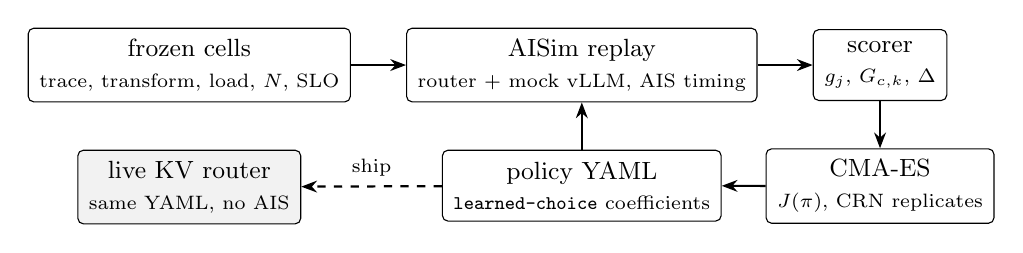
\begin{tikzpicture}[
      node distance=6mm and 7mm,
      box/.style={draw, rounded corners=2pt, align=center, font=\small, inner sep=4pt, minimum height=9mm},
      arr/.style={-{Stealth[length=2mm]}, thick}]
    \node[box] (cells) {frozen cells\\\scriptsize trace, transform, load, $\Nw$, SLO};
    \node[box, right=of cells] (replay) {\aisim{} replay\\\scriptsize router + mock vLLM, \ais{} timing};
    \node[box, right=of replay] (score) {scorer\\\scriptsize $\good_j$, $\Gw_{\cell,\krep}$, $\clr$};
    \node[box, below=of score] (cma) {CMA-ES\\\scriptsize $\Jobj(\pol)$, CRN replicates};
    \node[box, below=of replay] (yaml) {policy YAML\\\scriptsize \lc{} coefficients};
    \node[box, below=of cells, fill=black!5] (live) {live KV router\\\scriptsize same YAML, no \ais{}};
    \draw[arr] (cells) -- (replay);
    \draw[arr] (replay) -- (score);
    \draw[arr] (score) -- (cma);
    \draw[arr] (cma) -- (yaml);
    \draw[arr] (yaml) -- (replay);
    \draw[arr, dashed] (yaml) -- node[above, font=\scriptsize] {ship} (live);
  \end{tikzpicture}
  \caption{The training loop. A policy is a YAML file read by the router's builtin policy catalog,
    so each CMA-ES candidate costs a new YAML and a set of replays, with no rebuild. \ais{} times
    the simulated engines and so shapes the score; the headline policy never reads it.}
  \label{fig:loop}
\end{figure}

\paragraph{How ``better'' is decided.}
The comparison is on equal footing. Every policy, the learned arms and each of 11 tuned heuristic
baselines, is one configuration tuned on the pooled train cells with the same CMA-ES budget and
restarts and selected on validation; the best baseline, and by the same rule the headline learned
arm, are chosen on fresh validation replicates (\cref{sec:baselines,sec:eval}).
% src: CR/CONTRACT.md A2.1, A17.2; CR/facts/finalists.json selection
The comparison is made once, on a test set frozen with SHA-256 hashes before any tuning. Its 60
cells come from 12 independent workload segments and hold out time windows, agent plays, session
seeds, a trace family, transform ranges and worker counts. The headline is a one-sided exact
Wilcoxon signed-rank test over the segments, registered before training. Reported but not tested
are robustness to the SLO scale and definition, to stale router state (replay gives the router
perfectly fresh cache and load information, a live router does not) and to engine timing, and a
check of the ranking on GPUs.
% src: CR/facts/HEADLINE_TEST.json; CR/facts/test_freeze.json; CR/CONTRACT.md A5, A13, A14

\paragraph{What we found.}
% src: CR/facts/test_results.json headline, report_must_state; CR/facts/fairness_in_class_heuristic.json;
%      CR/facts/robustness.json; CR/audits/phase2-mid/gaming-concentration.md
Stated as the final audit allows: in AIS-timed simulation, the learned router M1-v2 beats the
branch's ported heuristics, each tuned with an equal budget. Against the validation-selected best
baseline, tuned \policy{ramjet}, it is ahead on 10 of the 12 test segments and on all 8 informative
ones (the 4 session segments tie at ceiling), with a segment-mean clipped log-ratio of $+0.0316$
and one-sided exact Wilcoxon $p = 0.0017$ (\cref{sec:res-headline}). It keeps first place among the
robustness finalists under router-state lag of 10 to \SI{200}{ms} and under four engine-timing
perturbations, and it ranks first under all four alternative definitions of a good request. Four
qualifications travel with the result.
\begin{itemize}
  \item Only the sign is a claim: the effect is below the pre-registered minimum detectable effect
    (0.038) and below the spread the timing perturbations induce (0.060).
  \item It is not ``learning beats every heuristic''. The baseline pool holds the branch's ports as
    implemented, and its \policy{lmetric} port lacks LMetric's queued-prefill term (a fix made to the
    port after the campaign froze adds it; \cref{sec:ports}). Faithful LMetric
    lies inside the learned model's class; untuned, it beats every tuned baseline on validation, and
    with the default cost it reproduces 53--66\% of the learned model's validation margin
    (\cref{sec:res-fairness}).
  \item It is a request-count property. A token-weighted goodput is mixed, and prompts of 32K
    to 64K tokens see higher time to first token than under \policy{ramjet}
    (\cref{sec:gaming}).
    % src: CR/facts/test_results.json report_must_state MS-F1-ttft (32K-64K p90 +0.135, 11/12; >= 64K
    %      filtered +0.021, 3/7, p 1.0, so the TTFT statement stops at 64K)
  \item Black-box search games a request-count objective. The first tuned model kept a worker
    whose requests were all bad; constraining load coefficients so that load cannot attract
    removed it, and every later learned arm runs under that constraint (\cref{sec:gaming}).
\end{itemize}
A pre-registered live check then served six of the $\Nw = 4$ test cells on H100 GPUs with Dynamo's
router running the same policy files (\cref{sec:live}). The live ranking of the six policies checked
agrees with simulation (pooled Kendall $\kendall$-b 1.00), and M1-v2 leads \policy{ramjet} in each of the
five cells where simulation predicts a lead, each time by more than the registered noise bar. The
check validates the ranking and that sign only: with one run per policy on six cells chosen after the
test pass, it says nothing about the headline's magnitude, and live goodput departs from simulation
by policy-dependent factors of 0.72 to 2.18, enough that on one cell the simulated gain over the
default router is not reproduced beyond live noise.
% src: CR/facts/live_results.json wording, primary.kendall_tau.k0 (tau_b 1.0), primary.sign_agreement
%      (5 of 5, beyond_noise_agree 5); CR/report/LIVE.md 15.2 (0.72-2.18; sessions not reproduced beyond
%      live noise), 15.7

\paragraph{Contributions.}
\begin{itemize}
  \item A description of Dynamo's worker-selection API as routing primitives, with the default
    cost function and nine other catalog policy types written in that vocabulary, and a list of the
    major caveats the campaign uncovered in the API, the replay host and the workloads, each with
    its evidence and status (\cref{sec:background}).
  \item \lc{}, a deployable worker-selection policy for Dynamo's router plugin catalog: a
    discrete-choice model over router-observable features that contains the default router as one
    coefficient setting and reads no simulator signal (\cref{sec:model}).
  \item A tuning method for routing policies in replay: CMA-ES on an episodic, windowed goodput
    objective with common-random-number workload replicates, applied with the same budget,
    restarts and selection rule to the learned model and to every heuristic baseline
    (\cref{sec:training,sec:baselines}).
  \item An objective and evaluation protocol for routing studies: goodput defined by inter-token
    latency and end-to-end slowdown over a request's own uncontended latency, measured in a window
    that excludes warm-up and drain; held-out worker counts; a pre-registered test over independent
    workload segments; and staged adversarial audits (\cref{sec:setup,sec:eval}).
  \item Results with their scope: the headline and its strata, worker-count extrapolation, the
    model ladder, the learned coefficients, robustness, the objective-gaming finding and its
    remedy, the secondary metrics that bound the claim, and a pre-registered live GPU check of the
    ranking (\cref{sec:results,sec:gaming,sec:live}).
\end{itemize}

\paragraph{Reading guide.}
\Cref{sec:background} introduces the routing primitives, the policies and the caveats.
\Cref{sec:setup} defines the decision and the objective, \cref{sec:simulator} the simulator and
workloads, \cref{sec:model} the policy and \cref{sec:training} its training. \Cref{sec:baselines}
describes how the baselines are tuned, \cref{sec:eval} the evaluation protocol, \cref{sec:results}
the results and \cref{sec:gaming} the concentration findings. \Cref{sec:live} reports the live GPU
validation. \Cref{sec:threats} discusses limitations and threats to validity, and
\cref{sec:related} relates the work to prior research. Labels of the form A$n$ refer to the
campaign contract's numbered amendments and LR-$n$ to the numbered lessons of its literature
review; both are part of the campaign record (\cref{app:repro}). Every number traces to a campaign
record named in a comment in the \LaTeX{} source.

% SPDX-FileCopyrightText: Copyright (c) 2026 NVIDIA CORPORATION & AFFILIATES. All rights reserved.
% SPDX-License-Identifier: Apache-2.0
%
% ROLE (operator request R1, CR/facts/PAPER_REQUESTS.md): routing primitives and the Dynamo
%   worker-selection API; the default cost function in that vocabulary; how each pedagogical cost
%   function (the ported policies) fits under it; the learned policy as a generalization; and the
%   major caveats the campaign uncovered, each with evidence and status. Split for a clean main text
%   (restructure plan, base <commit-50>): the main text keeps the API's composition, the default cost,
%   tab:api-policies, the learned generalization and a highlight of the caveats that shape results;
%   eligibility, declared inputs, request facts, catalog loading, the default picker's details and
%   the per-port rules are in appendix-api.tex (app:api, app:ports), and the full caveat table is
%   in appendix-caveats.tex (app:caveats, tab:caveats).
% EVIDENCE: WT/lib/kv-router/src/plugins/worker_selection.rs and worker_selection/{context,inputs,
%   config}.rs; WT/lib/kv-router/src/scheduling/{filter.rs,selector/policy.rs,config.rs};
%   WT/lib/router-plugins/builtin/src/{default/,default.rs,two_tier_cost_fn.rs,lmetric.rs,ramjet.rs,
%   dualmap.rs,chwbl.rs,llm_d/,sticky_session.rs,thunderagent/,learned_choice/}; caveats:
%   CR/facts/{UPSTREAM_FOLLOWUPS.md,DEVIATIONS.md,setup.json,agentx_lowered.json,lag_patch.json,
%   robustness.json,live_smoke.json}, CR/audits/{setup,build,phase2-mid,final}/.
% STATUS: final for this draft.

\section{Background: routing primitives and Dynamo's worker-selection API}
\label{sec:background}

Every routing rule in this study, Dynamo's default, the ported heuristics and the learned policy,
runs through one interface: Dynamo's worker-selection API, a contract between the router
\emph{host}, which owns the request path and the shared state, and a \emph{policy}, which turns that
state into a choice. This section describes the interface as a small set of routing primitives,
writes the default cost function and every other catalog policy in its vocabulary, shows how the
learned policy generalizes them, and highlights the caveats that bound the results. The vocabulary
is the one the code uses.\footnote{Type and method names are those of the router's plugin API on
  the study's branch.}
% src: WT/lib/kv-router/src/plugins/worker_selection.rs (module doc: "Public filter, scorer, and
%      picker contracts and their input signals")

% ---------------------------------------------------------------------------------------------
\subsection{The decision and what the host owns}
\label{sec:api-host}

For each request $j$ the host builds a \emph{candidate table} of eligible workers; eligibility and
pins are the host's and always win over a policy's preference (\cref{app:api}).
% src: WT/lib/kv-router/src/scheduling/filter.rs (RoutingEligibility); scheduling/selector/policy.rs
%      ("Explicit request pins remain mandatory regardless of this option")
The host also owns the state a policy reads. It keeps the KV index that the engines' cache events
feed and computes each candidate's prefix overlap with the request, per cache tier; it books the
load of every request it dispatches (prefill tokens in flight, decode blocks, active requests); and
it knows each worker's configured KV capacity. A policy owns only its decision and whatever private
state it chooses to keep, such as a random generator, a session map or a sliding window. This split
is what makes a policy portable: the same policy file runs wherever a host can fill the inputs it
declares, including the offline replay used here (\cref{sec:aisim}).

% ---------------------------------------------------------------------------------------------
\subsection{Filters, scorers and pickers}
\label{sec:api-components}

A worker-selection policy is an ordered composition of three kinds of component
(\cref{fig:api}).
\begin{description}
  \item[\code{WorkerFilter}] keeps or drops one eligible candidate. Filters run in declaration
    order and can only shrink the set.
  \item[\code{WorkerScorer}] writes one finite, lower-is-better cost for every surviving candidate
    in a single call. The host validates each contribution and adds the contributions of all
    scorers, so scorers compose additively.
  \item[\code{WorkerPicker}] receives the surviving candidates with their total costs and returns
    one row. It may ignore the costs entirely.
\end{description}
% src: worker_selection.rs (WorkerFilter::keep, WorkerScorer::score "Write one finite,
%      lower-is-better contribution", WorkerPicker::pick); selector/policy.rs (ComposedPolicyState:
%      filters, scorers, picker; WorkerSelectionPolicy::new_with_filters)
None of the builtin policies in this study uses a filter; candidate restriction, where a policy
needs it, happens inside its picker. Every builtin policy is therefore ``scorers plus a picker'',
and the interesting differences are in which inputs each reads and whether its choice for one
worker depends on the other candidates.
% src: grep of WT/lib/router-plugins/builtin/src for "impl WorkerFilter for": no builtin filter

A component declares the optional worker signals it reads, such as cache overlap (\code{CACHE}),
router-tracked load (\code{LOAD}), a modeled prefill backlog (\code{PREFILL\_TIME}) and a cost
multiplier from the request's preferred routing constraints (\code{PREFERRED\_TAINT}), and the host
materializes only those; a policy also reads request facts such as the prompt length, its prefix
hashes and the session context (\cref{app:api}).
% src: worker_selection/inputs.rs (WorkerInputs); worker_selection/context.rs (WorkerSelectionContext)

\paragraph{The policy catalog.}
A deployment selects policies with a YAML file. Its \code{worker\_selection} block names one
instance per worker role (aggregated, prefill, decode, encode) and lists named instances, each a
catalog \code{type} with a \code{parameters} mapping (\cref{fig:api}); \cref{app:api} describes how
the host loads and validates the catalog.\footnote{The offline replay host on this study's branch
  runs the same catalog; on Dynamo's main branch at the time of the study, replay rejected catalog
  policies selected by YAML.}
% src (footnote): CR/facts/UPSTREAM_FOLLOWUPS.md "Straight-main lane outcomes" #1 ("on main replay
%      rejects YAML-selected catalog policies")
% src: worker_selection/config.rs (RawWorkerSelectionConfig: aggregated, prefill, decode, encode,
%      instances)

\begin{figure}[tbp]
  \centering
  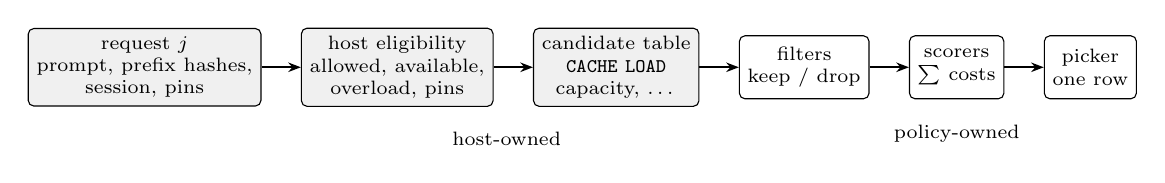
\begin{tikzpicture}[
      node distance=4mm and 5mm,
      box/.style={draw, rounded corners=2pt, align=center, font=\scriptsize, inner sep=3pt,
        minimum height=8mm},
      host/.style={box, fill=black!6},
      arr/.style={-{Stealth[length=1.6mm]}, thick}]
    \node[host] (req) {request $j$\\prompt, prefix hashes,\\session, pins};
    \node[host, right=of req] (elig) {host eligibility\\allowed, available,\\overload, pins};
    \node[host, right=of elig] (table) {candidate table\\\code{CACHE} \code{LOAD}\\capacity, \dots};
    \node[box, right=of table] (filters) {filters\\keep / drop};
    \node[box, right=of filters] (scorers) {scorers\\$\sum$ costs};
    \node[box, right=of scorers] (picker) {picker\\one row};
    \draw[arr] (req) -- (elig);
    \draw[arr] (elig) -- (table);
    \draw[arr] (table) -- (filters);
    \draw[arr] (filters) -- (scorers);
    \draw[arr] (scorers) -- (picker);
    \node[font=\scriptsize, below=2mm of $(elig.south)!0.5!(table.south)$] {host-owned};
    \node[font=\scriptsize, below=2mm of scorers.south] {policy-owned};
  \end{tikzpicture}

  \vspace{4pt}
  \begin{minipage}{0.7\linewidth}
\begin{footnotesize}
\begin{verbatim}
worker_selection:
  aggregated: candidate      # instance for full requests
  instances:
    - name: candidate
      type: ramjet           # any catalog type
      parameters:
        alpha: 0.883
        max_affinity_blocks: 68
        load_unit_tokens: 4552
\end{verbatim}
\end{footnotesize}
  \end{minipage}
  \caption{Top: one worker selection. The host fixes the eligible candidates and fills the inputs the
    policy's components declared; the policy's filters, scorers and picker turn them into one row.
    Bottom: the policy file that selects a catalog type and its parameters; the parameters shown are
    the tuned \policy{ramjet} configuration that serves as the best baseline in this study.}
  \label{fig:api}
\end{figure}
% src (ramjet parameters): CR/facts/finalists.json headline.val_best_baseline.spec.parameters
%      (alpha 0.8828774076622825, max_affinity_blocks 68, load_unit_tokens 4552,
%      affinity_block_tokens 512, basis relative)

% ---------------------------------------------------------------------------------------------
\subsection{Dynamo's default cost function}
\label{sec:default-cost}

% src: WT/lib/router-plugins/builtin/src/default/scorer.rs (score_worker, aggregated branch);
%      knobs in default/parameters.rs. The formula below is the aggregated, prefill-tracking path
%      replay uses; decode-only, host/disk-tier, shared-cache and taint terms are omitted.
In the API's terms, the default router (\defaultcf{} in the catalog) is one scorer and one picker.
The scorer declares \code{LOAD}, \code{PREFERRED\_TAINT} and, unless its overlap credit is zero,
\code{CACHE}, and assigns each candidate a cost in KV blocks:
\begin{equation}
  \label{eq:default-cost}
  \cdef_i = \bpf \max\!\Big(0,\ \frac{\Lpf_i + \ISL_j}{16} - \bov\,\gamma_i\,\ovl_i\Big)
           + \Ldec_i + \breq \Lreq_i,
\end{equation}
where $\ovl_i$ is the candidate's device-tier overlap in blocks, $\Lpf_i$ its active prefill tokens,
$\Ldec_i$ its decode cost blocks (including this request's new blocks), $\Lreq_i$ its active
requests, 16 the KV block size, and
\(
  \gamma_i = \big(1 + \bdecay\,(\Lpf_i - \min_{i' \in \cand}\Lpf_{i'})/(16\,\reqblocks_j)\big)^{-1}
\)
discounts the overlap credit of workers with more queued prefill than the least-loaded one. The
shipped defaults are an overlap credit $\bov = 1$, a decay $\bdecay = 0$, a prefill load scale
$\bpf = 1$ and a decode request weight $\breq = 0$, so the default router minimizes the prefill
blocks the worker would still have to compute plus its decode load.\footnote{The full scorer also
  credits host- and disk-tier and shared-cache hits, has a separate branch for decode-only workers,
  and multiplies the cost by a preferred-taint factor; none of these enter the aggregated,
  device-tier-only setting studied here, in which replay requests carry no taint preferences.}
% src (taint): WT/lib/mocker/src/replay/offline/extensions/kv_router/mod.rs (routing_constraints:
%      RoutingConstraints::default(), so preferred_taints is empty and the multiplier is absent)

The picker takes the minimum cost; with a \code{router\_temperature} above zero it samples from a
softmax over costs normalized to their range across the candidates, so at positive temperature the
default is set-dependent. \Cref{app:api} gives its tie-breaking, seeding and session-affinity
details.
% src: default/picker.rs (softmax_sample_index: range-normalized costs)

% ---------------------------------------------------------------------------------------------
\subsection{The ported cost functions as instances of the API}
\label{sec:baseline-policies}

\Cref{tab:api-policies} writes every catalog policy type of the study in the API's vocabulary: its
components, the inputs and request facts it reads, whether its choice for one worker depends on the
other candidates (set dependence), the state it keeps, and the parameters this study tunes. The
pedagogical value of the table is that the policies differ along a few axes only. Most are a single
picker over \code{CACHE} and \code{LOAD}; they differ in how they combine overlap with load
(additive, multiplicative, thresholded or lexicographic), in whether they restrict candidates by a
hash of the prompt prefix, and in whether they compare a worker with the rest of the set. The
router's round-robin mode is not a catalog policy: it sends requests to the workers in turn, reads
neither cache nor load, has no parameters, and serves as a floor.
% src: CR/CONTRACT.md "Policy YAML" (round-robin uses router_mode="round_robin", no YAML)
\Cref{app:ports} states each rule in full and lists where the ports differ from the published
methods; \cref{sec:ports} discusses the difference that bears on the headline.

% src: per-row components and inputs from the WorkerSelectionPolicy::new calls and the
%      required_worker_inputs of WT/lib/router-plugins/builtin/src/{default.rs, default/scorer.rs,
%      two_tier_cost_fn.rs, lmetric.rs, ramjet.rs, dualmap.rs, chwbl.rs, llm_d/precise_prefix.rs,
%      llm_d/optimized_baseline.rs, sticky_session.rs, thunderagent/worker_selection/mod.rs,
%      learned_choice/mod.rs}; request-fact accessors grepped per file (prefix_hashes: chwbl,
%      dualmap, lmetric, learned_choice v2; session_context: sticky_session, learned_choice;
%      policy_class and worker_capacity: precise_prefix; worker_capacity: learned_choice;
%      affinity_target: thunderagent); exclusive affinity: default, sticky_session, learned_choice;
%      tuned parameters: CR/facts/phase2_prep.json spaces (tab:baseline-spaces)
{\footnotesize
\setlength{\LTcapwidth}{\linewidth}
\setlength{\tabcolsep}{4pt}
\begin{longtable}{@{}P{0.17\linewidth}P{0.18\linewidth}P{0.14\linewidth}P{0.18\linewidth}P{0.12\linewidth}P{0.1\linewidth}@{}}
\caption{Catalog policy types as compositions of API components. S: scorer; P: picker (every
  policy has exactly one). Inputs: declared \code{WorkerInputs} (C = \code{CACHE}, L = \code{LOAD},
  PT = \code{PREFILL\_TIME}, T = \code{PREFERRED\_TAINT}). Request facts beyond the prompt length:
  hashes = prefix hashes, session = session context, capacity = advertised KV capacity.
  Set-dependent: whether a candidate's score or eligibility depends on the other candidates at the
  shipped parameters.}
\label{tab:api-policies}\\
\toprule
Type (variants) & Components & Inputs, request facts & Set dependence & State & Tuned here \\
\midrule
\endfirsthead
\toprule
Type (variants) & Components & Inputs, request facts & Set dependence & State & Tuned here \\
\midrule
\endhead
\bottomrule
\endfoot
\code{dynamo-default-}\allowbreak\code{cost-fn} & S default cost; P min cost (softmax if $\temp > 0$) & C, L, T &
  through $\gamma_i$ if $\bdecay > 0$, and the softmax & random generator & 5 knobs (M0,
  \cref{sec:ladder}) \\
\code{dynamo-two-tier-}\allowbreak\code{cost-fn} & P lexicographic (load tier, cache tier) & C, L &
  yes: request spread and best overlap across the set & none & 3 thresholds \\
\policy{lmetric} & P min of a product & C, L, hashes &
  hot-spot classes (holders against non-holders) & class window & 2 \\
\policy{ramjet} & P max of affinity minus load & C, L &
  yes: affinity relative to the warmest candidate & tie rotation & 3 \\
\policy{dualmap} & P two hashed candidates, warmer unless over budget & C, L, hashes &
  yes: candidates fixed by hash & prefix window & 3 \\
\policy{chwbl} & P hashed owner within a load bound & L, hashes &
  yes: bound relative to the set mean & none & 2 \\
\code{llm-d-precise-}\allowbreak\code{prefix} & S prefix, S queue, S KV utilization; P max score & C, L,
  capacity, policy class & yes: queue score scaled by the set's range & tie rotation & 4 \\
\code{llm-d-optimized-}\allowbreak\code{baseline} (throughput, modeled) & S token load; P sticky filter and TTFT gate &
  C, L (PT if modeled) & yes: sticky set and TTFT gate & tie rotation & 3 \\
\policy{sticky-session} (hard, bounded) & S default cost; P session's worker or min cost &
  C, L, T, session & bounded: request count against the set mean & session map, generator &
  5 or 6 \\
\policy{thunderagent} & S prefill and decode load; P classifier's target or min cost & L, affinity
  target & no & in its request classifier & not evaluated \\
\midrule
\lc{} (this work) & S default cost (feature 0); P utility argmax & C, L, T, capacity, session,
  hashes (\code{v2}) & \code{v1} at rank 0: no; \code{v2} and context terms: yes & session map,
  generator & 7 to 22 coefficients (headline league) \\
\end{longtable}
}

% ---------------------------------------------------------------------------------------------
\subsection{The learned policy as a generalization}
\label{sec:api-learned}

Each of these rules hand-picks a functional form over a few of the declared inputs. \lc{}
(\cref{sec:model}) instead scores every candidate with one utility that is linear in a fixed vector
of features computed from the same inputs, and lets the coefficients be tuned. It is built from the
same parts as the rules it generalizes: the default cost function's own scorer supplies its first
feature, and a picker computes the rest and takes the argmax. Several of the heuristics are points,
or limits, of its parameter space.
\begin{itemize}
  \item $\theta = -\basis{0}$ is the default router (\cref{sec:parity}).
  \item A large positive session coefficient is hard stickiness (\cref{sec:sticky}).
  \item With the extended feature set \code{v2}, $\theta = -(\basis{8} + \basis{10})$ takes the
    argmin of LMetric's product with the queued-prefill term, and $-(\basis{9} + \basis{10})$
    reproduces the branch's \code{lmetric} port as evaluated, without its hot-spot filter
    (\cref{sec:features}).
  \item \code{v2}'s \code{hash\_home} indicator marks the two rendezvous-hashed candidates of a
    prompt prefix, the candidate set of DualMap and Lodestar \citep{yuan2026dualmap,lim2026lodestar}.
  \item Set-relative features and context terms let the comparison between two workers depend on
    the others (\cref{sec:context}), as the queue score of \policy{llm-d-precise-prefix} or the
    relative basis of \policy{ramjet} do by construction.
\end{itemize}
What it cannot express are hard thresholds and lexicographic rules (two-tier's tiers, DualMap's
budget, CHWBL's bound, the optimized baseline's TTFT gate) and history-dependent windows, which a
smooth utility can only approximate. The study's question is whether tuning a generalization
of this kind, with the same budget as each hand-picked rule, finds a better trade on one deployment.

% ---------------------------------------------------------------------------------------------
\subsection{Caveats that bound the results}
\label{sec:caveats}

% src: rows 1, 2, 3, 9, 10, 13 and 15 of tab:caveats (sections/appendix-caveats.tex), whose row
%      comments name the evidence
Building, calibrating and auditing the study surfaced properties of the API, the replay host and the
workloads that can change which policy wins, and several of them shape the results. Replay's router
state is perfectly fresh, while a live router sees cache events and load late (caveat 1;
\cref{sec:res-robustness,sec:live}). Replay fills \code{expected\_output\_tokens} with the true output
length, a value no live router has; no learned feature reads it (caveat 2). Host knobs change what
the inputs mean: without assumed KV reuse every prefix hash is unique to its request, so prefix-keyed
policies lose their keys, and the learned policy must run with its training-time knobs (caveat 3;
\cref{sec:threats-scope}). Logged arrival timestamps are quantized, so the harness spreads arrivals
per replicate (caveat 9; \cref{sec:replicates}). No AgentX play (one recorded agent run;
\cref{sec:workloads}) fits a 32K context, so the deployment runs at 128K with YaRN context extension
(a factor of 4 over the model's original \num{32768} tokens), where \ais{}'s accuracy is least
validated, and \aisim{} prices a mixed prefill
pass at the batch mean, an artifact a search could exploit (caveats 10 and 13;
\cref{sec:threats-sim,sec:gaming}). Finally, the request-count objective can be gamed (caveat 15;
\cref{sec:gaming}). \Cref{app:caveats} lists all 15 with their evidence and status (fixed, follow-up,
inherent).
% src (YaRN gloss): CR/facts/live.json ("--max-model-len 131072 with YaRN (factor 4, original 32768)");
%      CR/config/engine.json max_model_len note ("131072 per operator (YaRN)"); restructure round 1, E4
% src (mixed prefill pricing): CR/facts/UPSTREAM_FOLLOWUPS.md #17
%      (AISim, the replay engine, prices a mixed prefill pass; it calls AIS predict_prefill on batch means)

% SPDX-FileCopyrightText: Copyright (c) 2026 NVIDIA CORPORATION & AFFILIATES. All rights reserved.
% SPDX-License-Identifier: Apache-2.0
%
% ROLE: define the decision (which worker serves a request), what the router can observe, how load
%   is applied, and the objective every policy is scored by. Everything later refers back here.
% CLAIMS: definitional, plus the reasons for each definition (slowdown rather than raw latency,
%   windowed rather than makespan goodput, clipped log-ratio rather than mean ratio).
% EVIDENCE: CR/CONTRACT.md (Deployment, A2, A5.2, A14, A17.2); CR/config/engine.json;
%   WT/benchmarks/learned_routing/learned_routing/{goodput.py,e0.py,train.py};
%   CR/facts/{calibration.json,setup.json,build_workloads.json}; CR/literature/LESSONS.md LR-01,
%   LR-08, LR-09; WT/lib/router-plugins/builtin/src/learned_choice/FEATURES.md.
% STATUS: definitions settled (frozen at calibration, lr-cells-v5).

\section{Problem and objective}
\label{sec:setup}

This section fixes what a routing policy decides, what it may observe, how load is applied, and the
score by which every policy, learned or heuristic, is compared.

\subsection{The routing decision}
\label{sec:decision}

\paragraph{Deployment.}
% src: CR/CONTRACT.md "Deployment (operator-fixed)"; CR/config/engine.json mock_engine_args;
%      CR/facts/setup.json kv_capacity
A deployment runs $\Nw$ identical aggregated workers, each a vLLM engine serving Qwen3-32B with
tensor parallelism 2 on H100 SXM GPUs, so prefill and decode share a worker. Each worker holds
\num{18863} KV blocks of 16 tokens, \num{301808} tokens in all. The study covers
$\Nw \in \{2, 4, 6, 8, 16, 32\}$; heterogeneous worker sets are out of scope (Amendment A5.2).
The router never holds a request back: \code{router\_queue\_threshold} is left unset, which
disables router-side queueing; an ablation that tuned it jointly found no measurable gain
(\cref{sec:res-ladder}).
% src: WT/lib/kv-router/src/scheduling/config.rs test queueing_enabled_reflects_synthetic_threshold
%      ("With default config, queueing is disabled"); binding default router_queue_threshold=None
%      (WT/lib/bindings/python/rust/llm/entrypoint.rs:134)

\paragraph{A sequential discrete choice.}
When request $j$ arrives at time $a_j$, the router's worker-selection policy $\pol$ picks one
worker from the eligible candidate set $\cand \subseteq \{1,\dots,\Nw\}$. Three properties shape
the problem.
\begin{itemize}
  \item \emph{The choice is sequential.} The chosen worker computes the uncached part of $j$'s
    prompt and keeps the resulting KV blocks, which later requests that share the prefix can reuse
    and which may evict other prefixes' blocks. Request $j$ also adds to that worker's prefill and
    decode load until it completes. A decision's cost or benefit therefore lands on other requests,
    often much later in simulated time, and no per-decision label exists. Policies are scored on
    whole episodes (\cref{sec:objective}).
  \item \emph{The worker set varies.} $\Nw$ differs across deployments, and $\cand$ can be smaller
    than $\Nw$ when the host marks workers ineligible. A policy defined on a fixed-length vector of
    all workers' states would need retraining for every $\Nw$. A policy that scores each candidate
    with one shared function and picks the best applies to any $|\cand|$. This is the
    discrete-choice form of the learned policy (\cref{sec:model}), and it is what lets the test
    set hold out worker counts that training never saw.
  \item \emph{The choice is made online.} It runs once per request on the router's request path,
    from information available at $a_j$, so it must be cheap and must not depend on the future.
\end{itemize}

\paragraph{What the router observes.}
% src: WT/lib/router-plugins/builtin/src/learned_choice/FEATURES.md "Feature set v1",
%      "Excluded inputs", "Information parity with the live router"
At decision time a policy sees, through the router plugin API (\cref{sec:api-components}):
\begin{itemize}
  \item the request: its prompt length $\ISL_j$, its prefix block hashes and an optional session
    identifier;
  \item per candidate, the router's cache estimate: blocks of overlap with the request's prefix and
    the estimated number of cached tokens;
  \item per candidate, load the router tracks from its own dispatches: active prefill tokens,
    decode blocks and active requests;
  \item per candidate, its configured KV capacity in blocks.
\end{itemize}
The learned policy reads nothing else. In particular it ignores the request's expected output
length, which offline replay fills with the true output length, and every performance-model
estimate; engine-internal state such as waiting-queue length or KV usage is not available to it.
Because it uses only these inputs, the artifact trained in replay is the one the live router runs
(\cref{sec:integration}). Replay applies cache events to the
router's index at once, while a live router sees them late; this difference is a robustness check
(\cref{sec:robustness}), not part of the problem definition.

\subsection{Load modes}
\label{sec:loadmodes}

% src: CR/cells/{train,val,test}.jsonl load.mode by family (train: Mooncake 12 open + 6 closed,
%      sessions 6 open + 2 closed, AgentX 8 lanes; test: 31 open, 15 closed, 14 lanes);
%      CR/facts/calibration.json rules.levels (units), lessons.LR-09 (causal session release kept);
%      WT/benchmarks/learned_routing/learned_routing/goodput.py (occupancy units); CR/CONTRACT.md A3
A cell offers its trace to the workers in one of three ways, which differ in what a policy can
change.
\begin{description}
  \item[Open loop.] Requests arrive at the trace's timestamps, compressed or stretched by a speedup
    factor that sets the load. A policy cannot change when requests arrive, only how well they are
    served. In multi-turn session cells the session start times are fixed this way, while each
    follow-up turn is released a think time after the previous turn completes, as in a real
    conversation.
  \item[Closed loop.] A fixed number of sessions is in flight; a session holds its slot through its
    think times, and a new session starts when one ends. Each Mooncake trace row is its own
    one-turn session. A policy that serves requests faster also receives more of them, so
    throughput depends on the policy.
  \item[Agentic lanes.] A fixed number of lanes each run one recorded agent play at a time. Inside
    a play, requests follow the recorded dependency graph (sequential turns, subagent spawns and
    joins, tool delays), and a lane starts its next play when the previous one ends.
\end{description}
Mooncake, FAST25 and session cells run in open and closed loop, and AgentX cells in lanes;
calibration sets each cell's load (\cref{sec:calibration}). Results are reported per mode, because
open and closed systems respond to scheduling differently \citep{schroeder2006open}. Session and
agentic work is released causally because replaying follow-up turns at their recorded timestamps
would fix a release schedule, and cache state, that a different policy is supposed to change
\citep{rajib2026agentservesim,alomar2023causalsim}.
% src: CR/literature/LESSONS.md LR-09 (AgentServeSim pdf p.1-2, p.4; CausalSim pdf p.1-3;
%      Schroeder pdf p.10-11), VERIFIED

\subsection{Objective}
\label{sec:objective}

\paragraph{Good requests.}
% src: CR/CONTRACT.md A2.2 (operator decision: no TTFT SLO); WT/benchmarks/learned_routing/
%      learned_routing/goodput.py (a2_good, token_form_good, completed, E2E_REL_TOL = 1e-6)
The deployment's service objective, set by the operator, concerns the pace of the token stream and
the total request latency, not the time to first token. A request is \emph{good} iff it completes
and
\begin{equation}
  \label{eq:good}
  \good_j = \mathbf{1}\!\left[\ITLbar_j \le \Imax\right]\cdot
            \mathbf{1}\!\left[\EtoE_j \le \Smax\,\Ezero(\ISL_j,\OSL_j)\right],
\end{equation}
where $\ITLbar_j = (\EtoE_j - \TTFT_j)/(\OSL_j - 1)$ is the mean inter-token latency, the ITL
clause is skipped when $\OSL_j \le 1$, and the slowdown clause allows a relative tolerance of
$10^{-6}$ for floating-point rounding. Rejected, errored and incomplete requests are never good.
$(\Imax, \Smax)$ is one pair per workload family (\cref{tab:notation}). $\TTFT_j$ is reported but
is not part of \cref{eq:good}; it enters only through $\EtoE_j$.

\paragraph{The reference latency.}
% src: WT/benchmarks/learned_routing/learned_routing/e0.py (method ais-chunked-estimator-v2;
%      "matches 17,233 isolated single-request replays to within 2e-8 relative");
%      CR/facts/STATE.md audit(calibration/independent-rerun r1) (own E0 == harness within
%      1.11e-8 on 880,139 pairs); CR/CONTRACT.md A2.2
$\Ezero(\ISL,\OSL)$ is the request's latency alone on an idle worker with no prefix reuse: a full
chunked prefill of $\ISL$ tokens followed by $\OSL - 1$ decode steps at batch size 1, timed by
\ais{}. It depends only on $(\ISL, \OSL)$ and is cached per pair. It agrees with isolated
single-request replays to within $2\times10^{-8}$ relative, and an independent audit's own
computation matched it on \num{880139} pairs. $\Ezero$ is used only for scoring; no policy sees it.

\paragraph{Why a slowdown bound.}
% src: CR/facts/setup.json long_context.evidence.single_request_ttft_ms_ais (1024: 55.49 ms,
%      8192: 475.97 ms, 32768: 2,550.45 ms, 120000: 17,815.54 ms);
%      CR/facts/build_workloads.json traces.flat.<family>.isl_mean (mooncake 8,590.0;
%      fast25_conversation 12,035.1; fast25_synthetic 15,325.5); agentx.selection.predicate
%      (in + max(out, 1) <= 131072); CR/literature/LESSONS.md LR-08 (SMetric pdf p.8, VERIFIED;
%      CR/literature/txt/llm-routing/wang2026-smetric.txt line 1135)
Request sizes vary widely. Mean prompt lengths are \num{8590} tokens on Mooncake
and \num{12035} to \num{15326} on the FAST25 traces, and AgentX plays were admitted as long as
every request, prompt plus output, fits the \num{131072}-token context. In \ais{}'s timing, prefill
alone on an idle worker takes \SI{55.49}{ms} at \num{1024} tokens, \SI{475.97}{ms} at \num{8192},
\SI{2550}{ms} at \num{32768} and \SI{17815.54}{ms} at \num{120000}. A single absolute bound on
end-to-end latency would be unattainable for the longest requests even on an idle worker, or slack
for the shortest. Fixed first-token deadlines have the same problem; SMetric's authors note that
providers typically set the TTFT deadline linear in the request length \citep{wang2026smetric}. Dividing by $\Ezero$ scales the bound
with each request's own unavoidable work: under the Mooncake bound $\Smax = 3.46625$, a request may
take up to about 3.5 times its uncontended latency, whatever its size.

Two properties of $\Ezero$ keep the bound fair across policies. It is policy independent, so every
policy is held to the same per-request bound. And it assumes no prefix reuse, so a cache hit lowers
$\EtoE_j$ but not $\Ezero$: a policy that earns more reuse finds the bound easier to meet, never
harder.

\paragraph{Why two clauses.}
The clauses catch different failures. For a long prompt, $\Smax\Ezero$ is dominated by prefill
time, so a slow token stream after a fast prefill can pass the slowdown clause; the ITL clause
catches it. Conversely, a request that waits a long time and then streams at an ordinary pace
passes the ITL clause and fails the slowdown clause. At the calibrated bounds the slowdown clause
does most of the work: at the calibration load nearest L2 on $\Nw = 8$, the ITL clause alone fails
0.6\% of $\piref$'s requests on sessions, 1.8\% on AgentX and 4.5\% on Mooncake, while 15\% of
requests are not good at L2 by construction.
% src: CR/facts/calibration.json sla.<family>.itl_only_fail_at_l2_grid.default
%      (synthetic_sessions 0.00625 at grid load 0.375; agentx 0.0178 at 3; mooncake 0.0449 at 9000)
%      and summary.sla.<family>.itl_only_fail_frac_default_at_L2; L2 = good fraction 0.85
%      (rules.levels). "Most of the work" is the inference 15% - 4.5% > 4.5%.
% check: the grid load is near but not at L2 (sessions 0.375 vs 0.380, AgentX 3 vs 3.388,
%        Mooncake 9000 vs 8797.97 per worker); keep "nearest L2".

\paragraph{Windowed goodput.}
% src: CR/CONTRACT.md A2.3; CR/facts/calibration.json rules.windows;
%      WT/benchmarks/learned_routing/learned_routing/goodput.py (measurement_window, _window_counts,
%      _completes_inside, _completion_end)
A cell's score is its windowed goodput $\Gw_{\cell,\krep}(\pol)$, good requests per simulated
second inside a measurement window $\win_{\cell}$ that starts after a warm-up. Its form depends on
the load mode. In open-loop cells the window is a fixed interval of arrival times, and
\begin{equation}
  \label{eq:goodput-open}
  \Gw_{\cell,\krep}(\pol) = \frac{1}{|\win_{\cell}|}\sum_{j:\ a_j \in \win_{\cell}} \good_j ,
\end{equation}
so a request that arrives in the window counts even if it finishes after it, and one that never
completes counts as not good. In closed-loop and lane cells, $\Gw$ counts the good requests that
\emph{complete} inside a half-open window, divided by its length. That window ends at full
occupancy, the last instant at which every session or lane slot is busy, so its end, and hence
its length, depends on the policy.

The window removes three distortions.
\begin{itemize}
  \item \emph{Drain.} The replay's native goodput divides good requests by the makespan, which
    includes the drain after the last arrival, so it mixes SLO attainment with how fast a policy
    clears the tail.
    % src: CR/literature/LESSONS.md LR-01 [code] aisimulate-core src/replay/report.rs 1807-1895
    %      (duration_ms = max(report_end, max terminal_time) - report_start), VERIFIED
    In closed loops and lanes, completions after full occupancy happen with fewer requests in
    flight, and in lane cells the lanes run out of plays at different times, so counting the tail
    would credit easy, under-loaded requests.
    % src: goodput.py module docstring "Completion-basis end rule (build audit r1 F1)"
  \item \emph{Cold start.} Caches start empty and session populations ramp up, so the first minutes
    of a replay are not the steady state the cell represents. The warm-up length matters: for
    open-loop session cells, a first calibration with a \SI{180}{s} warm-up gave $\piref$ a good
    fraction that moved by up to 0.353 when the warm-up history was doubled (9 of 12 cells beyond
    3 standard errors); with the adopted warm-up of two session lifetimes, doubling moves it by at
    most 0.014 (no cell beyond 3 standard errors).
    % src: CR/facts/calibration.json session_open_warmup.doubled_warmup_check.summary
    %      ("w180_vs_w2x|gf_default": max_abs_delta 0.3527, cells_abs_z_gt_3 9 of 12;
    %       "w1x_vs_w2x|gf_default": max_abs_delta 0.0142, cells_abs_z_gt_3 0 of 12)
  \item \emph{Deferral.} An objective that ignored requests finishing after the horizon would
    reward deferring work past it; Decima's learned scheduler did exactly this under a fixed
    horizon \citep{mao2019decima}. Counting in-window arrivals that finish late removes the
    incentive.
    % src: CR/literature/LESSONS.md LR-01 (Decima pdf p.7), VERIFIED
\end{itemize}
When every arrival is set by the trace, as in the open-loop Mooncake and FAST25 cells, the number
of in-window arrivals is the same for every policy on a replicate, so the ratio of two policies'
goodputs equals the ratio of their in-window good fractions. In closed-loop and lane cells
goodput also rewards throughput, which the policy legitimately controls there. SLO attainment as
the primary serving metric follows \citet{zhong2024distserve}.

\paragraph{SLO and load calibration.}
% src: CR/facts/calibration.json rules.sla, rules.levels, sla.<family>; CR/runs/calibrate-fix-r0/decisions.json
The bounds $(\Imax,\Smax)$ are fixed per family from runs of $\piref$ on train segments at
$\Nw = 8$, and each cell's load is one of three levels L1, L2, L3, at which $\piref$'s good fraction
is 0.95, 0.85 and 0.65. Levels are calibrated separately for every $\Nw$ and transform, on train
segments only, and both bounds and levels were frozen before any policy was tuned
(\cref{sec:calibration}). The bounds differ widely by family, from $\Smax = 1.16134$ on AgentX to
3.46625 on Mooncake, because each is anchored at its own family's load knee. Every cell therefore
sits where the default router is starting to miss its objective, the regime in which routing
changes outcomes; that the regime is defined relative to one baseline is a threat discussed in
\cref{sec:threats}.

\paragraph{Normalized score.}
% src: WT/benchmarks/learned_routing/learned_routing/train.py (pair_score, LOG_CLIP = ln 3,
%      TrainConfig.eps = 1e-3); CR/facts/HEADLINE_TEST.json per_cell_statistic;
%      CR/facts/gate.json full_plan.objective_cells_repeats ("pre-registered, LR-01")
Goodput levels differ by orders of magnitude across cells, so every comparison is a ratio on the
same cell and replicate:
\begin{equation}
  \label{eq:clr}
  \ratio_{\cell,\krep}(\pol,\pol') = \frac{\Gw_{\cell,\krep}(\pol)+\varepsilon}{\Gw_{\cell,\krep}(\pol')+\varepsilon},
  \qquad
  \clr_{\cell,\krep}(\pol,\pol') = \clip\!\left(\log \ratio_{\cell,\krep}(\pol,\pol'),\,-\clipb,\,\clipb\right),
\end{equation}
with $\varepsilon = 10^{-3}$ good requests per second. Both policies run on the same workload
replicate $\krep$ with the same tie-breaking seed (common random numbers, \cref{sec:noise}).
Training uses $\pol' = \piref$ (\cref{eq:objective}); the headline uses $\pol' = \pibase$
(\cref{eq:segstat}). The log makes the score symmetric, so doubling goodput on one cell and halving
it on another nets to zero. The clip limits any one cell to a factor of 3 either way, which matters
because a mean of raw ratios is dominated by the few cells where one policy collapses
\citep{agarwal2021precipice}, and such cells occur here. On all 9 open-loop session cells of the
train and validation splits, round-robin's goodput is 0.111 to 0.425 times the default router's,
and below 1/3 on 5 of them. A policy that far past its stability limit has no steady state, so the
ratio is not a stable quantity: on one cell, doubling the warm-up history halved it, from 0.118 to
0.055. The clip scores every ratio below 1/3 alike, so that unstable detail cannot drive training
or the headline.
% src: CR/audits/calibration/independent-rerun-r1.md F1 ("RR/default ratio is 0.111-0.425; 5 train/val
%      cells are below 1/3"; sessions-s1-base-n4-open-L3 0.118 -> 0.055 with doubled history;
%      "absorbs everything below 1/3"); Agarwal pdf p.2-3 (CR/literature/LESSONS.md LR-01, VERIFIED)
The clipped log-ratio was chosen over the mean of ratios at calibration, before any training.
% src: CR/facts/HEADLINE_TEST.json (written "calibration stage, before any training");
%      CR/facts/pilot.json decisions[1] (objective clipped_log_ratio, "pre-registered in HEADLINE_TEST.json")

\paragraph{What ``better'' means.}
% src: CR/CONTRACT.md A2.1, A17.2; CR/facts/HEADLINE_TEST.json; CR/CONTRACT.md A14
The headline compares the learned policy with the best baseline \emph{on the same footing}: each
policy, learned or heuristic, is one configuration tuned on the pooled train split with the same
CMA-ES budget and selected on validation (\cref{sec:training,sec:eval}). The best baseline $\pibase$
is the baseline with the highest mean clipped log-ratio on fresh validation replicates. The learned
side is chosen by the same rule among the learned variants that read only router-observable
signals, and the number of variants compared is reported. The comparison is made once, on the
frozen test set, by the pre-registered test of \cref{sec:headline}. Because the objective itself is
a modeling choice, the same test records are also re-scored with scaled bounds and with
alternative definitions of a good request: ITL alone, slowdown alone, and the ITL bound combined
with either a length-scaled TTFT bound or an absolute latency bound. These secondary analyses never
change the headline.

% SPDX-FileCopyrightText: Copyright (c) 2026 NVIDIA CORPORATION & AFFILIATES. All rights reserved.
% SPDX-License-Identifier: Apache-2.0
%
% The single notation table. Every section uses these symbols through the macros in
% macros.tex. A new symbol needs a row here first.
% Code names refer to WT/lib/router-plugins/builtin/src/learned_choice/ (Rust) and
% WT/benchmarks/learned_routing/learned_routing/ (harness); contract names to CR/CONTRACT.md.

\subsection{Notation}
\label{sec:notation}

\Cref{tab:notation} fixes the symbols used throughout. The campaign's contract, the policy's
specification (\code{FEATURES.md}) and the harness each grew their own names, and several
collide. We resolve the collisions as follows.

\begin{itemize}
  \item \textbf{The letter $S$.} $\cand$ is the set of eligible candidate workers for one request,
    as in \code{FEATURES.md} ($\fbar$, $\ctxv_{\cand,\cidx}$). The contract's end-to-end
    slowdown bound, also called $S$ there, is written $\Smax$ here. For symmetry the contract's
    mean-ITL bound $I$ is written $\Imax$.
  \item \textbf{The letter $k$.} $\krep$ indexes common-random-number (CRN) workload replicates,
    as in the contract (Amendment A1) and the harness (\code{repeat}). \code{FEATURES.md} indexes
    context terms by $k$; here they are indexed by $\cidx = 1,\dots,\rank$.
  \item \textbf{The letter $B$.} $\budget$ is the CMA-ES evaluation budget per run. The
    request's block count, which \code{FEATURES.md} calls $B$, is $\reqblocks_j$ here.
  \item \textbf{The letter $T$.} \code{FEATURES.md}'s token normalizer $T = 8192$ is $\Tch$.
    The plan's TTFT threshold $T$ no longer exists (Amendment A2 dropped the TTFT SLO).
  \item \textbf{$e$ and $E$.} $\basis{f}$ (bold) is a standard basis vector, so the parity anchor
    is $\theta = -\basis{0}$; $\Ezero$ is a latency.
  \item \textbf{$\tau$.} $\temp$ is the policy temperature; Kendall's rank correlation is
    $\kendall$.
  \item \textbf{$\sigma$ and segments.} $\sigma$ belongs to CMA-ES (step size $\sigma$, initial
    $\sigmazero$); workload segments are $\seg \in \Omega$. Ratios are $\ratio$, restarts $\restarts$.
\end{itemize}

{\small
\setlength{\LTcapwidth}{\linewidth}
\begin{longtable}{@{}P{0.17\linewidth}P{0.44\linewidth}P{0.33\linewidth}@{}}
\caption{Notation. ``Value'' is the setting in this campaign; code and file names are in
  typewriter. Pilot values are \prelim.}
\label{tab:notation}\\
\toprule
Symbol & Meaning & Value / code name \\
\midrule
\endfirsthead
\toprule
Symbol & Meaning & Value / code name \\
\midrule
\endhead
\bottomrule
\endfoot
\multicolumn{3}{@{}l}{\emph{Deployment and requests}}\\
% src: CR/CONTRACT.md "Deployment (operator-fixed)"; CR/cells/SPLIT_MANIFEST.json
$\Nw$ & number of identical workers (one Qwen3-32B TP2 vLLM engine each) &
  $\{2,4,6,8,16,32\}$; train $\{4,8\}$, val $\{4,6,8\}$, test all; \code{num\_workers} \\
$j$ & request index & \\
$a_j$ & arrival time of request $j$ (simulated) & \\
$\ISL_j$, $\OSL_j$ & prompt and output length (tokens) &
  \code{input\_length}, \code{output\_length} \\
% src: WT/lib/router-plugins/builtin/src/learned_choice/FEATURES.md "Feature set v1"
$\reqblocks_j$ & request blocks, $\max(\lceil \ISL_j / 16\rceil, 1)$ (\code{FEATURES.md}: $B$) &
  KV block size 16; \code{request\_blocks} \\
$\TTFT_j$, $\EtoE_j$ & time to first token; end-to-end latency (simulated) & \code{per\_request} rows \\
$\ITLbar_j$ & mean inter-token latency, $(\EtoE_j - \TTFT_j)/(\OSL_j - 1)$, for $\OSL_j > 1$ & \\
% src: CR/CONTRACT.md A2.2; CR/facts/calibration.json (E0 method)
$\Ezero(\ISL,\OSL)$ & uncontended no-reuse latency: the request alone on an idle worker, full
  prefill, then $\OSL$ decode steps at batch 1, timed by \ais. Evaluation only; no policy sees it &
  \code{ais-chunked-estimator-v2}; \code{learned\_routing/e0.py} \\
% src: CR/facts/calibration.json sla.<family>.itl_ms
$\Imax$ & mean-ITL bound of the SLO (contract: $I$) &
  Mooncake and FAST25 \SI{252.117}{ms}; sessions \SI{46.0478}{ms}; AgentX \SI{38.6205}{ms} \\
% src: CR/facts/calibration.json sla.<family>.e2e_slowdown
$\Smax$ & end-to-end slowdown bound (contract: $S$) &
  Mooncake and FAST25 3.46625; sessions 2.11784; AgentX 1.16134 \\
$\good_j$ & good-request indicator, \cref{eq:good} & \code{learned\_routing/goodput.py} \\
\midrule
\multicolumn{3}{@{}l}{\emph{Policy}}\\
$\cand$ & eligible candidate set of one request; $|\cand| \le \Nw$ & host eligibility \\
$i$ & a candidate worker, $i \in \cand$ & \\
$\fvec_i \in \mathbb{R}^{\dfeat}$ & feature vector of candidate $i$, fixed order (\cref{tab:features}) &
  $\dfeat = 8$ (\code{v1}) or 23 (\code{v2}); \code{feature\_set} \\
$\fbar$ & candidate mean of $\fvec$ over $\cand$ & \\
$\basis{f}$ & standard basis vector; $\theta = -\basis{0}$ reproduces the default router & \\
$\Tch$ & token normalizer of the prefill features (\code{FEATURES.md}: $T$) & 8192 \\
$\theta \in \mathbb{R}^{\dfeat}$ & linear coefficients & \code{parameters.theta}; $\theta_0 = -1$ pinned in training \\
$\rank$, $\cidx$ & context rank; context-term index $\cidx = 1,\dots,\rank$ (\code{FEATURES.md}: $k$) &
  $\rank = 0$ (M1), $\rank = 2$ (M2); \code{len(context.p)} \\
$p_{\cidx} \in \mathbb{R}^{\dfeat}$ & context direction of term $\cidx$ & \code{context.p} \\
$\ctxv_{\cand,\cidx}$ & context value of term $\cidx$: a named source (\cref{tab:sources}) or, in the
  pooled form, $q_{\cidx}^{\top}\fbar$ & \code{context.sources} or \code{context.q} \\
$\weff$ & effective weights, $\theta + \sum_{\cidx} \ctxv_{\cand,\cidx}\, p_{\cidx}$ & \code{features.rs} \\
$\util_i$ & utility of candidate $i$, $\weff^{\top}\fvec_i$ & \\
$\temp$ & temperature: $\temp = 0$ is argmax with a seeded tie-break, $\temp > 0$ samples
  $\softmax(\util/\temp)$ & \code{temperature}; fixed at 0 for M1 and M2 \\
$\pol$, $\pilearn$ & a routing policy; the learned policy & one policy YAML each \\
$\piref$ & \defaultref: \defaultcf{} at shipped parameters; the normalizer of every ratio &
  harness name \code{default} \\
$\pibase$ & the validation-selected best baseline (\cref{sec:eval}) & tuned \policy{ramjet} \\
\midrule
\multicolumn{3}{@{}l}{\emph{Workloads, metric and tests}}\\
$\cell$ & cell: one trace segment, transform, load mode and value, $\Nw$ and SLO & \code{cell\_id} \\
% src: CR/cells/{train,val,test}.jsonl line counts
$\Cset{train}, \Cset{val}, \Cset{test}$ & cells of each split & 34, 14, 60 \\
% src: CR/cells/SPLIT_MANIFEST.json segments_by_split
$\seg$, $\Segset{split}$ & segment (unit of statistical independence); segments of a split &
  10, 6, 12 \\
$\win_{\cell}$ & measurement window of cell $\cell$ (\cref{sec:objective}) & \code{measure} \\
L1, L2, L3 & load levels at which $\piref$'s good fraction is 0.95, 0.85, 0.65 & \code{load.level} \\
$\krep$ & CRN replicate index; replicate $\krep$ also sets policy seed $\krep + 1$ & \code{repeat} \\
$\Gw_{\cell,\krep}(\pol)$ & windowed goodput (good requests per simulated second) &
  \code{goodput\_rps\_window} \\
$\varepsilon$ & offset in goodput ratios & $10^{-3}$; \code{--eps} \\
$\ratio_{\cell,\krep}(\pol,\pol')$ & $(\Gw_{\cell,\krep}(\pol)+\varepsilon)/(\Gw_{\cell,\krep}(\pol')+\varepsilon)$;
  $\pol' = \piref$ unless stated & \code{pair\_score} \\
$\clr_{\cell,\krep}(\pol,\pol')$ & clipped log-ratio, $\clip(\log\ratio, -\clipb, \clipb)$ &
  \code{clipped\_log\_ratio} \\
$\segstat_{\seg}$ & per-segment headline statistic, \cref{eq:segstat} &
  \code{facts/HEADLINE\_TEST.json} \\
% src: CR/facts/pilot.json mde.learned_vs_val_best_default_arm_heuristic.mde (0.03815); CR/facts/HEADLINE_TEST.json
MDE & minimum detectable effect, $\max(1\%,\ 2 \times$ validation segment SE$)$ &
  0.038, preliminary (pilot, validation split) \\
% src: CR/CONTRACT.md A5; CR/facts/lag_patch.json
$\lag$ & router-state lag, robustness check only & $\{10, 50, 200\}$\,ms on test; \code{router\_state\_lag\_ms} \\
$\kendall$ & Kendall rank correlation of two policy rankings (a perturbed against the nominal
  condition; simulation against live GPUs) & $\tau$-b \\
\midrule
\multicolumn{3}{@{}l}{\emph{Training}}\\
$\Jobj(\pol)$ & training objective, \cref{eq:objective} & \code{--objective clipped\_log\_ratio} \\
$\searchvec$ & CMA-ES internal coordinates of the free parameters (bounded ones in $[0,1]$) &
  \code{space.yaml} \\
$\gen$ & CMA-ES generation & $0,\dots,24$ \\
% src: CR/facts/gate.json full_plan.budget
$\popsize$ & population size & 16; \code{--popsize} \\
$\budget$ & objective evaluations per run (\code{FEATURES.md}'s $B$ is $\reqblocks_j$) &
  $400 = 25 \times 16$; \code{--budget-evals} \\
$\Krep$, $\Kpool$ & replicates per objective evaluation; the pool they rotate through &
  2 and 8; \code{--replicates}, \code{--replicate-pool} \\
$\Kset{\gen}$ & replicates of generation $\gen$, $\{(\gen\Krep + i) \bmod \Kpool : i < \Krep\}$ &
  \code{Trainer.eval\_set} \\
% src: CR/facts/gate.json full_plan.objective_cells_repeats; train.py TrainConfig
$\Kval$ & replicates per validation score inside \code{lr-train} & 3 ($\krep = 0,1,2$) \\*
$\sigmazero$ & initial CMA-ES step size, in internal units & per policy (\cref{sec:training}) \\*
$\restarts$ & restarts per policy & 3 \\
\end{longtable}
}


% SPDX-FileCopyrightText: Copyright (c) 2026 NVIDIA CORPORATION & AFFILIATES. All rights reserved.
% SPDX-License-Identifier: Apache-2.0
%
% ROLE: what the training and evaluation environment is, what it models and what it does not,
%   which workloads it replays at which loads, and how the cells were frozen. A reader should be
%   able to judge which results could fail to transfer (that judgment itself goes in sec:threats).
% CLAIMS: (1) AIS engine timing is in effect (setup check); (2) a replay is a deterministic
%   function of (policy, cell, replicate), so comparisons are paired on identical workloads;
%   (3) workloads, SLOs and loads were fixed on train segments with the default router only and
%   frozen, with SHA-256 hashes, before any policy was tuned.
% EVIDENCE: CR/config/engine.json; CR/facts/setup.json; CR/facts/noise.json;
%   CR/facts/noise_calibration.json; CR/facts/calibration.json; CR/facts/agentx_lowered.json;
%   CR/facts/test_freeze.json; CR/facts/remote.json; CR/facts/DEVIATIONS.md; CR/traces/MANIFEST.json;
%   CR/cells/{train,val,test}.jsonl and SPLIT_MANIFEST.json; CR/runs/calibrate-fix-r0/{curves,decisions}.json;
%   CR/audits/{setup,calibration,agentx-lowering}/; WT/benchmarks/learned_routing/learned_routing/
%   {replicates,cache,cells}.py and workloads/{synthetic,transform,agentx,agentx_lowered}.py;
%   WT/lib/mocker/src/replay/offline/README.md.
% STATUS: facts settled at lr-cells-v5 (frozen 2026-10-03 01:53 PDT). Statistics in tab:trace-stats
%   that the trace manifest does not record (pooled sessions, AgentX) were computed 2026-10-03 from
%   the trace files with the harness's own summarize(); each is marked in its src comment.
%
% Notation: only symbols from macros.tex / notation.tex. Concurrency, warm-up length, knee and
% think multiplier are written in words on purpose (no symbols for them in tab:notation).
% Restructure (2026-10-05): technical detail moved to appendix-workloads.tex (app:sim,
% app:workloads, app:calibration, app:freeze, sec:agentx); the AIS-league clause to a footnote
% (full text in appendix-ais-league.tex). sec:load-modes now labels setup.tex sec:loadmodes.

% The calibration figure, its colors, pgfplots styles and \simLevelLines moved to
% appendix-workloads.tex (app:calibration).

\section{Simulator and workloads}
\label{sec:simulator}

Every policy comparison in this paper, except the live check of \cref{sec:live}, comes from offline
replay in AISimulate, which provides both the replay engine (\aisim{}) and the forward-pass
performance model (\ais{}).
% src: WT/lib/mocker/src/replay/offline/README.md (replay loop and engines from aisimulate_core::replay);
%      CR/config/engine.json ais_perf_config_canonical_local (op-level timing); scope "except the live
%      check": restructure round 1 E1 (sec:live reports measured GPU runs)
\aisim{} runs Dynamo's KV router in front of $\Nw$ simulated vLLM engines, in simulated time, on recorded or generated request traces. This section describes that
environment and the workloads it replays, so that a reader can judge which results could change on
a live deployment. Three properties carry the rest of the paper. Engine timing comes from \ais{},
not from the mock engine's fallback model (\cref{sec:aisim}). A replay is a deterministic function of the policy, the cell
and a replicate index, so every comparison between two policies is paired on identical workloads
(\cref{sec:replicates}). And the cells, their service objective and their loads were fixed on
train segments with the default router alone, then frozen with SHA-256 hashes before any policy
was tuned (\cref{sec:calibration,sec:freeze}). What replay leaves out is listed in
\cref{sec:replay-gaps}.

% ---------------------------------------------------------------------------------------------
\subsection{Offline replay with \ais{} timing}
\label{sec:aisim}

% src: WT/lib/mocker/src/replay/offline/README.md ("The deterministic event loop, Generalized Mocker
%      Engine driver, logical-worker lifecycle, and report collector live in aisimulate_core::replay";
%      "virtual-time runtime"); CR/CONTRACT.md A9 addendum ("Offline replay runs in simulated time,
%      so host speed never changes results")
\aisim{}'s offline replay is a discrete-event simulation in virtual time
\citep{aisimulate,dynamo}. The event loop, the mock engines and the report collector
come from the \code{aisimulate-core} crate; Dynamo contributes the adapter that places each
arriving request through its KV router and feeds the engines' KV-cache events back into the
router's index. Simulated time jumps from one event to the next (an arrival, an engine step, a
completion), so the outcome of a replay does not depend on how fast the host runs it.
% src: CR/audits/setup/ais-and-policy-r0.md F4 (aisimulate-core src/engine/scheduler/vllm/core.rs);
%      CR/config/engine.json mock_engine_args (enable_chunked_prefill, enable_prefix_caching)
Each mock engine runs \code{aisimulate-core}'s model of the vLLM scheduler: continuous batching,
chunked prefill under a per-step token budget, and prefix caching over a paged KV cache. The
duration of each forward pass comes from \ais{}, an operator-level performance model of the
configured model, GPU, backend and parallelism.
% src: CR/facts/setup.json engine.ais_selected_estimation_mode = "op_level";
%      CR/config/engine.json ais_perf_config_canonical_local (database_mode SILICON, fallback_policy deny)
Batch-level simulators of this kind are an established tool for sizing LLM serving
\citep{agrawal2024vidur}.

% src: WT/notes/learned-routing/README.md Story; CR/CONTRACT.md "Policy YAML"
Worker selection in replay goes through the same Rust policy catalog and the same policy YAML as
the live router (\cref{sec:api-components}).
% Rejection of unknown types and parameters, the canonical YAML form and the main-branch clause
% moved to app:sim "Policies in replay" (main-branch clause also in background.tex's catalog footnote).

% src: CR/config/engine.json replay_call (top_level_ais_perf_config null, router_prefill_load_model
%      "none", note)
\ais{} times the engines only. The router-side \ais{} estimator, which some router modes use to
model prefill load, is off: the policies under study see the same router state a live router
without a performance model would see (\cref{sec:decision}).\footnote{A separate, secondary
  \ais{}-informed league of policies, which may read \ais{}-derived estimates at runtime, runs on
  its own build with the router-side estimator on (\cref{sec:excluded,sec:res-ais}).}
% src: CR/CONTRACT.md A16; prov: A16 (the secondary AIS-informed league; full text in
%      appendix-ais-league.tex, app:ais-league)

% src: CR/config/engine.json; CR/facts/setup.json (engine, kv_capacity)
\begin{table}[tbp]
  \centering\small
  \caption{The simulated deployment: engine configuration of every worker. Software versions and
    the configuration file's hash are in \cref{app:repro}.}
  \label{tab:engine}
  \begin{tabularx}{\linewidth}{@{}lY@{}}
    \toprule
    Model, backend & Qwen/Qwen3-32B on vLLM 0.24.0, aggregated (prefill and decode on one worker) \\
    Hardware & H100 SXM (\code{h100\_sxm}), tensor parallelism 2 \\
    Timing & \ais{}, operator-level estimation; router-side \ais{} off \\
    KV cache & block size 16; \num{18863} blocks (\num{301808} tokens) per worker, pinned to the
      \ais{} estimate so every replay uses the same capacity \\
    Context & \code{max\_model\_len} \num{131072} (YaRN) \\
    Batching & \code{max\_num\_seqs} \num{1024}; \code{max\_num\_batched\_tokens} \num{8192};
      chunked prefill and prefix caching on \\
    Workers & $\Nw \in \{2,4,6,8,16,32\}$ identical workers \\
    \bottomrule
  \end{tabularx}
\end{table}
% The Versions row (ai-dynamo-runtime 1.6.0; aisimulate 0.13.0.dev202609300000000061) and the
% "single source of truth: config/engine.json" caption note live in app:repro (Environment, Frozen
% inputs), restructure round 1 (E2).
% The TTFT comparison (AIS vs polynomial fallback) moved to tab:engine-ttft in appendix-workloads.tex.

\paragraph{Engine facts.}
% src: CR/facts/setup.json ais_active_evidence.estimator_vs_replay_ttft_ms
%      (1024: estimator 55.4868010845058, replay 55.486801; 8192: 475.97461213209505 vs 475.974612)
\Cref{tab:engine} lists the deployment. Setup confirmed that replay uses \ais{} timing: a
1,024-token request replayed alone matches the \ais{} estimate to within \SI{1}{ns}. The mock
engine's polynomial fallback underestimates a 120,000-token prefill 7.2 times
(\cref{tab:engine-ttft} in \cref{app:sim}), so replay without \ais{} would mislead about long-context traffic.
% src: CR/facts/setup.json single_request_ttft_ms_ais_vs_polynomial (120000: 17815.54 vs 2476.95;
%      ratio computed here: 7.19)
\Cref{app:sim} gives further engine facts.

% ---------------------------------------------------------------------------------------------
\subsection{What replay does not model}
\label{sec:replay-gaps}

Each item below is a difference between replay and a live deployment that could change which
policy wins; \cref{tab:caveats} in \cref{app:caveats} gives their status. \Cref{sec:threats} weighs them, and the
robustness and live checks of \cref{sec:robustness,sec:live} probe the first and the last directly.
\begin{itemize}
  \item \textbf{Router state is perfectly fresh.} Replay applies the engines' KV events to the
    router's index synchronously; a live router sees them late. Load counters come from the
    router's own request tracking in both settings, but whether their update timing matches is
    an assumption. A replay patch that delays these updates is used only as a test-time
    robustness check (\cref{sec:robustness}).
    % src: WT/lib/router-plugins/builtin/src/learned_choice/FEATURES.md "Information parity with the
    %      live router (LR-14)"; CR/facts/lag_patch.json semantics; CR/CONTRACT.md A5
  \item \textbf{One cache tier.} Replay models only the GPU (device) KV cache. A live router with
    host or disk tiers blends them into its overlap estimate, a signal no policy saw in training.
  \item \textbf{Fields a live router would not have.} Replay fills the request's expected output
    length with the true output length, and in closed-loop mode it passes the router a single-use
    session identifier for every flat trace row, which open-loop mode and a live client do not.
    No headline policy reads the output length (\cref{sec:integration}). A single-use session
    identifier never has a previous request, so session affinity is unaffected, and the \code{v2}
    home indicator keys on the prompt prefix only (\cref{app:policy}).
    % src: CR/facts/setup.json expected_output_tokens (populated_from_true_osl: true);
    %      CR/facts/UPSTREAM_FOLLOWUPS.md #6 (synthetic request_<line> session IDs in closed loop;
    %      campaign fix: v2 hash_home keyed on prompt prefix only; CR/facts/build_fix_r0.json)
  \item \textbf{\ais{} fidelity} [hypothesis about the size of the effect]. \ais{} times a
    prefill pass that mixes requests from the mean new and mean cached length of the batch, so
    adding a short prompt to a long-context chunk can shorten the predicted pass (from
    \SI{1744}{ms} to \SI{1150}{ms} in one probe). Its attention table for this configuration
    covers prompts up to 16,384 tokens with no cached prefix, so longer prefills are
    extrapolated. The likely effect is a small optimism when short prompts share a worker with
    long-context prefills; a search procedure could exploit it, which matters most for AgentX.
    % src: CR/audits/setup/ais-and-policy-r0.md F4 (7,936-token chunk at 100K prefix: 1,744 ms alone,
    %      1,150 ms with one 256-token prompt added; table covers isl <= 16,384 with prefix 0 only)
  \item \textbf{Errors near capacity.} Calibration places every cell near the default router's
    throughput knee (\cref{sec:calibration}), which is where routing matters and also where small
    timing errors are most amplified \citep{agrawal2024vidur}. This study does not validate
    \ais{}'s absolute accuracy; it relies on replay to rank policies, which the live check tests.
  \item \textbf{No network, no failures, identical workers,} and, in open-loop cells, arrivals
    that do not react to latency (\cref{sec:load-modes}).
\end{itemize}

% ---------------------------------------------------------------------------------------------
\subsection{Determinism and common-random-number replicates}
\label{sec:replicates}

\paragraph{Determinism.}
% src: CR/facts/setup.json determinism (per_request_identical for rr, lmetric, two-tier, seeded default,
%      AgentX; unseeded default 937-1995 rows differ) and replay_cost.in_process_repeats
%      (per_request_canonical_sha256 identical across 3 in-process repeats); determinism.decision
For a fixed policy, workload and policy seed, a replay reproduces every per-request row exactly,
across repeated runs in one process and across fresh processes. The only run-to-run variation
found at setup was the default picker's unseeded tie-break, which this study removes: the branch
adds a \code{seed} parameter to \defaultcf{}, and the harness always passes one. Bit-exact results
also need the same operating-system image (\cref{app:sim,app:parity}).

\paragraph{Where noise comes from.}
% src: CR/facts/noise.json why, finding_verdict; WT/benchmarks/learned_routing/learned_routing/
%      replicates.py (PROTOCOL, SPREAD_PROTOCOL, replicate_seed, policy_seed, permute_*,
%      spread_mooncake_arrivals); CR/CONTRACT.md A1
Because a replay is deterministic, noise has to come from the workload: what is arbitrary in a
recorded trace is the order of requests logged at the same instant. Replicate $\krep$ of a cell
re-draws only that arbitrary part (each session's first arrival inside its logging slot, or the
order of tied sessions or of recycled AgentX copies) together with the policy seed $\krep + 1$,
and the same replicate is used for every policy: common random numbers (\cref{app:sim}).
% The setup audit's rejection of run-twice noise estimates survives in tab:audits ("Setup,
% determinism, cost, context").
% src: CR/facts/DEVIATIONS.md 2026-10-02 calibration "arrival spread replicates" (N = 2, 4,000 input
%      tokens/s/worker: p85 slowdown 8.32 with bursts, 1.46 spread; ttft p50 1.5 s vs 92 ms;
%      runs/calibrate/sweep vs sweep2, mc-open N2)

Spreading arrivals inside their slot is a modeling choice, not only a noise source. Replay
delivers a logged burst at once whatever the arrival speedup, and with load matched per worker a
worker's share of each burst grows as $\Nw$ shrinks. With bursts kept, the default router's 85th
percentile slowdown at $\Nw = 2$ and 4,000 input tokens per second per worker was 8.32; with
arrivals spread it was 1.46. Without the spread, small-$\Nw$ cells would measure burst queueing
that the logging grid created.

Replicate noise is comparable to the effects of interest but smaller than segment heterogeneity
(\cref{sec:noise-floor,app:sim}). Replicates re-draw one segment; they do not create new
independent workloads (\cref{sec:eval}).

\paragraph{Cost.}
% src: CR/facts/setup.json replay_cost (fresh process 1.43-1.67 s for 2,000 requests at N = 2..32);
%      CR/facts/agentx_lowered.json caveats [8] (N = 32 lanes cells 2-4 min)
Replay is cheap enough for black-box search. A 2,000-request Mooncake replay takes about
\SI{1.5}{s} of one CPU core, nearly flat in $\Nw$; an AgentX cell at $\Nw = 32$ takes 2--4
minutes. \Cref{sec:compute} gives this study's compute.
% Full-trace times and per-request AgentX cost: app:sim "Cost". The cache key survives in
% appendix-reproducibility.tex app:determinism.

% ---------------------------------------------------------------------------------------------
\subsection{Workloads}
\label{sec:workloads}

The workloads differ in where prefix reuse comes from, because that is what a cache-aware router
exploits: shared system prompts across users (Mooncake, FAST25), a conversation's own growing
history (sessions), or long per-agent contexts carried across tool calls (AgentX).
\Cref{tab:trace-stats} summarizes the sources and \cref{tab:families} how they are split. A
\emph{segment} is a disjoint piece of one source, such as a time window, a generator seed or a
subset of agent plays. Segments are the unit of statistical independence: cells cut from one
segment at different $\Nw$, loads or transforms count as one workload (\cref{sec:eval}).

% src: CR/traces/MANIFEST.json files[*].stats (Mooncake, FAST25 rows: rows, isl, osl, first_arrival_span_ms,
%      mean_prefix_reuse_frac); sessions pooled over sessions_seed{0..9}.jsonl and AgentX over
%      traces/agentx/plays/*.json computed 2026-10-03 with learned_routing.workloads.common.summarize
%      (sessions: n 36,170, ISL mean 6,542.4 p50 5,539 p90 11,932, OSL mean 340.8 p50 249, reuse 0.830;
%       AgentX: n 3,132, ISL mean 66,313.0 p50 66,944 p90 103,488, OSL mean 748.7 p50 314,
%       within-play reuse 0.869 with transform.mooncake_stats' leading-block rule in source order)
\begin{table}[tbp]
  \centering\small
  \caption{Source traces as recorded or generated, before windows, transforms or recycling.
    Reuse is the mean fraction of a request's leading blocks already seen earlier in the trace,
    an infinite-cache hit rate; for AgentX it is computed within each play, since plays never
    share prefixes. Sessions are pooled over the ten \SI{720}{s} generator seeds.}
  \label{tab:trace-stats}
  \begin{tabular}{@{}lrrrrrrrr@{}}
    \toprule
    & & & \multicolumn{3}{c}{Prompt tokens} & \multicolumn{2}{c}{Output tokens} & \\
    \cmidrule(lr){4-6}\cmidrule(lr){7-8}
    Source & Requests & Span & mean & p50 & p90 & mean & p50 & Reuse \\
    \midrule
    Mooncake            & \num{23608} & 60 min & \num{8590}  & \num{6345}  & \num{16787}  & 182 & 30  & 0.63 \\
    FAST25 conversation & \num{12031} & 59 min & \num{12035} & \num{6909}  & \num{27367}  & 343 & 350 & 0.38 \\
    FAST25 synthetic    & \num{3993}  & 17 min & \num{15325} & \num{11587} & \num{38615}  & 149 & 69  & 0.42 \\
    Sessions (10 seeds) & \num{36170} & 12 min each & \num{6542} & \num{5539} & \num{11932} & 341 & 249 & 0.83 \\
    AgentX (82 plays)   & \num{3132}  & ---    & \num{66313} & \num{66944} & \num{103488} & 749 & 314 & 0.87 \\
    \bottomrule
  \end{tabular}
\end{table}

% src: CR/cells/{train,val,test}.jsonl (family, load.mode, segment counts verified 2026-10-03);
%      CR/cells/SPLIT_MANIFEST.json segments_by_split, agentx_play_subsets, segments
\begin{table}[tbp]
  \centering\small
  \caption{Segments and cells per split. Open: open-loop arrivals; closed: fixed concurrency;
    lanes: fixed number of concurrently running agent plays. FAST25 conversation shares Mooncake's
    arrival and length skeleton, so its windows are aligned to Mooncake's w3 and w5 and counted
    as those segments.}
  \label{tab:families}
  \begin{tabular}{@{}lllrrr@{}}
    \toprule
    & \multicolumn{1}{c}{Segments} & & \multicolumn{3}{c}{Cells} \\
    \cmidrule(lr){2-2}\cmidrule(l){4-6}
    Family & train / val / test & Load mode & Train & Val & Test \\
    \midrule
    Mooncake            & w0, w2, w4 / w1 / w3, w5 & open   & 12 & 3 & 18 \\
                        &                          & closed & 6  & 2 & 7  \\
    Sessions            & s0--s3 / s4, s5 / s6--s9 & open   & 6  & 3 & 9  \\
                        &                          & closed & 2  & 2 & 6  \\
    AgentX              & A1--A3 / V1--V3 / T1--T4 & lanes  & 8  & 4 & 14 \\
    FAST25 conversation & -- / -- / (w3, w5)       & open   & -- & -- & 2 \\
                        &                          & closed & -- & -- & 1 \\
    FAST25 synthetic    & -- / -- / x0, x1         & open   & -- & -- & 2 \\
                        &                          & closed & -- & -- & 1 \\
    \midrule
    All                 & 10 / 6 / 12              &        & 34 & 14 & 60 \\
    \bottomrule
  \end{tabular}
\end{table}

\paragraph{Mooncake.}
% src: CR/traces/MANIFEST.json mooncake (rows 23,608; block_size 512; distinct_roots 4;
%      first_arrival_span_ms 3,600,000; multi_turn_sessions 0); CR/cells/SPLIT_MANIFEST.json segments
%      mooncake:w0..w5; CR/facts/DEVIATIONS.md 2026-10-02 build fixer r0 (audit S1)
The public Mooncake trace \citep{mooncake} holds 23,608 single-turn requests over one
hour, with prefixes given as 512-token hash blocks under four distinct first blocks. It is cut
into six disjoint 10-minute slices, each a 4-minute warm-up followed by a 6-minute measurement
window: train w0, w2 and w4, validation w1, test w3 and w5.
% The earlier overlapping-slice design and its audit moved to app:workloads "Mooncake slices"
% (also recorded in tab:audits).

\paragraph{FAST25 conversation and synthetic.}
% src: CR/traces/MANIFEST.json roles and stats (fast25_conversation: skeleton shared with Mooncake;
%      fast25_synthetic: independent, max ISL 191,378); CR/cells/SPLIT_MANIFEST.json segments conv:w3,
%      conv:w5, fast25_synthetic:x0/x1
Two traces from the Mooncake project's FAST'25 release \citep{mooncake} are test-only families.
The conversation trace shares Mooncake's arrival grid and length skeleton but has a different
prefix structure; its windows are aligned to Mooncake's w3 and w5 and are counted as those
segments. The synthetic trace is independent of both, and its longest prompts exceed the context
limit and are dropped by the context-cap transform described below. A third trace from that release
is excluded as a relabeled copy of Mooncake (\cref{app:workloads}).

\paragraph{Synthetic sessions.}
% src: WT/benchmarks/learned_routing/learned_routing/workloads/synthetic.py (module docstring,
%      SessionSpec defaults); CR/traces/MANIFEST.json provenance.spec of sessions_seed{0..9};
%      CR/facts/DEVIATIONS.md 2026-10-02 build B2 "synthetic sessions are a generated Mooncake session trace"
Replay's built-in synthetic-session source cannot express a conversation: a later turn does not
extend the earlier turns' context, which leaves session affinity nothing to exploit. We therefore
generate multi-turn sessions in which every turn resends the whole conversation so far plus a new
user message, so its hash blocks extend the previous turn's. Each later turn is released a think
time after the previous turn \emph{completes}, so release is causal: a slow policy delays the
session's next request, as it would with a real user. One generator seed defines one segment
(s0--s3 train, s4 and s5 validation, s6--s9 test); \cref{app:workloads} gives the generator's
parameters.

\paragraph{AgentX.}
% src: CR/traces/MANIFEST.json agentx (source: semianalysisai/cc-traces-weka-062126 @ 23f152f6,
%      393 plays, 98,827 requests, 1,847,151,435 bytes; selection: predicate, 82 plays, 3,132 requests,
%      39 explicit subagent groups, no clipping or scaling); per-play stats.models (Claude models)
AgentX plays come from a public corpus of recorded agent sessions \citep{agentxtraces} (393 plays,
98,827 requests; \cref{app:workloads} gives the pinned revision). A play is one agent run: a dependency graph of requests, including subagents that
run in parallel and join, with recorded tool and think gaps between them. We keep the 82 plays
in which every request satisfies prompt plus $\max(\text{output}, 1) \le 131{,}072$, whole and
unchanged: 3,132 requests with 39 explicit subagent groups and a mean prompt of 66,313 tokens.
The plays were recorded with several Claude models and are replayed as Qwen3-32B traffic, so they supply
realistic structure (lengths, reuse, dependencies, gaps), not Qwen3-32B's behavior.
% src: CR/traces/MANIFEST.json agentx per-play stats.models over the 82 selected plays (7 distinct
%      Claude model IDs: Opus, Sonnet, Haiku and others; counted 2026-10-05)
Idle gaps over \SI{300}{s} are capped by a time warp that keeps every busy period and ordering
(\cref{app:workloads}).
% src: CR/cells/SPLIT_MANIFEST.json agentx_play_allocation ("seeded (agentx-split-v1) round-robin deal,
%      subagent plays first"), agentx_play_subsets (A1-A3 11 plays each; V1-V3 and T1-T4 7 each)
The plays are dealt, by a seeded round robin that places plays with subagents first, into ten
disjoint segments: A1--A3 (11 plays each) for training, V1--V3 and T1--T4 (7 each) for validation
and test. To keep 16 and 32 workers loaded, each play is converted once into \aisim{}'s agentic
trace format and recycled, with disjoint hash ranges so copies never share KV prefixes
(\cref{sec:agentx}).
% prov: A3 (AgentX recycling); the recycling subsection moved to appendix-workloads.tex.
% The load-mode subsubsection (sec:load-modes) merged into setup.tex sec:loadmodes, which now
% carries that label; its unique facts moved to app:workloads "Load-mode details".

\paragraph{Transforms.}
\label{sec:transforms}
% A run-in paragraph like the other workload paragraphs (restructure round 1, V9); the label now
% resolves to sec:workloads.
% src: WT/benchmarks/learned_routing/learned_routing/workloads/transform.py (module docstring, order 1-7);
%      CR/cells/SPLIT_MANIFEST.json train_ranges and transform_tags; CR/cells/test.jsonl transform cells
Seeded, deterministic transforms stretch prompt length (shared and unique parts separately), output
length, prefix-root count and think time, and cap context, so that the test can ask whether a
policy extrapolates (\cref{app:workloads}).
Train cells stay within $[1, 1.5]$ for both prompt multipliers, $[0.5, 2]$ for output and think
time, and $[1, 2]$ for prefix roots. Ten test cells go beyond these ranges: prompt multipliers of
2.5, output multipliers of 0.25, 2.5 and 4, four prefix roots, and think-time multipliers of
0.25 and 4.

% ---------------------------------------------------------------------------------------------
\subsection{SLO and load calibration}
\label{sec:calibration}

% src: CR/facts/calibration.json rules (levels, sla, windows), summary; CR/runs/calibrate-fix-r0/decisions.json
%      (binding decision table); CR/facts/DEVIATIONS.md 2026-10-02 calibration entries
Before any policy was tuned, calibration fixed each family's SLO pair $(\Imax,\Smax)$ and each
cell's load, using only $\piref$ (\defaultref) and round robin, and only train segments.
Calibration has to solve two problems at once. Routing only matters in a band of load: far
below capacity every policy meets the SLO, far above it every policy fails. And the SLO and the
band depend on each other, because whether a load is ``heavy'' depends on the SLO it is scored
against. The rules below fix both, and \cref{fig:load-curves} in \cref{app:calibration} shows the
result at $\Nw = 8$.

\paragraph{Load levels.}
% src: CR/facts/calibration.json rules.levels[0..3]
L1, L2 and L3 are the per-worker loads at which $\piref$'s windowed good fraction, averaged over
the train segments and two replicates, falls to 0.95, 0.85 and 0.65 under the family's SLO. Loads
are expressed per worker (offered input tokens per second for Mooncake-format open loop, sessions
per second for session open loop, concurrent sessions for closed loop, lanes for AgentX) and
multiplied by $\Nw$, rounding to an integer for closed loop and lanes. Each cell's measurement
window starts after a warm-up set per load mode (\cref{app:calibration}).

% src: CR/literature/LESSONS.md LR-12; CR/facts/calibration.json levels_per_worker
%      (mooncake open_speedup L2: N2 7476.77, N16 8993.04)
Matching load per worker does not hold the routing regime fixed across worker counts. Under
join-the-shortest-queue, waiting vanishes as the number of servers grows at a fixed per-server
load \citep{vanderboor2022survey}, and one measured learned router tied a simple baseline, led it
and tied it again as the pool widened \citep{tumkur2026calibrate}. Levels are therefore calibrated separately at every
$\Nw \in \{2,4,6,8,16,32\}$. They differ: Mooncake's open-loop L2, for example, is 7,477 input
tokens per second per worker at $\Nw = 2$ and 8,993 at $\Nw = 16$.\footnote{At $\Nw = 16$ and 32
  the AgentX grid starts at 3 lanes per worker, where $\piref$'s good fraction is already 0.916 and
  0.934, so AgentX has no L1 there and no cell uses one.}
% src: CR/runs/calibrate-fix-r0/curves.json agentx agentic_lanes by_n 16/32 (lowest grid load 3 lanes:
%      gf_default 0.916 and 0.934); CR/facts/calibration.json levels_per_worker agentx 16/32 L1 null
% src: CR/facts/calibration.json rules.levels[1] ("calibrated separately at each N ... on train
%      segments only"); CR/audits/calibration/independent-rerun-r1.md ("0 test touches in 30,060
%      calibration records"); DEVIATIONS 2026-10-02 calibration "levels are knee-matched per N"
Calibration therefore ran $\piref$ and round robin at the held-out worker counts, but only on
train segments, and it replayed no test trace.
% src: CR/facts/DEVIATIONS.md 2026-10-02 calibration "levels are knee-matched per N and per transform"
%      ("inheriting the untransformed level would have put them past the cliff"); calibration.json
%      rules.levels[2]. The 0.018 example DEVIATIONS cites there is also cited for the SLO headroom
%      (app:calibration), so it is used only once, there.
Transformed cells get their own levels, calibrated with the transform applied to the train
segments, because a transform changes how much load a worker can carry; the held-out FAST25
families inherit Mooncake's per-worker levels and SLO.

\paragraph{The SLO as a fixed point.}
% src: CR/facts/calibration.json rules.sla[0..5], sla.<family> (anchor_mode, fixed_point_history,
%      knee_fraction 0.9); CR/facts/DEVIATIONS.md 2026-10-02 calibration "SLA rule (A2 form, knee-anchored)"
Each family's bounds are set at $\Nw = 8$ in its primary mode: $\Smax$ so that $\piref$'s good
fraction is 0.65 at 0.9 times the family's load knee (where $\piref$ starts to saturate), which
makes that load L3, and $\Imax$ at 1.2 times the 95th percentile of $\piref$'s per-request mean
ITL at L2, iterated to a fixed point (\cref{app:calibration}). The resulting values are in
\cref{tab:calibration}.
% The ITL-alone failure rates at L2 (0.6--4.5%) survive in setup.tex sec:objective "Why two clauses".

% src: CR/facts/calibration.json summary.sla, summary.levels_n8_per_worker (rounded here);
%      CR/runs/calibrate-fix-r0/curves.json by_n["8"].levels.*.gf_rr_interp (Mooncake open 0.711,
%      sessions open 0.198, AgentX lanes 0.572)
\begin{table}[tbp]
  \centering\small
  \caption{Calibrated service objective per family and per-worker loads at $\Nw = 8$ (rounded).
    The SLO applies to every split, load mode and $\Nw$ of its family; the FAST25 families
    inherit Mooncake's. The last column is round robin's good fraction at $\piref$'s L2 in the
    primary mode, a measure of how much routing matters at that load.}
  \label{tab:calibration}
  \begin{tabular}{@{}lrrllrrrr@{}}
    \toprule
    & & & & & \multicolumn{3}{c}{Per-worker load at $\Nw = 8$} & RR good \\
    \cmidrule(lr){6-8}
    Family & $\Imax$ (ms) & $\Smax$ & Mode & Unit & L1 & L2 & L3 & frac.\ at L2 \\
    \midrule
    Mooncake & 252.117 & 3.46625 & open   & input tok/s & \num{5903} & \num{8798} & \num{11142} & 0.711 \\
             &         &         & closed & sessions    & 3.84  & 7.67  & 14.15 & \\
    Sessions & 46.0478 & 2.11784 & open   & sessions/s  & 0.350 & 0.380 & 0.409 & 0.198 \\
             &         &         & closed & sessions    & 29.0  & 33.1  & 37.5  & \\
    AgentX   & 38.6205 & 1.16134 & lanes  & lanes       & 2.57  & 3.39  & 4.74  & 0.572 \\
    \bottomrule
  \end{tabular}
\end{table}

\paragraph{What calibration does not fix.}
% src: CR/facts/calibration.json cache_pressure_open_loop.per_cell (55 open-loop
%      cells: min 0.616 sessions-s6-base-n32-open-L2, max 2.746 conv-w5-base-n8-open-L2; train
%      0.64-2.41, val 0.77-2.37, test 0.62-2.75) and lessons ("LR-12 action 2 ... no split has cells
%      below 0.5 (design gap recorded, not fixed)"; its 0.55 lower end predates the session fix)
Calibration fixes where the cells sit; it does not guarantee that every cell separates policies
(\cref{fig:load-curves}). One intended spread was not achieved. Measured as the distinct prompt
tokens touched in \SI{100}{s} of replay divided by the workers' total KV capacity, every one of
the 55 open-loop cells has a cache pressure between 0.62 and 2.75, so no split contains a cell
with little cache pressure.
% Moved to appendix-workloads.tex (app:calibration): log-load interpolation, knee rules, fixed-point
% and headroom history, fig:load-curves and its styles, the reading of the curves, realized bands,
% warm-up and measurement windows, the session warm-up fix, calibration compute (also in tab:cost).

% ---------------------------------------------------------------------------------------------
\subsection{Splits and the frozen test set}
\label{sec:freeze}

% src: CR/cells/SPLIT_MANIFEST.json holdout_axes, worker_counts, calibration.added_test_cells;
%      CR/cells/test.jsonl holdout_axis / holdout_axes / selection_exposed
The splits follow the segments of \cref{tab:families}. Training uses $\Nw \in \{4, 8\}$,
validation adds $\Nw = 6$, and the test set covers all six worker counts. Every test cell lies on a
test segment, so it is held out at least by workload; each also has a primary hold-out axis:
\begin{itemize}
  \item \textbf{time window:} Mooncake w3 and w5 at $\Nw \in \{4, 8\}$;
  \item \textbf{workload draw:} session seeds s6--s9;
  \item \textbf{agent plays:} AgentX segments T1--T4;
  \item \textbf{family:} FAST25 conversation and synthetic, never trained on;
  \item \textbf{transform extrapolation:} the ten cells beyond the train ranges
    (\cref{sec:transforms});
  \item \textbf{worker count:} $\Nw \in \{2, 6, 16, 32\}$, where $\Nw = 2$, 16 and 32 are
    extrapolation and $\Nw = 6$, which validation also uses, is labeled selection-exposed.
\end{itemize}
\Cref{tab:test-axes} in \cref{app:protocol} gives the number of test cells per axis and per $\Nw$. Calibration added four
AgentX test cells at $\Nw = 16$ and 32, which recycling made possible (\cref{sec:agentx}).

\paragraph{Freeze.}
% src: CR/facts/test_freeze.json (test_jsonl sha256, cells 60, traces, trace_sources,
%      cell_content_sha256, engine_json_sha256, split_manifest_sha256, bindings_build_id, rule);
%      CR/cells/SPLIT_MANIFEST.json calibration (cells_version lr-cells-v5);
%      CR/facts/test_results.json execution.evaluated_once ("149/149 hashes")
After calibration the cells were frozen. % prov: lr-cells-v5 (the frozen cell set)
The freeze recorded SHA-256 hashes of the test cells and their contents, the traces they replay,
the engine configuration and the split manifest. The freeze rule is that no test cell is evaluated
before the single test pass, which verified all 149 hashes before running. The test set was frozen
twice, once before and once after a calibration fix, with no test record in between
(\cref{app:freeze}).
% Hash prefixes, 39 files, 2.13 GB and 7 sources: in app:freeze and appendix-reproducibility.tex
% "Frozen inputs"; the first freeze's history: app:freeze.

% SPDX-FileCopyrightText: Copyright (c) 2026 NVIDIA CORPORATION & AFFILIATES. All rights reserved.
% SPDX-License-Identifier: Apache-2.0
%
% ROLE: the learned algorithm, completely enough that a router engineer could reimplement it:
%   how it plugs into the router, its inputs and exclusions, the default cost it starts from, the
%   features, the utility and decision rule (with pseudocode), why a context term and which form,
%   set-size invariance, parity with the default router, the nested-logit option, the
%   sticky-session comparators, porting notes, and the model ladder (which arms exist and run).
% CLAIMS: (1) the headline arms read only router-observable inputs (no AIS, no output length);
%   (2) theta = -e0 reproduces the default router (unit tests; replay 88/88 with reservoir ties);
%   (3) a decision costs O(N d + r d) arithmetic plus an O(N log N) sort of the candidates;
%   (4) every v1/v2 feature except the identity-bound ones, and every context source, is invariant
%       under duplicating the candidate set.
% EVIDENCE: WT/lib/router-plugins/builtin/src/learned_choice/{FEATURES.md,features.rs,mod.rs,
%   parameters.rs,tests.rs}; WT/lib/router-plugins/builtin/src/{choice.rs,session_map.rs,
%   sticky_session.rs}; WT/lib/router-plugins/builtin/src/default/{scorer.rs,picker.rs};
%   WT/lib/kv-router/src/plugins/worker_selection.rs; CR/facts/integration.json parity;
%   CR/facts/build_rust.json (tests, smoke); CR/audits/build/leakage-features-r{0,1}.md;
%   CR/CONTRACT.md (learned-choice, sticky-session, A15, A16, A17); CR/literature/LESSONS.md LR-03,
%   LR-05, LR-06, LR-07, LR-13, LR-14, LR-15; CR/facts/pilot.json feature_scaling;
%   WT/notes/learned-routing/campaign/PLAN.md "Learned model ladder".
% STATUS: final. Feature set v1 frozen at calibration; v2 used by the headline arm; v3 lives on the
%   separate AIS branch (CR/facts/ais_features.json). Not measured: per-decision latency.
% LAYOUT (2026-10-05 restructure): implementation details (provider, parsing, fig:yaml, cost
%   details, leakage audits, porting notes, per-feature details, alg:decide, draw disciplines,
%   tab:sources, pooled vs named context, set-size and parity test details, sec:nested,
%   sec:sticky) live in sections/appendix-policy.tex (app:policy); the drift-check details in
%   sections/appendix-tuning.tex (sec:drift); the v3 features in sections/appendix-ais-league.tex.

\section{The learned policy}
\label{sec:model}

\lc{} takes over the final step of Dynamo's worker selection. Given the eligible candidates for
one request and the signals the router already tracks for them, it scores each candidate with a
linear utility over a handful of features and routes to the highest score. Three constraints
shape the design. It reads only inputs the live router has, so the coefficients tuned in replay
can run unchanged in a live router (\cref{sec:integration}). Its coefficients are shared by all
candidates and its features do not change when the candidate set is duplicated, so one coefficient
vector applies at every worker count, including counts that training never sees
(\cref{sec:set-size}). And one coefficient vector, $\theta = -\basis{0}$, reproduces the default
router, so tuning starts from the status quo and every learned coefficient reads as a deviation
from it (\cref{sec:parity}).\footnote{The normative specification, \file{FEATURES.md}, sits next
  to the policy's Rust code; this section follows it.}

\subsection{Router integration}
\label{sec:integration}

% src: WT/lib/kv-router/src/plugins/worker_selection.rs (WorkerScorer, WorkerPicker, factory per
%      partition); WT/lib/router-plugins/builtin/src/learned_choice/mod.rs (policy, provider, register)
In the API of \cref{sec:background}, \lc{} registers under the type string
\code{learned-choice} as one scorer and one picker. The scorer is the default router's own cost
function (\cref{eq:default-cost}) evaluated at default weights; its output becomes feature 0
(\cref{sec:features}). The picker (a \code{WorkerPicker}) computes the other features, the
utilities and the choice.
% src: learned_choice/mod.rs (required_worker_inputs = CACHE | LOAD); features.rs (accessors used)
It declares the plugin inputs \code{CACHE} and \code{LOAD} and reads exactly the inputs of
\cref{sec:decision}, the prefix hashes only for feature set \code{v2}.

% src: learned_choice/parameters.rs (deny_unknown_fields, validate); FEATURES.md "Parameters"
The coefficients are ordinary parameters in the policy YAML, so a new coefficient vector is a new
file rather than a rebuild. Each CMA-ES candidate in training is one such file, and the file that
training selects is the file a live router would load. \Cref{app:policy} shows such a file
(\cref{fig:yaml}) and gives the provider that instantiates the policy and its strict parsing rules.

\paragraph{Cost per decision.}
% src: learned_choice/mod.rs (decide: table.compute, effective_weights, dot per row);
%      choice.rs (Chooser::begin sorts rows by worker); FEATURES.md "Utility and decision" ("O(N·d + r·d)")
A decision costs $O(\Nw\dfeat + \rank\dfeat)$ arithmetic plus an $O(\Nw\log\Nw)$ sort; its
latency against \defaultcf{} was not measured (\cref{app:policy}).

\paragraph{Excluded inputs.}
% src: FEATURES.md "Excluded inputs"; CR/CONTRACT.md "learned-choice policy" ("Never used")
The policy never reads the request's expected output length, which offline replay fills with the
true output length, so reading it would give the policy future information that no live router
has. It never reads the modeled prefill backlog (the router's \code{PREFILL\_TIME} input) or any
other estimate from \ais{}, the performance model that times the simulated engines, so it stays
independent of the simulator it is trained in and needs nothing at runtime that a live router
lacks. Two independent audits checked these exclusions (\cref{app:policy}).
\Cref{sec:threats-scope} lists the host settings a deployment must match.
% Porting notes (exclusive-affinity override of theta6; features 0, 3, 4, 7 and the v2 key;
% seedless entropy) moved in full to app:policy; main survivor: discussion sec:threats-scope.

\subsection{Features}
\label{sec:features}

% src: FEATURES.md "Feature set v1"; features.rs (TOKEN_SCALE 8192, REQUEST_SCALE 32,
%      FALLBACK_KV_BLOCKS 65,536); CR/facts/setup.json (num_gpu_blocks 18,863)
\begin{table}[tbp]
  \centering\small
  \caption{Feature set \code{v1}, in order. $\Tch = 8192$ tokens, the engine's chunked-prefill
    batch; $\reqblocks_j = \max(\lceil \ISL_j/16 \rceil, 1)$. Feature 0 is computed by the default
    scorer itself at default weights, so $\theta = -\basis{0}$ reproduces the default router.}
  \label{tab:features}
  \begin{tabular}{@{}rll@{}}
    \toprule
    $f$ & Name & $x_{i,f}$ \\
    \midrule
    0 & \code{default\_logit\_scaled}   & $\cdef_i / \reqblocks_j$ at default weights \\
    1 & \code{overlap\_frac}            & $\ovl_i / \reqblocks_j$ \\
    2 & \code{new\_prefill\_tokens\_k}  & $\max(\ISL_j - \hit_i, 0) / \Tch$ \\
    3 & \code{active\_prefill\_tokens\_k} & $\Lpf_i / \Tch$ \\
    4 & \code{kv\_load\_frac}           & $\Ldec_i / \capb_i$ \\
    5 & \code{active\_requests\_s}      & $\Lreq_i / 32$ \\
    6 & \code{session\_affinity}        & 1 if $i$ served the previous request of $j$'s session, else 0 \\
    7 & \code{isl\_x\_prefill\_load}    & $(\ISL_j / \Tch)\, x_{i,3}$ \\
    \bottomrule
  \end{tabular}
\end{table}

\Cref{tab:features} defines the eight \code{v1} features, which have been frozen since
calibration began. They are built only from the inputs listed in \cref{sec:decision}.
\begin{itemize}
  \item \textbf{The anchor.} Feature 0 is the default cost divided by the request's block count.
    The division does not change the default's argmin, because $\reqblocks_j$ is the same for
    every candidate. Because the default scorer is composed into the policy, the cases it
    distinguishes (missing cache tiers, unavailable load, untracked prefill) are handled exactly as
    the default handles them, and the host's own score-weight settings do not change feature 0.
    % src: FEATURES.md row 0; tests.rs feature_zero_ignores_the_hosts_score_weights (200 random tables)
  \item \textbf{Cache, load and session.} Features 1--5 come from the router's cache estimate and
    its own request tracking; feature 6 needs a bounded session map, because replay never sets the
    router's affinity target (\cref{app:policy}).
    % src: FEATURES.md "Feature set v1" preamble, rows 1, 4, 6; session_map.rs
  \item \textbf{Prompt length.} A request quantity alone, such as $\ISL_j$, is the same for every
    candidate and cannot change an argmax. Prompt length matters only through features that
    combine it with a worker quantity (features 0, 1, 2 and 7; feature 7 is the explicit product
    of prompt length and queued prefill) or through the context term (\cref{sec:context}).
\end{itemize}

% src: CR/facts/pilot.json feature_scaling.pooled_within_set_sd (default_logit_scaled 6.6074,
%      active_requests_s 0.060309; caveat: tables reconstructed approximately from default@defaults
%      per-request rows on the pilot's train subset)
The features' within-set spreads differ by two orders of magnitude, from 0.060 to 6.6 on candidate
tables reconstructed from the default router's replays in the pilot, a smaller tuning run that
preceded the main one (\cref{sec:pilot}; \emph{preliminary (pilot, train subset)}). Training
therefore bounds each coefficient relative to its feature's spread (\cref{sec:space}).

\paragraph{Reading the coefficients.}
% Derivation from eq. (default-cost) and tab:features; no campaign number involved.
With $\theta_0 = -1$, as in every learned arm of the model ladder (M1, M2 and their variants;
\cref{sec:ladder}),
$\util_i = -\cdef_i/\reqblocks_j + \sum_{f \ge 1}\theta_f x_{i,f}$, so every term is measured
in default-cost blocks per request block. Two consequences help when reading tuned values. When
the clip in \cref{eq:default-cost} is inactive, that is, when the overlap credit does not exceed
the prompt's blocks plus the queued prefill blocks, $\cdef_i$ contains $-\ovl_i$, so
$\theta_1 x_{i,1} = \theta_1\ovl_i/\reqblocks_j$ adds $\theta_1$ blocks of credit per
overlapping block to the default's one: $\theta_1 > 0$ is
more cache-seeking than the default. And features 0 and 1 are per request block while features
2--7 are not, so at fixed $\theta$ the anchor's differences between candidates shrink as
$1/\reqblocks_j$ relative to the load features: the balance between the default cost and the
learned load terms depends on prompt length by construction.

\paragraph{Feature set \code{v2}.}
% src: FEATURES.md "Feature set v2"; features.rs (LOG_TOKEN_SCALE 1024, SET_RELATIVE floors,
%      HASH_HOME_PREFIX_TOKENS 256); CR/CONTRACT.md A17.1 (M1-v2 mandatory tier B arm)
\Cref{tab:features-v2} lists 15 features that \code{v2} appends to the eight of \code{v1}, which
keep their indices. They are used by the M1-v2 arm (\cref{sec:ladder}). They add three things
\code{v1} cannot express. Log-scale load terms make products of loads linear in the utility, so
LMetric's multiplicative rule \citep{zhang2026lmetric} lies inside the model class:
$\theta = -(\basis{8} + \basis{10})$ routes to the minimum of
$(\Lpf_i + (\ISL_j - \hit_i)^+)(\Lreq_i + 1)$, LMetric's product with queued prefill, and
$\theta = -(\basis{9} + \basis{10})$ reproduces the branch's \code{lmetric} port as evaluated
(\cref{sec:ports}) without its hot-spot filter when cached tokens are whole overlapping blocks, as in
replay.\footnote{A unit test checks both representations on \num{1000} random tables.}
% src: tests.rs v2_represents_the_lmetric_products (1,000 trials, > 1,500 tie-free checks);
%      FEATURES.md "Representability"; CR/literature/LESSONS.md LR-07
A prefix-hash home indicator marks two hash-chosen candidates per
prompt prefix, the consistent-hash candidate membership of DualMap and Lodestar
\citep{yuan2026dualmap,lim2026lodestar}; \cref{app:policy} discusses its key.
Set-relative load terms make a worker's load count relative to the other candidates; they enter
nonlinearly, because a linear set-relative term would be a no-op (\cref{sec:context}). The ratio
form follows divisive normalization \citep{webb2021normalization}. The product of new prefill and
active requests stands for the prefill--decode interference that two routers model
\citep{jain2024intelligent,srivatsa2025preble}, and the attention term is SMetric's prefill cost
\citep{wang2026smetric}.
% Inference (ours): M1-v2 pins theta_0 = -1, so LMetric's rule is approached as the log-term
% coefficients grow relative to the anchor, not reached exactly; CONTRACT A17.1 s3 init is
% "LMetric's representable point ... scaled to the pinned anchor".

\begin{table}[tbp]
  \centering\small
  \caption{Features that \code{v2} appends to \code{v1}. $(y)^+ = \max(y, 0)$;
    $(\fbar)_f$ is the candidate mean of feature $f$. Indices 12--20 apply one transform to each of
    features 4, 3 and 5, in that order; the ratio floors are 0.01, $512/\Tch$ and $1/32$, about one
    unit of each load.}
  \label{tab:features-v2}
  \begin{tabularx}{\linewidth}{@{}rlY@{}}
    \toprule
    $f$ & Name & $x_{i,f}$ \\
    \midrule
    8 & \code{log\_ptok} & $\ln\!\big(\max(\Lpf_i + (\ISL_j - \hit_i)^+,\,1)/1024\big)$ \\
    9 & \code{log\_new\_prefill} & $\ln\!\big(\max((\ISL_j - \hit_i)^+,\,1)/1024\big)$ \\
    10 & \code{log\_bs} & $\ln(1 + \Lreq_i)$ \\
    11 & \code{hash\_home} & 1 if $i$ has one of the two highest rendezvous weights for the
      request's prefix key (the hash of the prompt's first 256 tokens); 1 for all candidates when
      $|\cand| \le 2$; 0 for all without prefix hashes \\
    12--14 & \code{*\_ratio} & $x_{i,f} / \big(\text{floor}_f + (\fbar)_f\big)$ \\
    15--17 & \code{*\_below\_frac} & $|\{i' \in \cand : x_{i',f} < x_{i,f}\}| / |\cand|$ \\
    18--20 & \code{*\_excess} & $\big(x_{i,f} - (\fbar)_f\big)^+$ \\
    21 & \code{new\_prefill\_x\_requests} & $x_{i,2}\, x_{i,5}$ \\
    22 & \code{prefill\_attn} & $x_{i,2}\,(\ISL_j/\Tch - x_{i,2}/2)$, the attention work of
      prefilling the uncached suffix, in units of $\Tch^2$ \\
    \bottomrule
  \end{tabularx}
\end{table}
% src: features.rs compute() (log features, PREFILL_ATTN = n (L - n/2) / T^2 with n = T x_2, L = ISL),
%      set_relative() (count = |S|, strict below), hash_home() (threshold = second-highest weight;
%      <= 2 candidates -> all home), hash_home_key() (prefix hash at 256 / block_size blocks)

% prov: A16 (v3 feature set). The v3 definitions and their src comments moved to
% sections/appendix-ais-league.tex (app:ais-league).
A third feature set, \code{v3}, adds \ais{} estimates for the secondary \ais{}-informed league,
which never enters the headline (\cref{sec:res-ais}).

\subsection{Utility and decision rule}
\label{sec:utility}

% src: FEATURES.md "Utility and decision"; CR/CONTRACT.md "Utility of candidate i in set S";
%      learned_choice/mod.rs (effective_weights, decide)
For request $j$ with candidates $\cand$ and features $\fvec_i$, the policy scores
\begin{equation}
  \label{eq:utility}
  \util_i = \theta^{\top}\fvec_i + \sum_{\cidx=1}^{\rank} \ctxv_{\cand,\cidx}\, p_{\cidx}^{\top}\fvec_i
          = \weff^{\top}\fvec_i,
  \qquad \weff = \theta + \sum_{\cidx=1}^{\rank} \ctxv_{\cand,\cidx}\, p_{\cidx},
\end{equation}
and decides
\begin{equation}
  \label{eq:decision}
  \temp = 0:\ \ i^{\star} \in \argmax_{i \in \cand} \util_i \ \text{(seeded tie-break)};
  \qquad
  \temp > 0:\ \ \Pr[i^{\star} = i] = \frac{\exp(\util_i/\temp)}{\sum_{i' \in \cand}\exp(\util_{i'}/\temp)} .
\end{equation}
With $\rank = 0$ this is a conditional logit, the simplest member of the generalized
extreme-value family of choice models \citep{train2009gev}: one coefficient vector shared by every
candidate, so the same parameters apply at any $\Nw$. The
context values $\ctxv_{\cand,\cidx}$ are scalars computed once per decision
(\cref{sec:context}); folding them into $\weff$ is what keeps a decision at $O(\Nw\dfeat)$. A
non-finite utility fails the selection rather than routing on it.

M1, M2 and their variants are trained and evaluated at $\temp = 0$, and a $\temp > 0$ variant is
only a conditional robustness extra.\footnote{The temperature is not range-normalized, unlike the
  default's \code{router\_temperature}, which divides costs by their range before scaling; at a
  fixed $\temp > 0$ the probability mass on workers other than the best grows with $\Nw$, so a
  sampled policy does not mean the same thing at every worker count.}
% src: FEATURES.md "Utility and decision" (temperature not range-normalized, LR-15);
%      default/picker.rs softmax_sample_index; CR/literature/LESSONS.md LR-05 (flat directions), LR-15 action 3
At $\temp = 0$, scaling $\theta$ and the $p_\cidx$ together never changes a decision, which is why
training pins $\theta_0 = -1$ (\cref{sec:space}).
% src: CR/facts/gate.json full_plan.tiers.C_conditional ("robustness extras (speedup 0.8/1.2, tau > 0,
%      hash_home)"); CR/literature/LESSONS.md LR-15 action 3
\Cref{alg:decide} in \cref{app:policy} gives one decision in full.

\paragraph{Determinism and tie-breaking.}
% src: FEATURES.md "Determinism"; choice.rs module docs; CR/literature/LESSONS.md LR-03;
%      tests.rs one_draw_per_decision_keeps_later_draws_aligned
Candidates are visited in worker-ID order, and under the default \code{one\_draw} discipline every
decision consumes exactly one random draw, so a seeded policy decides identically across processes
and common random numbers stay aligned across the CMA-ES candidates of a generation
(\cref{app:policy}).

\subsection{Context terms and the IIA restriction}
\label{sec:context}

% src: WT/notes/learned-routing/campaign/PLAN.md M2 row ("captures interactions between
%      workers at any N"); CR/literature/notes/dcm-context.md §1 (LCL), §2.1 (Lemma 4.3);
%      CR/literature/LESSONS.md LR-05, LR-06
With $\rank = 0$, the policy inherits the conditional logit's independence of irrelevant
alternatives (IIA). At $\temp > 0$,
\begin{equation}
  \label{eq:iia}
  \frac{\Pr[i^{\star} = i]}{\Pr[i^{\star} = i']} = \exp\!\big(\theta^{\top}(\fvec_i - \fvec_{i'})/\temp\big),
\end{equation}
which depends only on the two workers' own features, and at $\temp = 0$ the same holds for which of
the two ranks higher. The exchange rate between features, for example how many queued prefill
tokens one cached block is worth ($\theta_1$ against $\theta_3$), is then the same whether the
other workers are idle or saturated. A router plausibly wants it to change: when every candidate
is busy, waiting behind the worker that holds the prefix may beat recomputing the prefix
elsewhere, and when idle workers exist it may not. This is a hypothesis about the best policy,
not an established property; the drift check described below measures it.

A set statistic added directly to the utility cannot express this. A term that is the same for
every candidate, or a linear set-relative feature such as $x_{i,f} - (\fbar)_f$, shifts every
utility in $\cand$ by the same amount and leaves the argmax unchanged. In the linear context
logit, choice likewise depends only on each item's deviation from the set mean
\citep[Lemma~4.3]{tomlinson2021lcl}. Set information has to change the coefficients instead, and
the context term in \cref{eq:utility} does exactly that: $\weff = \theta + \sum_\cidx
\ctxv_{\cand,\cidx}\,p_\cidx$, so the exchange rate between two features becomes a linear function
of the context values. This is the linear context logit (LCL) of \citet{tomlinson2021lcl},
$\util_i = (\theta + A\,\ctxv_{\cand})^{\top}\fvec_i$, with two changes: the mean feature vector is
replaced by a short vector of named set and request statistics (\cref{tab:sources} in
\cref{app:policy}), and $A$ is restricted to one free column $p_\cidx$ per statistic. It is not
their decomposed variant (DLCL), which is a mixture of logits.

\paragraph{When context should pay.}
% src: CR/literature/LESSONS.md LR-15 (Tomlinson footnote 3; drift check); CR/facts/STATE.md
%      phase2-prep ("4 LR-15 drift runs at 96 evals"); CR/facts/gate.json full_plan.tiers;
%      CR/facts/tierA.json drift (final, with its interpretation)
Context helps only where the best coefficients drift with the set statistics, and a larger nested
model can lose on a fixed budget \citep{tomlinson2021lcl}. A drift check before M2 was
inconclusive (\cref{sec:drift}), so it did not choose M2's sources; they were fixed before any M2
evaluation: \code{isl\_k}, because prompt length is M1's documented failure axis
(\cref{sec:gaming}), and \code{mean\_active\_prefill\_tokens\_k}, the candidate set's prefill
pressure.
% The check's numbers (cross-play loss 0.087 on 3 cells, 1.3 SE; a single model beat every regime
% specialist) are in sec:drift (appendix-tuning.tex); restructure round 1, E2.
% src: CR/facts/tierA.json drift (cross_play_losses: l1-tuned on l3 0.0865; interpretation: verdict
%      INCONCLUSIVE, evidence_of_drift false, use_for_m2_context_sources false, why[0..3]: SE 0.0645 over
%      3 cells, distance moved 0.08-0.28 vs 0.83, pooled beats every specialist);
%      CR/facts/tierBC.json decisions.m2_rank2 (sources, why_sources)

\subsection{Set-size invariance}
\label{sec:set-size}

% src: CR/cells/SPLIT_MANIFEST.json (train N {4,8}; test adds 2, 16, 32); FEATURES.md "Context sources"
%      (duplication paragraph); CR/literature/LESSONS.md LR-06; tests.rs
%      duplicating_the_worker_set_keeps_features_sources_and_choice (50 random tables, v2, random theta,
%      theta[hash_home] = 0, requests without a session)
Training sees $\Nw \in \{4, 8\}$; the test also scores $\Nw = 2$, 16 and 32 (\cref{sec:splits}).
Two properties make one coefficient vector meaningful at any worker count. First, the
coefficients are shared by all candidates and no feature is a worker's identity, so the policy is
defined for any number of candidates; Lodestar's router uses the same principle
\citep{lim2026lodestar}. Second, every feature and context source is designed to be invariant
under duplicating the candidate set: if every worker is replaced by two identical copies
($\Nw \to 2\Nw$), each candidate's features, every context value and the chosen worker (up to
which copy) stay the same. Means and maxima pass this test; a mean of a one-hot feature, which is
$1/\Nw$, does not. A unit test duplicates random \code{v2} candidate tables and checks that
features, sources and the chosen worker are unchanged (\cref{app:policy}). Only \code{hash\_home}
and \code{session\_affinity} are exempt, because they are relations to particular workers.
% src (LR-12): CR/literature/LESSONS.md LR-12 ("Matched per-worker load does not hold the routing
%      regime fixed across N")

Duplication invariance is necessary for transfer across worker counts, not sufficient. At a
different $\Nw$, the same load level produces different per-worker states, so the held-out worker
counts in the test measure transfer directly (\cref{sec:eval}).

\subsection{Parity with the default router}
\label{sec:parity}

% src: FEATURES.md "Parity anchor"; tests.rs theta0_picks_the_default_argmin (2,000 tables; shapes:
%      full, no tier overlaps, no worker loads, prefill untracked; >= 1,500 tie-free; v1 and v2 via YAML)
With $\theta = -\basis{0}$, $\rank = 0$ and $\temp = 0$, \cref{eq:utility,eq:decision} pick
$\argmax_i (-\cdef_i/\reqblocks_j) = \argmin_i \cdef_i$, the default router's choice. Unit tests
check through the deployment YAML path that \lc{} at $-\basis{0}$ picks the default's unique
minimum on 2,000 random tables (\cref{app:policy}).
% src: CR/facts/integration.json parity (11 cells x 8 replicates = 88 pairs; reservoir: identical
%      per_request sha256 88/88; one_draw: identical rows 0/88; noise rule not exceeded)
In replay, the \code{reservoir} tie-break, which replays the seeded default picker's random draws,
reproduces the default's per-request rows on 88 of 88 (cell, replicate) pairs; the
\code{one\_draw} tie-break used in training breaks ties differently but changes goodput by no more
than replicate noise (mainly on Mooncake cells; the session and AgentX cells sat at ceiling under the
provisional SLO used at integration; \cref{app:policy}).
% src (qualifier): CR/facts/integration.json parity caveat (sessions and AgentX cells near good
%      fraction 1.0 at the provisional SLA; 7 Mooncake cells carry the test); restructure round 1, F5

This parity is what makes $-\basis{0}$ a meaningful start for training (restart s1 in
\cref{sec:restarts}) and lets every learned coefficient be read as a deviation from the default
router.

\subsection{Model ladder}
\label{sec:ladder}

% src: WT/notes/learned-routing/campaign/PLAN.md "Learned model ladder"; CR/facts/gate.json
%      full_plan.tiers; CR/CONTRACT.md A15, A16, A17; CR/facts/pilot.json decisions (M0 space: 5 knobs)
Each rung adds capacity only where the previous one leaves a measured gap, and a rung counts only
if it improves held-out results. \Cref{tab:ladder} lists the arms that were trained. Every arm
received three restarts of the same budget (\cref{sec:budget}). Training and initialization are in
\cref{sec:training}; the rule that picks the headline learned model among the router-observable
arms, the same rule that picks the best baseline, is in \cref{sec:selection}.
% prov: tiers A/B/C. The main tuning scheduled the arms in tiers: tier A held M1 and every tuned
%      baseline, tier B the arms that start from the selected M1 or were added by later amendments,
%      and tier C the arms that ran only if an earlier result called for them.
% src: CR/facts/gate.json full_plan.tiers (A_headline_core, B_ladder, C_conditional);
%      CR/facts/tierA.json, CR/facts/tierBC.json (status complete; 36 + 30 runs)

\begin{table}[tbp]
  \centering\small
  \caption{The learned arms and the tuned default. ``Free'' counts searched coefficients. Every
    learned arm runs at $\temp = 0$ with $\theta_0$ pinned at $-1$ and, after the gaming finding,
    with load coefficients clamped so that load cannot attract (\cref{sec:sign-constraint}). Only
    router-observable arms can be the headline learned model; results are in
    \cref{sec:res-ladder}.}
  \label{tab:ladder}
  \begin{tabularx}{\linewidth}{@{}llrY@{}}
    \toprule
    Arm & Features & Free & Role and outcome \\
    \midrule
    M0 & \defaultcf{} & 5 & tuned default: $\bov$, $\bdecay$, $\bpf$, $\breq$ and the router
      temperature \\
    M1 & \code{v1}, $\rank = 0$ & 7 & headline candidate; sign-constrained re-run \\
    % prov: "sign-constrained re-run of tier A"
    M1 unconstrained & \code{v1}, $\rank = 0$ & 7 & the first tuned M1; flagged for gaming,
      reported as a secondary row \\
    % prov: "the original tier-A M1; gaming-flagged"
    M1 continued & \code{v1}, $\rank = 0$ & 7 & 400 more evaluations from the selected M1; the
      comparator for M2 \\
    M2 rank 2 & \code{v1}, two named sources & 20 & headline candidate; sources \code{isl\_k} and
      \code{mean\_active\_prefill\_tokens\_k}; ranks 3--4 not run (their pre-registered gate
      failed) \\
    M1-noaff & \code{v1}, $\theta_6 = 0$ & 6 & headline candidate; session coefficient pinned
      at 0 \\
    % prov: A15
    M1 + queue threshold & \code{v1} and \code{router\_queue\_threshold} & 8 & headline candidate
      (queue-threshold ablation) \\
    % prov: ablation (a)
    M1-v2 & \code{v2}, $\rank = 0$ & 22 & headline candidate; extended features; selected \\
    % prov: A17.1
    M3 & nested logit & -- & not run: no nontrivial nests (\cref{sec:nested}) \\
    \midrule
    M1-ais, M2-ais & \code{v3} (and two named sources) & 11, 33 & secondary \ais{}-informed
      league \\
    % prov: A16
    \bottomrule
  \end{tabularx}
\end{table}
% src: free counts from CR/runs/phase2/spaces/{m0_default_tuned,m1c_learned_v1,m1_learned_v1,
%      m1_continue,m2_rank2,m1noaff_s1,abla_m1,m1v2_s1}.yaml and CR/runs/phase2-ais/spaces/
%      {m1c_ais_s1,m2_ais_rank2}.yaml (bounds with low != high); roles: CR/facts/finalists.json
%      (headline candidates m1, m2r2, m1noaff, m1v2, ablam1; m1cont and m1u secondary);
%      CR/facts/tierBC.json decisions.m2_rank2 (sources), m2_rank3_4_gate

The later router-observable arms test specific questions. M1-noaff pins the session coefficient at
zero: the hypothesis was that session affinity carries little beyond cache overlap in
replay, where the router's cache index is perfectly fresh, but may matter under router-state lag
or live, so the arm also ran in the lag robustness check. M1-v2 targets the pilot's weakest case,
the agent workloads on which M1 trailed cache-aware heuristics, with \code{v2}'s log, set-relative
and prefill-attention terms; one of its starts is LMetric's representable point. Because $\theta_0$
stays pinned at $-1$, that point is approached as the log-term coefficients grow relative to the
anchor rather than reached exactly (our inference from \cref{tab:features-v2}).
% prov: "the operator's hypothesis" (A15); A17.1.
% src: CR/CONTRACT.md A15 ("Hypothesis: affinity is near-redundant in replay, where the index is
%      perfectly fresh, but may matter under router-state lag or live"); A17.1 ("Why: ... M1 trailing on
%      AgentX. v2's log, set-relative and prefill-attention terms target exactly that")

\label{sec:ablations}
Two ablations were planned, and neither ships. The queue-threshold ablation tuned the router's
dispatch-or-hold threshold \code{router\_queue\_threshold} jointly with the selected learned model
and with the best baseline; it ran, and found nothing measurable
(\cref{sec:res-ladder}).\footnote{The other ablation, adding simulator-only signals such as engine
  waiting counts and KV usage, was not run because of its implementation cost (\cref{app:tuning}); the
  \ais{}-informed league measures part of the same question (\cref{sec:res-ais}).}
% prov: ablation (a) = the queue-threshold ablation; ablation (b) = simulator-only signals.
% src: CR/facts/tierBC.json decisions.ablation_a, tier_c_final_i9, ablation_b, ablation_b_recheck_i8;
%      CR/CONTRACT.md A17.3 (cut order: ablation b first); CR/report/REPORT.md section 5

% SPDX-FileCopyrightText: Copyright (c) 2026 NVIDIA CORPORATION & AFFILIATES. All rights reserved.
% SPDX-License-Identifier: Apache-2.0
%
% ROLE: how coefficients are found: objective, search spaces and their conditioning, CMA-ES
%   settings, how noise is handled, restarts and initial points, selection, the equal-budget
%   rule, the drift check that gates the ladder, and what makes runs bit-exact across hosts.
%   A reader should be able to rerun lr-train from this section plus the appendix.
% CLAIMS: settled method descriptions only. Training curves, selected configurations and the
%   drift matrix are results (sec:results, sec:context).
% EVIDENCE: WT/benchmarks/learned_routing/learned_routing/{train.py,space.py,train_cli.py};
%   WT/benchmarks/learned_routing/remote/{p2orch.py,node_train.sh}; CR/runs/phase2/spaces/*.yaml;
%   CR/runs/phase2/MANIFEST.json; CR/runs/phase2/scripts/{flipcal.py,bc_fit.py};
%   CR/facts/gate.json full_plan; CR/facts/pilot.json; CR/facts/phase2_prep.json;
%   CR/facts/remote.json; CR/CONTRACT.md A1, A10, A11, A12, A15, A16, A17;
%   cma 4.5.0 in WT/.venv (cma/options_parameters.py).
% STATUS: final. Results of the runs are in sec:results; this section is method only.
% LABEL NOTE: train-side pilot numbers carry "preliminary (pilot, train subset)" in words; the
%   \prelim macro says "validation split", which would be false for them.

\section{Training method}
\label{sec:training}

% src: WT/benchmarks/learned_routing/learned_routing/train.py (module docstring); CR/facts/gate.json
%      full_plan.budget, objective_cells_repeats; CR/facts/pilot.json decisions
Training searches a policy's parameters directly against the replayed objective. No part of the
procedure scores a single routing decision: a decision changes the queues and caches that later
requests see, so its effect is visible only in aggregate over a replay. Each policy
configuration is therefore a black box that maps to one number, the objective below, and the
search is derivative-free. The spaces are small (7 free coefficients for M1 and 22 for M1-v2, two
to six parameters per baseline), and one tool, \code{lr-train}, tunes every policy, learned or
heuristic, with the same settings (\cref{alg:train}). This section describes phase~2; the pilot
used the same method on a 12-cell train subset, with 480 evaluations and two restarts per policy
(\cref{sec:pilot}, in the appendix).

\subsection{Objective}
\label{sec:train-objective}

% src: train.py (objective_value, pair_score, eval_set); CR/facts/gate.json
%      full_plan.objective_cells_repeats ("pre-registered, LR-01"); CR/facts/HEADLINE_TEST.json per_cell_statistic
A configuration $\pol$ is scored by replaying it on every train cell and averaging the clipped
log-ratio of windowed goodput (\cref{eq:clr}) against the default router on the same workload
replicates:
\begin{equation}
  \label{eq:objective}
  \Jobj(\pol) = \frac{1}{|\Cset{train}|}\sum_{\cell \in \Cset{train}}
    \frac{1}{\Krep}\sum_{\krep \in \Kset{\gen}} \clr_{\cell,\krep}(\pol,\piref),
  \qquad
  \Kset{\gen} = \{(\gen\Krep + i) \bmod \Kpool : 0 \le i < \Krep\},
\end{equation}
with $|\Cset{train}| = 34$, $\Krep = 2$ and $\Kpool = 8$. Each term is a paired comparison: the
candidate and $\piref$ replay the same cell on the same common-random-number (CRN) replicate with
the same policy seed $\krep+1$ (\cref{sec:aisim}). Before scoring, \code{lr-train} checks that
every returned record carries its task's cell, replicate and policy hash, and that candidate and
reference cover the same (cell, replicate) set; a mismatch stops the run rather than producing an
unpaired score. After its first replay, $\piref$'s record comes from the result cache.

The objective is episodic: one value per configuration and generation, aggregated over minutes of
simulated traffic per cell, with no per-decision credit assignment. Every cell weighs the same
whatever its absolute goodput. The clipped log-ratio was fixed before training and is the same
per-cell statistic the headline test uses (\cref{sec:headline}); the contract's original form, the
arithmetic mean of ratios, is reported but not optimized, because a few cells in which $\piref$
nearly collapses dominate it (\cref{sec:objective}).

% src: train.py Trainer.run ("worst = min(finite) - 1.0"), Trainer.score (reference error raises);
%      CR/facts/gate.json criteria.1_error_rate.lr_train_candidate_failures = 0 (4 runs x 480 evals)
A candidate whose replay fails on any cell receives the generation's lowest finite objective minus
one, so CMA-ES ranks it last; a failed reference replay stops the generation, which is retried on
the next call because errors are not cached. In the pilot no candidate failed in 4 runs of 480
evaluations (\emph{preliminary (pilot, train subset)}).
% src: 34 cells x 2 replicates x (16 candidates + reference) = 1,156 replays; re-evaluation
%      34 x 2 x (2 + 1) = 204 (arithmetic; matches CR/facts/phase2_prep.json early_progress
%      replays_fresh 1156 and tasks_requested 1360 at generation 1)
% src: CR/facts/pilot.json measurements.seconds_per_evaluation.full_train_local
%      replay_s_per_candidate_evaluation 700.895
One generation replays 16 candidates and $\piref$ on 34 cells $\times$ 2 replicates, \num{1156}
replays, plus 204 for the re-evaluation diagnostic below; a single candidate evaluation on the
full train split costs about 700.9 replay-seconds, as measured in the pilot.

\subsection{Search spaces}
\label{sec:space}

% src: WT/benchmarks/learned_routing/learned_routing/space.py (module docstring, Coord, cma_bounds);
%      every CR/runs/phase2/spaces/*.yaml param has bounds (checked 2026-10-03)
\paragraph{Internal coordinates.}
Each policy's \code{space.yaml} lists its free parameters with bounds and a linear or log scale,
its pinned parameters, and CMA-ES options. CMA-ES searches internal coordinates $\searchvec$: each
bounded parameter maps to $[0,1]$, linearly or in log space, and integer parameters are rounded
after decoding. pycma's boundary transform keeps every sample inside the box, so every candidate
decodes to a valid policy file. Every phase-2 parameter is bounded.

\paragraph{M1.}
% src: CR/runs/phase2/spaces/m1_learned_v1.yaml (header comment); CR/facts/pilot.json decisions (M1 space);
%      CR/literature/LESSONS.md LR-05 (Hansen tutorial pdf p.24: sigma grows under random selection)
At $\temp = 0$ the decision (\cref{eq:decision}) is unchanged when $\theta$ is multiplied by a
positive constant, a direction along which the objective is exactly flat and along which CMA-ES's
step size tends to grow \citep{hansen2016tutorial}. M1 therefore pins $\theta_0 = -1$, which fixes
the scale and the default router's sign and makes the start $\theta = -\basis{0}$ the default
router (\cref{sec:parity}). The temperature is fixed at $\temp = 0$ rather than searched: with the
scale pinned, $\temp > 0$ is a different, stochastic policy and is a separate variant
(\cref{sec:robustness}). The tie-break mode is \code{one\_draw}. Seven coefficients remain free.

% src: CR/facts/pilot.json feature_scaling.pooled_within_set_sd (geomean over the 12 pilot-subset
%      cells of each cell's mean within-set sd; CR/runs/pilot/screen/feature_scales.json "pooled");
%      ratios = sd(f0)/sd(f): 25.6, 17.7, 5.33, 80.8, 109.6, 21.2, 3.22 (also flip_rate.json s_j);
%      bounds from CR/runs/phase2/spaces/m1_learned_v1.yaml
Raw coefficients have no common scale, because the features' spreads within a candidate set
differ by two orders of magnitude (\cref{tab:m1-space}). We bound each free coefficient at about
four times its \emph{scale ratio} $\mathrm{sd}(x_{\cdot,0}) / \mathrm{sd}(x_{\cdot,f})$, the
coefficient at which feature $f$ varies across a candidate set as much as the anchor does; at its
bound, a feature's term spreads four times as widely as the anchor's. The standard deviations are
measured within candidate sets, as the geometric mean over the pilot's 12 train cells of each
cell's mean, on candidate tables reconstructed from $\piref$'s per-request rows, because replay
does not log candidate tables. The reconstruction is approximate (router load is rebuilt from
arrivals, first tokens and completions, and overlap is exact only for the chosen worker and for
earlier turns of the same session), so the ratios set scales, not policy inputs. The build
stage's placeholder bounds of $\pm 8$ could not have let \code{kv\_load\_frac} or
\code{active\_requests\_s} matter.

% src: space.py (bounded linear: u = (x - low)/(high - low)); sigma0 0.004 -> physical std
%      0.004 x 2 x bound = 0.032 x ratio (m1_learned_v1.yaml comment); LESSONS.md LR-05
%      (Hansen tutorial App. A, pdf p.29; ARS sec. 3.2, pdf p.7-8)
Because each bound is proportional to the feature's scale ratio, one internal unit moves every
coefficient by the same multiple of its ratio, so the initial search distribution is isotropic in
units of decision-relevant spread. This is the per-variable scaling \citet{hansen2016tutorial}
recommends when initial ranges differ by orders of magnitude, and the analogue of the state
normalization without which \citet{mania2018ars} could not train a linear policy on their
hardest task.

\begin{table}[tbp]
  \centering\small
  \caption{M1's search space and its three initial points. Within-set sd: geometric mean over the
    pilot's 12 train cells of the mean within-candidate-set standard deviation, on reconstructed
    tables. Ratio: $\mathrm{sd}(x_{\cdot,0})/\mathrm{sd}(x_{\cdot,f})$. The search box is
    $|\theta_f| \le$ bound. Start s1 is $\theta = -\basis{0}$ (all free coefficients 0); s2 and s3
    are described in \cref{sec:restarts}.}
  \label{tab:m1-space}
  % src: CR/facts/pilot.json feature_scaling.pooled_within_set_sd; CR/runs/pilot/screen/flip_rate.json s_j;
  %      CR/runs/phase2/spaces/m1_learned_v1.yaml bounds; CR/facts/phase2_prep.json m1_inits.s2.theta,
  %      m1_inits.s3.theta (s2 rounded to 3 significant digits)
  \begin{tabular}{@{}rlrrrrr@{}}
    \toprule
    $f$ & Feature & Within-set sd & Ratio & Bound & s2 & s3 \\
    \midrule
    0 & \code{default\_logit\_scaled}     & 6.607   & 1     & pinned & $-1$     & $-1$ \\
    1 & \code{overlap\_frac}              & 0.2585  & 25.6  & 100    & 63.9     & 76.8 \\
    2 & \code{new\_prefill\_tokens\_k}    & 0.3742  & 17.7  & 70     & 4.18     & 0 \\
    3 & \code{active\_prefill\_tokens\_k} & 1.239   & 5.33  & 21     & 1.28     & 0 \\
    4 & \code{kv\_load\_frac}             & 0.08173 & 80.8  & 320    & 12.5     & 0 \\
    5 & \code{active\_requests\_s}        & 0.06031 & 110   & 440    & $-138$   & 0 \\
    6 & \code{session\_affinity}          & 0.3111  & 21.2  & 85     & $-0.324$ & 42.4 \\
    7 & \code{isl\_x\_prefill\_load}      & 2.053   & 3.22  & 13     & $-0.196$ & 0 \\
    \bottomrule
  \end{tabular}
\end{table}

\paragraph{Baselines.}
% src: CR/facts/phase2_prep.json decisions[1..3], spaces.*.free/fixed/base_parameters
Each tuned baseline searches the parameters its catalog entry exposes (\cref{tab:spaces}),
starting from its shipped defaults. Three rules shape these spaces.
\begin{itemize}
  \item \textbf{Gauge pins.} A parameter that only rescales another is fixed. These are the
    affinity block size of \policy{ramjet} (512 tokens), the prefix weight of
    \policy{llm-d-precise-prefix} (2), and the peak prefill rate of
    \policy{llm-d-optimized-baseline} (\num{15928} tokens/s), whose product with
    \code{max\_ttft\_penalty\_ms} is the only quantity that policy identifies.
  \item \textbf{Structural parameters} keep their shipped values: \policy{lmetric}'s hot-spot
    detection on, \policy{ramjet}'s relative basis, \policy{sticky-session}'s map of
    \num{65536} sessions, \policy{llm-d-precise-prefix}'s empty class weights, and
    \policy{llm-d-optimized-baseline}'s throughput-based TTFT source.
  \item \textbf{Router knobs.} Of the baselines, only \policy{sticky-session} reads the default
    cost's router-level knobs (for first turns and fallbacks), so both sticky variants also search
    the five M0 knobs over M0's ranges. Sticky-session and M0 at the same knob values gave identical
    results on a session-free Mooncake cell, both at the start point and at the upper corner of the
    box. \code{router\_queue\_threshold} keeps its default for every policy (\cref{sec:ablations}).
\end{itemize}
% src: CR/runs/phase2/spaces/m0_default_tuned.yaml (comment, bounds, init); CR/facts/gate.json
%      full_plan.search_spaces.M0; CR/facts/pilot.json measurements.cma_progress_curves ("prefill_load_scale
%      moved to 17-25 of a 50 upper bound")
M0's space is the pilot's, with the prefill-load scale $\bpf$ widened to $[0.05, 500]$ on a log
scale because the pilot's tuned values (17 to 25) sat near the top of the old range $[0.05, 50]$.
The decode request weight $\breq$ starts at 0.5, the bottom of its log range $[0.5, 4096]$, which
stands in for the shipped value 0.

\paragraph{Initial step size.}
% src: CR/runs/phase2/scripts/flipcal.py (docstring: SIGMAS, SAMPLES 8, TARGET 0.175, TV distance,
%      stateful policies, clipping); CR/facts/phase2_prep.json flip_calibration (rule, cells = the 12
%      pilot-subset cells, target 0.175); CR/facts/DEVIATIONS.md 2026-10-03 phase-2 prep "sigma0 for tuned baselines"
Parameter units are not comparable across policies, so $\sigmazero$ is set in decision space.
For a step size $\sigma$, we draw internal points from $\mathcal{N}(\searchvec_0, \sigma^2 I)$
clipped to the box, decode them, and measure the share of routing decisions that differ from the
policy's own decisions at its start $\searchvec_0$, as the total-variation distance between the
two decision distributions. The decisions are one-step counterfactuals on the reconstructed
candidate tables of the pilot's 12 train cells, with 8 draws per $\sigma$ and cell; stateful policies run
their own state machine over each cell in arrival order. $\sigmazero$ is the $\sigma$,
interpolated on a grid from 0.03 to 0.35, at which this flip rate reaches 17.5\%, so every policy
starts with a comparable amount of exploration measured in decisions. The literature review's
suggested band of 10--30\% is itself a hypothesis (LR-05).
% src: CR/facts/pilot.json feature_scaling.m1_flip_frac_by_c (c = 0.03 -> 0.196, c = 0.05 -> 0.239;
%      sigma0 0.004 corresponds to c = 0.032); CR/runs/phase2/spaces/m1_learned_v1.yaml comment ("~20%")
For M1, $\sigmazero = 0.004$ internal units, a standard deviation of 0.032 scale ratios per
coefficient, flips about 20\% of decisions relative to $\theta = -\basis{0}$.
% src: CR/facts/phase2_prep.json spaces.<name>.flip_calibration.flip_at_sigma0_interpolated,
%      target_reached_by_0.3; flip_calibration.rule (key depth: "flips 0.69 / 0.18 already at sigma 0.03")
Five baselines cannot reach the target by $\sigma = 0.3$, the step-size cap below, and start at
0.3. Around their shipped defaults their decisions barely respond to their parameters:
\policy{lmetric}'s flip rate at $\sigma = 0.3$ is 0.06\%. For \policy{chwbl}'s and
\policy{dualmap}'s hashed prefix depths, any change re-draws the whole prefix-to-worker map (flip
rates of 0.69 and 0.18 already at $\sigma = 0.03$), so those two coordinates are held at their
defaults during the measurement and share their space's $\sigmazero$.

\begin{table}[tbp]
  \centering\footnotesize
  \caption{Search spaces of the tuned policies. Dim.: number of free coordinates.
    Flips: share of one-step decisions that change at $\sigmazero$ relative to the start, on
    reconstructed candidate tables; the calibration target is 0.175. $^{\dagger}$Hashed prefix
    depth held at its default during the measurement. Every space starts at the policy's shipped
    defaults, except M1, which has three starts (\cref{tab:m1-space}).}
  \label{tab:spaces}
  % src: CR/facts/phase2_prep.json spaces.<file>.{dimension,sigma0,free,fixed,base_parameters,
  %      flip_calibration.flip_at_sigma0_interpolated}; M1 flips from CR/facts/pilot.json
  %      feature_scaling.m1_flip_frac_by_c (measured against theta = -e0)
  \begin{tabularx}{\linewidth}{@{}lYrrr@{}}
    \toprule
    Policy & Free parameters (pinned) & Dim. & $\sigmazero$ & Flips \\
    \midrule
    M1 (\lc{}, \code{v1}) & $\theta_1,\dots,\theta_7$ ($\theta_0 = -1$, $\temp = 0$) & 7 & 0.004 & $\approx 0.20$ \\
    M0 (\defaultcf{}) & \code{overlap\_score\_credit}, \code{overlap\_score\_credit\_decay},
      \code{prefill\_load\_scale}, \code{decode\_active\_request\_weight}, \code{router\_temperature} & 5 & 0.11 & 0.169 \\
    \policy{sticky-session} (hard) & the five M0 knobs & 5 & 0.17 & 0.179 \\
    \policy{sticky-session} (bounded) & \code{load\_factor} and the five M0 knobs & 6 & 0.067 & 0.175 \\
    \policy{llm-d-precise-prefix} & \code{weights.queue}, \code{weights.kv\_cache\_utilization},
      \code{prefix\_match\_length\_weight}, \code{prefix\_match\_length\_scale\_tokens}
      (\code{weights.prefix} $= 2$) & 4 & 0.16 & 0.177 \\
    \policy{chwbl} & \code{prefix\_tokens}, \code{load\_factor} & 2 & 0.16 & 0.173$^{\dagger}$ \\
    \policy{ramjet} & \code{alpha}, \code{max\_affinity\_blocks}, \code{load\_unit\_tokens}
      (\code{affinity\_block\_tokens} $= 512$) & 3 & 0.30 & 0.133 \\
    \policy{dynamo-two-tier-cost-fn} & \code{cache\_threshold}, \code{balance\_abs\_threshold},
      \code{balance\_rel\_threshold} & 3 & 0.30 & 0.083 \\
    \policy{llm-d-optimized-baseline} & \code{affinity\_threshold}, \code{max\_ttft\_penalty\_ms},
      \code{queue\_threshold\_tokens} (peak prefill rate $= \num{15928}$) & 3 & 0.30 & 0.034 \\
    \policy{dualmap} & \code{hash\_prefix\_blocks}, \code{pending\_prefill\_token\_budget},
      \code{window\_requests} & 3 & 0.30 & 0.018$^{\dagger}$ \\
    \policy{lmetric} & \code{class\_prefix\_blocks}, \code{window\_requests} & 2 & 0.30 & 0.0006 \\
    \bottomrule
  \end{tabularx}
\end{table}

\paragraph{Step-size cap.}
% src: CR/runs/phase2/spaces/*.yaml (cma maxstd 0.3 in every baseline space; absent in the three M1
%      spaces); CR/facts/pilot.json measurements.cma_progress_curves ("seed 1's sigma then diverged
%      (0.18 -> 10.8 internal units ...): flat directions in decode_active_request_weight/temperature"),
%      recommendations_for_phase2[1]
% src: cma 4.5.0 cma/options_parameters.py:84-85 (maxstd None, maxstd_boundrange 1/3) and
%      cma/evolution_strategy.py:1179-1183, 1539-1564 (_stds_into_limits rescales sigma_vec, not sigma);
%      checked 2026-10-03: CMAEvolutionStrategy with bounds [0,1]^7 has opts['maxstd'] = 1/3 per coordinate
% check: whether the pilot's M0 seed-1 per-coordinate stds actually reached the 1/3 cap (history logs only sigma)
Every baseline space caps pycma's per-coordinate standard deviation (\code{maxstd}) at 0.3 internal
units. The pilot recommended the cap after M0's first run, whose global step size grew from 0.18 to
10.8 internal units after its validation score had plateaued, along nearly flat directions in the
decode request weight and the temperature (\emph{preliminary (pilot, train subset)}). M1's space,
whose step size stayed small in the pilot, sets no explicit cap. Two details qualify the measure.
pycma 4.5.0 already caps each bounded coordinate at one third of its range by default, so on these
$[0,1]$ coordinates the explicit cap tightens the default from $1/3$ to 0.3, and the default
applies to M1. The cap also limits the per-coordinate spread of the samples, not the global step
size $\sigma$, which can still drift.

\subsection{CMA-ES and noise handling}
\label{sec:noise}

% src: CR/facts/gate.json full_plan.budget; CR/runs/phase2/MANIFEST.json runs[*].args; train.py
%      _new_state (options seed, bounds, tolflatfitness 10, tolfun 0, tolfunhist 0, tolx 1e-6);
%      cma 4.5.0 defaults popsize 4 + 3 ln n, CMA_mu popsize // 2 (checked: mu = 8 at popsize 16;
%      4 + floor(3 ln n) = 6..9 for n = 2..7)
We use CMA-ES \citep{hansen2016tutorial} from the \code{cma} package, version 4.5.0, with
population size $\popsize = 16$, the package's default of 8 parents, and a budget of
$\budget = 400$ objective evaluations per run, which is 25 generations. For the 2 to 7 free
coordinates of these spaces the package's default population would be 6 to 9. Its function-value
stopping rules are switched off, so a run normally ends when the budget is spent; the equal-budget
check (\cref{sec:budget}) flags any finished run that did not spend exactly $\budget$.

The objective is noisy in a specific way. Replay is deterministic, so a configuration scored on a
given set of cells and replicates always gets the same value. What varies is which replicates a
generation draws (\cref{sec:aisim}) and, behind that, which workloads the train split happens to
contain. Four measures keep this noise from steering the search.
\begin{enumerate}
  \item \textbf{Common random numbers within a generation.} All 16 candidates of generation $\gen$
    and the reference $\piref$ replay the same cells and replicates $\Kset{\gen}$ with the same
    policy seeds, so CMA-ES ranks paired differences rather than independent draws. Scoring every
    candidate on the same fixed scenarios is the device of PEGASUS \citep{ng2000pegasus}. In a
    two-server load-balancing example, conditioning on the exogenous input sequence lowered
    policy-gradient variance 50-fold \citep{mao2019inputdriven}; for rank-based CMA-ES the analogue
    is paired scoring on shared replicates. The \code{one\_draw} tie-break keeps the random stream
    aligned across candidates whose decisions differ (\cref{sec:parity}).
    % src: CR/literature/LESSONS.md LR-03 (Mao ICLR'19 pdf p.3, p.5: 50x lower gradient variance;
    %      PEGASUS pdf p.3-7)
  \item \textbf{Rotating replicates.} $\Kset{\gen} = \{2\gen, 2\gen+1\} \bmod 8$: consecutive
    generations see different replicates and each pair recurs every fourth generation, so the
    CMA-ES distribution, which accumulates information over generations, is not fit to one draw.
  \item \textbf{Population size.} $\popsize = 16$ is about twice the default. In the analysis
    behind UH-CMA-ES, raising the population size together with the number of parents, as the
    package does, is preferable to re-evaluating each candidate several times when step sizes adapt
    properly \citep{hansen2009uh}.
    % src: CR/literature/LESSONS.md LR-03 (UH-CMA-ES sec. II, pdf p.4)
  \item \textbf{Rank-stability diagnostic.} After each update, the two best candidates are
    re-scored on the same cells with the next generation's replicates $\Kset{\gen+1}$, and the
    change in their order is logged. The re-scored share, $2/\popsize = 0.125$, equals
    UH-CMA-ES's default rate $\max(0.1, 2/\popsize)$ \citep{hansen2009uh}, but unlike UH-CMA-ES
    nothing reacts to the measurement: neither the step size nor the number of evaluations per
    candidate changes. It runs identically for every policy, does not count against $\budget$,
    and is skipped in a generation whose wall-clock chunk ends during it. In the pilot, the top two
    candidates swapped in 7 to 11 of 30 generations per run (\emph{preliminary (pilot, train
    subset)}).
    % src: train.py Trainer._reeval (count = max(2, ceil(reeval_frac x popsize)); fresh_ks =
    %      (g K + K + j) mod P; "diagnostic"); es.tell uses only the K = 2 training values;
    %      CR/runs/phase2/MANIFEST.json args --reeval-frac 0.125; p2orch.py budget_report comment;
    %      CR/literature/LESSONS.md LR-03 (UH-CMA-ES sec. IV, pdf p.8-9: r = max(0.1, 2/lambda));
    %      CR/facts/pilot.json runs.{m0-s1,m0-s2,m1-s1,m1-s2}.uh_cmaes_top2_swaps (8, 11, 7, 11 of 30)
\end{enumerate}

% src: train.py Trainer._validate (best_so_far + xfavorite on val cells, ks = range(3)), run (val_due
%      every --val-every 5 generations); CR/runs/phase2/MANIFEST.json args --val-every 5 --val-replicates 3
Every 5 generations, \code{lr-train} scores two candidates on all 14 validation cells with
replicates $\krep = 0,1,2$ ($\Kval = 3$): the best train sample so far and the mean of the CMA-ES
distribution. The mean is included because it is not itself chosen by a noisy train score. The
run keeps the higher-scoring validated candidate as its selection (\cref{sec:selection}).
\Cref{alg:train} summarizes one run.

\begin{algorithm}[t]
\caption{Tuning one policy (\code{lr-train}, one restart). Every policy, learned or baseline, runs
  this with the same $\budget$, $\popsize$, $\Krep$, cells, validation schedule and selection rule.}
\label{alg:train}
\begin{algorithmic}[1]
\Require space (bounds, pins, $\sigmazero$, cap), start $\searchvec_0$, seed, cells $\Cset{train}$
  and $\Cset{val}$
\State initialize CMA-ES at $\searchvec_0$ with step size $\sigmazero$ and population $\popsize$
\State $\textit{best} \gets \bot$; \quad $\textit{selected} \gets \bot$
\For{$\gen = 0, 1, \dots, \budget/\popsize - 1$}
  \State $\Kset{\gen} \gets \{(\gen\Krep + i) \bmod \Kpool : i < \Krep\}$
  \State sample candidates $\searchvec_1,\dots,\searchvec_{\popsize}$; checkpoint \Comment{\code{ask}}
  \State replay every candidate and $\piref$ on $\Cset{train} \times \Kset{\gen}$; check CRN coverage
  \State compute $\Jobj$ per candidate (\cref{eq:objective}); a failed one gets the worst finite $\Jobj$ $-1$
  \State update CMA-ES with fitness $-\Jobj$ \Comment{\code{tell}}
  \State $\textit{best} \gets$ the candidate with the highest $\Jobj$ seen so far
  \State re-score the top 2 on $\Cset{train} \times \Kset{\gen+1}$; log rank changes \Comment{diagnostic only}
  \If{$(\gen + 1) \bmod 5 = 0$}
    \State score \textit{best} and the CMA-ES mean on $\Cset{val} \times \{0,1,2\}$
    \State $\textit{selected} \gets$ the validated candidate with the highest score so far
  \EndIf
  \State checkpoint (CMA-ES state and random state)
\EndFor
\State \Return \textit{selected}, and \textit{best} for reference
\end{algorithmic}
\end{algorithm}

\subsection{Restarts and initial points}
\label{sec:restarts}

% src: CR/facts/phase2_prep.json decisions[0], m1_inits.restart_to_wave; CR/runs/phase2/MANIFEST.json
%      (seed = restart, wave = restart for tier A); CR/facts/gate.json full_plan.scheduling
Each tuned policy runs $\restarts = 3$ restarts with CMA-ES seeds 1, 2 and 3. Restart 1 of every
policy runs in the first wave, restart 2 in the second and restart 3 in the third, so a compute cut
at any point removes the same restart from every policy. Baselines start every restart at their shipped defaults; only the seed
differs. M1's three restarts start from three different points, all computed from train-split
data only (Amendment A11.1; \cref{tab:m1-space}).
\begin{description}
  \item[s1] $\theta = -\basis{0}$, the default router.
  \item[s2] A behavior clone of \policy{llm-d-precise-prefix}, the best of the untuned heuristics
    evaluated on validation in the pilot. It is the conditional-logit maximum-likelihood fit to that
    heuristic's choices: with $\Pr[i \mid \cand] \propto \exp(\theta^{\top}\fvec_i)$ over
    reconstructed candidate tables, it maximizes the mean over cells of the mean log-probability of
    the worker the heuristic chose, with $\theta_0$ pinned at $-1$ and $\theta_1,\dots,\theta_7$ held
    inside M1's box. The problem is convex and bounded and is solved by L-BFGS-B. The data are the
    heuristic's own replays at shipped defaults on all 34 train cells, replicate 0: \num{144048}
    decisions in a stride sample of each cell. The fit chooses the heuristic's worker on 0.875 of
    these decisions (0.866 and 0.883 in a two-fold split by cell), against 0.512 for the default
    rule $\theta = -\basis{0}$, and no coefficient sits at its bound.
    % src: CR/runs/phase2/scripts/bc_fit.py (docstring: model, pinning, bounds, L-BFGS-B, equal cell
    %      weights, stride sampling); CR/facts/phase2_prep.json m1_inits.s2_fit (decisions 144048, cells 34,
    %      agreement_in_sample 0.8748, agreement_cv_2fold_by_cell 0.8659/0.8827, agreement_theta0_default_rule
    %      0.5121, at_bound []); CR/facts/pilot.json mde.learned_vs_val_best_default_arm_heuristic.comparator
  \item[s3] A cache-heavy point: $\theta_1 = 3 \times 25.6 = 76.8$ and $\theta_6 = 2 \times 21.2 =
    42.4$, so that across a candidate set the overlap term spreads three times and the
    session-affinity term twice as widely as the anchor, with all other free coefficients 0, so
    load enters only through the anchor. It targets the agent workloads on which the pilot's M1
    trailed the cache-aware heuristic (by $-0.019$ in mean clipped log-ratio on AgentX, \prelim).
    It was preferred to a fit to the second-best heuristic family because \policy{lmetric}'s
    product of uncached tokens and load is not representable with \code{v1} features, and a fit to
    \policy{ramjet} would be another linear cache-minus-load score close to s2.
    % src: CR/facts/phase2_prep.json m1_inits.s3 (theta, why), decisions[7]; CR/facts/pilot.json
    %      validation_vs_best_heuristic.llm-d-precise-prefix.M1_tuned.by_family_mean_clipped_log_ratio.agentx
    %      (-0.01898); CR/literature/LESSONS.md LR-07 action 3
\end{description}

% src: CR/facts/phase2_prep.json m1_inits.{s2,s3}.one_step_flips_vs_theta0 (0.4645, 0.4198),
%      s2_vs_s3_one_step_disagreement (0.1096), s3.agreement_with_precise_prefix (0.8722),
%      s2_fit.caveat, s2_fit.sensitivity_hash_aware_overlap (agreement 0.7847, theta1 40.3),
%      s2_agreement_by_family (agentx 0.797, mooncake 0.914, sessions 0.865)
On one-step decisions, s2 and s3 differ from the default rule on 46\% and 42\% of requests and from
each other on 11\%. The clone's agreement should be read with the reconstruction's bias in mind:
overlap is exact only for the chosen worker, which favors overlap-heavy rules. With a hash-aware
reconstruction the fit agrees on 0.785 of decisions and its overlap coefficient is 40 instead of
64, and the hand-set point s3 agrees with the heuristic on 0.872, almost as often as the fit.
Agreement is lowest on AgentX (0.797, against 0.914 on Mooncake and 0.865 on sessions).

% src: CR/CONTRACT.md A11.1 ("Not extra budget"), A12; CR/facts/phase2_prep.json m1_inits.fairness,
%      s2_fit.data ("22 fresh replays + 12 cached, 0 errors"); CR/literature/LESSONS.md LR-07
%      (Park sec. 3.1, pdf p.4); LR-15 (Seshadri et al. sec. 4, pdf p.6)
The initial points are not objective evaluations. The clone uses one replicate of the heuristic's
own train replays (22 fresh and 12 cached), not evaluations of M1, so every M1 restart still spends
exactly $\budget$. Bootstrapping a policy search from existing policies is a known lever
\citep{mao2019park}, as is initializing a richer choice model at a simpler model's maximum-likelihood
fit \citep{seshadri2019cdm}. The starts still give M1 information that a baseline's restarts do
not have, namely another policy's decisions. The operator approved them with disclosure
(Amendment A12): the test also reports \emph{M1-default-init}, M1 selected over restart s1 alone
(\cref{sec:secondary}).

\paragraph{Other learned arms.}
% src: CR/runs/phase2/MANIFEST.json (m2r2-*, m1cont-* tier B: warm start (theta*_M1, p = 0), context
%      CMA_stds about 0.3x theta's; budget 400, 3 seeds); CR/CONTRACT.md A15 (M1-noaff: theta_6 pinned 0,
%      same multi-start inits, 3 restarts at B = 400, post-hoc theta_6 = 0 check on val k0-2), A16.2 (AIS
%      league: 3 restarts at B = 400, selected on val k0-2), A17.1 (M1-v2 inits)
\Cref{tab:ladder} lists the other learned arms. Each is trained like M1, with $\budget = 400$,
three restarts, the same cells and the same selection rule; they differ in their spaces and starting
points, and all of them ran to completion.
\begin{itemize}
  \item \textbf{M2 rank 2 and M1 continued.} M2 starts at the selected M1 coefficients with $p = 0$
    and context step sizes 0.3 times $\theta$'s; its two named sources, \code{isl\_k} and
    \code{mean\_active\_prefill\_tokens\_k}, were fixed before any M2 evaluation, and $\theta_7$ is
    pinned at 0 because the (\code{isl\_k}, feature 3) context entry duplicates it. It is compared
    with M1 continued from its selected point for the same added 400 evaluations (LR-15).
  \item \textbf{M1-noaff.} M1's three starts with $\theta_6$ pinned at 0; a further check, without
    retraining, zeroes $\theta_6$ in the selected M1 (Amendment A15).
  \item \textbf{M1-v2.} Coefficients 0 to 7 keep M1's bounds, so M1-v2 nests M1; coefficients 8 to
    22 are bounded at four times their scale ratio, measured on candidate tables reconstructed from
    the default router's train replays. $\sigmazero = 0.0028$ flips 19.6\% of decisions at the s1
    start, the rate M1's space has at its own $\sigmazero$. The starts are s1, $\theta = -\basis{0}$;
    s2, the behavior clone of \policy{llm-d-precise-prefix} refit on \code{v2} features (with
    \code{hash\_home} pinned at 0 in the fit, because its offline reconstruction is approximate);
    and s3, \policy{lmetric}'s representable point
    $\theta = -\basis{0} - 20.7\,(\basis{\text{\code{log\_ptok}}} + \basis{\text{\code{log\_bs}}})$,
    90\% of the bound on those coordinates, which agrees with the pure LMetric rule on 0.924 of
    reconstructed decisions (Amendment A17.1).
  \item \textbf{M1 with a queue threshold} (ablation a). M1 continued's space plus
    \code{router\_queue\_threshold} on a log scale from 0.25 to 256, starting at 32, a value that
    replays identically to the unset knob on every train cell; its baseline counterpart tunes the
    same knob on top of the best baseline's selected configuration.
  \item \textbf{\ais{} league.} M1-ais and M2-ais on feature set \code{v3}, M0 with the \ais{}
    prefill-load model, and \policy{llm-d-optimized-baseline} with modeled TTFT are trained the same
    way on their own build and compete only in a secondary leaderboard (Amendment A16,
    \cref{sec:res-ais}).
\end{itemize}
% src: CR/facts/tierBC.json decisions.m2_rank2 (sources, form, warm_start), m1_continue, m1_noaff,
%      m1_v2 (bounds, sigma0 0.0028 = flip rate 0.196, inits; s3 "-e0 - 20.7 (e_log_ptok + e_log_bs),
%      90% of bound_8 (agreement 0.924 with the pure LMetric rule)"), ablation_a (q log [0.25, 256],
%      start 32, identity check), ais_league; counts "done 30"

\subsection{Sign constraints on load coefficients}
\label{sec:sign-constraint}

% src: CR/audits/phase2-mid/gaming-concentration.md F1; CR/audits/phase2-mid/fix.md ("Constraint",
%      "How (a clamp, not a box bound)", "Inits", "Equal footing"); CR/facts/tierBC.json decisions
%      (m1_v2 sign_rule, m2_rank2 sign_rule, ais_league sign_rule); CR/CONTRACT.md A11.2
The midpoint audit found that the first tuned M1 gamed the objective by attracting long requests
to a busy worker (\cref{sec:gaming}), which triggered a remedy registered in advance (Amendment
A11.2): re-run the affected restarts with load coefficients constrained so that load cannot
attract, at the same budget. With $\theta_0$ pinned at $-1$, the minimal such set for \code{v1} is
$\theta_3, \theta_4, \theta_5, \theta_7 \le 0$ (active prefill, KV load, active requests and the
prompt-length-by-prefill interaction), so that no load signal adds utility for any prompt length.
\begin{itemize}
  \item \textbf{A clamp, not a box bound.} The restarts s1 and s3 start with those coefficients at
    0, which on a box bound of 0 would sit on the edge of pycma's boundary transform, where its
    slope is zero and the first generation's steps on those coordinates shrink by about two orders
    of magnitude. The space therefore keeps the original box and clamps the decoded value,
    $x = \min(x, 0)$. CMA-ES searches the identical internal space, start, step size and seed as the
    unconstrained run, and generation 0 asked the same internal points; only the decoded policies
    differ.
  \item \textbf{Starts.} s1 and s3 already satisfy the constraint. The behavior clone s2 did not
    (its $\theta_3$ and $\theta_4$ were positive, so decode load attracted above about 24K tokens),
    so it was projected onto the constraint; its agreement with the cloned heuristic stayed at 0.879.
  \item \textbf{Later arms.} Every later learned arm uses the same rule: M1-v2 clamps every
    load-ordered feature (3, 4, 5, 7, 8, 10 and 12 to 21), M2 also clamps the load columns of its
    context directions so that every effective load weight stays non-positive, and the \ais{} league
    clamps its load and backlog features.
  \item \textbf{Equal footing.} The re-runs used the same seeds, budget, cells, replicates,
    validation schedule and objective; the unconstrained runs are kept as a disclosed,
    gaming-flagged secondary row.
\end{itemize}

\subsection{Selection}
\label{sec:selection}

% src: WT/benchmarks/learned_routing/remote/p2orch.py select (rule string); CR/facts/gate.json
%      full_plan.objective_cells_repeats.selection; CR/CONTRACT.md A17.2; CR/literature/LESSONS.md LR-10,
%      LR-11 action 3; train.py _write_best (best.json keeps best_ever_train and selected_by_val)
Selection happens at two levels, and neither uses the best train sample, whose score is biased
upward by the search itself by an amount comparable to the differences being measured
\citep{cawley2010overfitting}.
\begin{enumerate}
  \item \textbf{Within a policy.} A policy's configuration is the validated candidate with the
    highest validation objective ($\krep = 0,1,2$) over its three restarts: two candidates at each
    of five checkpoints per restart, up to 30 per policy. \code{best.json} keeps the best train
    sample beside the selection, for reference only.
  \item \textbf{Across policies.} The best baseline $\pibase$ is the tuned baseline whose selected
    configuration has the highest mean clipped log-ratio against $\piref$ on \emph{fresh} validation
    replicates $\krep = 3,\dots,10$. The headline learned policy $\pilearn$ is chosen by the same
    rule among the router-observable learned arms (M1, M2, M1-noaff, M1-v2 and any later learned
    arm; Amendment A17.2). No within-policy selection reads replicates 3 to 10, so the cross-policy
    choice is not made on the scores that picked each configuration.
\end{enumerate}
Every learned variant scored on validation is counted, and the number of learned arms compared is
reported with the headline (LR-11).

\subsection{Equal budget}
\label{sec:budget}

% src: CR/facts/gate.json full_plan.budget.equal_footing; WT/benchmarks/learned_routing/remote/p2orch.py
%      budget_report (tier_A_equal_budget: every finished tier-A run has (fevals, val_checkpoints) =
%      (400, 5); the re-evaluation count is reported but excluded); CR/runs/phase2/MANIFEST.json args
Every tuned policy, learned or baseline, gets the same resources: $\budget = 400$ objective
evaluations per restart on all 34 train cells with $\Krep = 2$ replicates, $\popsize = 16$, three
restarts, five validation checkpoints of two candidates on 14 cells with $\Kval = 3$, the same
reference and objective, and the same selection rule. The orchestrator verifies that every finished
run spent exactly 400 evaluations and five validation checkpoints; the re-evaluation diagnostic is
outside this check because a wall-clock chunk can skip it. No run starts from the pilot's tuned
configurations, which would give M0 and M1 the pilot's 480 evaluations on top of $\budget$.

Equal budget fixes what each policy may spend, not how far it can get. The spaces differ in
dimension (2 to 22) and in how strongly decisions respond to the parameters (\cref{tab:spaces}),
and only the learned arms start from points derived from another policy (\cref{sec:restarts}).
Which method wins can depend on the budget \citep{dodge2019show}, so two checks ask whether any
policy was still improving at $\budget$. No tuned baseline of tiers B, C or the \ais{} league was
selected at its last validated generation; the learned arms selected there had gained 0.0001 to
0.0033 over the last validation interval, at most 0.09 of the MDE. And an auditor's validation-oracle
probes, which deliberately favor the baselines, found no headroom: 38 \policy{ramjet} configurations
around all three restarts' bases reached at most 0.1421 against the tuned 0.1420, and widened probes
of M0 and \policy{llm-d-precise-prefix} stayed below their tuned values (0.1299 against 0.1334 and
0.1202 against 0.1414), all far below M1-v2's 0.1767.
% src: CR/facts/tierBC.json decisions.improving_at_cutoff_i9 (0.0001-0.0033, at most 0.086 x MDE);
%      CR/audits/final/refute-headline-2.md ("baselines not under-tuned (val-oracle ceilings: ramjet 38
%      configs incl. all 3 bases max 0.1421 vs tuned 0.1420; M0 20 widened configs max 0.1299 vs 0.1334;
%      llmdpp 12 widened max 0.1202 vs 0.1414; all << M1-v2 0.1767)"), via CR/facts/STATE.md

\subsection{Drift check before M2}
\label{sec:drift}

% src: CR/runs/phase2/MANIFEST.json drift-{l1,l3,n4,n8} (96 evals, --val-every 3, cell/val filters);
%      CR/facts/DEVIATIONS.md 2026-10-03 "LR-15 drift runs use 96 evaluations"; p2orch.py drift_matrix
%      (val k3-10, loss = matrix[b][b] - matrix[a][b], within_mde rule, mde 0.038);
%      train subset sizes from CR/cells/train.jsonl (L1 6, L3 8, N4 18, N8 16 cells);
%      CR/facts/gate.json full_plan.cut_order_if_over[4]; CR/CONTRACT.md A17.3; LESSONS.md LR-15
A context term can help only if the best coefficients change with the regime (LR-15). Before M2,
M1 is tuned at a quarter of the budget on each of four train subsets: L1 cells only (6 cells), L3
only (8), $\Nw = 4$ only (18) and $\Nw = 8$ only (16). The quarter budget is 96 evaluations, six
whole generations, because 100 is not a multiple of 16. Each run validates every 3 generations on
the matching validation cells and selects on $\krep = 0,1,2$. Each selected model is then scored
on every regime's validation cells with fresh replicates $\krep = 3,\dots,10$. The cross-play loss
of the model tuned on regime $a$, evaluated on regime $b$, is the mean clipped log-ratio against
$\piref$ of $b$'s own model on $b$'s validation cells minus that of $a$'s model; the pairs are L1
and L3, and $\Nw = 4$ and $\Nw = 8$. The gate planned to deprioritize M2 if all four losses lay
within the MDE of 0.038. Amendment A17 later made M2 at rank 2 mandatory, so the check no longer
decides whether M2 trains; it is reported as evidence for or against context terms. It came out
inconclusive, with no evidence of drift (\cref{sec:context}).

\subsection{Compute and numerics}
\label{sec:compute}

% src: CR/CONTRACT.md A9, A10; CR/facts/phase2_prep.json targets_at_start (10 remote nodes plus the
%      workstation); CR/facts/STATE.md phase2-prep (early generation walls on EPYC 9654P and EPYC 7702P
%      nodes), tier-B/C relays i6-i9 (about 300 s and about 610-690 s per generation; ingest counts),
%      phase2-mid fix (constrained M1 re-runs 4 h 24 min to 4 h 31 min); CR/audits/phase2-mid/fix.md
Replays run on CPUs: locally through a pool of 20 slots, and on a pool of shared CPU nodes, one
tuning run per node; the first wave started on 10 remote nodes and the workstation. A generation
took 225 to \SI{333}{s} early in phase~2, and about \SI{300}{s} later, on a 96-core EPYC 9654P node,
and 610 to \SI{690}{s} on a 64-core EPYC 7702P node; the three sign-constrained M1 re-runs took
4\,h~24\,min to 4\,h~31\,min each on the latter. Phase 2 ran 66 restarts of 400 evaluations in
total (tiers A and B, the ablation and the \ais{} league), and each run whose ingest the stage log
records stored between \num{30199} and \num{30792} result records. The single test pass added
\num{5220} records on the tuning build and 900 on the \ais{} build, and the robustness pass
\num{23940} (\cref{sec:res-robustness}). Replay-seconds for phase 2 were not totaled.
% src: CR/facts/test_results.json execution.evaluated_once (5,220 + 900); CR/facts/robustness.json
%      execution.records (lag 10,800 + lag-0 900 + timing 4 x 3,060 = 23,940; coverage[*].records sum to the same)

% src: CR/facts/remote.json summary, parity.totals (6,312 records, 48,901,384 rows), caveats[3]
%      (numerics host-dependent; pins equal workstation defaults; 60/60 generations),
%      parity.lr_train.numerics_check (EPYC 9654P default: first diff at generation index 0; pinned,
%      and EPYC 7702P: 60/60 identical; fake objective, budget 720, popsize 12), parity.lr_train.pinned_on_epyc_9654p
%      (best.json, best_policy.yaml, identity.json identical; history identical except gen_wall_s);
%      environment.lr_train_numerics_pin; WT/benchmarks/learned_routing/remote/node_train.sh:73-76
Runs move between machines, so a run must continue bit-exactly on any host. Two things depend on
the host. Replay results depend on the operating system's math library, so every distinct node
image was checked against the workstation before use: across \num{6312} remote records, every field
matched, and \num{48901384} per-request rows matched byte for byte. CMA-ES's own linear algebra
depends on numpy's and OpenBLAS's CPU dispatch. In a 60-generation \code{lr-train} run on a
synthetic objective without replays, an EPYC 9654P node with default settings diverged from the
workstation in the last bits from the first generation, and matched it in all 60 generations once
three environment variables pinned OpenBLAS to a single thread and core type and disabled numpy's
AVX-512 code paths; the pinned values equal the workstation's defaults. With the pins, two short
real \code{lr-train} runs on that node reproduced the workstation's history (apart from wall-clock
fields), \code{best.json} and \code{best\_policy.yaml} exactly.

% src: train.py module docstring ("checkpoint.pkl is written twice per generation ... stores the pycma
%      object and numpy's global RNG state"), Trainer._load_state (identity check); CR/facts/STATE.md
%      audit(build/harness-robustness-splits r0) ("lr-train kill -9 x3 resume bit-identical (history,
%      best, CMA state, continuation)")
\code{lr-train} writes its checkpoint twice per generation, after sampling and after the update,
including the CMA-ES object and numpy's random state, so a resumed run continues exactly as an
uninterrupted one would; an audit killed a run three times and found its history, selection,
CMA-ES state and continuation identical. A run refuses to resume if its space, cells, reference,
objective or seeds have changed.

% src: CR/facts/gate.json full_plan.cut_order_if_over[6]; CR/facts/pilot.json
%      measurements.subset_vs_full_objective (spearman 0.947, 16 candidates)
If compute ran short, the last resort in the gate's cut order is to score each generation on a
rotating 12-cell subset of the train cells, for every policy of a wave alike. On the 16 candidates of
one pilot generation, subset and full-train objectives had a Spearman correlation of 0.947
(\emph{preliminary (pilot, train subset)}).

% SPDX-FileCopyrightText: Copyright (c) 2026 NVIDIA CORPORATION & AFFILIATES. All rights reserved.
% SPDX-License-Identifier: Apache-2.0
%
% ROLE: what the learned policy is compared against and on what footing: the roster, what each
%   policy does as implemented, what is tuned and how, where the ports differ from the published
%   methods, and what is excluded or reported in a secondary league.
% CLAIMS: (1) every tuned policy gets B = 400 x 3 restarts with the same objective, cells,
%   replicates and selection rule as M1; (2) baselines run as implemented on the campaign branch
%   (operator decision A2.5), with the known port gaps listed and none repaired; (3) in the
%   headline league every baseline, like M1, reads only router-observable inputs.
% EVIDENCE: WT/lib/router-plugins/builtin/src/{default/,two_tier_cost_fn.rs,lmetric.rs,ramjet.rs,
%   dualmap.rs,chwbl.rs,llm_d/,sticky_session.rs,session_map.rs,signals.rs,choice.rs};
%   WT/docs/fern/pages/developer-guide/knowledge-base/modular-components/router/configuration-and-tuning.md
%   ("Ported policies" table and "Tune a Ported Policy");
%   CR/CONTRACT.md "sticky-session policy", A2.1, A2.5, A7 correction, A11.1, A12, A16, A17;
%   CR/facts/gate.json full_plan; CR/facts/phase2_prep.json spaces, flip_calibration, decisions;
%   CR/runs/phase2/spaces/*.yaml; CR/facts/pilot.json heuristic_screen_train_subset;
%   CR/literature/LESSONS.md LR-04 (port gaps; its "make them faithful" action was overruled by A2.5).
% STATUS: final. The policy rules themselves are described in sec:baseline-policies (background) and
%   app:ports. Restructured for a clean main text (plan base <commit-50>): tab:baselines, the sanity
%   check and the port differences other than lmetric's moved to appendix-api.tex (app:ports); "What
%   is tuned" (sec:baseline-spaces) and tab:baseline-spaces moved to app:spaces (appendix-tuning.tex);
%   the AIS-league baselines moved to app:ais-league (appendix-ais-league.tex); the baseline seeding
%   paragraph became a footnote.

\section{Baselines}
\label{sec:baselines}

% src: CR/CONTRACT.md A2.1; CR/facts/gate.json full_plan.tiers.A_headline_core,
%      full_plan.budget.equal_footing, full_plan.objective_cells_repeats.selection
The headline compares the learned policy with the best heuristic a deployment could use after
tuning it on the same data. That heuristic is chosen from eleven tuned configurations, each tuned
exactly like M1 (\cref{alg:train,sec:budget}): three restarts of $\budget = 400$ evaluations, the
same objective, train cells, replicates and validation rule.\footnote{Only \defaultcf{} and
  \policy{sticky-session} draw random numbers, for ties and softmax samples; the harness seeds them
  with $\krep + 1$ on replicate $\krep$, as it seeds \lc{}. The other policies break ties by worker
  ID or by a rotating counter, so every baseline replays identically on a given replicate.}
% src (footnote): WT/notes/learned-routing/REPRODUCE.md "Policy seeds" (SEEDED_TYPES =
%      dynamo-default-cost-fn, learned-choice, sticky-session; seed k + 1); tie-break code:
%      two_tier_cost_fn.rs, lmetric.rs, dualmap.rs, chwbl.rs (lowest worker ID); ramjet.rs,
%      llm_d/mod.rs (rotate_by_worker)
Ten are the catalog policies of \cref{tab:baselines} in \cref{app:ports}; the eleventh is \policy{ramjet} with a jointly
tuned router queue threshold, the baseline arm of the queue-threshold ablation (\cref{sec:ablations}).
Fresh validation replicates then pick $\pibase$ among the eleven selected configurations
(\cref{sec:selection}); it was tuned \policy{ramjet}. Every heuristic is also evaluated untuned, at
its shipped defaults, and round-robin is evaluated as a floor; these rows are reported for context.
% src: CR/facts/finalists.json rankings_val_k3_10.baseline_pool (11 tuned baselines incl. ablabase),
%      headline.val_best_baseline (ramjet)

% src: git log of WT/lib/router-plugins/builtin/src/ (two_tier_cost_fn.rs merged to main in #14498;
%      the six ports on the policy stack #15450, branch rupei/router-policy-ports, not on main);
%      WT/notes/learned-routing/campaign/PLAN.md ("Your stack: rupei/router-policy-ports (#15450) and
%      rupei/router-policy-aic-ttft (#15453)")
All of them are catalog policies, selected by the same kind of policy YAML as \lc{}
(\cref{fig:api}), and in the headline league every one reads only inputs the live router has. They
are evaluated as implemented on the study's branch: the default cost function and the two-tier
policy as on Dynamo's main branch, the six ported policies as in an unmerged pull-request stack
(\cref{app:ports}; its \policy{lmetric} has changed since, \cref{sec:ports}), and
\policy{sticky-session} as written for this study. \Cref{tab:api-policies} summarizes their
composition and \cref{app:ports} their rules.
% The stack's PR numbers (#15450, #15453) and "at the commit the study's branch starts from" moved
% to app:ports (restructure round 1, E2).

% src: CR/runs/phase2/spaces/*.yaml (ranges, scales, inits, pins); CR/facts/phase2_prep.json spaces,
%      decisions
Each baseline searches its 2 to 6 numeric parameters, starting from their shipped defaults, with
parameters that only rescale others, categorical choices, the session-map capacity and inputs replay does not
supply pinned (\cref{app:spaces}).
% The selected ramjet's restart and generation (s3, g25) are in app:spaces (appendix-tuning.tex).

\subsection{Ports, not reproductions}
\label{sec:ports}

% src: CR/CONTRACT.md A2.5 ("Baselines are evaluated as implemented on this branch. Do not reproduce
%      paper numbers."); CR/literature/LESSONS.md LR-04 (Henderson pdf p.5, VERIFIED)
% prov: A2.5 (operator decision: evaluate as implemented)
By design, the ports are evaluated as implemented: we built no paper-faithful variants and did not
try to reproduce published numbers. Implementations of the same baseline can differ materially
\citep{henderson2018matters}, so beating \policy{lmetric} or \policy{dualmap} here means beating
these ports in this simulator, at tuned and at shipped parameters, not the published systems. A
brief sanity check (a setup audit and the pilot's screen of the untuned ports) found every port
running without error and none routing against its documented direction in aggregate
(\cref{app:ports}).
% src: CR/facts/pilot.json heuristic_screen_train_subset (errors 0; sanity_note); CR/facts/STATE.md
%      audit(setup/ais-and-policy r0)

% src: code module docs of each port; CR/literature/LESSONS.md LR-04 (LMetric pdf p.2, p.8-9;
%      DualMap pdf p.7; VERIFIED)
The ports also differ from the published methods in known ways (\cref{app:ports}), and one of these
differences bears on the headline's scope (\cref{sec:res-fairness}). \policy{lmetric}, as evaluated,
omits the prefill already queued on a worker from its prefill factor, the term the paper credits
for its advantage over a cache-hit-ratio indicator \citep{zhang2026lmetric}; the port also counts
its hot-spot window in decisions rather than time. After this study froze its results, the port in
ai-dynamo/dynamo\#15450 was fixed to count the worker's queued prefill in the prefill factor, so it
now matches the paper's definition of that factor. The study's branch keeps the port as evaluated:
the \policy{lmetric} baseline, its tuning and every \policy{lmetric} number in this paper are from
the port before the fix, and this study did not evaluate the fixed port.
% src: CR/CONTRACT.md A21; policy-stack commit "fix(router-plugins): count queued prefill in
%      lmetric's P-token" (on #15450, after the campaign froze; not on the campaign branch)

% src: CR/runs/phase2/spaces/{dualmap,llmd_optimized_baseline}.yaml (budget searched; peak pinned,
%      penalty searched, "only their product matters")
Tuning absorbs two of the other differences: \policy{dualmap}'s prefill budget, a fixed default that
its paper derives from a TTFT SLO our objective lacks, is searched directly, and a miscalibrated
prefill rate in the optimized baseline, which uses llm-d's hardware calibration, is equivalent to a
different TTFT penalty, which is searched. The missing queued-prefill term in \policy{lmetric} as
evaluated is structural, and no parameter setting adds it.
% src: FEATURES.md "Representability" (theta = -(e_log_ptok + e_log_bs) takes the argmin of
%      (active_prefill + new_prefill) x (active_requests + 1)); CR/CONTRACT.md A17.1 (M1-v2, init s3)
The learned family is not limited the same way. Feature set \code{v2} can express the paper's
product with the queued term: $\theta = -(\basis{8} + \basis{10})$, on \code{log\_ptok} and
\code{log\_bs} (\cref{tab:features-v2}), takes its argmin. The arm M1-v2, one of the candidates
for the headline learned model, uses \code{v2}, and one of its restarts starts near that point
(\cref{sec:ladder}). M1-v2 was selected as the headline learned arm, so the headline policy can
represent a variant of LMetric that the \policy{lmetric} baseline cannot. This asymmetry bounds the
headline's scope (\cref{sec:res-fairness}).

\subsection{Excluded and secondary baselines}
\label{sec:excluded}

% src: WT/docs/fern/.../configuration-and-tuning.md ("Offline replay runs the worker-selection policies
%      above but not request classifiers"); CR/CONTRACT.md A2.5; LESSONS.md LR-04 action 4 and
%      LR-07 (SMetric pdf p.6, p.10, VERIFIED)
% prov: A2.5 ("the operator decision rules out building new implementations")
ThunderAgent's worker selection \citep{kang2026thunderagent} follows the preference of a paired
request classifier, and replay runs worker-selection policies but not classifiers, so it is not
evaluated and lies outside every claim. SMetric \citep{wang2026smetric} is not in the router catalog,
and this study builds no new implementations; its published advantage also assumes a global KV tier,
which replay does not have.

% src: CR/CONTRACT.md A16 (AIS league: M0-ais, llm-d-optimized-baseline ttft_source modeled with the AIS
%      load model, each 3 restarts at B = 400; headline unchanged); the league's baselines in full are in
%      appendix-ais-league.tex (copied from base baselines.tex 328-342)
Baselines that read \ais{} estimates (M0 with the \ais{} prefill-load model and the optimized
baseline with modeled TTFT) are tuned with the same budget but compete only in the secondary
\ais{}-informed league (\cref{sec:res-ais}).

\paragraph{Fairness.}
% src: tab:baseline-spaces sources; CR/runs/phase2/spaces/lmetric.yaml (comment: "the hot-spot detector
%      rarely alarms because every worker holds the few hot class prefixes"); CR/CONTRACT.md A11.1, A12;
%      CR/facts/phase2_prep.json m1_inits
% prov: A12 (M1-default-init)
Equal budget is not equal search difficulty. The baseline spaces have 2 to 6 free parameters
against M1's 7 and M1-v2's 22. In five of them a CMA-ES step changes few decisions even at the
largest allowed step, and the hashed key depths of \policy{chwbl} and \policy{dualmap} make their
objectives jump. \policy{lmetric}'s two parameters act only through its hot-spot detector, which on
these workloads rarely alarms, which we attribute to every worker holding the few hot class
prefixes, so tuned \policy{lmetric} should stay close to its defaults. In the other direction,
the learned arms restart from informed points: the default router, a behavior clone of the
strongest untuned heuristic in the pilot (\policy{llm-d-precise-prefix}) and a third informed point,
for M1-v2 the faithful LMetric point (\cref{sec:restarts}). These points cost no objective
evaluations but carry information from heuristic decisions, while every baseline restarts from its
shipped defaults. Three checks bound these effects: the test also reports M1 restricted to its
default-router start,
\cref{sec:res-fairness} shows how much of the learned margin the faithful LMetric point carries by
itself, and no baseline gained more than 0.078 of the MDE over its last validation interval
(\cref{sec:budget}).
% src: CR/runs/phase2/checks/improving_at_cutoff_i6.json (first round: max policy_gain_over_mde 0.0777,
%      stickybounded); CR/facts/tierBC.json decisions.improving_at_cutoff_i9 (no later baseline selected
%      at its last validated generation). Replaces "no baseline was still improving at the end of its
%      budget" (restructure round 1, P1).
\Cref{sec:threats-fairness} weighs these asymmetries.

% SPDX-FileCopyrightText: Copyright (c) 2026 NVIDIA CORPORATION & AFFILIATES. All rights reserved.
% SPDX-License-Identifier: Apache-2.0
%
% ROLE: how a claim of "better" is decided: splits and hold-out axes, the unit of independence,
%   the noise floor, selection hygiene, the pre-registered headline test and what 12 segments can
%   show, the minimum detectable effect, strata, parity, secondary comparisons, robustness checks,
%   live validation and the staged audits. Details (split tables, noise measurements, the
%   completeness audit, Holm thresholds, SLO constants, lag-patch validation, herding guards, guard
%   metrics, the audit table) live in appendix-protocol.tex (app:protocol, app:audits).
% CLAIMS: protocol only. The primary test was pre-registered before any training
%   (CR/facts/HEADLINE_TEST.json, written at calibration); later amendments (A12, A14-A17) add
%   secondary comparisons and the headline-arm rule, all registered before any test evaluation.
%   The significance arithmetic (minimum attainable p, Holm per N) is our own computation of the
%   exact Wilcoxon null distribution, not a campaign file; it is marked as such.
% EVIDENCE: CR/facts/HEADLINE_TEST.json; CR/cells/{train,val,test}.jsonl; CR/cells/SPLIT_MANIFEST.json;
%   CR/facts/test_freeze.json; CR/facts/{noise,noise_calibration,pilot,gate,lag_patch,remote}.json;
%   CR/CONTRACT.md A1, A2, A4, A5, A11-A17; WT/notes/learned-routing/campaign/PLAN.md
%   (campaign control table); CR/facts/STATE.md audit/fix/gate lines; CR/audits/;
%   WT/benchmarks/learned_routing/learned_routing/goodput.py (guard metrics).
% STATUS: final. The protocol was fixed before the test pass and did not change.

\section{Evaluation protocol}
\label{sec:eval}

% src: CR/facts/HEADLINE_TEST.json written ("2026-10-02 (calibration stage, before any training)"),
%      status; CR/CONTRACT.md A12 (05:50), A14 ("registered BEFORE the test stage runs"), A15, A16,
%      A17 ("Registered before facts/finalists.json and before any test evaluation");
%      CR/facts/pilot.json state.test_cells_touched 0; CR/facts/gate.json selection_hygiene
%      (pilot_records_touching_test 0)
% prov: A12, A14 to A17 (the later additions)
One comparison decides the headline: a pre-registered test over independent workload segments, run
once on the frozen test set; every other analysis is secondary or descriptive. The primary test was
registered at calibration on 2026-10-02, before any training run (\cref{app:repro}).
Later additions, the secondary comparisons and the rule that picks the headline learned arm, were
registered before any test cell was evaluated, and none changed the primary test.

\subsection{Splits and hold-out axes}
\label{sec:splits}

% src: CR/cells/{train,val,test}.jsonl; CR/cells/SPLIT_MANIFEST.json segments_by_split, holdout_axes;
%      CR/cells/val.jsonl (4 cells at N = 6)
% prov: A11.3 (the selection-exposed label)
The test set has 60 cells on 12 segments; \cref{tab:splits,tab:test-axes} in \cref{app:protocol}
give the three splits and the test cells by worker count and hold-out axis. Each test cell is held
out along one primary axis (\cref{sec:freeze}); cells at $\Nw = 6$ are labeled
\emph{selection-exposed} because validation also used that count \citep{cawley2010overfitting}.

\paragraph{Unit of independence.}
% src: CR/facts/HEADLINE_TEST.json test_set.segment_note; CR/cells/test.jsonl (cells per segment:
%      1, 2, 2, 2, 2, 3, 4, 5, 5, 6, 13, 15); CR/CONTRACT.md A4 "Statistics"; CR/literature/LESSONS.md
%      LR-11; WT/notes/learned-routing/README.md (agentx:A1+A2 label)
Cells are not independent: all cells cut from one segment share its arrival and length structure,
whatever their worker count, load level or transform. Every statistic below is therefore computed
over segments. The test has 12, holding between 1 and 15 cells each. The FAST25 conversation cells
share the arrival and length skeleton of Mooncake windows w3 and w5 and are averaged into those two
segments. CRN replicates and duplicated trace copies re-draw or lengthen a segment but add no
independent units. One train cell draws from the plays of two AgentX train segments
(\cref{tab:splits} in \cref{app:protocol}); train segments enter no test statistic.
% prov: A4 (duplicated trace copies)

\subsection{Noise floor}
\label{sec:noise-floor}

% src: CR/facts/noise.json why; CR/literature/LESSONS.md LR-02 [setup]
% prov: A1 (identical re-runs cannot measure noise)
Replay is deterministic for a given policy, workload and seed, so a repeated run reproduces every
per-request row and measures nothing. Every policy therefore runs seeded, and noise is measured over
workload replicates, each of which re-draws the arbitrary parts of the workload and the policy seed
(\cref{sec:aisim}).
% src: CR/facts/noise_calibration.json per_cell_default_goodput_cv (48 non-noise cells, median 0.01376),
%      protocol (8 replicates)
Replicate noise is small: over 8 replicates per cell at calibrated loads, $\piref$'s windowed
goodput has a median coefficient of variation of 1.4\% across the 48 train and validation cells.
% src: CR/facts/pilot.json validation_vs_best_heuristic.llm-d-precise-prefix.M1_tuned (pooled_sd
%      0.01510, segment_se 0.01908), mde.note; CR/facts/gate.json audit_flags_for_stage4[1]
%      (mooncake:w1 +0.102)
Policies differ by segment far more than replicates differ: in the pilot's comparison of M1 with
\policy{llm-d-precise-prefix}, the standard error of the mean over 6 validation segments was 0.019,
against a pooled replicate standard deviation of the paired ratio of 0.015, and M1's lead came almost entirely from one
Mooncake segment (\prelim). Segment heterogeneity, not replicate noise, therefore limits what the
study can resolve; hence the segment-level test and minimum detectable effect below.
\Cref{app:protocol} gives the per-cell ranges, the per-segment pilot numbers and the noise rule the
pilot used.

\subsection{Selection hygiene}
\label{sec:hygiene}

% src: CR/facts/gate.json full_plan.objective_cells_repeats (selection, test), selection_hygiene
%      (val_k3_10_unused_by_selection true; repeats_by_split train 0-7, val 0-2); CR/CONTRACT.md A17.2
The data are split into four disjoint uses, so that selection cannot leak into the result.
\begin{enumerate}
  \item Train cells, replicates $\krep = 0,\dots,7$: the CMA-ES objective (\cref{sec:train-objective}).
  \item Validation cells, $\krep = 0,1,2$: selection within a policy (\cref{sec:selection}).
  \item Validation cells, $\krep = 3,\dots,10$: selection across policies, of $\pibase$ and of the
    headline learned arm $\pilearn$; the pilot's review also used them. No within-policy selection
    reads them.
  \item Test cells, $\krep = 0,1,2$: one pass, for a fixed list of finalists.
\end{enumerate}
% src: CR/facts/test_freeze.json (rule, 149 hashes); CR/facts/test_results.json execution.evaluated_once
%      (149/149); CR/audits/final/completeness.md (30,060 test-cell records, all after finalists.json; F7)
The test split was frozen at calibration (\cref{sec:freeze}), and a completeness audit confirmed
that the test cells were evaluated once (\cref{app:protocol}).

\subsection{Headline test (pre-registered)}
\label{sec:headline}

% src: CR/facts/HEADLINE_TEST.json (binding, per_cell_statistic, per_segment_statistic, primary_test,
%      replicates); CR/CONTRACT.md A2.1, A17.2
The headline compares the selected learned policy $\pilearn$ with the best baseline $\pibase$
(\cref{sec:selection}) on the test set. For each test segment $\seg$,
\begin{equation}
  \label{eq:segstat}
  \segstat_{\seg} = \frac{1}{|\seg|}\sum_{\cell \in \seg}\ \frac{1}{3}\sum_{\krep=0}^{2}
    \clr_{\cell,\krep}(\pilearn, \pibase),
\end{equation}
where $|\seg|$ is the number of test cells in the segment, so each segment weighs the same however
many cells it holds. The primary test is a one-sided exact Wilcoxon signed-rank test over the 12
segment statistics, against the alternative that their median is positive, at level 0.05
\citep{demsar2006}.

It compares one learned policy with one baseline, each chosen on validation before the test, so
no multiplicity correction applies. It does not test the stronger claim that the learned policy
beats \emph{every} baseline; that is a secondary intersection-union comparison
(\cref{sec:secondary}).
% src: CR/literature/LESSONS.md LR-11 action 1 (per-baseline intersection-union test); CR/CONTRACT.md A2.1
% prov: the literature review proposed the every-baseline claim as an intersection of per-baseline
%       tests (LR-11); Amendment A2.1 replaced it with the comparison against the validation-selected
%       best baseline

\paragraph{What 12 segments allow.}
% src: own computation (2026-10-03) of the exact null distribution of the Wilcoxon signed-rank statistic:
%      n = 12: min one-sided p = 1/4096; P(W- <= 17) = 0.0461, P(W- <= 18) > 0.05; n = 4: min p = 1/16;
%      n = 5: min p = 1/32. Consistent with CR/literature/LESSONS.md LR-11 ("At n = 5 its minimum p is 1/32")
With 12 segments the smallest attainable one-sided $p$ is $1/4096$. The test rejects at 0.05
exactly when the segments on which the learned policy loses have ranks, by $|\segstat_{\seg}|$,
summing to at most 17; it can therefore tolerate a few losses if they are small. With 4 segments
the exact test cannot reach 0.05 at all (its minimum $p$ is $1/16$), and with 5 it needs every
segment to favor the same policy. Per-family claims, which rest on 2 to 4 segments, are
therefore descriptive only.

\paragraph{Effect size.}
% src: CR/facts/HEADLINE_TEST.json effect_size; CR/literature/LESSONS.md LR-11 (Bouthillier sec. 4,
%      pdf p.8-10: significant if P - CI_min > 0.5, meaningful if P + CI_max > gamma = 0.75)
We report $\Pr(\pilearn \succ \pibase)$, the share of segments with $\segstat_{\seg} > 0$, with a
95\% bootstrap interval that resamples whole segments together with all their cells. The effect is
called significant if the interval's lower end exceeds 0.5 and meaningful if its upper end exceeds
0.75, following \citet{bouthillier2021variance}.\footnote{Next to it we report the interquartile
  mean and the geometric mean of segment ratios with intervals \citep{agarwal2021precipice}, the
  arithmetic mean of per-cell ratios, a per-cell map of which policy wins, and the gap to the
  per-cell best tuned baseline.}
% src (footnote): CR/facts/HEADLINE_TEST.json effect_size.also_report
% prov: "the arithmetic mean of per-cell ratios" was "the contract's original objective"

\paragraph{Minimum detectable effect.}
% src: CR/facts/HEADLINE_TEST.json parity_and_no_regression.mde; CR/facts/pilot.json
%      mde.learned_vs_val_best_default_arm_heuristic (segment_se 0.019075, mde 0.038150, comparator),
%      mde.learned_vs_default (segment_se 0.043676, mde 0.087352); uses: HEADLINE_TEST n2 parity;
%      p2orch.py drift_matrix (mde 0.038); CR/facts/gate.json full_plan.tiers.C_conditional
The MDE is $\max(1\%,\ 2\,\mathrm{SE})$, where SE is the standard error of the paired segment mean
measured on validation at the pilot. Against \policy{llm-d-precise-prefix} at shipped defaults, the
best untuned heuristic on validation then, it is 0.038 in clipped log-ratio (SE 0.019 over 6
segments); against $\piref$ the same rule gives 0.087. Both are \prelim. The MDE is not a
threshold of the headline test. It is used where a decision needs a size: a difference within it
counts as parity at $\Nw = 2$ (\cref{sec:strata}), it set the drift-check rule
(\cref{sec:drift}), and M2 at ranks 3 and 4 trains only if rank 2 beats M1 on validation by at
least the MDE.

\subsection{Strata and parity}
\label{sec:strata}

% src: CR/facts/HEADLINE_TEST.json stratification; CR/cells/test.jsonl (segments per load mode: open 8,
%      closed 6, lanes 4; transform_extrapolation: 10 cells, 7 segments)
\paragraph{Strata.} Every table and the bootstrap are also given per load mode (8 open-loop, 6
closed-loop and 4 agentic-lane segments), per worker count, for the 10 transform-extrapolation
cells (7 segments) as their own stratum, and per family, descriptively. A significance claim for
an individual worker count uses Holm's correction across the six counts.
% src: own arithmetic (2026-10-03), assuming each per-N test is the same exact one-sided Wilcoxon test:
%      Holm first threshold 0.05/6 = 0.00833; min p with 6 segments 1/64 = 0.0156 > 0.00833.
%      Segments per N from tab:test-axes. Thresholds in app:protocol.
Under it, no unseen worker count, each with 6 test segments, can produce a significant per-count
result whatever the data, so results at unseen counts are descriptive or take the parity and
no-regression form below (our arithmetic, not part of the pre-registration; \cref{app:protocol}).

\paragraph{Parity and no regression.}
% src: CR/facts/HEADLINE_TEST.json parity_and_no_regression (n2, tost_margin); CR/literature/LESSONS.md
%      LR-12 (Calibrate-then-Route sec. V-D, pdf p.4-5: ties at width 3, leads at 4, reconverges at 6)
Two kinds of claim say ``no worse''. For \lc{} at $\theta = -\basis{0}$ against $\piref$, and for
any claim of no regression at an unseen worker count, the protocol uses two one-sided tests with a
margin of $\pm 0.5\%$ normalized goodput. At $\Nw = 2$ a difference within the MDE counts as
parity rather than failure, because informed routing tends to tie simpler policies when there are
few workers to choose from \citep{tumkur2026calibrate}.\footnote{The $\pm 0.5\%$ margin is small
  next to the pilot's segment standard error of 0.019 (\prelim), so before the test we expected most
  no-regression claims to remain unestablished.}
% src (footnote): CR/facts/pilot.json mde (segment_se 0.019075)
In the event, the check held at every unseen worker count against both $\piref$ and
\policy{ramjet}: the lower end of the interval exceeded $-\ln 1.005$ (\cref{sec:res-n}).
% src: CR/facts/test_results.json parity_and_no_regression; CR/report/REPORT.md section 3.2

\subsection{Secondary comparisons}
\label{sec:secondary}

% src: CR/CONTRACT.md A2.1, A2.5, A12, A13 (finalists), A15, A16.3-4, A17.2; CR/facts/HEADLINE_TEST.json
%      effect_size.also_report; CR/literature/LESSONS.md LR-11 (Genet sec. 2 and discussion, pdf p.3-4, p.12)
These were registered before the test pass and are reported next to the headline. Only the
headline is a confirmatory test; the rest are descriptive or secondary.
\begin{itemize}
  \item \textbf{Learned-arm variants}: M1 restricted to its default-router start, that is, selected
    over that restart alone (\cref{sec:restarts}), and M1-noaff, with the session coefficient pinned
    at 0, as test finalists.
    % prov: A12 ("M1-default-init"), A15 (M1-noaff)
  \item \textbf{Reference points}: M0, round-robin, and every heuristic at its shipped defaults.
    % prov: A2.5
  \item \textbf{Oracles}: the best baseline per family and the best tuned baseline per cell, which no
    single policy can match. The gap to the per-cell oracle shows how much a per-workload choice of
    heuristic would add, a comparison \citet{xia2022genet} suggest for learned network policies.
    % prov: A2.1
  \item \textbf{The secondary \ais{}-informed league}: arms that read \ais{}-derived estimates at
    runtime, compared with the best \ais{}-informed baseline and with the best baseline overall.
    Every arm is normalized by the same $\piref$, which does not use \ais{}, so the two leagues share
    one scale and we can state how much the \ais{} estimates add. These arms cannot become
    $\pilearn$ (\cref{sec:res-ais}).
    % prov: A16
  \item \textbf{Every tuned baseline and the runner-up.} The learned arm against each of the 11
    tuned baselines, as an intersection-union test, and against the best baseline of another type,
    \policy{llm-d-precise-prefix}, registered because the validation choice between it and
    \policy{ramjet} was a near tie.
    % prov: LR-11 (intersection-union test)
  \item \textbf{Token-weighted goodput}, registered after the concentration finding: the headline
    pipeline with each good in-window request weighted by its prompt plus output tokens, a check that
    the request-count objective does not hide a loss in served work.
    % prov: A19
% src: CR/facts/finalists.json secondary_comparisons (every_tuned_baseline_IUT, best_baseline_of_another_type
%      llmdpp, runner_up_baseline_registered ablabase); CR/facts/tierBC.json handoff_select_test_i9 (3);
%      CR/CONTRACT.md A19 (context: the phase-2 midpoint re-audit's concentration finding)
\end{itemize}

\subsection{Robustness checks}
\label{sec:robustness}

% src: CR/facts/HEADLINE_TEST.json robustness_reported_not_tested; CR/literature/LESSONS.md LR-14 action 4
%      ("claim only gaps larger than the spread the perturbations induce"; Kendall tau of the ranking)
These checks are reported, not tested, for the finalists on the frozen test cells and replicates.
Each asks whether the headline ranking survives a change that training never saw. Agreement between
two rankings of the finalists is summarized by Kendall's rank correlation $\kendall$. As a reading
rule taken from the literature review rather than from the pre-registration, a headline gap smaller
than the spread these perturbations induce is reported as fragile.
% prov: LR-14 (the reading rule)

\paragraph{SLO re-scoring.}
% src: CR/CONTRACT.md A2.2 (scale sweep, "REPORT states where the headline flips"), A14 (alternatives,
%      constants from train records in facts/sla_transfer_spec.json before test scoring, per-SLA outputs);
%      CR/facts/STATE.md audit(build/goodput-normalization r3) (rescore at all 6 scales verified)
Every evaluation keeps its per-request rows, so the good-request indicator (\cref{eq:good}) can be
recomputed under another SLO without new replays or retraining. The scale sweep multiplies
$(\Imax, \Smax)$ by 0.5, 0.75, 1, 1.5, 2 and 3 and states where the headline ranking flips.
Four alternative definitions of a good request, registered before the test pass:
% prov: A14
\begin{itemize}
  \item the mean-ITL bound alone;
  \item the end-to-end slowdown bound alone;
  \item the mean-ITL bound plus a TTFT bound that grows with prompt length, $b + a\,\ISL_j$, where
    $a$ is three times \ais{}'s uncontended per-token prefill time and $b$ is $\piref$'s median TTFT
    at L2 on train cells;
  \item the mean-ITL bound plus an absolute end-to-end bound, $\piref$'s 90th-percentile end-to-end
    latency at L2 on train cells.
\end{itemize}
For each definition we report every finalist's goodput ratio against $\piref$, the paired
segment delta against $\pibase$, and $\kendall$ against the ranking under the trained SLO. None of
them changes selection or the headline test. Their constants were computed per family from train
records and written down before any test record was scored (\cref{app:protocol}).
% src: CR/facts/sla_transfer_spec.json (records 160; families.mooncake.b_ttft_ms 146.74)

\paragraph{Router-state lag.}
% src: CR/CONTRACT.md A5.1, A11.5, A15; CR/facts/lag_patch.json (summary, semantics, worktree, build,
%      test_stage_usage); CR/literature/LESSONS.md LR-14 (Mitzenmacher pdf p.2)
Replay hands the router perfectly fresh state, and load balancing on stale information can behave
very differently \citep{mitzenmacher1998old}. A replay patch delays three kinds of worker-originated
updates by $\lag$ milliseconds of simulated time: KV cache events, prefill completions and request
completions. A delayed update becomes visible at the first router callback at or after its due time;
the router's own bookkeeping of what it has dispatched stays immediate, as in a live router. At
$\lag = 0$ the patched replay reproduces the unpatched one, and at 50 and \SI{200}{ms} it changes
routing (\cref{app:protocol}). The robustness runs re-evaluated 17 finalists on all test cells at
$\lag \in \{10, 50, 200\}$\,ms, and we report whether the headline ranking holds; M1-noaff ran
alongside M1 to test the hypothesis that session affinity matters more under lag. Training never
sees lag.
% src: CR/facts/robustness.json set, conditions, lag0_identity_lag_build_vs_tuning_build
% prov: A15 (the M1-noaff hypothesis); "The test stage re-evaluated" (the robustness runs); the
%       separate-build detail and the robustness pass's lag-0 identity run moved to app:protocol and
%       app:results
% src: CR/literature/LESSONS.md LR-14 action 2, LR-15 action 3; CR/facts/robustness.json m1_lr14_variants
Because a deterministic argmax over stale state can herd requests onto one worker, two guards
against herding, a positive temperature and a hash-home restriction, ran as variants of M1
(\cref{app:protocol,app:results}).

\paragraph{Timing perturbation.}
% src: CR/facts/HEADLINE_TEST.json robustness_reported_not_tested[2] ("speedup_ratio /
%      decode_speedup_ratio 0.8 and 1.2 (PLAN stage 5)"); WT/lib/mocker/src/common/protocols.rs:549-559
%      (decode_speedup_ratio: decode only; effective decode speedup = speedup_ratio x decode_speedup_ratio)
Two timing scale factors of the mock engines are set to 0.8 and 1.2. The first,
\code{speedup\_ratio}, scales every forward pass; the second, \code{decode\_speedup\_ratio},
scales decode only, so the effective decode speedup is their product. This tests sensitivity of the ranking to a global error in \ais{}'s timing,
not to errors confined to particular batch sizes or context lengths. A timing perturbation also
changes what an uncontended request can achieve, so each perturbed record is scored twice: against
the nominal $\Ezero$ and against the perturbation-consistent
$\Ezero' = \text{prefill}/s + \text{decode}/(s\,d)$ for speedup $s$ and decode speedup $d$. Under the
nominal $\Ezero$ at $s = 0.8$, no zero-reuse AgentX request can be good, a degenerate scoring that is
flagged where it appears. The spread rule and $\kendall$ use $\Ezero'$.
% src: CR/audits/phase2-mid/fix.md "sim-exploitation F2" (rescore_timing, E0' pre-registered, AgentX at
%      s0.8 degenerate under nominal E0); CR/facts/phase2_mid_fix.json preregistration.timing_robustness

\paragraph{Live validation.}
A check on GPUs of the relative result, with its own pre-registered analysis, is described in
\cref{sec:live}; it validates the ranking only and never feeds selection.

\subsection{Audits}
\label{sec:audits}

% src: WT/notes/learned-routing/campaign/PLAN.md "Campaign control" table; CR/audits/ (17 audit
%      reports, 6 fix reports through the pilot's review); CR/facts/STATE.md gate(phase3 judge)
%      ("Independent recompute from raw records ... every pilot number reproduces to 4 decimals");
%      CR/audits/final/refute-headline-1.md (bit-for-bit reproduction of the headline);
%      CR/facts/STATE.md audit(...)/fix(...) lines ("VALID, FIXED, 0 rebutted"; through the pilot 10
%      majors, nine fixed, one resolved by excluding the toolagent trace; phase2-mid 5/5; final 2/2)
% prov: the process details (lenses, static and dynamic audits, grading, fixer, re-audit) and the
%      per-stage major counts moved to app:audits
Each stage of the study ended at a checkpoint that independent auditors reviewed before the next
stage started (\cref{app:audits} describes the process and lists every round in \cref{tab:audits}).
Auditors who recomputed results from the raw records with their own code reproduced every pilot
number to four decimals and the headline bit for bit. Every major finding was judged valid and
resolved, by a fix or, once, by excluding a trace; among them were the objective gaming of
\cref{sec:gaming} and the narrowing of the headline's wording (\cref{sec:res-fairness}).

% src: WT/benchmarks/learned_routing/learned_routing/goodput.py guard_metrics; window_guards.py
%      (added by the phase-2 midpoint fix); CR/literature/LESSONS.md LR-13
% prov: "the midpoint fix" (mid-tuning fix)
Every evaluation record carries guard metrics for worker concentration, session splitting,
starvation and length segregation; after the gaming audit, window-basis versions computed over
exactly the scored requests were added (\cref{sec:gaming,app:protocol}).

% SPDX-FileCopyrightText: Copyright (c) 2026 NVIDIA CORPORATION & AFFILIATES. All rights reserved.
% SPDX-License-Identifier: Apache-2.0
%
% ROLE: answer, in order: which configurations were selected; does the learned policy beat the best
%   baseline on held-out data (headline, exact scoped wording); where does it win and lose, including
%   unseen worker counts; do richer models help; what did it learn; does the result survive SLO
%   changes, router-state lag and timing perturbation; what the secondary comparisons and the AIS
%   league add; how much of the margin an in-class heuristic carries. Figures that duplicate a table,
%   the cache-pressure trend, the rung-to-rung table, robustness details, herding guards and the cost
%   table live in appendix-results.tex (app:results); the AIS league in appendix-ais-league.tex
%   (app:ais-league, sec:res-ais); the selected-row N and family tables in appendix-tables.tex.
% EVIDENCE: CR/facts/{finalists,test_results,robustness,secondary_metrics_test,
%   fairness_in_class_heuristic,tierA,tierBC}.json; CR/report/REPORT.md and CR/report/data/ (the
%   generated tables under generated/ are copied from report/data/tables/*.md by
%   scripts/make_tables.py); CR/audits/final/*.md.
% CI NOTE: generated tables carry the report's 10,000-draw segment bootstrap (fixed seed). The
%   headline facts file's own bootstrap gives [0.0150, 0.0498] for the headline segment mean, against
%   the report's [0.0150, 0.0501]; the difference is resampling noise. The text quotes the report's.
% STATUS: final for the simulation results. Everything here is AIS-timed replay, except the live-run
%   numbers that limit 5 quotes from sec:live. How the result tables are produced (copied from the
%   final report's fragments) is stated once, in app:repro.

\section{Results}
\label{sec:results}

Apart from the live-run numbers that limit 5 below quotes from \cref{sec:live}, every number in this
section comes from AIS-timed offline replay. Intervals are 95\%
percentile intervals from a bootstrap that resamples whole test segments with all their cells; where
a stratum has fewer than three segments, cells are resampled within each segment instead, marked
$\dagger$, and those intervals are optimistic because cells of one segment are not independent. Only
the pre-registered headline is a test; every other $p$-value is descriptive.
% src: CR/report/data/report_data.json method (10,000 draws, fixed seed; dagger rule)

% =====================================================================================
\subsection{Selection: the finalists}
\label{sec:res-selection}

Each policy's configuration was chosen on validation replicates $\krep = 0,1,2$ over its three
restarts and their checkpoints. The cross-policy choices were then made on fresh replicates
$\krep = 3,\dots,10$, by the same rule for baselines and learned arms, and the list of finalists was
frozen before the first test record was written.
\begin{itemize}
  \item \textbf{Best baseline.} Tuned \policy{ramjet}, 0.1411, ahead of \policy{ramjet} with a tuned
    queue threshold (0.1405) and \policy{llm-d-precise-prefix} (0.1393). The choice between
    \policy{ramjet} and \policy{llm-d-precise-prefix} was a near tie: \policy{ramjet} led by 0.0018
    in the mean over cells but trailed by 0.0087 in the mean over segments, so the comparison with
    \policy{llm-d-precise-prefix} was registered as a secondary before the test pass.
  \item \textbf{Headline learned arm.} M1-v2, 0.1783, ahead of M1-noaff (0.1692), M1 with a tuned
    queue threshold (0.1684), M2 rank 2 (0.1677) and M1 (0.1656). Its configuration is the
    best-so-far sample at generation 20 of the restart that started from the default router
    ($\theta = -\basis{0}$). On the fresh replicates it led \policy{ramjet} by $+0.0372$ per cell and
    $+0.0290$ per segment, on 5 of 6 validation segments.
  \item \textbf{Multiplicity.} 314 learned variants were validated over the study (every
    validation checkpoint of every learned run, the pilot and the post-hoc variants); 5 learned arms
    competed for the headline.
\end{itemize}
% src: CR/facts/finalists.json rankings_val_k3_10 (baseline_pool, learned_pool), headline
%      (learned m1v2@p2-m1v2-s1-g20-best_so_far, val_k3_10_margin: cell 0.03717, segment 0.02896,
%      5/6 segments), secondary_comparisons; CR/facts/tierBC.json decisions.val_best_baseline
%      (+0.0018 cell, -0.0087 segment); CR/facts/test_results.json lr11 (314; 5)

% =====================================================================================
\subsection{Headline: M1-v2 against the best baseline}
\label{sec:res-headline}

\begin{center}
\fcolorbox{black!40}{black!3}{\parbox{0.92\linewidth}{\small
\textbf{Headline.} In AIS-timed simulation, the learned router M1-v2
beats the branch's ported heuristics, each tuned with an equal budget. Against the
validation-selected best baseline, tuned \policy{ramjet}, its windowed goodput on the 60 frozen
test cells is higher by a segment-mean clipped log-ratio of $+0.0316$ (95\% segment-bootstrap
interval $[+0.0150, +0.0501]$; geometric-mean ratio 1.032, interval $[1.015, 1.051]$). It is ahead
on 10 of 12 independent test segments: all 8 non-session segments and 2 of the 4 session segments.
All four session segments tie at ceiling, with differences below 0.001 of either sign. The pre-registered
one-sided exact Wilcoxon test gives $p = 0.0017$, and
$\Pr(\text{M1-v2} \succ \text{ramjet}) = 0.833$ with interval $[0.583, 1.0]$, significant and
meaningful by the registered rule.}}
\end{center}
% src: CR/facts/test_results.json report_must_state MS-RH2-F1-scope (wording), headline
%      (segment_mean 0.031555, segments_ahead 10, wilcoxon 0.001709, p_greater 0.8333 [0.5833, 1.0],
%      geomean 1.0321 [1.0151, 1.0510], by_segment sessions:s6..s9 -0.0000146, -0.0000974, +0.0000453,
%      +0.000594); interval [0.0150, 0.0501] from CR/report/REPORT.md section 1
%      and generated/strata.tex (the facts file's own bootstrap: [0.0150, 0.0498])
% prov: MS-RH2-F1-scope (the box was titled "Headline, as the final audit allows")

\Cref{tab:headline} shows the twelve units the test counts (\cref{fig:headline} in
\cref{app:results} plots them). The claim was pre-registered,
evaluated once, reproduced bit for bit from the raw per-request rows by an independent auditor, and
not refuted by the robustness and simulator-dependence audit. It survives leaving out any one
segment (largest $p$ 0.0034), any one family (largest $p$ 0.027), the $\Nw = 6$ cells and the
FAST25 conversation cells; with the latter removed the segment mean is $+0.026$ and $p$ is unchanged.
% src: CR/audits/final/refute-headline-1.md (bit-for-bit reproduction; leave-one-segment-out max p
%      0.0034; drop-family max p 0.027; excluding N6 / conv cells); CR/report/REPORT.md section 3.3
%      ("Without them, the headline is +0.026 with p 0.0017 unchanged")

\begin{table}[tbp]
  \centering\small
  \caption{The headline per test segment: $\segstat_{\seg}$ (\cref{eq:segstat}), the mean over the
    segment's cells and replicates $\krep = 0,1,2$ of the clipped log-ratio of M1-v2's windowed
    goodput against tuned \policy{ramjet}'s.}
  \label{tab:headline}
  % src (D_omega): CR/facts/test_results.json headline.by_segment; (cells, modes): CR/cells/test.jsonl
  %      metadata (FAST25 conversation cells: 2 in w3, 1 in w5); statistics: headline
  \begin{adjustbox}{max width=\linewidth}
  \begin{tabular}{@{}llrlr@{}}
    \toprule
    Segment & Family & Cells & Load modes (cells) & $\segstat_{\seg}$ \\
    \midrule
    w3 & Mooncake 11, FAST25 conv.\ 2 & 13 & open 11, closed 2 & $+0.0668$ \\
    w5 & Mooncake 14, FAST25 conv.\ 1 & 15 & open 9, closed 6  & $+0.1009$ \\
    s6 & sessions & 6 & open 6           & $-0.0000$ \\
    s7 & sessions & 2 & open 1, closed 1 & $-0.0001$ \\
    s8 & sessions & 2 & open 1, closed 1 & $+0.0000$ \\
    s9 & sessions & 5 & open 1, closed 4 & $+0.0006$ \\
    T1 & AgentX & 4 & lanes 4 & $+0.0366$ \\
    T2 & AgentX & 2 & lanes 2 & $+0.0309$ \\
    T3 & AgentX & 5 & lanes 5 & $+0.0397$ \\
    T4 & AgentX & 3 & lanes 3 & $+0.0426$ \\
    x0 & FAST25 synthetic & 2 & open 1, closed 1 & $+0.0556$ \\
    x1 & FAST25 synthetic & 1 & open 1 & $+0.0051$ \\
    \midrule
    \multicolumn{4}{@{}l}{Segment mean (SE)} & $+0.0316$ (0.0093) \\
    \multicolumn{4}{@{}l}{One-sided exact Wilcoxon signed-rank $p$, 12 segments} & 0.0017 \\
    \multicolumn{4}{@{}l}{$\Pr(\text{M1-v2} \succ \text{ramjet})$ over segments, 95\% interval} & 0.833 $[0.583, 1.0]$ \\
    \multicolumn{4}{@{}l}{Geometric mean of segment ratios, 95\% interval} & 1.032 $[1.015, 1.051]$ \\
    \multicolumn{4}{@{}l}{Interquartile mean of segment ratios, 95\% interval} & 1.026 $[1.005, 1.050]$ \\
    \multicolumn{4}{@{}l}{Mean over cells (SE); cells ahead} & $+0.0506$ (0.0117); 50 of 60 \\
    \bottomrule
  \end{tabular}
  \end{adjustbox}
\end{table}
% src: CR/facts/test_results.json headline (by_segment; segment_se 0.009332; iqm 1.0264 [1.0054, 1.0503];
%      cell_mean 0.050584, cell_se 0.011666, cells_ahead 50)

\paragraph{Limits that travel with the headline.}
Five limits bound the headline.
% prov: the final audit's report_must_state items (CR/facts/test_results.json)
\begin{enumerate}
  \item \textbf{Only the sign is a claim.} The effect is below the pre-registered minimum detectable
    effect (0.038) and below the spread that timing perturbations induce (0.060). Its magnitude
    depends on the perturbation (\cref{sec:res-robustness}).
  \item \textbf{It is not ``learning beats every heuristic''.} The baseline pool lacks faithful
    LMetric, which lies inside M1-v2's class; added to the default cost, it carries most of M1-v2's
    validation margin (\cref{sec:res-fairness}). ``The branch's ported heuristics'' means the ports as
    evaluated: the \policy{lmetric} port has since been fixed to count queued prefill, and that fixed
    port is not in this comparison (\cref{sec:ports}).
  \item \textbf{It holds at the calibrated SLO and looser.} At SLO scales 1 to 3 it is significant;
    at 0.75 and 0.5 the sign holds but significance does not, and at 0.75 all four session segments
    turn against M1-v2 (\cref{sec:res-robustness}).
  \item \textbf{It is a request-count property.} The token-weighted goodput is mixed; prompts of
    32K to 64K tokens wait longer for their first token than under \policy{ramjet}, and prompts of
    32K tokens and more lose about 4 points of good fraction on average (\cref{sec:gaming}).
    % src: CR/facts/test_results.json report_must_state MS-F1-ttft (32K-64K TTFT p90 +0.135, 11/12;
    %      >= 64K +0.021, 3/7, p 1.0), MS-F1-goodfrac-by-isl (32K-64K -3.8 pp, >= 64K -3.7 pp)
  \item \textbf{The headline is simulated.} The live finalist runs (\cref{sec:live}; validation only,
    on six $\Nw = 4$ test cells chosen after the test pass, not at random, with one run per policy)
    agree with the simulated policy ranking (pooled Kendall $\kendall$-b 1.00, per cell 0.87 to 1.00)
    and with the sign of M1-v2 minus \policy{ramjet} on hardware. They test neither the magnitude nor
    the significance of the headline, and they validate neither absolute goodput (live over simulated
    0.72 to 2.18, depending on the policy) nor the size of the gaps between policies: on the sessions
    cell, the simulated gain of every tuned policy over $\piref$ is not reproduced beyond live noise.
\end{enumerate}
% src: CR/facts/test_results.json report_must_state; CR/report/REPORT.md section 1 items 1-5 (item 5 as
%      revised after the live runs, audits/live/fix.md)

\paragraph{Secondary statements that hold.}
\begin{itemize}
  \item \textbf{Each tuned baseline.} M1-v2 is Wilcoxon-significant against each of the 11 tuned
    baselines (intersection-union test, largest $p$ 0.0105). The probability-of-improvement
    criterion fails for \policy{lmetric} and \policy{sticky-session} bounded, which M1-v2 trails by
    up to 0.5\% on the at-ceiling session segments. It also beats every heuristic at its shipped defaults (largest $p$ 0.0105).
  \item \textbf{The best baseline on test.} On test the best baseline is \policy{llm-d-precise-prefix}
    (tuned), not \policy{ramjet}. M1-v2 beats it by $+0.0293$, ahead on 12 of 12 segments
    ($p = 0.00024$); this comparison was registered before the test pass.
  \item \textbf{Per cell.} M1-v2 is the single best of the 29 router-observable test policies on
    31 of 60 cells, at or above the per-cell best tuned baseline (a virtual best no single policy can
    match) on 42 of 60 cells with a mean gap of $+0.037$, and above $\piref$ on all 60.
\end{itemize}
% src: CR/facts/test_results.json secondary.beats_every_tuned_baseline_IUT (max p 0.0105),
%      secondary.m1v2_vs_other_type_llmdpp (segment_mean 0.02934, 12/12, p 0.000244),
%      per_cell_winner_map, per_cell_gap_to_best_tuned_baseline; CR/audits/final/refute-headline-1.md F1
%      (LR-11 P(>) leg fails for lmetric and stickybounded); CR/audits/final/completeness.md
%      (every heuristic at defaults, max p 0.0105); CR/report/REPORT.md sections 1, 3.1
% prov: "the effect-size leg of LR-11" (the probability-of-improvement criterion)

% =====================================================================================
\subsection{Every policy}
\label{sec:res-leaderboard}

\Cref{fig:leaderboard} places every test policy against $\piref$; \cref{tab:leaderboard-full} in
\cref{app:tables} gives the numbers, and \cref{fig:profiles} there gives, for four leading policies,
the share of cells on which each beats $\piref$ by more than a given margin.\footnote{Without
  clipping or logarithms, the mean over test cells and replicates of the plain goodput ratio
  against $\piref$, with a two-stage bootstrap over segments and then replicates, is 1.222
  $[1.154, 1.286]$ for M1-v2 and 1.156 $[1.108, 1.216]$ for \policy{ramjet}.}
% src (footnote): CR/report/REPORT.md section 3.1 (lr-report's plain-ratio view, two-stage
%      segment-then-replicate bootstrap); CR/report/lr-report/test-tuning/report.md (norm_mean over
%      60 cells, 180 replicates vs default@defaults; m1v2 1.2222 [1.1540, 1.2864], ramjet 1.1555
%      [1.1075, 1.2160])
% src (fig:profiles pointer): CR/report/data/report_data.json performance_profiles (m1v2, m1, ramjet,
%      llmdpp)
Four observations frame the headline.
\begin{itemize}
  \item \textbf{Cache-aware routing matters a lot here.} The learned arms and the strong heuristics
    beat $\piref$ by 0.13 to 0.18 in segment-mean clipped log-ratio, while round-robin, which ignores
    the cache, loses 0.56.
  \item \textbf{Tuning the default's knobs is not enough.} M0, the default cost function tuned with
    the same budget, gains $+0.116$ over $\piref$, less than untuned \policy{llm-d-precise-prefix}
    ($+0.144$).
  \item \textbf{Hash-pinned routing hurts on these workloads.} Tuned \policy{chwbl} and
    \policy{dualmap} are near $\piref$ ($-0.030$ and $-0.004$), and below it at their shipped
    defaults.
  \item \textbf{Validation transferred to test.} The ranking on fresh validation predicts the test
    ranking (\cref{fig:val-test} in \cref{app:results}); test numbers are higher than validation
    numbers mainly because test holds more cells at $\Nw = 16$ and 32, where every cache-aware
    policy gains more.
\end{itemize}
% src: generated/leaderboard_full.tex (from report/data/tables/leaderboard.md): round_robin -0.5631,
%      M0 +0.1162, llm-d-precise-prefix@defaults +0.1442, chwbl -0.0299, dualmap -0.0044;
%      CR/report/REPORT.md section 3.1 (val k3-10 minus test note)

\begin{figure}[tbp]
  \centering
  % GENERATED by scripts/make_figures.py from report/data/report_data.json. Do not edit; regenerate.
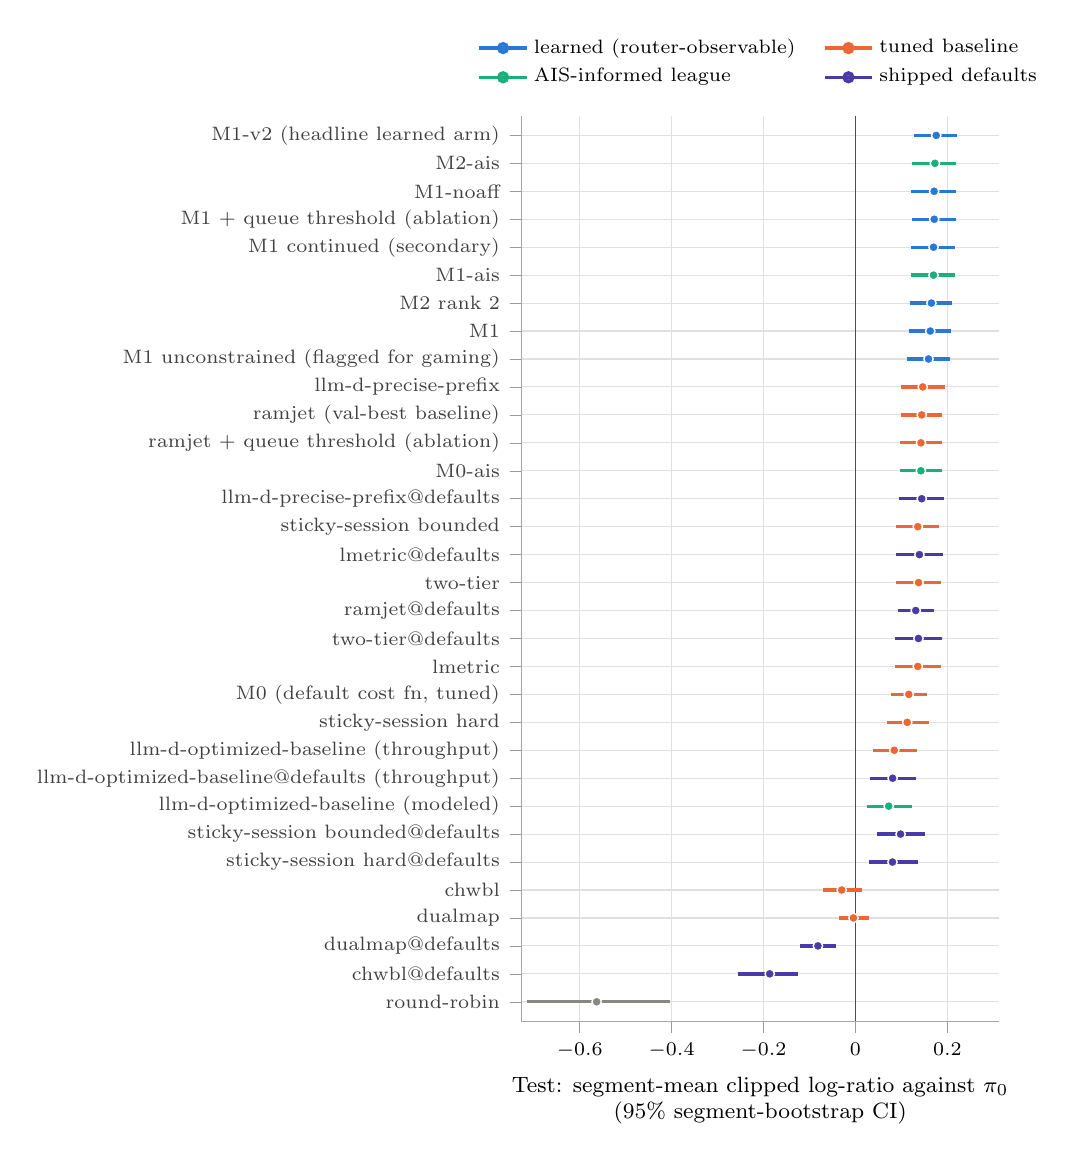
\begin{tikzpicture}
\begin{axis}[
  scale only axis, width=0.5\linewidth, height=11.5cm,
  y dir=reverse, ymin=-0.7, ymax=31.7,
  ytick={0,1,2,3,4,5,6,7,8,9,10,11,12,13,14,15,16,17,18,19,20,21,22,23,24,25,26,27,28,29,30,31}, yticklabels={{M1-v2 (headline learned arm)},{M2-ais},{M1-noaff},{M1 + queue threshold (ablation)},{M1 continued (secondary)},{M1-ais},{M2 rank 2},{M1},{M1 unconstrained (flagged for gaming)},{llm-d-precise-prefix},{ramjet (val-best baseline)},{ramjet + queue threshold (ablation)},{M0-ais},{llm-d-precise-prefix@defaults},{sticky-session bounded},{lmetric@defaults},{two-tier},{ramjet@defaults},{two-tier@defaults},{lmetric},{M0 (default cost fn, tuned)},{sticky-session hard},{llm-d-optimized-baseline (throughput)},{llm-d-optimized-baseline@defaults (throughput)},{llm-d-optimized-baseline (modeled)},{sticky-session bounded@defaults},{sticky-session hard@defaults},{chwbl},{dualmap},{dualmap@defaults},{chwbl@defaults},{round-robin}},
  yticklabel style={font=\scriptsize, text=black!75}, xticklabel style={font=\scriptsize},
  scaled x ticks=false, xticklabel style={/pgf/number format/fixed},
  tick align=outside, tick style={black!40}, axis line style={black!35},
  axis x line*=bottom, axis y line*=left,
  xmajorgrids, ymajorgrids, grid style={black!12, line width=0.4pt},
  enlarge x limits={abs=0.012},
  xmax=0.3,
  xlabel={Test: segment-mean clipped log-ratio against $\piref$\\(95\% segment-bootstrap CI)}, xlabel style={font=\footnotesize, align=center},
  legend style={font=\scriptsize, draw=none, fill=white, fill opacity=0.85, text opacity=1, at={(0.5,1.02)}, anchor=south, legend columns=2, /tikz/every even column/.append style={column sep=8pt}},
  legend cell align=left,
  clip=false,
]
\addlegendimage{color={rgb,255:red,42;green,120;blue,214}, line width=1.2pt, mark=*, mark size=1.6pt}
\addlegendentry{learned (router-observable)}
\addlegendimage{color={rgb,255:red,235;green,104;blue,52}, line width=1.2pt, mark=*, mark size=1.6pt}
\addlegendentry{tuned baseline}
\addlegendimage{color={rgb,255:red,27;green,175;blue,122}, line width=1.2pt, mark=*, mark size=1.6pt}
\addlegendentry{\ais{}-informed league}
\addlegendimage{color={rgb,255:red,74;green,58;blue,167}, line width=1.2pt, mark=*, mark size=1.6pt}
\addlegendentry{shipped defaults}
\draw[black!70, line width=0.6pt] (axis cs:0,-0.7) -- (axis cs:0,31.7);
% row 0: m1v2
\addplot[color={rgb,255:red,42;green,120;blue,214}, line width=1.2pt, forget plot] coordinates {(0.12703656654913123,0) (0.22176766566928766,0)};
\addplot[color={rgb,255:red,42;green,120;blue,214}, only marks, mark=*, mark size=1.7pt, mark options={draw=white, line width=0.5pt}, forget plot] coordinates {(0.17578143769993118,0)};
% row 1: m2ais
\addplot[color={rgb,255:red,27;green,175;blue,122}, line width=1.2pt, forget plot] coordinates {(0.12390968382254673,1) (0.2190776861031586,1)};
\addplot[color={rgb,255:red,27;green,175;blue,122}, only marks, mark=*, mark size=1.7pt, mark options={draw=white, line width=0.5pt}, forget plot] coordinates {(0.17286673166449287,1)};
% row 2: m1noaff
\addplot[color={rgb,255:red,42;green,120;blue,214}, line width=1.2pt, forget plot] coordinates {(0.12181314636266101,2) (0.2178070128886926,2)};
\addplot[color={rgb,255:red,42;green,120;blue,214}, only marks, mark=*, mark size=1.7pt, mark options={draw=white, line width=0.5pt}, forget plot] coordinates {(0.171190484541723,2)};
% row 3: ablam1
\addplot[color={rgb,255:red,42;green,120;blue,214}, line width=1.2pt, forget plot] coordinates {(0.12216696523587754,3) (0.21787594879862668,3)};
\addplot[color={rgb,255:red,42;green,120;blue,214}, only marks, mark=*, mark size=1.7pt, mark options={draw=white, line width=0.5pt}, forget plot] coordinates {(0.17141768706854468,3)};
% row 4: m1cont
\addplot[color={rgb,255:red,42;green,120;blue,214}, line width=1.2pt, forget plot] coordinates {(0.12109149167744096,4) (0.21576375139222648,4)};
\addplot[color={rgb,255:red,42;green,120;blue,214}, only marks, mark=*, mark size=1.7pt, mark options={draw=white, line width=0.5pt}, forget plot] coordinates {(0.169873390601464,4)};
% row 5: m1ais
\addplot[color={rgb,255:red,27;green,175;blue,122}, line width=1.2pt, forget plot] coordinates {(0.12079681370764042,5) (0.21632165247413257,5)};
\addplot[color={rgb,255:red,27;green,175;blue,122}, only marks, mark=*, mark size=1.7pt, mark options={draw=white, line width=0.5pt}, forget plot] coordinates {(0.16985691147737544,5)};
% row 6: m2r2
\addplot[color={rgb,255:red,42;green,120;blue,214}, line width=1.2pt, forget plot] coordinates {(0.11764196543662414,6) (0.21067909813185634,6)};
\addplot[color={rgb,255:red,42;green,120;blue,214}, only marks, mark=*, mark size=1.7pt, mark options={draw=white, line width=0.5pt}, forget plot] coordinates {(0.16533766169352687,6)};
% row 7: m1
\addplot[color={rgb,255:red,42;green,120;blue,214}, line width=1.2pt, forget plot] coordinates {(0.11564640892115144,7) (0.2072323368882717,7)};
\addplot[color={rgb,255:red,42;green,120;blue,214}, only marks, mark=*, mark size=1.7pt, mark options={draw=white, line width=0.5pt}, forget plot] coordinates {(0.16282326060787347,7)};
% row 8: m1u
\addplot[color={rgb,255:red,42;green,120;blue,214}, line width=1.2pt, forget plot] coordinates {(0.11143210946294681,8) (0.20470928733579627,8)};
\addplot[color={rgb,255:red,42;green,120;blue,214}, only marks, mark=*, mark size=1.7pt, mark options={draw=white, line width=0.5pt}, forget plot] coordinates {(0.1589590864709807,8)};
% row 9: llmdpp
\addplot[color={rgb,255:red,235;green,104;blue,52}, line width=1.2pt, forget plot] coordinates {(0.09861310334025862,9) (0.19389557066981786,9)};
\addplot[color={rgb,255:red,235;green,104;blue,52}, only marks, mark=*, mark size=1.7pt, mark options={draw=white, line width=0.5pt}, forget plot] coordinates {(0.14644600247013137,9)};
% row 10: ramjet
\addplot[color={rgb,255:red,235;green,104;blue,52}, line width=1.2pt, forget plot] coordinates {(0.09828279574825906,10) (0.18940257755445838,10)};
\addplot[color={rgb,255:red,235;green,104;blue,52}, only marks, mark=*, mark size=1.7pt, mark options={draw=white, line width=0.5pt}, forget plot] coordinates {(0.14422659924263834,10)};
% row 11: ablabase
\addplot[color={rgb,255:red,235;green,104;blue,52}, line width=1.2pt, forget plot] coordinates {(0.09701337309509567,11) (0.18752162803877784,11)};
\addplot[color={rgb,255:red,235;green,104;blue,52}, only marks, mark=*, mark size=1.7pt, mark options={draw=white, line width=0.5pt}, forget plot] coordinates {(0.14258951638820147,11)};
% row 12: m0ais
\addplot[color={rgb,255:red,27;green,175;blue,122}, line width=1.2pt, forget plot] coordinates {(0.09673094011801839,12) (0.18736256581018823,12)};
\addplot[color={rgb,255:red,27;green,175;blue,122}, only marks, mark=*, mark size=1.7pt, mark options={draw=white, line width=0.5pt}, forget plot] coordinates {(0.14234110495793503,12)};
% row 13: llm-d-precise-prefix@defaults
\addplot[color={rgb,255:red,74;green,58;blue,167}, line width=1.2pt, forget plot] coordinates {(0.09517248828100115,13) (0.19316619122098141,13)};
\addplot[color={rgb,255:red,74;green,58;blue,167}, only marks, mark=*, mark size=1.7pt, mark options={draw=white, line width=0.5pt}, forget plot] coordinates {(0.14420002518899536,13)};
% row 14: stickybounded
\addplot[color={rgb,255:red,235;green,104;blue,52}, line width=1.2pt, forget plot] coordinates {(0.0892680494472722,14) (0.18180551686371837,14)};
\addplot[color={rgb,255:red,235;green,104;blue,52}, only marks, mark=*, mark size=1.7pt, mark options={draw=white, line width=0.5pt}, forget plot] coordinates {(0.1356687801843924,14)};
% row 15: lmetric@defaults
\addplot[color={rgb,255:red,74;green,58;blue,167}, line width=1.2pt, forget plot] coordinates {(0.0888962775650902,15) (0.19013121389356863,15)};
\addplot[color={rgb,255:red,74;green,58;blue,167}, only marks, mark=*, mark size=1.7pt, mark options={draw=white, line width=0.5pt}, forget plot] coordinates {(0.13920811246409123,15)};
% row 16: twotier
\addplot[color={rgb,255:red,235;green,104;blue,52}, line width=1.2pt, forget plot] coordinates {(0.08787299176690117,16) (0.18657524522528626,16)};
\addplot[color={rgb,255:red,235;green,104;blue,52}, only marks, mark=*, mark size=1.7pt, mark options={draw=white, line width=0.5pt}, forget plot] coordinates {(0.13740693013546093,16)};
% row 17: ramjet@defaults
\addplot[color={rgb,255:red,74;green,58;blue,167}, line width=1.2pt, forget plot] coordinates {(0.09256592164675977,17) (0.1706439890179096,17)};
\addplot[color={rgb,255:red,74;green,58;blue,167}, only marks, mark=*, mark size=1.7pt, mark options={draw=white, line width=0.5pt}, forget plot] coordinates {(0.13120578511074651,17)};
% row 18: two-tier@defaults
\addplot[color={rgb,255:red,74;green,58;blue,167}, line width=1.2pt, forget plot] coordinates {(0.08667915681442735,18) (0.18747582618909142,18)};
\addplot[color={rgb,255:red,74;green,58;blue,167}, only marks, mark=*, mark size=1.7pt, mark options={draw=white, line width=0.5pt}, forget plot] coordinates {(0.1370835488619148,18)};
% row 19: lmetric
\addplot[color={rgb,255:red,235;green,104;blue,52}, line width=1.2pt, forget plot] coordinates {(0.08603413756550143,19) (0.18573594528663667,19)};
\addplot[color={rgb,255:red,235;green,104;blue,52}, only marks, mark=*, mark size=1.7pt, mark options={draw=white, line width=0.5pt}, forget plot] coordinates {(0.13559514926145588,19)};
% row 20: m0
\addplot[color={rgb,255:red,235;green,104;blue,52}, line width=1.2pt, forget plot] coordinates {(0.07773044867862913,20) (0.15621326507419445,20)};
\addplot[color={rgb,255:red,235;green,104;blue,52}, only marks, mark=*, mark size=1.7pt, mark options={draw=white, line width=0.5pt}, forget plot] coordinates {(0.11615259593474729,20)};
% row 21: stickyhard
\addplot[color={rgb,255:red,235;green,104;blue,52}, line width=1.2pt, forget plot] coordinates {(0.06816377714898289,21) (0.16085825155500855,21)};
\addplot[color={rgb,255:red,235;green,104;blue,52}, only marks, mark=*, mark size=1.7pt, mark options={draw=white, line width=0.5pt}, forget plot] coordinates {(0.11266423302798644,21)};
% row 22: llmdob
\addplot[color={rgb,255:red,235;green,104;blue,52}, line width=1.2pt, forget plot] coordinates {(0.037722088434720864,22) (0.1341168734355526,22)};
\addplot[color={rgb,255:red,235;green,104;blue,52}, only marks, mark=*, mark size=1.7pt, mark options={draw=white, line width=0.5pt}, forget plot] coordinates {(0.08444506901240169,22)};
% row 23: llm-d-optimized-baseline@throughput
\addplot[color={rgb,255:red,74;green,58;blue,167}, line width=1.2pt, forget plot] coordinates {(0.032531527863121475,23) (0.13140445967972386,23)};
\addplot[color={rgb,255:red,74;green,58;blue,167}, only marks, mark=*, mark size=1.7pt, mark options={draw=white, line width=0.5pt}, forget plot] coordinates {(0.08091673123958297,23)};
% row 24: llmdobm
\addplot[color={rgb,255:red,27;green,175;blue,122}, line width=1.2pt, forget plot] coordinates {(0.02409420705018775,24) (0.12316326800285125,24)};
\addplot[color={rgb,255:red,27;green,175;blue,122}, only marks, mark=*, mark size=1.7pt, mark options={draw=white, line width=0.5pt}, forget plot] coordinates {(0.07239319416774055,24)};
% row 25: sticky-bounded@defaults
\addplot[color={rgb,255:red,74;green,58;blue,167}, line width=1.2pt, forget plot] coordinates {(0.047519933441449176,25) (0.15141698741032308,25)};
\addplot[color={rgb,255:red,74;green,58;blue,167}, only marks, mark=*, mark size=1.7pt, mark options={draw=white, line width=0.5pt}, forget plot] coordinates {(0.09823089855750035,25)};
% row 26: sticky-hard@defaults
\addplot[color={rgb,255:red,74;green,58;blue,167}, line width=1.2pt, forget plot] coordinates {(0.030478380729487182,26) (0.13678912203631782,26)};
\addplot[color={rgb,255:red,74;green,58;blue,167}, only marks, mark=*, mark size=1.7pt, mark options={draw=white, line width=0.5pt}, forget plot] coordinates {(0.08055060851194569,26)};
% row 27: chwbl
\addplot[color={rgb,255:red,235;green,104;blue,52}, line width=1.2pt, forget plot] coordinates {(-0.07107827540927976,27) (0.013233178677833898,27)};
\addplot[color={rgb,255:red,235;green,104;blue,52}, only marks, mark=*, mark size=1.7pt, mark options={draw=white, line width=0.5pt}, forget plot] coordinates {(-0.029918674026883096,27)};
% row 28: dualmap
\addplot[color={rgb,255:red,235;green,104;blue,52}, line width=1.2pt, forget plot] coordinates {(-0.03664970706569164,28) (0.029651301114236972,28)};
\addplot[color={rgb,255:red,235;green,104;blue,52}, only marks, mark=*, mark size=1.7pt, mark options={draw=white, line width=0.5pt}, forget plot] coordinates {(-0.004392614792377874,28)};
% row 29: dualmap@defaults
\addplot[color={rgb,255:red,74;green,58;blue,167}, line width=1.2pt, forget plot] coordinates {(-0.1199719266490455,29) (-0.042838652965060606,29)};
\addplot[color={rgb,255:red,74;green,58;blue,167}, only marks, mark=*, mark size=1.7pt, mark options={draw=white, line width=0.5pt}, forget plot] coordinates {(-0.08165664015863246,29)};
% row 30: chwbl@defaults
\addplot[color={rgb,255:red,74;green,58;blue,167}, line width=1.2pt, forget plot] coordinates {(-0.25565759175765096,30) (-0.12579617818786643,30)};
\addplot[color={rgb,255:red,74;green,58;blue,167}, only marks, mark=*, mark size=1.7pt, mark options={draw=white, line width=0.5pt}, forget plot] coordinates {(-0.18657074945136784,30)};
% row 31: round_robin
\addplot[color={rgb,255:red,137;green,135;blue,129}, line width=1.2pt, forget plot] coordinates {(-0.7147261959541594,31) (-0.40314218613736974,31)};
\addplot[color={rgb,255:red,137;green,135;blue,129}, only marks, mark=*, mark size=1.7pt, mark options={draw=white, line width=0.5pt}, forget plot] coordinates {(-0.5631340198746552,31)};
\end{axis}
\end{tikzpicture}

  % src: CR/report/data/report_data.json comparisons.default.<policy>.all (segment_mean, ci95), drawn by
  %      scripts/make_figures.py with the table labels (formerly fig/leaderboard.png, report figure F3)
  \caption{Every test policy against $\piref$ (60 cells, 12 segments; segment means with 95\%
    segment-bootstrap intervals). Blue: router-observable learned arms; orange: tuned baselines;
    green: the \ais{}-informed league; purple: heuristics at their shipped parameters (suffix
    @defaults); grey: round-robin. The M1 row is also M1 restricted to its default-router start
    (\cref{sec:res-ladder}).}
  % prov: the report's row label for M1 was "M1 (= A12 M1-default-init)"
  \label{fig:leaderboard}
\end{figure}

% =====================================================================================
\subsection{Strata by load mode}
\label{sec:res-strata}

\Cref{tab:strata} breaks the headline down by load mode, worker count, family and transform; the
next two subsections read its worker-count, family and transform rows. Only the first row is a
test; the rest are descriptive, and per-worker-count claims would need Holm's correction, under
which every per-count $p$ is at least 0.070.
% src: CR/report/REPORT.md section 2 ("all Holm-adjusted per-N p >= 0.070")
% prov: the heading was "Strata: load mode, worker count, family and transforms"; sec:res-n and the
%       families subsection read the other strata

\begin{table}[tbp]
  \centering
  \caption{The headline by stratum, M1-v2 minus tuned \policy{ramjet}. One-sided exact
    Wilcoxon $p$ over the stratum's segments; only the first row is a test. Rows marked $\dagger$
    use the within-segment cell bootstrap.}
  \label{tab:strata}
  % GENERATED by scripts/make_tables.py from the report fragment report/data/tables/headline_strata.md.
% Do not edit; regenerate.
{\scriptsize
\begin{adjustbox}{max width=\linewidth}
\begin{tabular}{@{}lrrlrr@{}}
\toprule
Stratum & Cells & Seg. & M1-v2 $-$ ramjet [95\% CI] & Ahead & One-sided $p$ \\
\midrule
\textbf{all (pre-registered test)} & 60 & 12 & $+$0.0316 [$+$0.0150, $+$0.0501] & 10/12 & 0.0017 \\
load mode: open loop & 31 & 8 & $+$0.0281 [$+$0.0032, $+$0.0608] & 5/8 & 0.0742 \\
load mode: closed loop & 15 & 6 & $+$0.0354 [$+$0.0106, $+$0.0633] & 4/6 & 0.0781 \\
load mode: agentic lanes & 14 & 4 & $+$0.0374 [$+$0.0331, $+$0.0411] & 4/4 & 0.0625 \\
$\Nw = 2$ (unseen) & 8 & 6 & $+$0.0382 [$+$0.0138, $+$0.0660] & 6/6 & 0.0156 \\
$\Nw = 4$ (train count) & 13 & 7 & $+$0.0548 [$+$0.0110, $+$0.1085] & 5/7 & 0.0391 \\
$\Nw = 6$ (selection-exposed) & 7 & 6 & $+$0.0296 [$-$0.0004, $+$0.0655] & 3/6 & 0.2188 \\
$\Nw = 8$ (train count) & 17 & 8 & $+$0.0427 [$+$0.0140, $+$0.0788] & 7/8 & 0.0117 \\
$\Nw = 16$ (unseen) & 7 & 6 & $+$0.0288 [$+$0.0096, $+$0.0484] & 5/6 & 0.0312 \\
$\Nw = 32$ (unseen) & 8 & 6 & $+$0.0240 [$+$0.0079, $+$0.0416] & 6/6 & 0.0156 \\
unseen $\Nw$ (2, 16, 32) & 23 & 7 & $+$0.0342 [$+$0.0159, $+$0.0515] & 7/7 & 0.0078 \\
seen $\Nw$ (4, 8) & 30 & 12 & $+$0.0346 [$+$0.0123, $+$0.0610] & 9/12 & 0.0081 \\
transforms beyond train ranges & 10 & 7 & $+$0.0250 [$+$0.0071, $+$0.0443] & 4/7 & 0.1094 \\
family: Mooncake & 25 & 2 & $+$0.0505 [$+$0.0368, $+$0.0645]$^{\dagger}$ & 2/2 & 0.2500 \\
family: FAST25 conversation & 3 & 2 & $+$0.3868 [$+$0.2857, $+$0.4879]$^{\dagger}$ & 2/2 & 0.2500 \\
family: FAST25 synthetic & 3 & 2 & $+$0.0304 [$+$0.0164, $+$0.0443]$^{\dagger}$ & 2/2 & 0.2500 \\
family: sessions & 15 & 4 & $+$0.0001 [$-$0.0001, $+$0.0004] & 2/4 & 0.4375 \\
family: AgentX & 14 & 4 & $+$0.0374 [$+$0.0331, $+$0.0411] & 4/4 & 0.0625 \\
\bottomrule
\end{tabular}
\end{adjustbox}}

\end{table}

M1-v2 leads in all three load modes, by $+0.028$ in open loop, $+0.035$ in closed loop and $+0.037$
in agentic lanes, none significant on its own ($p$ 0.06 to 0.08); \cref{tab:mode} in
\cref{app:tables} gives selected policies by load mode. AgentX ran only in agentic lanes.
% src: generated/strata.tex rows load mode; generated/mode_vs_ramjet.tex, generated/mode_vs_default.tex
%      (tab:mode); CR/cells/{train,val,test}.jsonl (family x load.mode: every AgentX cell, and only
%      AgentX, is in agentic lanes; 8, 4 and 14 cells)

\subsection{Held-out worker counts}
\label{sec:res-n}

\begin{figure}[tbp]
  \centering
  % GENERATED by scripts/make_figures.py from report/data/report_data.json. Do not edit; regenerate.
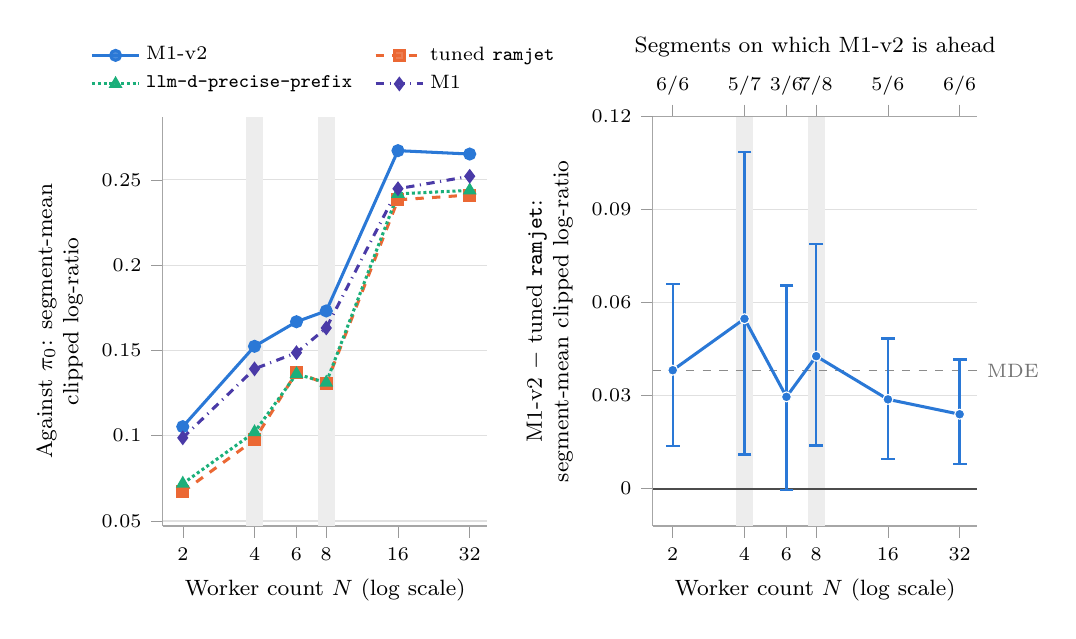
\begin{tikzpicture}
\begin{axis}[
  name=nleft, width=0.34\linewidth, height=5.2cm,
  scale only axis,
  tick label style={font=\scriptsize}, label style={font=\footnotesize, align=center},
  scaled ticks=false, tick label style={/pgf/number format/fixed},
  tick align=outside, tick style={black!40}, axis line style={black!35},
  axis x line*=bottom, axis y line*=left,
  grid style={black!12, line width=0.4pt},
  legend style={font=\scriptsize, draw=none, fill=white, fill opacity=0.85, text opacity=1},
  legend cell align=left,
  xmode=log, log basis x=2, xmin=1.65, xmax=38,
  xtick={2,4,6,8,16,32}, xticklabels={2,4,6,8,16,32}, xminorticks=false,
  xlabel={Worker count $\Nw$ (log scale)},
  ymajorgrids,
  ylabel={Against $\piref$: segment-mean\\clipped log-ratio},
  legend style={at={(0.5,1.03)}, anchor=south, legend columns=2, /tikz/every even column/.append style={column sep=6pt}},
]
\fill[black!7] ({axis cs:3.6807506024995003,0} |- {rel axis cs:0,0}) rectangle ({axis cs:4.346939450104232,0} |- {rel axis cs:0,1});
\fill[black!7] ({axis cs:7.3615012049990005,0} |- {rel axis cs:0,0}) rectangle ({axis cs:8.693878900208464,0} |- {rel axis cs:0,1});
% data: vs_default.m1v2
\addplot[color={rgb,255:red,42;green,120;blue,214}, solid, line width=1.1pt, mark=*, mark size=1.8pt, mark options={solid}] coordinates {(2.0,0.10529501096821288) (4.0,0.15242254036422193) (6.0,0.1668313049122252) (8.0,0.17316070390741592) (16.0,0.2671509076008782) (32.0,0.26516589532107004)};
\addlegendentry{M1-v2}
% data: vs_default.ramjet
\addplot[color={rgb,255:red,235;green,104;blue,52}, dashed, line width=1.1pt, mark=square*, mark size=1.8pt, mark options={solid}] coordinates {(2.0,0.06707443797134567) (4.0,0.09761725816198387) (6.0,0.13720277685467883) (8.0,0.13041631200744147) (16.0,0.2383279917374654) (32.0,0.24114203440810641)};
\addlegendentry{tuned \policy{ramjet}}
% data: vs_default.llmdpp
\addplot[color={rgb,255:red,27;green,175;blue,122}, densely dotted, line width=1.1pt, mark=triangle*, mark size=1.8pt, mark options={solid}] coordinates {(2.0,0.07189553916778706) (4.0,0.10206134188834358) (6.0,0.13618046231011913) (8.0,0.1311275495274687) (16.0,0.24183447602932287) (32.0,0.2438565952246938)};
\addlegendentry{\policy{llm-d-precise-prefix}}
% data: vs_default.m1
\addplot[color={rgb,255:red,74;green,58;blue,167}, dashdotted, line width=1.1pt, mark=diamond*, mark size=1.8pt, mark options={solid}] coordinates {(2.0,0.09875997421164102) (4.0,0.13917749407109334) (6.0,0.14867616361482291) (8.0,0.16317282053987414) (16.0,0.24481944301106787) (32.0,0.25212463174528565)};
\addlegendentry{M1}
\end{axis}
\begin{axis}[
  at={(nleft.south east)}, anchor=south west, xshift=2.1cm,
  width=0.34\linewidth, height=5.2cm, ymin=-0.012, ymax=0.12,
  scale only axis,
  tick label style={font=\scriptsize}, label style={font=\footnotesize, align=center},
  scaled ticks=false, tick label style={/pgf/number format/fixed},
  tick align=outside, tick style={black!40}, axis line style={black!35},
  axis x line*=bottom, axis y line*=left,
  grid style={black!12, line width=0.4pt},
  legend style={font=\scriptsize, draw=none, fill=white, fill opacity=0.85, text opacity=1},
  legend cell align=left,
  xmode=log, log basis x=2, xmin=1.65, xmax=38,
  xtick={2,4,6,8,16,32}, xticklabels={2,4,6,8,16,32}, xminorticks=false,
  xlabel={Worker count $\Nw$ (log scale)},
  ymajorgrids,
  ylabel={M1-v2 $-$ tuned \policy{ramjet}:\\segment-mean clipped log-ratio},
  ytick={0,0.03,0.06,0.09,0.12}, clip=false,
]
\fill[black!7] ({axis cs:3.6807506024995003,0} |- {rel axis cs:0,0}) rectangle ({axis cs:4.346939450104232,0} |- {rel axis cs:0,1});
\fill[black!7] ({axis cs:7.3615012049990005,0} |- {rel axis cs:0,0}) rectangle ({axis cs:8.693878900208464,0} |- {rel axis cs:0,1});
\draw[black!70, line width=0.6pt] ({rel axis cs:0,0} |- {axis cs:0,0.0}) -- ({rel axis cs:1,0} |- {axis cs:0,0.0});
\draw[black!45, line width=0.5pt, dashed] ({rel axis cs:0,0} |- {axis cs:0,0.03815}) -- ({rel axis cs:1,0} |- {axis cs:0,0.03815});
\node[anchor=west, font=\scriptsize, text=black!55] at ({rel axis cs:1,0} |- {axis cs:0,0.03815}) {MDE};
% data: vs_ramjet.ci.N2
\addplot[color={rgb,255:red,42;green,120;blue,214}, line width=0.9pt, mark=-, mark size=2.5pt, forget plot] coordinates {(2.0,0.01379630847680984) (2.0,0.06596507596701744)};
% data: vs_ramjet.ci.N4
\addplot[color={rgb,255:red,42;green,120;blue,214}, line width=0.9pt, mark=-, mark size=2.5pt, forget plot] coordinates {(4.0,0.01103680992682553) (4.0,0.10854519952877277)};
% data: vs_ramjet.ci.N6
\addplot[color={rgb,255:red,42;green,120;blue,214}, line width=0.9pt, mark=-, mark size=2.5pt, forget plot] coordinates {(6.0,-0.00036923336357217357) (6.0,0.06546849679810222)};
% data: vs_ramjet.ci.N8
\addplot[color={rgb,255:red,42;green,120;blue,214}, line width=0.9pt, mark=-, mark size=2.5pt, forget plot] coordinates {(8.0,0.013973978587489277) (8.0,0.07882742248882066)};
% data: vs_ramjet.ci.N16
\addplot[color={rgb,255:red,42;green,120;blue,214}, line width=0.9pt, mark=-, mark size=2.5pt, forget plot] coordinates {(16.0,0.009604036878807847) (16.0,0.048368823083775964)};
% data: vs_ramjet.ci.N32
\addplot[color={rgb,255:red,42;green,120;blue,214}, line width=0.9pt, mark=-, mark size=2.5pt, forget plot] coordinates {(32.0,0.007946861894933812) (32.0,0.041617767312250774)};
% data: vs_ramjet.mean
\addplot[color={rgb,255:red,42;green,120;blue,214}, line width=1.1pt, mark=*, mark size=1.8pt, mark options={draw=white, line width=0.4pt}] coordinates {(2.0,0.03822057299686717) (4.0,0.054805282202238036) (6.0,0.029628528057546417) (8.0,0.04274439189997442) (16.0,0.02882291586341278) (32.0,0.024023860912963633)};
\end{axis}
\begin{axis}[
  at={(nleft.south east)}, anchor=south west, xshift=2.1cm,
  width=0.34\linewidth, height=5.2cm, ymin=-0.012, ymax=0.12,
  scale only axis, xmode=log, log basis x=2, xmin=1.65, xmax=38,
  axis x line*=top, axis y line=none, tick align=outside, tick style={black!40},
  axis line style={black!35}, xminorticks=false,
  tick label style={font=\scriptsize}, label style={font=\footnotesize},
  xtick={2,4,6,8,16,32},
  xticklabels={6/6,5/7,3/6,7/8,5/6,6/6},
  xlabel={Segments on which M1-v2 is ahead},
]
\addplot[draw=none, forget plot] coordinates {(2,0)};
\end{axis}
\end{tikzpicture}

  % src: CR/report/data/report_data.json comparisons.default.<m1v2|ramjet|llmdpp|m1>.N:<n>.segment_mean
  %      and comparisons.ramjet.m1v2.N:<n> (segment_mean, ci95, segments_ahead, segments), drawn by
  %      scripts/make_figures.py (formerly fig/worker_count_extrapolation.png, report figure F2)
  \caption{Worker-count extrapolation on test. Left: segment means
    against $\piref$ by $\Nw$ (intervals in \cref{tab:N-default} in \cref{app:tables}).
    Right: M1-v2 minus tuned \policy{ramjet} by $\Nw$, with 95\% segment-bootstrap intervals and,
    on the top axis, the segments on which M1-v2 is ahead; dashed: the MDE.
    Shaded: the train counts 4 and 8. Each $\Nw$ holds different cells, and loads are matched to
    $\piref$'s knee at each $\Nw$, not to a fixed per-worker rate.}
  \label{fig:n-extrapolation}
\end{figure}

Every learned arm was trained on $\Nw \in \{4, 8\}$ only and runs unchanged at any $\Nw$, because its
utility is per worker and its features are set-size invariant (\cref{sec:set-size}).
\Cref{fig:n-extrapolation} plots the test results by $\Nw$.
\begin{itemize}
  \item \textbf{The margin persists at unseen worker counts.} Over \policy{ramjet} it is positive at
    every $\Nw$: $+0.038$ at $\Nw = 2$, $+0.029$ at 16 and $+0.024$ at 32 (\cref{tab:N-ramjet} in
    \cref{app:tables}). Over
    the 7 segments with cells at unseen counts it is ahead on all 7 ($+0.034$, uncorrected $p$
    0.008); this stratum was not pre-registered as a test.
  \item \textbf{No regression.} The pre-registered no-regression check holds at $\Nw = 2$, 16 and 32
    against both \policy{ramjet} and $\piref$: the lower end of the interval exceeds
    $-\ln 1.005$.
  \item \textbf{Gains over the default grow with $\Nw$} for every cache-aware policy, M1-v2's from
    $+0.105$ at $\Nw = 2$ to $+0.27$ at 16 and 32, but the learned margin over \policy{ramjet} does
    not grow at the unseen large counts.
  \item \textbf{$\Nw = 6$ is selection-exposed} and the weakest stratum: 3 of 6 segments ahead,
    $p$ 0.219.
  \item \textbf{The curve is not a pure $\Nw$ effect.} Each $\Nw$ holds different cells and
    segments, and with loads matched to $\piref$'s knee per $\Nw$ the per-worker load varies 1.2 to
    1.9 times across $\Nw$. A per-worker-matched extrapolation was not run.
\end{itemize}
% src: generated/N_vs_ramjet.tex, generated/strata.tex (unseen_N 7/7, p 0.0078; N:6 3/6, p 0.2188);
%      CR/facts/test_results.json parity_and_no_regression; CR/report/REPORT.md section 4;
%      CR/audits/calibration/independent-rerun-r1.md F3 (1.2-1.9x)
M1-v2's gain rises with cache pressure on the 22 open-loop Mooncake and FAST25 test cells (Spearman
$\rho$ 0.79 against $\piref$, 0.71 against \policy{ramjet}), a descriptive trend confounded with load
level (\cref{app:results}).
% src: CR/report/REPORT.md section 4 ("On the 22 open-loop Mooncake and FAST25 test cells ... Spearman
%      rho 0.79 against default and 0.71 against ramjet ... Pressure is confounded with load level")

\subsection{Families and transforms}

By family (\cref{tab:family-ramjet} in \cref{app:tables}; descriptive, with 2 to 4 segments each),
the margin is largest on the FAST25 conversation cells ($+0.387$), a family no policy was trained on; those three cells carry about 35\% of M1-v2's
cell-mean gain, and their request-count gains ($+0.48$, $+0.49$, $+0.08$) contrast with token-weighted
deltas of $+0.02$, $-0.15$ and $+0.02$ (\cref{sec:gaming}). On Mooncake the lead is $+0.050$, on
AgentX $+0.037$ with all four segments ahead, and on FAST25 synthetic $+0.030$. Sessions sit at
ceiling at the calibrated SLO: every strong policy serves nearly every in-window session request
well, so the four session segments tie. The ten cells with transforms beyond the train ranges show
$+0.025$ with 4 of 7 segments ahead ($p$ 0.109), so generalization to held-out transform values is
not established. \Cref{tab:holdout} in \cref{app:tables} gives selected policies at unseen and seen
worker counts and on the transform cells.
% src: generated/family_vs_ramjet.tex; CR/report/REPORT.md section 3.3 (35%, +0.48/+0.49/+0.08 vs
%      +0.02/-0.15/+0.02); generated/strata.tex (transform_extrapolation +0.0250, 4/7, 0.1094);
%      generated/holdout_vs_{ramjet,default}.tex (tab:holdout columns)

% =====================================================================================
\subsection{The model ladder and the ablations}
\label{sec:res-ladder}

\begin{table}[tbp]
  \centering
  \caption{The model ladder. Val $k_{0..2}$ and Val $k_{3..10}$: mean clipped log-ratio against
    $\piref$ on the selection replicates and on the fresh validation replicates. Test against $\piref$
    is a mean over cells; test against tuned \policy{ramjet} is a segment mean with its 95\% interval
    and one-sided $p$. \Cref{tab:leaderboard-full} in \cref{app:tables} gives the restart and generation at
    which each configuration was selected.}
  % prov: the selected restart and generation moved out of the main text; tab:leaderboard-full has them
  \label{tab:ladder-results}
  % GENERATED by scripts/make_tables.py from the report fragment report/data/tables/ladder.md.
% Do not edit; regenerate.
{\scriptsize
\begin{adjustbox}{max width=\linewidth}
\begin{tabular}{@{}P{0.25\linewidth}rrrlr@{}}
\toprule
Rung & Val $k_{0..2}$ & Val $k_{3..10}$ & Test vs $\piref$ & Test vs ramjet [95\% CI] & $p$ \\
\midrule
M0 & 0.1334 & 0.1326 & $+$0.1102 & $-$0.0281 [$-$0.0439, $-$0.0137] & 0.9993 \\
M1 & 0.1660 & 0.1656 & $+$0.1741 & $+$0.0186 [$+$0.0013, $+$0.0378] & 0.0549 \\
M1 continued ($+$400 evals) & 0.1704 & 0.1672 & $+$0.1811 & $+$0.0256 [$+$0.0090, $+$0.0437] & 0.0212 \\
M2 rank 2 & 0.1688 & 0.1677 & $+$0.1774 & $+$0.0211 [$+$0.0043, $+$0.0406] & 0.0549 \\
M1-noaff & 0.1682 & 0.1692 & $+$0.1821 & $+$0.0270 [$+$0.0109, $+$0.0443] & 0.0134 \\
M1 + queue threshold (ablation) & 0.1690 & 0.1684 & $+$0.1819 & $+$0.0272 [$+$0.0115, $+$0.0444] & 0.0171 \\
M1-v2 & 0.1767 & 0.1783 & $+$0.1877 & $+$0.0316 [$+$0.0150, $+$0.0501] & 0.0017 \\
M1 unconstrained (flagged for gaming) & 0.1636 & n/a & $+$0.1687 & $+$0.0147 [$+$0.0032, $+$0.0284] & 0.0386 \\
M0-ais & 0.1410 & 0.1397 & $+$0.1313 & $-$0.0019 [$-$0.0086, $+$0.0048] & 0.6890 \\
M1-ais & 0.1731 & 0.1718 & $+$0.1810 & $+$0.0256 [$+$0.0113, $+$0.0423] & 0.0012 \\
M2-ais & 0.1751 & 0.1735 & $+$0.1837 & $+$0.0286 [$+$0.0138, $+$0.0458] & 0.0005 \\
\bottomrule
\end{tabular}
\end{adjustbox}}

\end{table}

\Cref{tab:ladder-results} and the rung-to-rung comparisons of \cref{tab:ladder-pairs}
(\cref{app:results}, which also plots the ladder in \cref{fig:ladder}) read as follows.
\begin{itemize}
  \item \textbf{M0 $\to$ M1 is the one clear step.} Learning over the default cost's features beats
    tuning the default cost's knobs: $+0.047$ per segment, 11 of 12 segments ahead.
  \item \textbf{M1 is the sign-constrained re-run.} The first, unconstrained M1 gamed the objective
    (\cref{sec:gaming}); it is reported only as a flagged secondary row, and it is weaker on test.
    % prov: "tier-A M1"
  \item \textbf{M1 $\to$ M2 rank 2: no gain.} The context term adds $+0.0025$ on test (6 of 12
    segments) and does not beat M1 continued for the same added 400 evaluations ($-0.0045$). The
    pre-registered gate for ranks 3 and 4 failed: M2 rank 2 minus the better of M1 and M1 continued
    was $-0.0016$ on validation, against an MDE of 0.038, so ranks 3 and 4 were not run. M3 (nested
    logit) was never built, since this deployment has no nests.
  \item \textbf{M1 $\to$ M1-v2 is the step that passes.} The extended feature set, with log,
    set-relative, interaction and prefill-attention terms, beats M1 by $+0.013$ on 11 of 12 segments
    ($p$ 0.0034). The originally planned M1 and M2 alone do \emph{not} pass against \policy{ramjet}
    on test ($p$ 0.055 each); the passing arm is a redesign made after the pilot, on validation
    evidence (\cref{sec:res-fairness}).
  \item \textbf{The queue-threshold ablation: nothing measurable.} It tunes the router's queue
    threshold jointly with a policy (\cref{sec:ablations}). Against their counterparts without it,
    the learned arm with the threshold is $+0.0015$ ($p$ 0.055, against M1
    continued) and \policy{ramjet} with it is $-0.0016$, and removing the tuned threshold after the
    fact changes their validation scores by $+0.0001$ and $-0.0006$.
  \item \textbf{Session affinity.} M1-noaff, retrained without $\theta_6$, is not worse than M1
    on test ($+0.0084$, $p$ 0.21), and zeroing $\theta_6$ in the selected M1 changes its validation
    score by $-0.0010$. Under router-state lag, M1 minus M1-noaff stays between $-0.008$ and
    $-0.005$, so the hypothesis that affinity gains value as the router's state goes stale is not
    supported. For M1-v2, zeroing $\theta_6$ changes the validation score by $+0.0005$.
    % prov: A15 (M1-noaff)
  \item \textbf{Initialization.} The selected M1 came from the s1 restart, the default router,
    so the registered secondary finalist, M1 restricted to its default start, is the same policy as
    M1.
    % prov: A12, the "M1-default-init" row
    M1-v2 also came from s1; its informed restarts s2 (the behavior clone) and s3 (the faithful LMetric point) reached 0.1609 and
    0.1724 on the selection replicates, against s1's 0.1767.
\end{itemize}
% src: generated/ladder_pairs.tex and generated/ladder.tex; CR/facts/tierBC.json m2_rank3_4_gate
%      (via REPORT section 5: -0.0016 vs MDE 0.038), tier_c_final_i9 (q removed +0.00010 / -0.00064);
%      CR/facts/test_results.json secondary.m1noaff_vs_m1 (+0.008367, p 0.2119), m1_vs_ramjet and
%      m2r2_vs_ramjet (p 0.0549), m1v2_vs_m1 (+0.012958, 11/12, p 0.003418), m1_A12_note;
%      CR/facts/robustness.json a15_affinity_under_lag; CR/audits/final/refute-headline-2.md
%      (M1-v2 theta6 = 0: +0.0005); CR/report/REPORT.md section 5 (restart bests)

% =====================================================================================
\subsection{What M1-v2 learned}
\label{sec:res-coefficients}

The shipped artifact is one policy YAML: \lc{} with \code{feature\_set: v2}, $\temp = 0$,
\code{tie\_break: one\_draw} and the 23 coefficients of \cref{tab:coef-m1v2}. It reads no \ais{}
signal; a decision costs $O(\Nw\dfeat)$ with $\dfeat = 23$. We read the
coefficients through standardized magnitudes and ablations, not raw values: \cref{tab:coef-m1v2}
scales each $\theta_f$ by the feature's within-candidate-set standard deviation on train, so
$\theta_f\,\mathrm{sd}_f$ is the utility change for a typical difference between two candidates. The
anchor, the default cost per request block, has $\theta_0\,\mathrm{sd}_0 = -6.51$
(\cref{fig:coef} in \cref{app:results} plots the nonzero terms).
% src: CR/facts/finalists.json headline.learned.spec; CR/report/REPORT.md section 6 (sd on train from
%      CR/runs/phase2/m1v2/prep.json)
% prov: "Following LR-15" (reading coefficients through standardized magnitudes and ablations)

\begin{table}[tbp]
  \centering
  \caption{M1-v2's coefficients. sd$_f$: pooled within-candidate-set standard deviation
    of feature $f$ on train; constraint: the sign rule of \cref{sec:sign-constraint}.}
  \label{tab:coef-m1v2}
  % GENERATED by scripts/make_tables.py from the report fragment report/data/tables/coef_m1v2.md.
% Do not edit; regenerate.
{\scriptsize
\begin{adjustbox}{max width=\linewidth}
\begin{tabular}{@{}rlrrrl@{}}
\toprule
$f$ & Feature & $\theta_f$ & sd$_f$ & $\theta_f\,\mathrm{sd}_f$ & Constraint \\
\midrule
0 & \code{default\_logit\_scaled} & $-$1 & 6.51 & $-$6.510 & pinned $-$1 \\
1 & \code{overlap\_frac} & $+$5.034 & 0.2561 & $+$1.289 & free \\
2 & \code{new\_prefill\_tokens\_k} & $+$1.275 & 0.3519 & $+$0.449 & free \\
3 & \code{active\_prefill\_tokens\_k} & $-$0.2811 & 1.285 & $-$0.361 & $\leq$ 0 \\
4 & \code{kv\_load\_frac} & $+$0 & 0.08438 & $+$0.000 & $\leq$ 0 \\
5 & \code{active\_requests\_s} & $-$2.146 & 0.06 & $-$0.129 & $\leq$ 0 \\
6 & \code{session\_affinity} & $+$1.391 & 0.3244 & $+$0.451 & free \\
7 & \code{isl\_x\_prefill\_load} & $+$0 & 2.13 & $+$0.000 & $\leq$ 0 \\
8 & \code{log\_ptok} & $+$0 & 1.156 & $+$0.000 & $\leq$ 0 \\
9 & \code{log\_new\_prefill} & $-$0.9276 & 0.8219 & $-$0.762 & free \\
10 & \code{log\_bs} & $+$0 & 0.2708 & $+$0.000 & $\leq$ 0 \\
11 & \code{hash\_home} & $-$1.582 & 0.4668 & $-$0.738 & free \\
12 & \code{kv\_load\_ratio} & $+$0 & 0.2377 & $+$0.000 & $\leq$ 0 \\
13 & \code{active\_prefill\_ratio} & $+$0 & 0.9491 & $+$0.000 & $\leq$ 0 \\
14 & \code{active\_requests\_ratio} & $-$0.348 & 0.2576 & $-$0.090 & $\leq$ 0 \\
15 & \code{kv\_load\_below\_frac} & $+$0 & 0.2817 & $+$0.000 & $\leq$ 0 \\
16 & \code{active\_prefill\_below\_frac} & $-$1.326 & 0.2398 & $-$0.318 & $\leq$ 0 \\
17 & \code{active\_requests\_below\_frac} & $-$2.617 & 0.267 & $-$0.699 & $\leq$ 0 \\
18 & \code{kv\_load\_excess} & $+$0 & 0.05047 & $+$0.000 & $\leq$ 0 \\
19 & \code{active\_prefill\_excess} & $+$0 & 0.9154 & $+$0.000 & $\leq$ 0 \\
20 & \code{active\_requests\_excess} & $-$5.845 & 0.03463 & $-$0.202 & $\leq$ 0 \\
21 & \code{new\_prefill\_x\_requests} & $-$16.79 & 0.1268 & $-$2.128 & $\leq$ 0 \\
22 & \code{prefill\_attn} & $-$0.2967 & 0.2846 & $-$0.084 & free \\
\bottomrule
\end{tabular}
\end{adjustbox}}

\end{table}

\begin{enumerate}
  \item \textbf{The default router plus corrections.} $\theta_0 = -1$ dominates; every learned term
    is a fraction of the anchor's spread.
  \item \textbf{Uncached prefill costs more the busier the worker.} The largest learned term is
    \code{new\_prefill\_x\_requests} ($\theta_{21}\,\mathrm{sd}_{21} = -2.13$). With $\theta_2$, the
    linear weight on uncached prefill is $+1.275 - 0.525 \times$(active requests) per 8K tokens,
    negative on any worker with three or more active requests: uncached work is steered to near-idle
    workers, while cache affinity is kept on lightly loaded ones. Zeroing $\theta_{21}$ costs 0.018 on
    validation (13 of 14 cells worse), and the fairness audit attributes M1-v2's increment over the
    in-class LMetric heuristic to this term.
  \item \textbf{Cache terms reward hits beyond the default's credit.} \code{overlap\_frac}
    ($+1.29$ per sd) and the log of uncached prefill ($-0.76$ per sd) both favor the worker holding
    more of the prompt; the log term rewards near-complete hits most. Zeroing $\theta_1$ alone costs
    only 0.002 on validation: overlap is largely redundant with the anchor and the prefill terms.
  \item \textbf{Rank-like load terms do the balancing.} The set-relative terms
    \code{active\_requests\_below\_frac} ($-0.70$) and \code{active\_prefill\_below\_frac} ($-0.32$),
    with request excess and ratio, outweigh the absolute load terms ($-0.36$ and $-0.13$). LMetric's
    own product terms (\code{log\_ptok}, \code{log\_bs}) are 0 in the selected policy.
  \item \textbf{Session and prefix-home terms are unneeded.} \code{session\_affinity} ($+0.45$) and
    \code{hash\_home} ($-0.74$, a mild avoidance of the prefix's rendezvous pair) can each be zeroed
    with no validation loss ($+0.0005$ and $+0.0010$), so the policy depends on neither session IDs
    nor rendezvous homes.
\end{enumerate}
% src: CR/report/REPORT.md section 6 interpretation (items 1-5); CR/audits/final/refute-headline-2.md
%      (theta21 = 0: -0.0178; theta6 = 0 +0.0005; theta11 = 0 +0.0010)

The \code{v1} arms agree on a simpler structure (\cref{tab:coef-v1} in \cref{app:tables}): a strong extra
overlap credit ($\theta_1\,\mathrm{sd}_1$ of $+4.2$ to $+4.9$) and a strong penalty on active requests
($-2.1$ to $-2.9$) on top of the default. The unconstrained M1 used overlap and request weights about
3.5 to 3.7 times larger and a positive $\theta_7$, the gaming pattern of \cref{sec:gaming}.
% src: CR/report/REPORT.md section 6 ("The v1 arms ...")

% =====================================================================================
\subsection{Robustness}
\label{sec:res-robustness}

\begin{table}[tbp]
  \centering
  \caption{The headline under perturbations and alternative SLOs. ``Nominal $\Ezero$''
    scores timing-perturbed replays against the unperturbed $\Ezero$; ``$\Ezero'$'' uses the
    perturbation-consistent reference (\cref{sec:robustness}). $s$: speedup; $d$: decode speedup.
    $\kendall$-b compares the condition's ranking with the nominal ranking, over the 17 robustness
    finalists for lag and timing and over all 32 non-default policies for SLO variants. The last row
    is the token-weighted secondary metric.}
  \label{tab:robustness}
  % prov: the last row is A19
  % GENERATED by scripts/make_tables.py from the report fragment report/data/tables/robustness.md.
% Do not edit; regenerate.
{\scriptsize
\begin{adjustbox}{max width=\linewidth}
\begin{tabular}{@{}llrrrl@{}}
\toprule
Condition & M1-v2 $-$ ramjet [95\% CI] & Ahead & $p$ & $\kendall$-b & Rank M1-v2 / ramjet \\
\midrule
nominal & $+$0.0316 [$+$0.0150, $+$0.0501] & 10/12 & 0.0017 & 1.000 & 1 / 7 of 17 \\
lag 10 ms & $+$0.0312 [$+$0.0139, $+$0.0508] & 9/12 & 0.0081 & 0.950 & 1 / 7 of 17 \\
lag 50 ms & $+$0.0288 [$+$0.0125, $+$0.0477] & 10/12 & 0.0024 & 0.950 & 1 / 6 of 17 \\
lag 200 ms & $+$0.0304 [$+$0.0135, $+$0.0497] & 9/12 & 0.0061 & 0.917 & 1 / 7 of 17 \\
s0.8 nominal E0 & $+$0.0790 [$+$0.0042, $+$0.1666] & 8/12 & 0.1167 & 0.783 & 1 / 10 of 17 \\
s0.8 E0' & $+$0.0814 [$+$0.0229, $+$0.1511] & 9/12 & 0.0105 & 0.800 & 1 / 10 of 17 \\
s1.2 nominal E0 & $+$0.0151 [$+$0.0064, $+$0.0247] & 10/12 & 0.0081 & 0.950 & 1 / 6 of 17 \\
s1.2 E0' & $+$0.0219 [$+$0.0105, $+$0.0333] & 10/12 & 0.0046 & 0.950 & 1 / 6 of 17 \\
d0.8 nominal E0 & $+$0.0473 [$+$0.0131, $+$0.0872] & 9/12 & 0.0261 & 0.817 & 1 / 7 of 17 \\
d0.8 E0' & $+$0.0391 [$+$0.0145, $+$0.0691] & 10/12 & 0.0024 & 0.917 & 1 / 8 of 17 \\
d1.2 nominal E0 & $+$0.0224 [$+$0.0099, $+$0.0360] & 8/12 & 0.0134 & 0.950 & 1 / 6 of 17 \\
d1.2 E0' & $+$0.0304 [$+$0.0140, $+$0.0477] & 9/12 & 0.0105 & 0.950 & 1 / 6 of 17 \\
SLO scale 0.5 & $+$0.0716 [$-$0.0289, $+$0.1734] & 10/12 & 0.0647 & 0.544 & 1 / 13 of 32 \\
SLO scale 0.75 & $+$0.0353 [$-$0.0015, $+$0.0776] & 8/12 & 0.1167 & 0.907 & 1 / 10 of 32 \\
SLO scale 1.5 & $+$0.0156 [$+$0.0064, $+$0.0256] & 12/12 & 0.0002 & 0.956 & 1 / 10 of 32 \\
SLO scale 2.0 & $+$0.0113 [$+$0.0052, $+$0.0178] & 12/12 & 0.0002 & 0.931 & 2 / 10 of 32 \\
SLO scale 3.0 & $+$0.0120 [$+$0.0048, $+$0.0207] & 12/12 & 0.0002 & 0.919 & 2 / 10 of 32 \\
A14 itl\_only & $+$0.0089 [$+$0.0022, $+$0.0161] & 10/12 & 0.0134 & 0.879 & 1 / 16 of 32 \\
A14 e2e\_only & $+$0.0351 [$+$0.0152, $+$0.0574] & 11/12 & 0.0012 & 0.988 & 1 / 11 of 32 \\
A14 ttft\_len\_itl & $+$0.0134 [$+$0.0046, $+$0.0227] & 10/12 & 0.0105 & 0.847 & 1 / 10 of 32 \\
A14 abs\_e2e\_itl & $+$0.0189 [$+$0.0082, $+$0.0303] & 10/12 & 0.0061 & 0.891 & 1 / 15 of 32 \\
A19 good tokens (secondary) & $-$0.0092 [$-$0.0645, $+$0.0244] & 10/12 & 0.0320 & n/a & n/a \\
\bottomrule
\end{tabular}
\end{adjustbox}}

\end{table}

\Cref{tab:robustness} answers whether the ranking survives changes training never saw
(\cref{fig:robustness} in \cref{app:results} plots it).\footnote{The measurement window matters
  little: starting the window 25\% or 50\% later gives $+0.0345$ and $+0.0297$; halving or doubling
  the warm-up, or a common completion window, leaves the result unchanged on the same cells.}
% src (footnote): CR/audits/final/refute-headline-3.md (window +25%/+50%)
\begin{itemize}
  \item \textbf{Router-state lag.} At 10, 50 and \SI{200}{ms} the lead is $+0.031$, $+0.029$ and
    $+0.030$ ($p \le 0.0081$), M1-v2 stays first among the 17 robustness finalists, and the ranking's
    $\kendall$-b is 0.92 to 0.95. At lag 0 the patched replay reproduces the unpatched one per request
    (\cref{app:results}). Beyond the registered range, on validation only, \SI{1000}{ms} gives
    $+0.033$ against $+0.029$ at 0: the baselines lose more to staleness than M1-v2 does.
  \item \textbf{Engine timing.} The sign holds under speedup and decode speedup of 0.8 and 1.2, on
    both references, and with the ITL bound also rescaled the lead is $+0.022$ to $+0.080$
    ($p \le 0.0081$). Speedup 0.8 on the nominal $\Ezero$ is not significant ($p$ 0.117), a degenerate
    scoring in which no zero-reuse AgentX request can be good. The spread across conditions (0.060,
    set by speedup 0.8) exceeds the nominal effect, so by the reading rule of \cref{sec:robustness}
    the direction is robust and the magnitude is perturbation-dependent.
    % prov: LR-14 (the reading rule)
  \item \textbf{SLO scale.} The sign is positive at every scale; significance holds at 1 to 3 and is
    lost at 0.75 and 0.5. At 0.75 the four session segments reverse ($-0.014$ to $-0.042$), as they do
    at speedup 0.8 on the nominal reference, so ``sessions at ceiling'' holds only where the SLO does
    not bind. At 0.5 the scaled slowdown bound falls below 1 for AgentX, so only cache hits can be
    good there.
  \item \textbf{SLO definition (registered before the test pass).} M1-v2 ranks first under all
    four alternative definitions of a good request, and the ranking's $\kendall$-b against the
    trained SLO is 0.85 to 0.99: ITL only $+0.0089$ ($p$ 0.013), slowdown only $+0.035$ ($p$ 0.0012),
    length-scaled TTFT plus ITL $+0.013$ ($p$ 0.0105), absolute end-to-end plus ITL $+0.019$
    ($p$ 0.0061).
    % prov: A14
  \item \textbf{Simulator model.} On validation, four audit-only changes to \aisim{}'s pricing of
    mixed prefill and decode passes, which act on M1-v2's concentration mechanism, keep the lead
    between $+0.0268$ and $+0.0291$ against $+0.0290$; they bracket fidelity errors, are not
    measurements of reality and do not cover FAST25, a test-only family (\cref{app:results}).
    % src (pricing owner): CR/facts/UPSTREAM_FOLLOWUPS.md #17; appendix-caveats.tex row 13
  \item \textbf{Herding guards.} Run as variants of M1 (they were registered before M1-v2 won),
    neither a positive temperature nor restricting candidates to the prefix's hash-home pair helps,
    and no herding failure of the argmax appeared under the tested lags in replay
    (\cref{app:results}).
    % src: generated/tau_hashhome.tex; CR/facts/robustness.json m1_lr14_variants; CR/report/REPORT.md
    %      section 7.2
\end{itemize}
% src: generated/robustness.tex; CR/facts/robustness.json (conditions, lag0_identity_lag_build_vs_tuning_build,
%      lr14_summary); CR/audits/final/refute-headline-3.md (lag0 448/448; lag 1000 ms val +0.0333 vs
%      +0.0290; consistent timing SLO +0.022..+0.080, p <= 0.0081; window +25%/+50%; simulator model
%      variants); CR/report/REPORT.md section 7.1

% =====================================================================================
\subsection{The \ais{}-informed league}
\label{sec:res-ais-summary}

% src: generated/ladder_pairs.tex (M2-ais - M1-v2 -0.0029, 3/12; M0-ais - M0 +0.0262);
%      CR/facts/robustness.json execution.ais_league; CR/audits/final/completeness.md F2;
%      CR/facts/UPSTREAM_FOLLOWUPS.md #15
% prov: A16 (the AIS league); the full section moved to app:ais-league, which keeps sec:res-ais
The \ais{}-informed league, whose policies may read \ais{} estimates at runtime and so can never
become the headline, adds nothing at the learned level: M2-ais trails M1-v2 by 0.0029 (3 of 12 segments ahead),
although the \ais{} load model helps the default cost ($+0.026$). The league has no lag or timing
robustness evidence and is not portable as is (\cref{sec:res-ais}).

% =====================================================================================
\subsection{Scope: the in-class heuristic and asymmetric iteration}
\label{sec:res-fairness}

Equal footing was verified from the raw tuning histories by two auditors: every tuned policy, learned
or baseline, ran three restarts of 400 evaluations with the same cells, replicates, validation
schedule, objective and reference, and the splits share no trace files. The fairness audit then found
a gap that equal budgets do not close. By design the baseline pool holds the branch's
ports as implemented, and the \policy{lmetric} port as evaluated lacks LMetric's queued-prefill term
(\cref{sec:ports}). Faithful LMetric is inside M1-v2's hypothesis class, and M1-v2's restart s3
started from default plus 20.7 times the faithful LMetric point. \Cref{tab:fairness} shows what that
heuristic does on its own.
% src: CR/audits/final/refute-headline-2.md (equal footing PASS: 48 runs, one budget signature;
%      no leakage), F1; CR/facts/fairness_in_class_heuristic.json; CR/facts/test_results.json
%      report_must_state MS-RH2-F1-table, MS-RH2-F1-increment
% prov: "By design" was "By operator decision"

\begin{table}[tbp]
  \centering\small
  \caption{The in-class heuristic. \emph{Auditor diagnostic, not pre-registered, never used for
    selection; train and validation only, the test split was not evaluated.} Mean clipped
    log-ratio against $\piref$; the last column is the margin over \policy{ramjet} on the fresh
    validation replicates, per cell and per segment.}
  \label{tab:fairness}
  % src: CR/facts/fairness_in_class_heuristic.json (via CR/report/REPORT.md section 9 table, which
  %      re-derives every value from the cache: runs/final-fix/scripts/verify_fairness.py)
  \begin{adjustbox}{max width=\linewidth}
  \begin{tabular}{@{}P{0.38\linewidth}rrrl@{}}
    \toprule
    Policy (tuning) & Train $k_{0..1}$ & Val $k_{0..2}$ & Val $k_{3..10}$ & vs ramjet on $k_{3..10}$: cell / segment \\
    \midrule
    M1-v2 ($3 \times 400$ evaluations) & 0.1851 & 0.1767 & \textbf{0.1783} & $+0.0372$ / $+0.0290$ (5 of 6) \\
    default $+$ $10\times$ faithful LMetric (8 train evaluations) & 0.1566 & 0.1609 & \textbf{0.1609} & $+0.0197$ / $+0.0179$ (4 of 6) \\
    M1-v2's s3 start, $c = 20.7$ (untuned) & 0.1566 & 0.1596 & \textbf{0.1612} & $+0.0200$ / $+0.0190$ (6 of 6) \\
    faithful LMetric alone (untuned) & 0.1466 & 0.1493 & \textbf{0.1490} & $+0.0079$ / $+0.0110$ (6 of 6) \\
    \policy{ramjet} (best of 11 tuned baselines, $3 \times 400$) & 0.1435 & 0.1420 & \textbf{0.1411} & --- \\
    \bottomrule
  \end{tabular}
  \end{adjustbox}
\end{table}

\begin{itemize}
  \item \textbf{Faithful LMetric beats every tuned baseline untuned,} on the selection replicates
    (0.1493 against at most 0.1423) and on the fresh ones (0.1490 against 0.1411).
  \item \textbf{Most of the margin is the heuristic.} Default plus faithful LMetric reproduces 53 to
    66\% of M1-v2's fresh-validation margin over \policy{ramjet}.
  \item \textbf{The learned increment} over it is about $+0.011$ per segment (standard error 0.0065,
    5 of 6 segments; $+0.017$ per cell), about 0.29 of the MDE, and it \emph{was not measured on
    test}; it sits mostly on one Mooncake validation segment.
  \item \textbf{Follow-up.} A pre-registered comparison with faithful LMetric and an SMetric-style
    baseline, each tuned with the equal budget and evaluated on fresh segments or on live runs over
    cells outside the frozen test set, has not been run and is not part of this paper.
    (The live runs of \cref{sec:live} used frozen test cells and so cannot serve it.)
  \item \textbf{The port has changed since.} After this study froze its results, the
    \policy{lmetric} port in ai-dynamo/dynamo\#15450 was fixed to count the worker's queued prefill,
    so it now scores the same product as the faithful LMetric rows above, plus its hot-spot filter.
    The fixed port was not evaluated, and the diagnostic is unchanged: its faithful rows are points
    of M1-v2's class, not the port, the tuned baselines and every \policy{lmetric} number in this
    paper are from the port before the fix, and the follow-up above has still not been run.
    % src: CR/CONTRACT.md A21; CR/facts/fairness_in_class_heuristic.json policies.lmetric_faithful
    %      (learned-choice v2, theta = -(e_log_ptok + e_log_bs): argmin (active_prefill + new_prefill) x
    %      (active_requests + 1))
\end{itemize}
% src: CR/facts/fairness_in_class_heuristic.json; CR/report/REPORT.md section 9 (increment +0.0110 per
%      segment, SE 0.0065, 5/6; cell +0.0174; mostly Mooncake w1 +0.044); CR/audits/final/fix.md (escalation)

\paragraph{Asymmetric iteration.}
The learned side was redesigned on validation evidence: multi-start initialization, the sign
constraints, and M1-v2 itself, which was written to target the pilot's weakest family, plus M2,
M1-noaff and the queue-threshold arm. The baseline side gained one arm and no new heuristic types.
Selection among the five learned arms used the same fresh-validation rule as the baselines, and the
test pass was single, so the headline $p$-value is valid for the selected arm; but the originally
planned M1 and M2 do not pass on test. Two registration choices (excluding M1 continued from the
headline candidates and including the queue-threshold \policy{ramjet} in the baseline pool) cannot be
shown to predate the fresh-validation results; both were outcome-neutral on those values, and we do
not claim strict pre-registration for them.
% src: CR/audits/final/refute-headline-2.md F2; CR/audits/final/completeness.md F5;
%      CR/audits/final/refute-headline-1.md F6; CR/report/REPORT.md section 9 ("Registration timing")

% SPDX-FileCopyrightText: Copyright (c) 2026 NVIDIA CORPORATION & AFFILIATES. All rights reserved.
% SPDX-License-Identifier: Apache-2.0
%
% ROLE: the objective-gaming finding (phase-2 midpoint), its sign-constraint remedy and what remains:
%   concentration of short requests, the long-prompt trade, the A19 token-weighted secondary metric
%   and the other secondary metrics.
% EVIDENCE: CR/audits/phase2-mid/{gaming-concentration,sim-exploitation,fix}.md; CR/facts/
%   {phase2_mid_fix,tierBC,test_results,secondary_metrics_test}.json; CR/report/REPORT.md sections
%   10.1-10.3; generated/{lr13_flags,isl_buckets,secondary_vs_ramjet}.tex.
% STATUS: final for the simulation results.

\section{Objective gaming, concentration and long prompts}
\label{sec:gaming}

The objective counts good requests. A request is good or not, whatever its size, so a policy can
raise the count by serving many short requests well at the expense of a few long ones. This section
reports how the search exploited that, how the exploit was removed, and what remains in the
headline policy.

\subsection{The finding: a sacrificial worker}
\label{sec:gaming-finding}

At the phase-2 midpoint an adversarial audit replayed the selected tier-A M1 (unconstrained) and
every contender on the 14 validation cells with its own scorer, and examined each request.
% src: CR/audits/phase2-mid/gaming-concentration.md (882 replays, 0 errors; own scorer matches the
%      harness on 882/882; results tables)
\begin{itemize}
  \item \textbf{Concentration.} M1 sent more than the cap $\min(2/\Nw, 1/\Nw + 0.25)$ of a cell's
    requests to one worker on 4 of the 5 Mooncake validation cells (up to 0.454 against a cap of
    0.333), while every contender baseline stayed within the cap. The concentration was in requests,
    not work: the hottest worker's share of prefill tokens stayed near $1/\Nw$. It carried one
    shared-prefix group, and the extra concentration bought almost no cache: on the violating cells,
    M1's prefix reuse was at most 0.0065 above the best within-cap baseline and below it on two.
  \item \textbf{A worker of lost requests.} On the heaviest Mooncake cell, in every replicate, M1 left
    one worker receiving only 14 to 16 in-window requests, all very long (median prompt 98K to 100K
    tokens), and none of them good, while the hot workers served 519 to \num{1014} mostly short,
    cached requests at 0.90 to 0.99 good. These long requests share only one 512-token block, so
    stacking them has no cache rationale, and they were not doomed: $\piref$, \policy{ramjet} and M0
    served every request of 60K tokens or more well on that cell, M1 only 42.5\%.
  \item \textbf{Mechanism: load attracted long requests.} When a request of 60K tokens or more
    arrived, M1 sent it to the worker with the most outstanding prefill 58\% of the time, against a
    chance rate of 12.5\% and 0 to 2\% for the baselines. The selected coefficients predict this:
    with $\theta_7 > 0$ (the product of prompt length and active prefill), the net coefficient on a
    worker's active prefill turns positive for prompts above about 77K tokens, so a long request is
    drawn to a worker that is already busy. Setting $\theta_7 = 0$ alone removed the lost-requests
    worker on all three restarts and brought the long requests back to 0.94 to 1.00 good.
  \item \textbf{Not starvation in the long-wait sense.} M1's share of requests slower than three
    times the slowdown bound was below every baseline's; the sacrificed requests missed narrowly
    (median slowdown 1.13 times the bound).
\end{itemize}
% src: CR/audits/phase2-mid/gaming-concentration.md "Concentration" (4 of 5 cells; 0.454 at
%      islu1.25-n6-closed-L2, cap 0.333; prefill share 0.146 vs 0.125 at N8; reuse at most +0.0065),
%      "Sacrifice and starvation" (k0 0/16, k1 0/14, k2 0/15; median ISL 98-100K; 519-1,014 at
%      0.90-0.99; group 14 shares 1 block; ISL >= 60K good 0.425 vs 1.000), "Mechanism" (0.580 vs 0.125;
%      default 0.7-2.2%, ramjet 0-0.7%; threshold about 77K; theta7 = 0 -> 0.943, 1.000, 1.000),
%      "No starvation" (median slowdown of a giant 1.13 S)
The audit's verdict was objective gaming, which triggered the remedy registered in advance
(Amendment A11.2). Black-box search exploiting a gap in its objective is a known pattern
\citep{lehman2020creativity}, and a binary per-request goodput invites exactly this trade
\citep{wang2024slo}; a router tuned by an evolution strategy on tail TTFT alone sent all traffic to
one replica \citep{toniolo2026gorgo}. A companion audit of simulator exploitation found the
long-prompt sacrifice stable across 26 perturbations of timing, lag, window and SLO, so it is a
property of the policy, not of a fragile corner of the simulator.
% src: CR/audits/phase2-mid/gaming-concentration.md F1 ("A11.2 decision: GAMING");
%      CR/audits/phase2-mid/sim-exploitation.md F1 (via CR/facts/STATE.md: "Mooncake long-ISL sacrifice
%      is stable, not sim-fragile ... in 12/12 conditions"; "26 counterfactuals")

\subsection{The remedy: load must not attract}
\label{sec:gaming-remedy}

The remedy re-ran all three M1 restarts with $\theta_3, \theta_4, \theta_5, \theta_7 \le 0$, at the
same budget, seeds and starting points (\cref{sec:sign-constraint}), and every later learned arm used
the same rule. A re-audit with the audit's own scripts, unchanged, then compared the constrained M1
with the unconstrained one.
\begin{itemize}
  \item \textbf{Removed.} No Mooncake validation cell has a lost-requests worker (the unconstrained
    M1 had one per replicate on two cells); requests of 60K tokens or more are 0.92 to 1.00 good
    (0.425 to 0.966 before); the share of them sent to the worker with the most outstanding prefill
    fell to 0.07 to 0.20, near or below chance (0.37 to 0.58 before).
  \item \textbf{Remaining.} The constrained M1 still exceeds the share cap on 4 of 5 Mooncake cells,
    at higher shares than before (0.56 against a cap of 0.25 on the two cells at $\Nw = 8$), and still
    segregates by prompt length: the normalized mutual information between worker and prompt-length
    quartile is 0.21 to 0.23 at $\Nw = 8$, against at most 0.095 for the contender baselines. Long
    prompts still lose: on the heaviest cell 0.826 of prompts of 32K tokens or more are good, against
    0.995 under $\piref$ and 0.963 under \policy{ramjet}, and 65 to 69\% of the requests that turn
    bad against $\piref$ fall in the top prompt-length quartile.
\end{itemize}
% src: CR/audits/phase2-mid/fix.md "Re-audit result" (dump workers 0; ISL >= 60K good 0.920-1.000 vs
%      0.425-0.966; giants to max-prefill worker 0.071-0.203 vs 0.370-0.580, chance 0.125-0.25; shares
%      0.558/0.567 vs cap 0.25; NMI 0.211/0.228, contenders <= 0.095; >= 32K good 0.826 vs 0.995/0.963;
%      65-69% of good-to-bad in the top quartile)
The sign constraint removed the pathological mechanism, a worker that collects long requests it
cannot serve, but not the underlying trade: short cached requests are packed onto a hot worker and
long prompts compete for the rest. By the outcome rule registered with the remedy, the flags are
reported on every learned row and are never a reason to retune or reselect; retuning under a
size-aware objective is a design decision for the operator. The operator kept the request-count
objective, headline and selection unchanged and added one token-weighted secondary metric (Amendment
A19, \cref{sec:a19}). The same re-audit on the later learned arms (M2, M1-v2, M1-noaff and M1
continued) flagged each on 3 or 4 Mooncake validation cells, with no lost-requests worker for any.
% src: CR/facts/phase2_mid_fix.json preregistration.gaming_reaudit (outcome rule); CR/CONTRACT.md A19;
%      CR/facts/tierBC.json decisions.tier_b_reaudit_i9 (m2r2, m1v2, m1noaff flagged on 4 cells,
%      m1cont 3; "No dump worker for any arm")

\subsection{Concentration on test}
\label{sec:gaming-test}

\Cref{tab:lr13} applies the window-basis guards to every test policy. Every learned arm concentrates
and segregates by prompt length far more than the strong baselines: M1-v2 exceeds the share cap on 24
of 60 test cells, against 5 for \policy{ramjet} and 0 for $\piref$, and its worker assignment carries
information about prompt length on 19 cells, against 5. A worker with no good request (``dump
worker'' in the table) appears on 5 of M1-v2's cells and 3 of \policy{ramjet}'s; the unconstrained M1
has 9, and more long-request flags than M1-v2 (20, 20 and 15 cells against 11, 10 and 10).
% src: generated/lr13_flags.tex (from report/data/tables/lr13_flags.md; CR/facts/test_results.json lr13_flags)

\begin{table}[tbp]
  \centering
  \caption{Concentration and long-request flags on test, counts of the 60 test cells (generated).
    Share $>$ cap: the window-basis largest worker request share exceeds
    $\min(2/\Nw, 1/\Nw + 0.25)$. NMI: normalized mutual information between worker and prompt-length
    quartile above 0.10. $\geq$32K, $\geq$64K, top decile: the good fraction of those prompts is more
    than 0.05 below $\piref$'s. Dump worker: a worker with 0\% good in-window requests. Last column:
    mean over cells of the smallest per-worker good fraction.}
  \label{tab:lr13}
  % GENERATED by scripts/make_tables.py from the report fragment report/data/tables/lr13_flags.md.
% Do not edit; regenerate.
{\scriptsize
\begin{adjustbox}{max width=\linewidth}
\begin{tabular}{@{}P{0.36\linewidth}rrrrrrr@{}}
\toprule
Policy & Share $>$ cap & NMI $> 0.10$ & $\geq$32K & $\geq$64K & Top decile & Dump worker & Min worker good \\
\midrule
M1-v2 (headline learned arm) & 24 & 19 & 11 & 10 & 10 & 5 & 0.841 \\
M2-ais & 22 & 20 & 13 & 7 & 10 & 3 & 0.844 \\
M1-noaff & 23 & 19 & 11 & 6 & 11 & 2 & 0.836 \\
M1 + queue threshold (abl. a) & 24 & 19 & 12 & 7 & 11 & 3 & 0.840 \\
M1 continued (secondary) & 23 & 18 & 14 & 8 & 11 & 2 & 0.830 \\
M1-ais & 25 & 22 & 11 & 6 & 10 & 5 & 0.837 \\
M2 rank 2 & 23 & 20 & 11 & 6 & 10 & 3 & 0.832 \\
M1 (= A12 M1-default-init) & 21 & 20 & 11 & 7 & 10 & 1 & 0.834 \\
M1 unconstrained (gaming-flagged) & 20 & 20 & 20 & 20 & 15 & 9 & 0.753 \\
llm-d-precise-prefix & 5 & 6 & 6 & 4 & 5 & 2 & 0.845 \\
ramjet (val-best baseline) & 5 & 5 & 1 & 0 & 3 & 3 & 0.849 \\
ramjet + queue threshold (abl. a) & 5 & 5 & 0 & 0 & 1 & 2 & 0.852 \\
M0-ais & 5 & 5 & 3 & 1 & 2 & 2 & 0.850 \\
llm-d-precise-prefix@defaults & 6 & 8 & 4 & 2 & 4 & 3 & 0.840 \\
sticky-session bounded & 3 & 3 & 2 & 0 & 4 & 2 & 0.850 \\
lmetric@defaults & 2 & 2 & 5 & 3 & 5 & 4 & 0.835 \\
two-tier & 3 & 1 & 5 & 1 & 4 & 3 & 0.832 \\
ramjet@defaults & 3 & 2 & 2 & 1 & 3 & 2 & 0.854 \\
two-tier@defaults & 4 & 5 & 3 & 2 & 3 & 3 & 0.827 \\
lmetric (port) & 2 & 0 & 5 & 3 & 5 & 3 & 0.837 \\
M0 (default cost fn, tuned) & 3 & 3 & 2 & 1 & 3 & 1 & 0.848 \\
sticky-session hard & 0 & 0 & 3 & 6 & 11 & 1 & 0.843 \\
llm-d-optimized-baseline (throughput) & 3 & 4 & 2 & 4 & 9 & 3 & 0.799 \\
llm-d-optimized-baseline@throughput & 5 & 5 & 1 & 3 & 11 & 2 & 0.793 \\
llm-d-optimized-baseline (modeled) & 5 & 5 & 15 & 8 & 19 & 2 & 0.792 \\
sticky-bounded@defaults & 0 & 0 & 1 & 0 & 2 & 1 & 0.800 \\
sticky-hard@defaults & 0 & 0 & 1 & 6 & 10 & 1 & 0.785 \\
chwbl & 14 & 7 & 14 & 18 & 27 & 0 & 0.724 \\
dualmap & 14 & 16 & 11 & 11 & 31 & 3 & 0.646 \\
dualmap@defaults & 13 & 22 & 18 & 19 & 33 & 4 & 0.542 \\
chwbl@defaults & 14 & 16 & 25 & 22 & 44 & 1 & 0.555 \\
round\_robin & 0 & 0 & 39 & 30 & 57 & 0 & 0.419 \\
default@defaults (reference) & 0 & 0 & 0 & 0 & 0 & 0 & 0.755 \\
\bottomrule
\end{tabular}
\end{adjustbox}}

\end{table}

The engine state stays inside the simulator's measured range. On Mooncake, M1-v2's hottest worker
carries 1.85 times the per-worker mean of in-flight requests (\policy{ramjet} 1.04, $\piref$ 1.18), and
2.21 and 1.67 times on FAST25 conversation and synthetic. Peak in-flight requests are 59 and 65, inside
\ais{}'s measured vLLM decode grid and far below \code{max\_num\_seqs}, so the concentration does not
push the engine into the performance model's extrapolation. M1-v2 also shows no preference for pairing
short prompts with long prefill chunks, the mixed-batch pricing artifact a search could exploit
(caveat 13 in \cref{tab:caveats}), and has fewer requests that finish below their uncontended latency
than \policy{ramjet} or \policy{llm-d-precise-prefix}.
% src: CR/report/REPORT.md section 10.1 "Engine state" (from CR/audits/final/refute-headline-3.md section 6:
%      1.85x, 1.04, 1.18; 2.21x, 1.67x; peak 59 and 65; decode grid up to batch 2,048, context 131,071;
%      max_num_seqs 1,024; fewer below-E0 rows; closes UPSTREAM_FOLLOWUPS #17's exploit check)

\subsection{Where the gain comes from: prompt length}
\label{sec:gaming-isl}

\begin{table}[tbp]
  \centering
  \caption{Good fraction and TTFT by prompt length on test (generated; descriptive, computed after
    the test pass from its records). Good-fraction differences in percentage points, with the number
    of segments on which M1-v2 is higher; TTFT p90 as a segment-mean log-ratio.}
  \label{tab:isl}
  % GENERATED by scripts/make_tables.py from the report fragment report/data/tables/isl_buckets.md.
% Do not edit; regenerate.
{\scriptsize
\begin{adjustbox}{max width=\linewidth}
\begin{tabular}{@{}lrrrrr@{}}
\toprule
Prompt tokens & Good frac.\ M1-v2 $-$ ramjet (pp) & Seg.\ higher & Good frac.\ ramjet $-$ $\piref$ (pp) & TTFT p90 log-ratio, M1-v2 vs ramjet & Seg.\ higher \\
\midrule
0-2048 & $+$4.3 & 8/12 & $+$19.4 & $+$0.027 & 6/12 \\
2048-8192 & $+$4.3 & 8/12 & $+$16.6 & $-$0.012 & 5/12 \\
8192-32768 & $-$1.7 & 7/12 & $+$7.2 & $+$0.029 & 10/12 \\
32768-65536 & $-$3.8 & 5/10 & $+$4.5 & $+$0.135 & 11/12 \\
65536- & $-$3.7 & 4/8 & $+$1.1 & $+$0.033 & 4/8 \\
\bottomrule
\end{tabular}
\end{adjustbox}}

\end{table}

\begin{figure}[tbp]
  \centering
  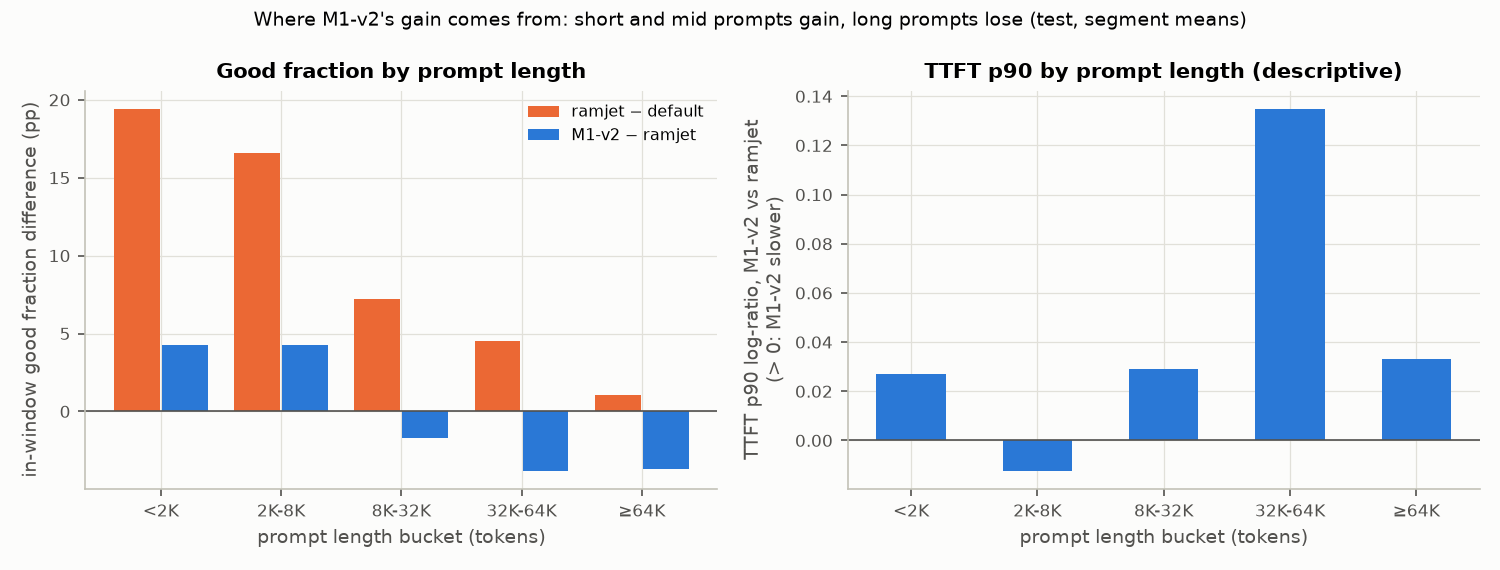
\includegraphics[width=\linewidth]{isl_buckets}
  \caption{Where M1-v2's gain comes from (copied from the final report). Left: in-window good fraction
    by prompt length, \policy{ramjet} minus $\piref$ (orange) and M1-v2 minus \policy{ramjet} (blue).
    Right: TTFT p90 log-ratio of M1-v2 against \policy{ramjet}.}
  \label{fig:isl}
\end{figure}

\Cref{tab:isl,fig:isl} show the trade the request-count objective rewards.
\begin{itemize}
  \item \textbf{The gain sits in short and mid prompts.} M1-v2 gains 4.3 points of good fraction
    below 8K tokens and gives up 1.7 to 3.8 points at 8K and above.
  \item \textbf{Long prompts wait longer than under \policy{ramjet}.} Its TTFT p90 for 32K to 64K
    prompts is higher on 11 of 12 segments (log-ratio $+0.135$, a factor of 1.145); counting only
    records with at least 20 such prompts in both arms it is $+0.169$ on 8 of 8. That is about the
    default router's own long-prompt TTFT ($-0.011$ against $\piref$), while \policy{ramjet} is
    $-0.180$ below $\piref$ there. Overall TTFT is on par with \policy{ramjet}: p50 $+0.006$, p90
    $-0.002$, p99 $-0.082$.
\end{itemize}
% src: CR/facts/test_results.json report_must_state MS-F1-ttft (p50 +0.006, p90 -0.002, p99 -0.082;
%      32K-64K +0.135, 11/12; filtered +0.169, 8/8; vs default -0.011; ramjet -0.180), MS-F1-goodfrac-by-isl

\subsection{Token-weighted goodput (A19)}
\label{sec:a19}

Amendment A19 added one secondary metric, registered before it was computed: the headline pipeline
with each good in-window request weighted by its prompt plus output tokens, on exactly the requests
and good rule that produce the headline's goodput. It never selects a policy or decides the headline.
Against \policy{ramjet}, M1-v2's token-weighted goodput is mixed: segment mean $-0.0092$, interval
$[-0.0645, +0.0244]$, ahead on 10 of 12 segments ($p$ 0.032). One segment drives the mean: FAST25
synthetic x0, at $-0.29$. The three FAST25 conversation cells, which carry about 35\% of the
headline's cell-mean gain, gain $+0.48$, $+0.49$ and $+0.08$ in request count but $+0.02$, $-0.15$
and $+0.02$ in tokens. The headline's magnitude is therefore partly a request-count effect.
% src: CR/facts/test_results.json a19_good_tokens_rps_window.headline (segment_mean -0.009248, 10/12,
%      p 0.031982; by_segment fast25_synthetic:x0 -0.2909); generated/robustness.tex (A19 row interval
%      [-0.0645, +0.0244]); CR/report/REPORT.md section 3.3 (conversation cells);
%      CR/audits/final/refute-headline-1.md ("magnitude partly request-count-only")

\subsection{Other secondary metrics}

\begin{table}[tbp]
  \centering
  \caption{Secondary metrics against tuned \policy{ramjet} on test (generated; selected rows and
    columns; descriptive). Segment-mean log-ratio, with the number of segments on which the policy's
    value is higher; lower is better for latencies, higher for prefix reuse.
    \Cref{tab:secondary-full} in the appendix has every policy and metric.}
  \label{tab:secondary}
  % GENERATED by scripts/make_tables.py from the report fragment report/data/tables/secondary_vs_ramjet.md.
% Do not edit; regenerate.
{\scriptsize
\begin{adjustbox}{max width=\linewidth}
\begin{tabular}{@{}P{0.27\linewidth}llllll@{}}
\toprule
Policy & TTFT p50 & TTFT p90 & TTFT p90, 32--64K & E2E p90 & ITL p90 & Prefix reuse \\
\midrule
M1-v2 (headline learned arm) & $+$0.006 (9/12) & $-$0.002 (6/12) & $+$0.169 (8/8) & $-$0.048 (3/12) & $+$0.006 (3/12) & $-$0.024 (1/12) \\
M2-ais & $+$0.018 (7/12) & $-$0.018 (3/12) & $+$0.111 (6/8) & $-$0.054 (0/12) & $+$0.020 (1/12) & $-$0.013 (6/12) \\
M1 (= A12 M1-default-init) & $+$0.020 (9/12) & $+$0.046 (7/12) & $+$0.105 (5/8) & $-$0.032 (5/12) & $+$0.023 (6/12) & $-$0.011 (5/12) \\
M1 unconstrained (gaming-flagged) & $+$0.015 (9/12) & $+$0.053 (8/12) & $+$0.207 (5/8) & $-$0.031 (4/12) & $+$0.035 (5/12) & $-$0.010 (7/12) \\
llm-d-precise-prefix & $+$0.125 (12/12) & $+$0.144 (9/12) & $+$0.075 (7/8) & $-$0.005 (6/12) & $-$0.010 (5/12) & $-$0.008 (3/12) \\
lmetric (port) & $+$0.125 (8/12) & $+$0.134 (7/12) & $+$0.130 (8/8) & $-$0.004 (4/12) & $-$0.003 (2/12) & $-$0.004 (5/12) \\
M0 (default cost fn, tuned) & $+$0.090 (10/12) & $+$0.047 (10/12) & $+$0.036 (7/8) & $+$0.038 (12/12) & $+$0.066 (11/12) & $-$0.133 (0/12) \\
default@defaults (reference) & $+$0.579 (12/12) & $+$0.451 (12/12) & $+$0.180 (6/8) & $+$0.116 (12/12) & $+$0.277 (11/12) & $-$0.262 (0/12) \\
\bottomrule
\end{tabular}
\end{adjustbox}}

\end{table}

Against \policy{ramjet} (\cref{tab:secondary}), M1-v2's end-to-end p90 over the scored in-window
requests is better ($-0.048$, higher on 3 of 12 segments), its prefix reuse lower ($-0.024$, higher on
1 of 12) and its per-request ITL p90 on par ($+0.006$); AgentX trajectory latency is slightly better
($-0.012$). Against $\piref$ it cuts TTFT p50 by 44\% ($-0.573$ log-ratio) and raises prefix reuse by
27\% ($+0.238$).
% src: CR/facts/test_results.json report_must_state MS-F1-other-secondary; CR/report/REPORT.md section 10.3

% SPDX-FileCopyrightText: Copyright (c) 2026 NVIDIA CORPORATION & AFFILIATES. All rights reserved.
% SPDX-License-Identifier: Apache-2.0
%
% ROLE: the live GPU validation of the relative result (CR/CONTRACT.md A13, A20): the lane, its
%   load-generator equivalence and smoke, the pre-registered analysis, and the finalist results.
% EVIDENCE: CR/facts/{live,live_smoke,live_loadgen_parity,live_plan,live_results}.json; CR/report/LIVE.md
%   (= REPORT section 15, generated from facts/live_results.json by
%   CR/runs/live/finalists/scripts/live_results.py); CR/audits/live/{claims,fidelity,fix}.md;
%   CR/facts/paper_final.json (numbers derived for this section); WT/benchmarks/learned_routing/live/.
%   Tables tab:live-* are copied from CR/report/data/tables/live_validation.md by scripts/make_tables.py.
% PUBLIC-CONTENT RULE (A18): name no cluster, node, partition, account, queue or job; describe hardware
%   portably ("an 8xH100 SXM node"). facts/live_results.json and facts/live.json hold job IDs and
%   internal paths: never copy from them verbatim.
% WORDING: the registered verdicts are "the live ranking agrees with simulation" and "M1-v2 > ramjet
%   holds live"; neither absolute goodput nor the size of a gap is validated (audits/live/fix.md).
% STATUS: final for the live finalist runs (phase 3).

\section{Live GPU validation}
\label{sec:live}

The headline is simulated, and a simulator that matches aggregate measurements can still rank
policies differently from real hardware \citep{tumkur2026calibrate,yan2020puffer}. The live check asks
only whether the \emph{relative} result holds on GPUs: whether M1-v2 still beats tuned
\policy{ramjet}, and whether the finalists keep their simulated order. It validates; it never feeds
selection and never changes a finalist, the headline or any pre-registered number.
% src: CR/CONTRACT.md A13.2, A20 ("Live results are validation only")

\subsection{The live lane}
\label{sec:live-lane}

The lane deploys Dynamo's frontend with its KV router in front of vLLM 0.24.0 workers serving
Qwen3-32B at tensor parallelism 2, four workers per 8$\times$H100 node, with KV events from every
worker, no session affinity and no busy thresholds. The router loads the same policy YAML files the
replays used, byte for byte. Load comes from AIPerf 0.13.0 \citep{aiperf}, driven from inputs
generated from the campaign's cells. A scoring adapter turns AIPerf's per-request export into the
records the replay scorer reads, so live and replay are scored by the same code with the same window
and SLO.
% src: CR/facts/live_smoke.json deployment (engine, kv_capacity, router, policy byte_identical_to_replay_yaml);
%      CR/facts/live.json loadgen.aiperf (0.13.0, fork_needed false), loadgen.code

\paragraph{Load-generator equivalence.}
Before any comparison, a CPU-only audit checked, request by request, that AIPerf replays each cell as
the offline replay does. For every family and load mode the generator supports (Mooncake, FAST25
conversation and synthetic, and generated sessions, each in open and closed loop) it found the same
request set and order, bit-identical open-loop arrivals including the replicate re-draws and speedup,
exact prompt and output lengths with output length forced, the same prefix-sharing structure (a
one-to-one map between the KV blocks the router and vLLM see and those of replay), the same session
membership and think delays, the same closed-loop admission rule, and the same warm-up and scoring
window. Replaying replay's own per-request latencies through AIPerf and a stub server moved windowed
goodput by at most 0.06\%. Two non-equivalences remain. AgentX has no live load generator, because
its recycled lanes need dependency, join and recycling semantics that neither AIPerf nor its prior
fork implements, so the live check covers Mooncake, FAST25 and sessions only. And live latency is
measured at the client, so it includes frontend, transport and streaming overhead that replay and the
reference latency $\Ezero$ do not; this biases every policy slightly toward ``not good'' at the
slowdown boundary.
% src: CR/facts/live_loadgen_parity.json verdict, method, static_all_exact true, coverage,
%      stub_all_exact_delivery true, non_equivalences (NE1-agentx, NE2-latency-base: -0.05% in S4,
%      "at most 0.06%" from verdict), pending_gpu_confirmation

\paragraph{The smoke run.}
One GPU smoke ran $\piref$ on one Mooncake train cell, open loop at load L2 with four workers, on one
8$\times$H100 node, and compared it with the cached replay of the same cell and replicate.
\begin{itemize}
  \item \textbf{Fidelity of the workload.} All \num{4002} requests arrived with exact prompts, prompt
    lengths and forced output lengths; AIPerf's dispatch was within \SI{2.5}{ms} of the schedule at
    the 99th percentile, with no drift.
  \item \textbf{What agreed.} Windowed goodput was 3.4454 live against 3.4535 in replay (ratio
    0.9976; 2113 against 2118 good of 2376 in-window requests), the prefix-cache hit rate 0.360
    against 0.359, and the end-to-end latency distributions differed by a Kolmogorov--Smirnov
    statistic of 0.022.
  \item \textbf{What differed, in offsetting directions.} Live TTFT was higher (p50 176 against
    \SI{130}{ms}) and live decode faster (per-request ITL p50 22.9 against \SI{25.6}{ms}). Idle
    single-request calibration on two nodes agreed within 2.2\%; in it, decode steps were 7 to 10\%
    faster than \ais{}'s, and prefill 5 to 10\% slower above 4K tokens.
\end{itemize}
One cell, one policy and one run validate the lane, not any policy ranking.
% src: CR/facts/live_smoke.json verdict, cell (mooncake-w2-base-n4-open-L2, train, N 4), fidelity
%      (request_level: 4002 matched, 0 mismatches; schedule credit_issue_lateness_ms p99 2.499),
%      latency_all_completed (ttft p50 175.95 vs 129.85; itl_mean p50 22.89 vs 25.57), ks_statistic_all
%      e2e 0.0218, idle_e0.components_live_vs_ais (step_ratio 0.895-0.931; ttft_ratio 1.052-1.101 at
%      ISL >= 4096), discrepancies_live D4; CR/facts/live.json status_reasons (idle E0 repeatable within
%      2.2% across two nodes)

\subsection{Pre-registered analysis}
\label{sec:live-plan}

The analysis was registered in the campaign's live plan before any finalist live job was submitted
(Amendment A20). It is summarized here; the plan file is the binding version.
% src: CR/facts/live_plan.json (registered_local 2026-10-05 02:03:24 PDT; status "pre-registered before any
%      finalist live job"; deployment, policies, policy_notes, cells, cell_choice, run_order, scoring
%      (validity: fidelity_ok and pair status ok), sim_counterparts, analysis); CR/audits/live/claims.md
%      "Registration and freezing" (plan mtime precedes the first finalist job)
\begin{itemize}
  \item \textbf{Deployment.} One 8$\times$H100 SXM node per job, four vLLM workers at tensor
    parallelism 2, as in the smoke. A second worker count was not planned: the two-node path is
    scripted but untested and would double the cost of every run.
  \item \textbf{Cells.} Six frozen test cells at $\Nw = 4$: Mooncake w3 open loop at L2, Mooncake w5
    open loop at L3 and closed loop at L3, FAST25 conversation (w3) open loop at L2, FAST25 synthetic
    x0 open loop at L2, and sessions s6 open loop at L2. There is no AgentX cell, since AgentX has no
    live load generator. The cells were chosen at registration, after the frozen test pass, for
    family and load-mode coverage and run time, so their simulated outcomes were known when they were
    chosen (\cref{sec:live-limits}).
  \item \textbf{Policies,} each exactly as frozen, with policy files byte-identical to those the
    test pass replayed: $\piref$, run twice per cell to estimate live run-to-run noise; tuned
    \policy{ramjet}; M1-v2; M1; M0; and round-robin. Every run uses replicate $\krep = 0$ with policy
    seed 1, and the order of the seven runs within a cell is randomized by a fixed seed.
  \item \textbf{Scoring.} The same A2 scorer as replay, with the AIS reference latency $\Ezero$ as the
    primary metric; a run counts only if every request matched its intended prompt, prompt length
    and forced output length and the load generator exited cleanly. The token-weighted goodput, goodput under a live-measured $\Ezero$, and
    TTFT, ITL, prefix hits and worker shares are secondary.
  \item \textbf{Simulated counterparts} are the frozen test pass's own records for the same cells,
    policies and replicate; no test cell is replayed again. In those records M1-v2 minus
    \policy{ramjet} is $+0.069$, $+0.122$, $+0.141$, $+0.470$, $+0.011$ and $-0.0004$ on the six cells
    in the order above.
  \item \textbf{Readouts and wording rules.} Paired deltas against $\piref$ (the mean of the default
    runs in the same job) and against \policy{ramjet}, per cell, without significance claims. The
    Kendall $\kendall$-b between simulated and live deltas against $\piref$, per cell and pooled over
    the six policies; the live ranking ``agrees'' with simulation if the pooled $\kendall$-b is at
    least 0.6. The sign of M1-v2 minus \policy{ramjet} per cell; ``M1-v2 $>$ \policy{ramjet} holds
    live'' only if it is positive on at least two thirds of the five informative cells and positive
    on average over them. A cell is informative if its simulated M1-v2 minus \policy{ramjet} exceeds
    0.01 in size; the sessions cell is not, because the four tuned policies tie at ceiling there in
    simulation. Live noise
    from the repeated $\piref$ runs is reported next to every delta.
\end{itemize}
% src (sim counterparts): CR/facts/live_plan.json cells[*].sim_k0.m1v2_minus_ramjet (0.0685, 0.1220, 0.1412,
%      0.4699, 0.0108, -0.0004); informative_for_sign_test (all but sessions-s6)

\subsection{Results}
\label{sec:live-results}

\paragraph{In brief.}
Both registered verdicts are positive. The live ranking of the six policies agrees with simulation
(pooled Kendall $\kendall$-b 1.00), and M1-v2 $>$ \policy{ramjet} holds live: M1-v2 leads in all five
informative cells, by $+0.219$ on average against $+0.162$ in simulation. That is all the live runs
validate. Absolute goodput departs from simulation by factors of 0.72 to 2.18, differently for
different policies in the same cell, so the size of a gap between two policies is not validated
either; on the sessions cell, the simulated gain of every tuned policy over $\piref$ is not
reproduced beyond live noise. On the token-weighted secondary, M1-v2 $>$ \policy{ramjet} does not
hold live, as it does not in simulation.
% src: CR/facts/live_results.json wording (ranking_agrees true, m1v2_gt_ramjet_holds_live true,
%      a19_m1v2_gt_ramjet_holds_live false), primary.kendall_tau.k0.tau_b (1.0), primary.sign_agreement
%      (live_positive 5 of informative_cells 5, mean_live_delta_informative 0.21944, sim_mean_informative
%      0.16249); CR/report/LIVE.md 15.2 (live/sim 0.72-2.18; sessions "not reproduced beyond live noise")

\paragraph{What ran.}
All 42 planned cell runs (six cells, seven runs each) and all four applicable idle calibration runs
are valid, so no cell is short. Two cell runs failed the validity rule at their first attempt: after
every request had completed, AIPerf exited non-zero in its shutdown phase, because a slow export to a
shared file system tripped its heartbeat watchdog. Each was re-run once under the registered rule, and
the rerun is used. The first attempts are descriptive only: $\piref$'s second run on FAST25
conversation scored 0.886 good requests per second (0.893 in the rerun), and round-robin on Mooncake
open L2 scored 3.085 (3.087). Jobs submitted after the first failure raised the watchdog's
missed-heartbeat threshold from 3 to 60; the setting does not touch the request schedule, prompts,
lengths, headers, timing or scoring.
% src: CR/facts/live_results.json completeness (planned_cell_runs 42, valid_cell_runs_used 42,
%      valid_idle_runs 4, shortfall none, invalid_attempts_descriptive_only 0.88624 and 3.08504);
%      CR/report/LIVE.md 15.1 (reruns 0.893; 3.087); CR/facts/DEVIATIONS.md live-run relay 0 (2): AIPerf
%      0.13.0 shutdown-phase exit, AIPERF_SERVICE_HEARTBEAT_MISSED_THRESHOLD=60 (default 3) on later packs
Some comparisons span two jobs, and so two nodes: both noise pairs on FAST25 conversation and sessions,
round-robin against $\piref$ and against \policy{ramjet} on Mooncake open L2, and M0 and round-robin
against \policy{ramjet} on sessions. Every other comparison is within one job. Two jobs were scheduled
through a different queue than planned, on the same node type and with the same inputs. Two
properties of the workload carry over from replay unchanged: the closed-loop cell admits requests by
concurrency, not by an arrival schedule, and in FAST25 synthetic seven groups of two requests share
an arrival instant, whose order within the group the live load generator cannot enforce.
% src: CR/report/LIVE.md 15.1 ("Comparisons across node allocations"); CR/facts/live_results.json
%      live_noise.per_cell_r (conv and sessions "cross-node"); CR/facts/DEVIATIONS.md live-run relay 0 (1)
%      (scheduling logistics; same pairs files, order, salts, inputs); CR/facts/live_plan.json cell_choice
%      ("fast25_synthetic has 7 tie groups / 14 requests whose order live cannot enforce")

\paragraph{Live noise.}
The two runs of $\piref$ in each cell differ by a clipped log-ratio of $-0.010$, $-0.016$, $+0.023$,
$+0.008$, $-0.004$ and $-0.006$ (cells in the order of \cref{tab:live-goodput}), which gives a
per-run noise $\sigma_{\mathrm{live}} = \sqrt{\overline{r^2}/2} = 0.0090$. A live delta against
$\piref$ then has a standard deviation of about 0.011 where the reference is the mean of two
same-job default runs and 0.013 where it is one (on FAST25 conversation and sessions, only one
default ran in the same job as each policy), and a delta against \policy{ramjet} about 0.013. Of the 30 live deltas against
$\piref$, 24 exceed twice their standard deviation; the six that do not are round-robin on FAST25
conversation, M0 on FAST25 synthetic and the four tuned policies on sessions. The estimate rests on six
pairs, so it has six degrees of freedom: its 95\% interval is about 0.006 to 0.020, and it is assumed
to hold for every policy, including the concentrating learned ones whose run-to-run noise was not
measured.
% src: CR/report/LIVE.md 15.3 (r per cell, sigma 0.0090, sd 0.011/0.013/0.013, 24 of 30 and the 6
%      exceptions); CR/facts/live_results.json live_noise (sigma_live 0.0090434, sd_delta_vs_default
%      0.011075, sd_delta_vs_ramjet 0.012789); CR/facts/paper_final.json sigma_live.ci95_two_sided
%      (0.00583, 0.01991; chi-square, 6 df); CR/audits/live/claims.md F5, fidelity.md F3

\paragraph{Ranking agreement.}
\Cref{tab:live-deltas} gives every paired delta, live and simulated, and \cref{tab:live-tau} the
Kendall $\kendall$-b between them. The registered primary, $\kendall$-b between the six policies' mean
gains over $\piref$ across cells, is 1.00: the policies have the same order live as in simulation,
M1-v2 ($+0.273$ live, $+0.219$ simulated), M1 ($+0.256$, $+0.218$), tuned \policy{ramjet} ($+0.090$,
$+0.084$), M0 ($+0.059$, $+0.066$), $\piref$ (0) and round-robin ($-0.295$, $-0.332$). By the
registered rule ($\kendall$-b $\geq 0.6$) the live ranking agrees with simulation. The exact one-sided
permutation $p$ over the 720 orderings is 0.0014; it is descriptive, and its null of a random order of
all six policies is one that round-robin and $\piref$ nearly reject by themselves. Over all 30
(cell, policy) points $\kendall$-b is 0.74, and per cell it is 0.87 to 1.00 (mean 0.89). The registered
sensitivities, with the simulated side taken as the mean over replicates $\krep = 0..2$ or from replay
with router-state lag of 10 or \SI{50}{ms}, all give a pooled $\kendall$-b of 1.00 (round-robin keeps
its $\krep = 0$ value under lag).
% src: CR/report/LIVE.md 15.4; CR/facts/live_results.json primary.kendall_tau.k0 (tau_b 1.0,
%      tau_b_perm_p_one_sided 0.0013889, tau_b_points 0.73793, mean_cell_tau_b 0.88889,
%      per_cell_tau_b 0.8667 x5 and 1.0), mean_delta_vs_default_live / _sim, k012_mean / lag10 / lag50
%      tau_b 1.0; CR/facts/DEVIATIONS.md live analysis (2) (round_robin keeps its k0 value at lag)
Two qualifications apply. The pooled 1.00 at $\krep = 0$ rests on a simulated gap of 0.0009 between
the mean gains of M1-v2 and M1; had the two swapped, it would read 0.87. Over replicates
$\krep = 0..2$ the gap is 0.0074 and the pooled value is still 1.00. And all five per-cell
discordances are pairs that simulation separates by at most 0.011. Three of them are within live noise
($2\sqrt{2}\,\sigma_{\mathrm{live}}$); the other two put M1-v2 ahead of M1 live, on Mooncake open L3
($+0.032$ live against $-0.001$ simulated) and on FAST25 conversation ($+0.062$ against $-0.011$).
% src: CR/facts/paper_final.json m1v2_minus_m1_sim_pooled_mean (k0 0.00091, k012_mean 0.00738);
%      CR/audits/live/claims.md F6 (0.87 if flipped); CR/report/LIVE.md 15.4 "Where cells disagree"

\begin{table}[tbp]
  \centering
  \caption{Live GPU validation: paired deltas, live (simulated at $\krep = 0$), as the clipped
    log-ratio of the headline. Top: against $\piref$, the mean of its runs in the same job. Bottom:
    against tuned \policy{ramjet}. One run per cell and policy; live noise $\sigma_{\mathrm{live}} =
    0.0090$ per run.}
  \label{tab:live-deltas}
  % GENERATED by scripts/make_tables.py from the report fragment report/data/tables/live_validation.md, table 2.
% Do not edit; regenerate.
{\scriptsize
\setlength{\tabcolsep}{4pt}
\begin{adjustbox}{max width=\linewidth}
\begin{tabular}{@{}lllllllll@{}}
\toprule
Policy & \shortstack[l]{Mooncake\\open L2} & \shortstack[l]{Mooncake\\open L3} & \shortstack[l]{Mooncake\\closed L3} & \shortstack[l]{FAST25 conv.\\open L2} & \shortstack[l]{FAST25 synth.\\open L2} & \shortstack[l]{Sessions\\open L2} & Mean live [range] & Mean sim \\
\midrule
tuned \policy{ramjet} & $+$0.023 ($+$0.037) & $+$0.086 ($+$0.102) & $+$0.147 ($+$0.135) & $+$0.171 ($+$0.056) & $+$0.096 ($+$0.084) & $+$0.016 ($+$0.086) & $+$0.090 [$+$0.016, $+$0.171] & $+$0.084 \\
M1-v2 & $+$0.100 ($+$0.106) & $+$0.276 ($+$0.224) & $+$0.280 ($+$0.276) & $+$0.833 ($+$0.526) & $+$0.131 ($+$0.095) & $+$0.016 ($+$0.086) & $+$0.273 [$+$0.016, $+$0.833] & $+$0.219 \\
M1 & $+$0.095 ($+$0.085) & $+$0.244 ($+$0.225) & $+$0.267 ($+$0.244) & $+$0.771 ($+$0.537) & $+$0.140 ($+$0.131) & $+$0.016 ($+$0.086) & $+$0.256 [$+$0.016, $+$0.771] & $+$0.218 \\
M0 & $+$0.025 ($+$0.029) & $+$0.075 ($+$0.059) & $+$0.130 ($+$0.140) & $+$0.100 ($+$0.043) & $+$0.012 ($+$0.038) & $+$0.011 ($+$0.084) & $+$0.059 [$+$0.011, $+$0.130] & $+$0.066 \\
round-robin & $-$0.139 ($-$0.106) & $-$0.383 ($-$0.297) & $-$0.262 ($-$0.193) & $-$0.010 ($-$0.132) & $-$0.206 ($-$0.165) & $-$0.770 ($-$1.099) & $-$0.295 [$-$0.770, $-$0.010] & $-$0.332 \\
\bottomrule
\end{tabular}
\end{adjustbox}}

  \par\medskip
  % GENERATED by scripts/make_tables.py from the report fragment report/data/tables/live_validation.md, table 3.
% Do not edit; regenerate.
{\scriptsize
\setlength{\tabcolsep}{4pt}
\begin{adjustbox}{max width=\linewidth}
\begin{tabular}{@{}lllllllll@{}}
\toprule
Policy & \shortstack[l]{Mooncake\\open L2} & \shortstack[l]{Mooncake\\open L3} & \shortstack[l]{Mooncake\\closed L3} & \shortstack[l]{FAST25 conv.\\open L2} & \shortstack[l]{FAST25 synth.\\open L2} & \shortstack[l]{Sessions\\open L2} & Mean live [range] & Mean sim \\
\midrule
M1-v2 & $+$0.077 ($+$0.069) & $+$0.190 ($+$0.122) & $+$0.133 ($+$0.141) & $+$0.663 ($+$0.470) & $+$0.035 ($+$0.011) & $+$0.0002 ($-$0.0004) & $+$0.183 [$+$0.0002, $+$0.663] & $+$0.135 \\
M1 & $+$0.072 ($+$0.048) & $+$0.159 ($+$0.123) & $+$0.119 ($+$0.109) & $+$0.600 ($+$0.481) & $+$0.043 ($+$0.046) & $-$0.0002 ($-$0.001) & $+$0.166 [$-$0.0002, $+$0.600] & $+$0.134 \\
M0 & $+$0.001 ($-$0.008) & $-$0.011 ($-$0.043) & $-$0.017 ($+$0.005) & $-$0.070 ($-$0.014) & $-$0.084 ($-$0.046) & $+$0.001 ($-$0.002) & $-$0.030 [$-$0.084, $+$0.001] & $-$0.018 \\
$\piref$ & $-$0.023 ($-$0.037) & $-$0.086 ($-$0.102) & $-$0.147 ($-$0.135) & $-$0.171 ($-$0.056) & $-$0.096 ($-$0.084) & $-$0.016 ($-$0.086) & $-$0.090 [$-$0.171, $-$0.016] & $-$0.084 \\
round-robin & $-$0.162 ($-$0.143) & $-$0.469 ($-$0.399) & $-$0.410 ($-$0.328) & $-$0.181 ($-$0.188) & $-$0.303 ($-$0.249) & $-$0.780 ($-$1.099) & $-$0.384 [$-$0.780, $-$0.162] & $-$0.401 \\
\bottomrule
\end{tabular}
\end{adjustbox}}

\end{table}
% src: generated/live_vs_default.tex, generated/live_vs_ramjet.tex (copies of CR/report/data/tables/live_validation.md
%      tables 2 and 3 = REPORT 15.3)

\begin{table}[tbp]
  \centering
  \caption{Kendall $\kendall$-b between simulated and live deltas against $\piref$ per cell, at the
    registered $\krep = 0$ and in the three registered sensitivities, and the discordant policy pairs.
    ``Within noise'': the live difference is at most $2\sqrt{2}\,\sigma_{\mathrm{live}}$.}
  \label{tab:live-tau}
  % GENERATED by scripts/make_tables.py from the report fragment report/data/tables/live_validation.md, table 5.
% Do not edit; regenerate.
{\scriptsize
\begin{adjustbox}{max width=\linewidth}
\begin{tabular}{@{}P{0.2\linewidth}*{6}{P{0.115\linewidth}}@{}}
\toprule
 & Mooncake open L2 & Mooncake open L3 & Mooncake closed L3 & FAST25 conv. open L2 & FAST25 synth. open L2 & Sessions open L2 \\
\midrule
$\kendall$-b, sim $\krep = 0$ (registered) & 0.87 & 0.87 & 0.87 & 0.87 & 1.00 & 0.87 \\
$\kendall$-b, sim mean of $\krep = 0..2$ & 0.87 & 1.00 & 0.87 & 0.87 & 1.00 & 0.73 \\
$\kendall$-b, sim lag \SI{10}{ms} & 0.87 & 1.00 & 1.00 & 1.00 & 0.87 & 0.97 \\
$\kendall$-b, sim lag \SI{50}{ms} & 0.87 & 1.00 & 1.00 & 0.87 & 0.87 & 0.87 \\
Discordant pairs ($\krep = 0$) & ramjet (tuned)/M0 (within noise) & M1\nobreakdash-v2/M1 & ramjet (tuned)/M0 (within noise) & M1\nobreakdash-v2/M1 & none & ramjet (tuned)/M1\nobreakdash-v2 (within noise) \\
\bottomrule
\end{tabular}
\end{adjustbox}}

\end{table}
% src: generated/live_tau.tex (CR/report/data/tables/live_validation.md table 5 = REPORT 15.4)

\paragraph{M1-v2 against \policy{ramjet}.}
On each of the five informative cells the live delta is positive, has the sign simulation predicts,
and exceeds the registered noise bar $2\sqrt{2}\,\sigma_{\mathrm{live}} = 0.0256$
(\cref{tab:live-sign}). It averages $+0.219$ live against $+0.162$ in simulation. By the registered
rule (positive on at least two thirds of the informative cells, and positive on average), M1-v2 $>$
\policy{ramjet} holds live. On the sessions cell, where the four tuned policies tie at ceiling, both
values are ties ($-0.0004$ simulated, $+0.0002$ live). The bar inherits the uncertainty in
$\sigma_{\mathrm{live}}$: at its one-sided 95\% upper bound (0.017) the bar would be 0.049, which
FAST25 synthetic's $+0.035$ does not clear; the other four cells clear it.
% src: CR/facts/live_results.json primary.sign_agreement (beyond_noise_threshold 0.025579, live_positive 5,
%      agree 5, beyond_noise_agree 5, mean 0.21944 vs sim 0.16249); CR/report/LIVE.md 15.5;
%      CR/facts/paper_final.json sigma_live (upper95_one_sided 0.017322, bar_2sqrt2_at_upper95 0.04899;
%      fast25_synthetic clears_bar_at_upper95 false)

\begin{table}[tbp]
  \centering
  \caption{M1-v2 minus tuned \policy{ramjet} per live cell: simulated at $\krep = 0$ and live. The
    registered sign test counts the five informative cells.}
  \label{tab:live-sign}
  % GENERATED by scripts/make_tables.py from the report fragment report/data/tables/live_validation.md, table 6.
% Do not edit; regenerate.
{\scriptsize
\begin{adjustbox}{max width=\linewidth}
\begin{tabular}{@{}lrrll@{}}
\toprule
Cell & Sim ($\krep = 0$) & Live & Same sign & $|\text{live}| > 2\sqrt{2}\,\sigma_{\mathrm{live}}$ \\
\midrule
Mooncake open L2 & $+$0.069 & $+$0.077 & yes & yes \\
Mooncake open L3 & $+$0.122 & $+$0.190 & yes & yes \\
Mooncake closed L3 & $+$0.141 & $+$0.133 & yes & yes \\
FAST25 conv.\ open L2 & $+$0.470 & $+$0.663 & yes & yes \\
FAST25 synth.\ open L2 & $+$0.011 & $+$0.035 & yes & yes \\
Sessions open L2 (not informative: $|\text{sim}| \leq 0.01$) & $-$0.0004 & $+$0.0002 & no & no \\
\bottomrule
\end{tabular}
\end{adjustbox}}

\end{table}
% src: generated/live_sign.tex (CR/report/data/tables/live_validation.md table 6 = REPORT 15.5)

\paragraph{Where live and simulation differ.}
Absolute goodput agrees closely on some cells and not on others (\cref{tab:live-goodput}). Live
goodput is 0.72 to 2.18 times the simulated value; on the three Mooncake cells every policy but
round-robin is within 0.94 to 1.01 of it. The ratio differs between policies in the same cell, so the
departures also move the gaps between policies, in both directions. We flag a live delta as
departing from simulation when the two differ by more than twice the standard deviation of the live
delta; the simulated counterpart replays the identical requests, so live noise is the only sampling
term. The rule is descriptive and was added after the registered analysis, at the request of the
campaign's audit of the live results. Under it, 18 of the 30 deltas against $\piref$ depart (9
higher live, 9 lower), and 13 of the 30 against \policy{ramjet} (\cref{tab:live-minus-sim}).
% src: CR/report/LIVE.md 15.2 and 15.3 "Live - sim"; CR/facts/live_results.json primary.departures
%      (rule "descriptive, not registered (added by the live fix stage, audits/live/fix.md)";
%      vs_default beyond_2sd 18, positive 9, negative 9; vs_ramjet beyond_2sd 13); CR/audits/live/claims.md F1
\begin{itemize}
  \item \textbf{FAST25 conversation.} $\piref$, \policy{ramjet}, M0 and round-robin reach 0.72 to
    0.81 of their simulated goodput, M1 and M1-v2 0.91 to 0.98. Every gain over $\piref$ is larger
    live (M1-v2 $+0.833$ against $+0.526$; \policy{ramjet} $+0.171$ against $+0.056$), which widens
    M1-v2's lead over \policy{ramjet} ($+0.663$ against $+0.470$). It also nearly erases round-robin's
    deficit against $\piref$ ($-0.010$ live against $-0.132$, within live noise), because $\piref$
    loses the most live. vLLM preempted 18 to 24 requests per run under $\piref$, \policy{ramjet} and
    M0 and 12 under round-robin, against 1 to 6 under M1 and M1-v2, and the non-learned policies'
    median TTFT rose 1.43 to 1.76 times over simulation, the learned ones' 1.08 to 1.13 times.
  \item \textbf{Sessions.} $\piref$ runs at 1.07 times its simulated goodput, the four tuned policies
    at 0.997 to 1.000. Live, 97.8 to 98.4\% of $\piref$'s in-window requests are good, against 91.6\%
    in simulation; the tuned policies serve 99.9 to 100\% in both, at ceiling. So every tuned policy's
    simulated gain over $\piref$, $+0.084$ to $+0.086$, is only $+0.011$ to $+0.016$ live, inside
    twice the standard deviation of a live delta (0.026): on this cell the simulated gain over
    $\piref$ is not reproduced beyond live noise. The plan included this cell to check the default
    and round-robin gaps live; the default half of that check fails. Round-robin reaches 2.18 times its
    simulated goodput; it is still last by far, but its deficit against $\piref$ shrinks from $-1.099$
    (the clip at $\ln 3$) to $-0.770$.
  \item \textbf{Mooncake and FAST25 synthetic.} Round-robin's deficit against $\piref$ is larger live on
    all four cells, by 0.033 to 0.086. The eleven other departures on these cells are 0.023 to 0.082 in
    size (\cref{tab:live-minus-sim}).
\end{itemize}
% src: CR/report/LIVE.md 15.2 bullets; CR/facts/live_results.json primary.per_cell[*] (live_over_sim,
%      good_frac_window_live / _sim_k0, preemptions_live, delta_vs_default_live / _sim_k0);
%      descriptive.per_cell_policy (TTFT p50 ratios); CR/facts/live_plan.json cell_choice (sessions-s6
%      "checks the ceiling and the default and round-robin gaps live"); the 11 other starred Mooncake /
%      FAST25-synthetic entries of generated/live_minus_sim.tex (4 vs default, 7 vs ramjet): 0.023-0.082
A plausible reading, which these runs do not test, is engine timing. Live time to first token is
longer than \ais{}'s and decoding is faster (\cref{tab:live-engine}), so the same cell runs at a
different effective load or SLO point on hardware. FAST25 conversation would then run closer to
prefill saturation live, where the policies that leave more prefill work queued lose more goodput.
On sessions, live mean-ITL p50 is 0.84 to 0.85 of simulation for every policy, which loosens the SLO
in effect for the policies not already at ceiling ($\piref$ and round-robin). Cache reuse is not the
cause: the live prefix-cache hit rate matches replay's (below).
% src: CR/report/LIVE.md 15.2 (closing paragraph, labelled "A plausible reading, not tested here");
%      CR/audits/live/fidelity.md F2 (engine timing; routing and cache behavior match)

\begin{table}[tbp]
  \centering
  \caption{Windowed goodput (good requests per second), live / simulated at $\krep = 0$. Live
    $\piref$ is the mean of its two runs.}
  \label{tab:live-goodput}
  % GENERATED by scripts/make_tables.py from the report fragment report/data/tables/live_validation.md.
% Do not edit; regenerate.
{\scriptsize
\begin{adjustbox}{max width=\linewidth}
\begin{tabular}{@{}lllllll@{}}
\toprule
Policy & \shortstack[l]{Mooncake\\open L2} & \shortstack[l]{Mooncake\\open L3} & \shortstack[l]{Mooncake\\closed L3} & \shortstack[l]{FAST25 conv.\\open L2} & \shortstack[l]{FAST25 synth.\\open L2} & \shortstack[l]{Sessions\\open L2} \\
\midrule
$\piref$ & 3.547 / 3.544 & 3.582 / 3.733 & 3.948 / 4.034 & 0.896 / 1.249 & 1.894 / 1.962 & 8.249 / 7.691 \\
tuned \policy{ramjet} & 3.631 / 3.678 & 3.902 / 4.135 & 4.575 / 4.617 & 1.068 / 1.321 & 2.086 / 2.134 & 8.357 / 8.385 \\
M1-v2 & 3.921 / 3.939 & 4.720 / 4.671 & 5.225 / 5.318 & 2.072 / 2.115 & 2.159 / 2.157 & 8.359 / 8.381 \\
M1 & 3.902 / 3.860 & 4.573 / 4.677 & 5.155 / 5.148 & 1.947 / 2.137 & 2.178 / 2.235 & 8.356 / 8.380 \\
M0 & 3.636 / 3.649 & 3.859 / 3.961 & 4.497 / 4.641 & 0.995 / 1.303 & 1.917 / 2.037 & 8.365 / 8.367 \\
round-robin & 3.087 / 3.187 & 2.442 / 2.774 & 3.037 / 3.326 & 0.891 / 1.095 & 1.541 / 1.663 & 3.831 / 1.757 \\
\bottomrule
\end{tabular}
\end{adjustbox}}

\end{table}
% src: generated/live_goodput.tex (CR/report/data/tables/live_validation.md table 1 = REPORT 15.2)

\begin{table}[tbp]
  \centering
  \caption{Live minus simulated paired delta, for every delta of \cref{tab:live-deltas}. $^{*}$: a
    difference larger than twice the standard deviation of the live delta (a descriptive rule, not
    registered).}
  \label{tab:live-minus-sim}
  % GENERATED by scripts/make_tables.py from the report fragment report/data/tables/live_validation.md, table 4.
% Do not edit; regenerate.
{\scriptsize
\begin{adjustbox}{max width=\linewidth}
\begin{tabular}{@{}lllllll@{}}
\toprule
Comparison & \shortstack[l]{Mooncake\\open L2} & \shortstack[l]{Mooncake\\open L3} & \shortstack[l]{Mooncake\\closed L3} & \shortstack[l]{FAST25 conv.\\open L2} & \shortstack[l]{FAST25 synth.\\open L2} & \shortstack[l]{Sessions\\open L2} \\
\midrule
tuned \policy{ramjet} vs $\piref$ & $-$0.014 & $-$0.017 & $+$0.012 & $+$0.114$^{*}$ & $+$0.012 & $-$0.070$^{*}$ \\
M1-v2 vs $\piref$ & $-$0.005 & $+$0.052$^{*}$ & $+$0.004 & $+$0.307$^{*}$ & $+$0.036$^{*}$ & $-$0.070$^{*}$ \\
M1 vs $\piref$ & $+$0.010 & $+$0.019 & $+$0.023$^{*}$ & $+$0.234$^{*}$ & $+$0.009 & $-$0.070$^{*}$ \\
M0 vs $\piref$ & $-$0.004 & $+$0.015 & $-$0.010 & $+$0.058$^{*}$ & $-$0.026$^{*}$ & $-$0.073$^{*}$ \\
round-robin vs $\piref$ & $-$0.033$^{*}$ & $-$0.086$^{*}$ & $-$0.069$^{*}$ & $+$0.121$^{*}$ & $-$0.041$^{*}$ & $+$0.329$^{*}$ \\
M1-v2 vs \policy{ramjet} & $+$0.008 & $+$0.068$^{*}$ & $-$0.008 & $+$0.193$^{*}$ & $+$0.024 & $+$0.001 \\
M1 vs \policy{ramjet} & $+$0.024 & $+$0.035$^{*}$ & $+$0.011 & $+$0.120$^{*}$ & $-$0.003 & $+$0.0004 \\
M0 vs \policy{ramjet} & $+$0.009 & $+$0.032$^{*}$ & $-$0.022 & $-$0.056$^{*}$ & $-$0.038$^{*}$ & $+$0.003 \\
$\piref$ vs \policy{ramjet} & $+$0.014 & $+$0.017 & $-$0.012 & $-$0.114$^{*}$ & $-$0.012 & $+$0.070$^{*}$ \\
round-robin vs \policy{ramjet} & $-$0.019 & $-$0.070$^{*}$ & $-$0.082$^{*}$ & $+$0.007 & $-$0.053$^{*}$ & $+$0.319$^{*}$ \\
\bottomrule
\end{tabular}
\end{adjustbox}}

\end{table}
% src: generated/live_minus_sim.tex (CR/report/data/tables/live_validation.md table 4 = REPORT 15.3)

\paragraph{Registered secondaries.}
\begin{itemize}
  \item \textbf{Token-weighted goodput (A19).} The pooled $\kendall$-b is 0.60, exactly at the
    registered threshold (mean per cell 0.58; permutation $p$ 0.068). M1-v2 minus \policy{ramjet} is
    positive live on three of the five informative cells, with mean $-0.035$, so M1-v2 $>$
    \policy{ramjet} does not hold live on this metric. By the same rule it does not hold in
    simulation on these cells either (two of five positive, mean $-0.044$; the signs agree on four of
    five), in line with the request-count limit of \cref{sec:a19}.
  \item \textbf{Live reference latency.} Re-scoring every run against an $\Ezero$ fitted on the live
    idle runs (72 requests from four jobs) instead of \ais{}'s gives a pooled $\kendall$-b of 1.00,
    and M1-v2 minus \policy{ramjet} is positive on all five informative cells, mean $+0.241$. So the
    ranking and the sign do not hinge on the simulator's $\Ezero$. The per-node fit has only two
    complete cells, since only some jobs ran an idle calibration; there $\kendall$-b is 0.87 and the
    sign holds on both.
  \item \textbf{Engine timing} (\cref{tab:live-engine}). Live TTFT is longer than \ais{}'s (median
    ratios over the cells 1.14 to 1.39 at p50, 1.09 to 1.22 at p90), and the median request decodes
    faster (0.90 to 0.99; at p90 0.99 to 1.10), the offsetting pattern of the smoke run.
  \item \textbf{Prefix-cache reuse.} Each successful request's usage record carries the server's
    count of cached prompt tokens. The live hit rate computed from it (cached over prompt tokens) differs
    from replay's reuse fraction by at most 0.015 in each of the 42 runs, and by at most 0.010 in 40,
    so routing reproduced replay's cache reuse on hardware for every policy and cell. The registered
    descriptive used vLLM's own hit counter instead, which is comparable in only 14 runs, all with
    little queueing; there it is within 0.009 of replay. By our reading of the vLLM 0.24.0 scheduler,
    the counter records a query each time a waiting request is retried, and preemption re-queries
    too, so queueing inflates it.
  \item \textbf{Concentration.} The LR-13 worker-share cap (0.5 at $\Nw = 4$) is exceeded live by
    M1-v2 on Mooncake open L3 and closed L3 and by M1 on Mooncake closed L3 and FAST25 conversation.
    In simulation it is exceeded by M1-v2 on Mooncake open L3, Mooncake closed L3 and FAST25
    conversation, and by M1 on Mooncake closed L3 and FAST25 conversation. The concentration of
    \cref{sec:gaming} also happens on hardware. The long-prompt
    guards of \cref{sec:gaming} were not part of the registered live analysis; the token-weighted
    goodput above is its size-aware check.
  \item \textbf{Load generation.} On the 35 open-loop runs, requests left at most \SI{2.6}{ms} late
    at the 99th percentile (\SI{15.2}{ms} at most). In 16 runs, 18 requests failed in AIPerf because
    an output of 1 to 3 tokens carried no text; the scorer counts them not good, as registered.
\end{itemize}
% src: CR/facts/live_results.json secondaries.a19_good_tokens_rps_window (pooled tau_b 0.6, mean_cell_tau_b
%      0.5778, tau_b_perm_p_one_sided 0.06806; sign live_positive 3, mean -0.03496, agree 4; sim_side_rule
%      sim_positive_informative 2, sim_mean_informative -0.04386); secondaries.live_idle_e0_pooled
%      (fit_requests 72, fit_sources 4, tau_b 1.0, live_positive 5, mean 0.24076);
%      secondaries.live_idle_e0_ownnode (complete_cells 2, tau_b 0.8667, live_positive 2 of 2);
%      descriptive.by_policy (TTFT/ITL ratio medians, worker_share_max, cells_over_cap_live / _sim);
%      descriptive.aiperf_errors (runs_with_error 16, total_errors 18); CR/report/LIVE.md 15.6 (lateness
%      35 open-loop runs, p99 <= 2.6 ms, max 15.2 ms; counter comparable in 14 of 42, within 0.009);
%      CR/facts/paper_final.json usage_prefix_hit (max_abs_diff 0.01519, runs_within_0p010 40 of 42) from
%      CR/runs/audits/live-fidelity/prefix_out.txt; CR/audits/live/fidelity.md F1, claims.md F8;
%      CR/facts/DEVIATIONS.md live analysis (4) (vLLM Scheduler.schedule / get_computed_blocks)

\begin{table}[tbp]
  \centering
  \caption{Engine-level descriptives per policy: median over the six cells of the live / simulated
    ratio of TTFT and of per-request mean ITL, and the largest per-worker request share over the
    cells, live / simulated.}
  \label{tab:live-engine}
  % GENERATED by scripts/make_tables.py from the report fragment report/data/tables/live_validation.md, table 7.
% Do not edit; regenerate.
{\scriptsize
\begin{adjustbox}{max width=\linewidth}
\begin{tabular}{@{}lrrrrl@{}}
\toprule
Policy & TTFT p50 & TTFT p90 & Mean-ITL p50 & Mean-ITL p90 & Max worker share, live / sim \\
\midrule
$\piref$ & 1.39 & 1.12 & 0.99 & 1.02 & 0.28 / 0.29 \\
tuned \policy{ramjet} & 1.37 & 1.09 & 0.97 & 1.02 & 0.33 / 0.34 \\
M1-v2 & 1.14 & 1.09 & 0.90 & 0.99 & 0.82 / 0.81 \\
M1 & 1.22 & 1.10 & 0.93 & 1.01 & 0.81 / 0.78 \\
M0 & 1.35 & 1.09 & 0.99 & 1.05 & 0.27 / 0.28 \\
round-robin & 1.32 & 1.22 & 0.97 & 1.10 & 0.25 / 0.25 \\
\bottomrule
\end{tabular}
\end{adjustbox}}

\end{table}
% src: generated/live_engine.tex (CR/report/data/tables/live_validation.md table 7 = REPORT 15.6, without
%      the vLLM-counter prefix column)

\subsection{What the live runs can and cannot show}
\label{sec:live-limits}

They show that on six $\Nw = 4$ test cells, on real H100 GPUs serving the same requests, the live
ranking of these six policies agrees with the simulator's, and that M1-v2 leads \policy{ramjet} live
in every cell where simulation predicts a lead of more than 0.01, each time by more than the
registered noise bar. They cannot show the following.
\begin{itemize}
  \item \textbf{The headline's magnitude or significance.} There is one run per cell and policy, at one
    replicate, on six cells, and no test was registered.
  \item \textbf{A representative effect.} The cells are not a random sample. They were chosen after the
    frozen test pass, with its per-cell results in the registration, and they include the three
    largest of the 13 simulated $\Nw = 4$ gaps between M1-v2 and \policy{ramjet} (FAST25 conversation
    $+0.470$, Mooncake closed L3 $+0.141$, Mooncake open L3 $+0.122$). Their simulated gap averages
    $+0.135$ at $\krep = 0$, against $+0.071$ over all 13 $\Nw = 4$ test cells at $\krep = 0$ and the
    $\Nw = 4$ stratum's segment mean of $+0.055$ over $\krep = 0..2$ (\cref{tab:N-ramjet}). FAST25
    conversation alone contributes 58\% of the six-cell sum; the other five average $+0.068$. Live
    deltas exceed the simulated ones on four of the five informative cells, but with single runs that
    is not evidence that the effect is larger on hardware.
  \item \textbf{The size of the gaps between policies.} 18 of the 30 live deltas against $\piref$ and
    13 of the 30 against \policy{ramjet} depart from simulation, in both directions. On sessions, the
    simulated gain over $\piref$ is not reproduced beyond live noise, so the live runs do not support
    the size of the simulated sessions-family gains over $\piref$ (\cref{tab:family-default}); on
    FAST25 conversation every gain over $\piref$ is larger live.
  \item \textbf{Close pairs.} M1-v2 minus M1 is within live noise on four of the six cells, and so is
    M0 minus \policy{ramjet}; the live order inside those pairs is mostly unresolved.
  \item \textbf{Absolute goodput.} Live over simulated goodput ranges from 0.72 to 2.18 and differs
    between policies in a cell; \ais{}'s absolute accuracy is not validated here.
  \item \textbf{Session context.} The session header reaches the frontend exactly when replay sends a
    session context (no mismatch in 42 runs), and the code path to the policy exists, but no run shows
    \lc{}'s session feature receiving a session live. Only the sessions cell could exercise it, and that
    cell cannot inform M1-v2 minus \policy{ramjet}.
  \item \textbf{Scope.} One model, one engine version, one GPU type and $\Nw = 4$ only; no AgentX; one
    closed-loop cell; FAST25 and sessions in open loop only. Nothing here tests worker-count
    extrapolation, the \ais{} league, controlled router-state lag on hardware, or faithful LMetric,
    which was not in the live matrix.
  \item \textbf{A token-weighted gain.} M1-v2 $>$ \policy{ramjet} does not hold live on the
    token-weighted goodput, as in simulation.
\end{itemize}
% src: CR/report/LIVE.md 15.7; CR/facts/live_results.json context (live cells sim mean 0.13533; stratum
%      segment mean 0.055 from report/data/tables/N_vs_ramjet.md); CR/facts/paper_final.json
%      n4_k0_cell_mean 0.07065, n4_k0_m1v2_minus_ramjet_by_cell and live_cells_rank_among_n4 (ranks 1, 2, 3
%      for conv, Mooncake closed L3, open L3), computed from CR/runs/select_test/test/tuning.jsonl;
%      CR/facts/HEADLINE_TEST.json replicates (k = 0, 1, 2); CR/audits/live/claims.md F4;
%      CR/audits/live/fidelity.md F4 (0 header mismatches in 42 runs; SessionContext not runtime-evidenced)

% SPDX-FileCopyrightText: Copyright (c) 2026 NVIDIA CORPORATION & AFFILIATES. All rights reserved.
% SPDX-License-Identifier: Apache-2.0
%
% ROLE: what could make the results wrong inside AIS-timed replay, or keep them from transferring
%   to a live deployment, and what the campaign does about each. Organized as: simulator validity,
%   workload and objective validity, objective gaming, statistical validity, comparison validity,
%   deployment scope. Each item gives the threat, its likely direction where known, the
%   mitigation, and what stays open.
% STATUS: final, including the live GPU check (sec:live).

\section{Discussion, limitations and threats to validity}
\label{sec:threats}

Every claim this study makes is a claim about AIS-timed offline replay of one deployment. This
section lists what could make the headline wrong inside that setting, or keep it from transferring to
a live router, with what the campaign did about each and what stays open. \Cref{tab:threats}
summarizes; the subsections give the evidence.

\paragraph{What the results say.}
Within replay, the picture is consistent. Cache-aware routing matters a great deal on this deployment
(round-robin trails the default router by a segment-mean clipped log-ratio of $-0.56$), and the strong cache-aware
heuristics, once tuned, are close to each other. A conditional-logit policy over the router's own
signals, started from the default router, beats the branch's ported heuristics, each tuned with an
equal budget; the step that passes is the extended feature set, whose largest learned
term makes uncached prefill more expensive the busier a worker is. The margin is small, below the
pre-registered minimum detectable effect, and stable in sign under lag, timing, SLO-definition and
window perturbations. Three findings bound it. Most of the validation margin is reproduced by the
default cost plus a faithful LMetric term, which the baseline pool did not contain. The gain is concentrated on short and mid
prompts, paid for by long prompts. And an unconstrained search found a degenerate policy that only a
sign constraint removed. On GPUs, six test cells served live agree with the simulated ranking and
with the sign of M1-v2 minus \policy{ramjet}, but not with absolute goodput or with the size of the gaps
between policies (\cref{sec:live}).
% src: sec:results and sec:gaming (CR/facts/test_results.json, robustness.json,
%      fairness_in_class_heuristic.json; CR/audits/phase2-mid/gaming-concentration.md)

\begin{table}[tbp]
  \centering\footnotesize
  \caption{Threats to validity. ``Direction'' is the likely effect on the learned policy's measured
    advantage, where one can be argued.}
  \label{tab:threats}
  \begin{tabularx}{\linewidth}{@{}YYYY@{}}
    \toprule
    Threat & Likely direction & Mitigation & Status \\
    \midrule
    \ais{} timing differs from GPUs & unknown & live ranking check; timing $\times 0.8$, $\times 1.2$ &
      timing: sign holds; live: ranking and sign agree, absolute goodput and gap sizes do not \\
    Live check on few, chosen cells & inflates live gaps & registered analysis; validation only &
      six cells, chosen after the test pass; one run each \\
    Router state perfectly fresh in replay & favors policies that lean on exact state & lag
      10--\SI{200}{ms} on test & ranking holds \\
    No host, disk or global KV tier & excludes tier-dependent wins & scope statement & inherent \\
    AgentX recorded with another model, closed loop only & unknown & family reported separately &
      inherent \\
    SLOs and loads set with $\piref$ & unknown & SLO scale and definition re-scoring & sign holds;
      significance only at scales 1--3 \\
    Objective gaming by concentration & inflates & guards; audit; sign constraint & lost-requests
      worker removed; segregation reported \\
    12 independent test segments & low power at small gaps & pre-registered test; MDE & effect below
      MDE: sign only \\
    Selection and redesign on validation & inflates validation numbers & single frozen test pass;
      symmetric selection & disclosed \\
    Ports differ from papers & inflates & stated per port; in-class diagnostic & headline scoped to
      the ports as evaluated; \policy{lmetric} since fixed, not re-run \\
    Equal budget, unequal search & unknown & equal $\budget$ and restarts; disclosed starts & no
      baseline under-tuned \\
    \bottomrule
  \end{tabularx}
\end{table}

% =====================================================================================
\subsection{Simulator validity}
\label{sec:threats-sim}

\paragraph{Simulated timing only.}
Every latency in this paper comes from \ais{}'s forward-pass model; none was measured on GPUs, and
the study does not validate \ais{}'s absolute accuracy. What matters here is narrower: whether
replay ranks policies as GPUs would. That is not implied by aggregate accuracy. In a study of
learned routing for disaggregated serving, a simulator re-fitted to match measured goodput to a
mean absolute residual of 0.068 still did not reproduce the measured winner on any workload
\citep{tumkur2026calibrate}; that simulator was a hand-built discrete-event model, so how far the
lesson carries to \ais{}-timed engine replay is an open question. Controllers trained in emulation
have also lost to simple ones in the real world \citep{yan2020puffer}. Two features of this
campaign raise the stakes. The calibrated loads sit in the default router's transition region,
where performance-model errors grow fastest \citep{agrawal2024vidur}. And AgentX requests reach
128K tokens, where \ais{}'s accuracy has not been checked against hardware; the setup only showed
that replay's 120K-token prefill time equals an independent sum of \ais{}'s chunk estimates
(\SI{17815.54}{ms}, about 64\% model FLOPs utilization), an internal-consistency check. No AgentX
play fits a 32K context (caveat 10 of \cref{tab:caveats}), so this family cannot be moved to a
better-validated range. What exists: engine speed scaled by 0.8 and 1.2 on test, four simulator-model
counterfactuals that act on M1-v2's concentration mechanism (\cref{sec:res-robustness}), and one live
smoke run of the default router on one cell, which matched replay's windowed goodput within 0.25\%
while live prefill was slower and live decode faster than \ais{}'s, two errors that offset there
(\cref{sec:live-lane}). The finalist comparison on GPUs compares rankings rather than absolute goodput
(\cref{sec:live}). On six $\Nw = 4$ test cells the live ranking agrees with simulation and M1-v2 leads
\policy{ramjet} wherever simulation predicts it, but the two errors no longer offset everywhere: live
goodput ranges from 0.72 to 2.18 times the simulated value, differently for different policies in a
cell, and 18 of the 30 live deltas against $\piref$ depart from simulation beyond live noise, in both
directions. So replay's ranking held on hardware where it was checked, and its gap sizes did not.
% src: CR/facts/live_results.json wording, primary.departures (vs_default 18 of 30); CR/report/LIVE.md 15.2
% src: CR/facts/paper_draft.json derived_numbers.agentx_32k_fit; CR/facts/live_smoke.json verdict
%      (ratio 0.9976), discrepancies_live D4; CR/audits/final/refute-headline-3.md (simulator variants)
% src: CR/literature/LESSONS.md LR-14 (CtR §VI, MAE 0.068, "does not reproduce the measured winner";
%      Puffer §5.2; Vidur §7.2 and App. A.1) and "Risks the literature flags" 1, 11;
%      CR/facts/STATE.md audit(setup, determinism-cost-context, r0) ("120K TTFT 17,815.54 ms == independent
%      AIS chunk sum (~64% MFU, plausible)"); CR/CONTRACT.md A13

\paragraph{Perfectly fresh router state.}
Replay applies KV events to the router's index synchronously, so a policy always sees exactly which
blocks each worker holds; a live router sees those events late. Load counters (active prefill
tokens, decode blocks, active requests) come from the router's own request tracking in both
settings, but that their update timing matches is an assumption. Stale state matters most for a
deterministic argmax: routing to the least-loaded server on old information can perform much
worse than a randomized choice \citep{mitzenmacher1998old}, and greedy dispatch on delayed state
herds \citep{tahir2022meanfield}. The expected direction was that a policy leaning harder on exact
overlap and on small load differences, as the learned arms do, would lose more of its replay
advantage under lag than the baselines. Training never sees lag, by operator decision; the test stage
re-ran 17 finalists at $\lag \in \{10, 50, 200\}$\,ms on a separate build that delays KV events,
prefill completions and request completions by $\lag$ while keeping the router's own dispatch
bookkeeping immediate. The expectation was not borne out: M1-v2 kept first place at every lag with
its lead inside the nominal interval, and on validation at \SI{1000}{ms} the baselines lost more to
staleness than M1-v2 did (\cref{sec:res-robustness}). Two limits remain. The lag model is uniform and
deterministic, while live staleness varies with load and with router replicas; and a concentrated
policy is the kind most exposed to herding, which only the live runs can test.
% src: WT/lib/router-plugins/builtin/src/learned_choice/FEATURES.md "Information parity with the live router";
%      CR/CONTRACT.md A5.1, A11.5; CR/facts/lag_patch.json semantics, proof_lag0_identical (64/64, 404,704 rows),
%      proof_lag_changes_what_policies_see.goodput_level (min/max ratios), caveat;
%      CR/literature/LESSONS.md LR-14 (Mitzenmacher pdf p.2; Tahir pdf p.1-2)

\paragraph{One cache tier, and no global KV store.}
Replay models only the GPU tier. A live Dynamo router's accounting estimate blends host and disk
tiers into the effective overlap, so feature 1 (\code{overlap\_frac}) is the device overlap in
replay but a weighted blend live, a distribution the policy never saw. Replay also has no global KV
store, which changes which published routers can win. SMetric's advantage over the best baseline
holds ``except for setups without any global KV\$ store'', and in SMetric's own measurements on an
agentic workload without a global tier, LMetric's product score served 36\% less traffic within
SLO than a tuned linear cache-plus-load score \citep{wang2026smetric,zhang2026lmetric}. Session
migration is cheap only when a global tier holds the context, so gains of that kind cannot
appear here, and SMetric was not ported. The results speak to deployments whose KV cache lives on
the serving GPUs.
% src: FEATURES.md "Information parity" (host and disk tiers); CR/literature/LESSONS.md LR-04, LR-07
%      (SMetric pdf p.6: 920 vs 1,437 TPS; pdf p.10 quote), "Risks the literature flags" 15

\paragraph{Replay-specific inputs.}
Two replay artifacts could leak into a policy and were checked. Replay fills a request's expected
output length with the true one; \lc{} never reads that field, and a leakage audit confirmed it
(\cref{sec:integration}). Replay also gives every request of a closed-loop flat trace a synthetic
single-use session identifier that a live client would not send. For feature 6 this is harmless,
since a single-use session never has a previous worker, but it made a session-keyed home feature
of the optional set \code{v2} behave differently in open and closed loop until that feature was
re-keyed on the prompt prefix. The upstream fix is not in the simulator version the campaign pins.
% src: FEATURES.md "Excluded inputs", "Feature set v2" (hash_home paragraph); CR/facts/UPSTREAM_FOLLOWUPS.md #6
%      (fixed in aisimulate 1bf36cfb, not released into the pinned 0.13.0.dev202609300000000061)

% =====================================================================================
\subsection{Workload and objective validity}
\label{sec:threats-workload}

\paragraph{AgentX is another model's traffic.}
The 82 AgentX plays were recorded with Opus, not Qwen3-32B, and are replayed as Qwen3-32B traffic
at up to 128K tokens. Request lengths, tool-call gaps and the dependency structure between calls
are the recorded ones, so the family has realistic agent structure but not Qwen3-32B's own output
lengths or stopping behavior. Idle gaps longer than \SI{300}{s} are capped: 140 of the 2,666 gaps,
in 56 of the 82 plays, exceed it, and uncapped the plays would span \SI{399658}{s} of simulated
time instead of \SI{11942}{s}. Plays are recycled with disjoint hash ranges so that worker counts up
to 32 stay loaded, which by construction rules out KV reuse across copies. AgentX runs only in
closed-loop lanes (caveat 7 of \cref{tab:caveats}) and has no live load generator, so it is the one
family the live check cannot cover. It is also the family on which the pilot M1 trailed and on which
M1-v2 now leads on all four segments, so these choices bear directly on the headline.
% src: WT/notes/learned-routing/campaign/PLAN.md Workloads ("labeled as Opus-recorded agent traffic
%      projected onto Qwen3-32B"); CR/facts/DEVIATIONS.md build B2 (300 s cap: 140 of 2,666 gaps, 56 of 82 plays,
%      399,658 s vs 11,942 s); CR/CONTRACT.md A3 (recycling, disjoint hash ranges); CR/facts/gate.json
%      audit_flags_for_stage4 (M1 trails on all three AgentX segments)

\paragraph{Generated and closely related traces.}
Session traffic is generated: seeded multi-turn conversations whose turns extend the whole
context, with lognormal lengths and exponential think times measured from the previous turn's
completion. Replay's native session source could not express a growing conversation. The flat
traces, Mooncake and the two FAST25 traces, come from one provider, and a third public trace was
excluded as a relabeled copy of Mooncake. The FAST25 conversation trace shares the arrival and
length skeleton of two Mooncake windows, so it adds cells, not independent workloads.
% src: CR/facts/DEVIATIONS.md build B2 (synthetic sessions; workload families); CR/facts/UPSTREAM_FOLLOWUPS.md #5;
%      CR/facts/HEADLINE_TEST.json test_set.segment_note

\paragraph{Arrival burstiness is a modeling choice.}
Mooncake and FAST25 conversation timestamps are logged on a grid of about \SI{3}{s} (the generated
sessions on \SI{1}{s}), so a replay that keeps them puts whole bursts on one instant at any speed-up.
Each replicate instead re-draws every session's first arrival uniformly inside its logging slot.
The choice is large: at $\Nw = 2$ and light load, $\piref$'s 85th-percentile slowdown was 8.32 with
the logged bursts and 1.46 with spreading. Absolute goodput levels therefore depend on this
decision; paired comparisons on the same replicate are less exposed.
% src: CR/facts/DEVIATIONS.md calibration "arrival spread replicates (protocol crn-spread-v1)";
%      CR/facts/UPSTREAM_FOLLOWUPS.md #8

\paragraph{Open-loop arrivals do not react.}
In open-loop cells requests arrive on the trace's schedule whatever the latency, while a real
client slows down when served slowly. Trace-driven simulation is biased when the policy changes
the traffic it replays \citep{alomar2023causalsim}. Closed-loop and agentic-lane cells release
work causally and are reported separately.

\paragraph{SLOs and loads are defined by the default router.}
Each family's $(\Imax, \Smax)$ was fixed from $\piref$'s runs at $\Nw = 8$, and each cell's load
is where $\piref$'s good fraction falls to 0.95, 0.85 or 0.65. That puts every cell in the default
router's transition region, which is where routing matters, but the region is defined relative to
one baseline, and every ratio is normalized by the same baseline. The SLOs also differ widely across families ($\Smax$ from 1.16 for
AgentX to 3.47 for Mooncake), and the end-to-end slowdown clause does most of the work: the ITL
clause alone fails 0.6--4.5\% of $\piref$'s requests at L2. The objective is therefore close to
``finish near the uncontended latency'', and a different SLO could rank policies differently. The
re-scoring of the test records under four other definitions of a good request kept M1-v2 first
under each of them; under scaled SLOs it stayed first among the router-observable policies at every
scale, though at scales 2 and 3 the \ais{}-league M2-ais edged it overall. Significance holds only at
the calibrated scale and looser, and at a tighter SLO the session segments reverse
(\cref{sec:res-robustness}).
% src: CR/facts/test_results.json a14_sla_transfer.variants (rank_of_headline 1 for the four
%      definitions and scales 0.5-1.5, 2 at scales 2.0 and 3.0; vs_default_cell_mean m2ais 0.0643 vs
%      m1v2 0.0641 at 2.0, 0.0470 vs 0.0466 at 3.0); generated/robustness.tex (rank column)
% src: CR/facts/calibration.json sla.<family>.e2e_slowdown, itl_only_fail_frac_default_at_L2
%      (sessions 0.0063, AgentX 0.0178, Mooncake 0.0449); CR/CONTRACT.md A2.2, A14

\paragraph{Worker counts are compared at matched stress.}
Loads were matched to $\piref$'s knee at each $\Nw$, not to a fixed per-worker rate; across worker
counts the per-worker load differs by 1.2--1.9$\times$ (2.4$\times$ in AgentX prefill). The
held-out-$\Nw$ result therefore compares policies at equally stressed operating points of the
default, which is the intended question, but it does not show behavior at a matched per-worker
rate. At large $\Nw$ capacity pools and simple policies catch up, and at small $\Nw$ scarcity can
favor randomization, so per-$\Nw$ differences need that context \citep{vanderboor2022survey,tumkur2026calibrate}.
% src: CR/facts/STATE.md audit(calibration/independent-rerun r1) minor F3 ("knee-matched N-scaling only
%      (per-worker 1.2-1.9x across N; AgentX prefill 2.4x)"); CR/literature/LESSONS.md LR-12

% =====================================================================================
\subsection{Objective gaming and concentration}
\label{sec:threats-gaming}

Black-box search exploits whatever its objective leaves out \citep{lehman2020creativity}. Three
failure modes are documented for policies like this one. A binary per-request goodput rewards
giving up on requests that will miss their SLO anyway \citep{wang2024slo}. An evolution strategy
that tuned a routing cost for p95 TTFT alone set the queue weight to zero and sent all traffic to
one replica \citep{toniolo2026gorgo}. And learned load balancers can drift into reserving or
segregating servers in ways that break under workload shift \citep{mao2019park}. Here, the ITL
clause bounds the second failure, but only weakly, because a mean ITL averages out a long stall
\citep{wang2024slo}.

The audit found the second reading, sacrifice, for the first tuned M1, and the sign constraint
removed its mechanism (\cref{sec:gaming}). What remains is segregation by request size, which the
request-count objective rewards: M1-v2 packs short cached requests onto a hot worker and gives up some
long-prompt goodput. Whether that is acceptable depends on what the deployment values. Under the
operator's objective it is a legitimate win; under a size-aware objective it is partly a transfer,
as the mixed token-weighted goodput shows (\cref{sec:a19}). Concentration also interacts with stale
state: a policy that funnels traffic to a hot worker is the kind most exposed to herding, and only
uniform, deterministic lag was tested (\cref{sec:threats-sim}).
% src: CR/audits/phase2-mid/gaming-concentration.md F1, F2; CR/audits/phase2-mid/fix.md "Re-audit result";
%      CR/CONTRACT.md A19 (operator decision)

% =====================================================================================
\subsection{Statistical validity}
\label{sec:threats-stats}

\paragraph{Few independent units.}
The headline rests on 12 test segments, the unit of independence, and per-family claims rest on 2--4
and are descriptive only \citep{demsar2006}. The segment structure is uneven: Mooncake and FAST25
conversation contribute 28 of the 60 test cells but 2 of the 12 segments, AgentX 14 cells and 4
segments (\cref{tab:headline}). Workload replicates and duplicated trace copies lengthen and
re-draw a segment; they do not add independent segments.
% src: CR/facts/HEADLINE_TEST.json test_set; CR/cells/test.jsonl (segment counts); CR/CONTRACT.md A4

\paragraph{Effects near the detection limit.}
The headline effect, $+0.0316$ per segment, is below the minimum detectable effect of 0.038 that the
pilot fixed, and below the 0.060 spread across timing perturbations. The test still rejects, because
10 of 12 segments favor M1-v2 and the two that do not are ties at ceiling; but a significant small
effect is not a measured size, so only the sign is claimed. The MDE is also measured in units of
(ratio $-\,1$), while the headline statistic is a clipped log-ratio; at these sizes the two agree to
within a few percent of the effect ($\log 1.038 = 0.0373$).
% src: CR/facts/test_results.json headline (segment_mean_vs_mde -0.0066); CR/facts/robustness.json
%      lr14_summary (spread 0.060); CR/facts/pilot.json mde

\paragraph{Selection on validation.}
Many configurations are compared on validation, and selection overfits what it selects on
\citep{cawley2010overfitting}. Disjoint uses of data contain this (\cref{sec:hygiene}): each
policy's configuration is chosen on validation replicates $\krep = 0,1,2$; the best baseline, and
by the same rule the headline learned arm, are chosen on fresh validation replicates
$\krep = 3,\dots,10$; and the test set is evaluated once. The cross-policy step reuses the same
fresh replicates for both choices, which keeps the comparison symmetric but makes both selected
validation scores optimistic; only the test numbers are clean. Every learned variant scored on validation is counted and reported
\citep{dodge2019show}, and the 7 test cells at $\Nw = 6$, a worker count validation also used, are
labeled selection-exposed. With 6 validation segments, selection itself is noisy: the choice of
\policy{ramjet} over \policy{llm-d-precise-prefix} flipped between the cell and the segment mean, and
on test \policy{llm-d-precise-prefix} was the stronger baseline. The learned side was also redesigned
on validation evidence while the baseline side was not (\cref{sec:res-fairness}); the single test pass
keeps the headline's $p$-value valid for the selected arm, but the originally planned M1 and M2 would
not have passed.
% src: CR/facts/gate.json full_plan.objective_cells_repeats.selection, selection_hygiene; CR/CONTRACT.md A11.3, A17.2;
%      CR/facts/HEADLINE_TEST.json counting

% =====================================================================================
\subsection{Comparison validity and fairness}
\label{sec:threats-fairness}

\paragraph{Ports, not papers.}
Baselines run as implemented on the campaign branch; by operator decision there are no
paper-faithful variants, although different implementations of one method can perform
materially differently \citep{henderson2018matters}. The known gaps and whether
tuning can close them:
\begin{itemize}
  \item \policy{lmetric} scores uncached prompt tokens times active requests plus one, without the
    queued-prefill term the paper credits for its advantage \citep{zhang2026lmetric}. Tuning cannot
    add it: the port's tunable parameters are its hot-spot detector's, and at the largest
    allowed step they change 0.06\% of decisions. The queued-prefill product is representable in
    the learned model's feature set \code{v2}, which the headline arm uses; this asymmetry is why
    the headline is scoped to the branch's ports: the default cost plus faithful LMetric carries most
    of the validation margin, and faithful LMetric alone, untuned, beats every tuned baseline on
    validation (\cref{sec:res-fairness}). This describes the port as evaluated. After the campaign
    froze its results, the port in ai-dynamo/dynamo\#15450 was fixed to include the queued-prefill
    term, so it now matches the paper's definition; every \policy{lmetric} number here is from the
    port before the fix, the headline's scope refers to the ports as evaluated, and no equal-budget
    comparison with the fixed port has been run.
  \item \policy{dualmap} ships a pending-prefill budget of \num{65536} tokens and
    \policy{llm-d-optimized-baseline} a peak prefill rate of \num{15928} tokens/s, both from other
    deployments \citep{yuan2026dualmap}. Tuning reaches both: the budget is a free parameter, and
    the rate is pinned only because its product with the free TTFT-penalty parameter is what
    determines decisions.
\end{itemize}
A brief sanity check found that every port's decisions respond to its inputs in the documented
direction; two of them (\policy{dualmap}, \policy{chwbl}) lost to the default router at shipped
defaults on the pilot's train subset, plausibly because hash-pinned policies suffer when a few hot
prefixes carry most of the traffic.
% src: CR/CONTRACT.md A2.5; CR/literature/LESSONS.md LR-04 ([code] lmetric.rs:151-157, dualmap.rs:57,
%      optimized_baseline.rs:79); CR/facts/phase2_prep.json spaces (lmetric free: class_prefix_blocks,
%      window_requests; flip_at_sigma0 0.00058; dualmap free incl. pending_prefill_token_budget;
%      llmd_optimized_baseline free incl. max_ttft_penalty_ms), decisions (gauge pins);
%      CR/facts/pilot.json heuristic_screen_train_subset.sanity_note; FEATURES.md v2 representability

\paragraph{Equal budget, unequal search.}
Every tuned policy gets $\budget = 400$ evaluations per restart and $\restarts = 3$ restarts, but
the policies differ in what that budget can buy. The search spaces range from 2 free parameters
(\policy{lmetric}, \policy{chwbl}) to 7 (M1) and 22 (M1-v2). Each space's initial step size was set so that one
step changes about 15--20\% of routing decisions; five baselines cannot reach that even at the
largest allowed step, where they change 0.06\% (\policy{lmetric}), 1.8\% (\policy{dualmap}), 3.4\%
(\policy{llm-d-optimized-baseline}), 8.3\% (two-tier) and 13.3\% (\policy{ramjet}) of decisions.
For those policies tuning cannot move far from the shipped behavior; that is a property of their
parameterization, and a learned model with a richer one is expected to gain more from the same
budget. The equal-budget rule fixes what each policy may spend, not how far each can get. The
fairness audit's validation-oracle probes found no baseline that more search would have improved
(\cref{sec:budget}).
% src: CR/facts/phase2_prep.json spaces.<name>.{dimension, sigma0, flip_calibration.flip_at_sigma0_interpolated,
%      target_reached_by_0.3}; CR/facts/gate.json full_plan.budget

\paragraph{Initialization.}
Baselines restart from their shipped defaults. The learned arms' second and third restarts start
from a behavior clone of \policy{llm-d-precise-prefix} and from a third informed point, for M1-v2 the
faithful LMetric point. These starts use train-split decisions, not extra objective evaluations, so
the budget is unchanged, but they hand the learned arms information about strong heuristics. Both
selected configurations, M1's and M1-v2's, came from the default-router start s1, and M1 restricted
to its default start is the same policy as M1 (\cref{sec:res-ladder}). The faithful LMetric start is
nevertheless strong on its own, which is the scope issue of \cref{sec:res-fairness}.
% src: CR/CONTRACT.md A11.1, A12; CR/facts/test_results.json secondary.m1_A12_note;
%      CR/facts/finalists.json headline.learned (m1v2-s1)

\paragraph{Excluded and separated baselines.}
ThunderAgent's routing half needs a request classifier that replay cannot run and is not
evaluated \citep{kang2026thunderagent}. Policies that read \ais{} estimates at decision time,
including llm-d's optimized baseline with modeled TTFT, compete in a separate, secondary league
against the same normalizer (\cref{sec:res-ais}). SMetric and faithful LMetric were not tuned as
baselines; an equal-budget comparison with them on fresh data is the open follow-up of
\cref{sec:res-fairness}.
% src: CR/CONTRACT.md A16; WT/notes/learned-routing/campaign/PLAN.md Baselines

% =====================================================================================
\subsection{Deployment scope}
\label{sec:threats-scope}

The study covers one model (Qwen3-32B), one engine (vLLM 0.24.0), one GPU type (H100 SXM),
tensor parallelism 2, aggregated serving, identical workers, and 2 to 32 workers. Disaggregated
prefill and decode, other models and hardware, and heterogeneous workers are out of scope. The
coefficients are specific to this deployment; moving to another means re-tuning, and the cost of
doing so (\cref{tab:cost}) is part of what a team would weigh.

The headline policy reads only inputs the live router already computes, so its YAML runs in the
live router unchanged; whether those inputs carry the same values and timing live is what the lag
check and the live run test. It decides by argmax ($\temp = 0$) and leaves the router's queue
threshold unset, so it never holds a request back; a randomized variant and a jointly tuned queue
threshold were tested and added nothing. Shipping it needs four settings to match replay: the
router's structural knobs (\code{router\_track\_prefill\_tokens}, \code{router\_assume\_kv\_reuse},
\code{router\_track\_active\_blocks}) at their defaults, since they change what the features mean
(caveat 3 of \cref{tab:caveats}); host session affinity off, or accepted as a replacement for
$\theta_6$, since the policy asks the host to treat an affinity target as exclusive; no \code{seed},
so that router replicas do not break ties in lockstep; and monitoring of the concentration guards
of \cref{sec:gaming}, since the policy's expected behavior includes a hot worker at about twice the
mean in-flight load. A live router's overlap estimate also blends host and disk tiers, which replay
does not have. The simulator-informed league would need \ais{} estimates, or a closed form
calibrated offline, inside the live router.
% src: CR/report/REPORT.md section 12 (porting notes); CR/audits/build/leakage-features-r1.md F1, F4
% src: CR/CONTRACT.md "Deployment (operator-fixed)", A5.2, A16.1 (info parity of AIS signals);
%      FEATURES.md "Information parity"; CR/facts/gate.json full_plan.tiers.C_conditional

% SPDX-FileCopyrightText: Copyright (c) 2026 NVIDIA CORPORATION & AFFILIATES. All rights reserved.
% SPDX-License-Identifier: Apache-2.0
%
% ROLE: place the work among (1) KV-cache-aware routing heuristics, (2) learned routers for LLM
%   serving, (3) learned systems policies trained in simulation and black-box policy search,
%   (4) discrete-choice models with context effects, (5) goodput, SLO and evaluation methodology.
%   Each paragraph says what we take from the area and where we differ; it is not a survey.
% EVIDENCE: CR/literature/LESSONS.md (adversarially verified lessons; "VERIFIED (pdf p.N)" lines),
%   CR/literature/notes/*.md (scout notes with section and page pointers), CR/literature/BIBLIOGRAPHY.md
%   (read depth). Claims not in LESSONS.md were re-checked against CR/literature/txt/ or
%   pdftotext of CR/literature/pdfs/ on 2026-10-03 (marked "re-checked" below). Sources read only as
%   an abstract or web page are cited for what that abstract or page says, nothing more.
% STATUS: final for this draft. Restructured 2026-10-05: Lodestar's 80% threshold moved here from the
%   introduction; the set-dependent-models paragraph compressed with every citation kept. Round-1 fix
%   (E1): "every result outside the live check is simulated".

\section{Related work}
\label{sec:related}

Five lines of work meet in this study. For each we say what we take from it and where we differ.

\paragraph{KV-cache-aware routing.}
Most of our baselines come from this line (\cref{sec:baselines}), and the published rules weigh
prefix reuse against load in different ways.
% src: CR/literature/notes/llm-routing.md 2.4 (Preble sec. 3.2, p.5); re-checked txt/llm-routing/srivatsa2024-preble.txt l.67-80
Preble sends a request to the GPU holding its prefix when the shared part outweighs the rest of
the prompt, and otherwise to the GPU with the lowest cost, which counts recent load, the eviction
the request would cause and the prefill of its missed tokens \citep{srivatsa2025preble}.
% src: LESSONS.md LR-07 (LMetric sec. 4.4: 0.7 ChatBot, 0.55 API; pdf p.6, VERIFIED); LR-04 (P-token, pdf p.2, p.8-9)
LMetric replaces weighted sums with the product of a worker's new prefill tokens and its batch
size, arguing that the best weight of a linear score changes with the workload: 0.7 on one of
its traces and 0.55 on another \citep{zhang2026lmetric}.
% src: LESSONS.md LR-07 (DualMap sec. 2, pdf p.5-6, VERIFIED)
DualMap restricts each prefix to two hashed candidates; it argues that picking the best of all
workers amounts to a power-of-$\Nw$-choices rule that scatters shared prefixes, and that a
per-request minimum-TTFT rule oscillates between cache-aware and load-aware decisions
\citep{yuan2026dualmap}.
% src: LESSONS.md LR-07 (Lodestar sec. 4.1: k = 2 consistent-hash filter when cluster memory utilization
%      exceeds 80%, pdf p.6, VERIFIED)
Lodestar applies a similar two-choice consistent-hash filter, but only while cluster memory
utilization is above a threshold, 80\% in its evaluation \citep{lim2026lodestar}.
% src: LESSONS.md LR-12 (CacheRoute Table 2, pdf p.4, VERIFIED); re-checked txt/llm-routing/cheng2026-cacheroute.txt
%      l.579-586 ("A cache-hit increase is not enough; the plan is enabled only when p99 or capacity improves")
CacheRoute periodically plans which replicas serve the most popular prefixes, and gates each plan
on a shadow replay because a higher cache-hit rate alone did not guarantee lower tail latency or
higher capacity \citep{cheng2026cacheroute}.
% src: BIBLIOGRAPHY.md (llm-d blog, read on the web); the port's provenance in llm_d/precise_prefix.rs
llm-d scores workers with a prefix scorer fed by an index of the engines' KV events
\citep{llmd2025kvcache}.
For agent traffic,
% src: LESSONS.md LR-07 (SMetric Fig. 13, pdf p.8, VERIFIED)
SMetric sends a session's follow-up turns to the worker with the most cached context unless that
worker's estimated load would break a slack multiple of the TTFT SLO \citep{wang2026smetric};
% src: BIBLIOGRAPHY.md (Autellix, read on the web, sec. 4.3); CR/literature/notes/llm-routing.md 2.7
Autellix keeps an agent program's long calls on the program's engine and sends short calls to
the least-used engine \citep{luo2025autellix};
% src: LESSONS.md LR-14 (ThunderAgent sec. 3.2, pdf p.4-5, VERIFIED)
and ThunderAgent schedules whole programs, observing that a router-side prefix tree that
approximates worker caches goes stale under eviction thrashing \citep{kang2026thunderagent}.
% src: CR/literature/notes/llm-routing.md 2.7 (Nixon et al. sec. 7.2, read on the web)
A workload study simulated cache-first, load-first and sticky routing at several instance counts
and tracked hit ratio, per-session replication and load imbalance \citep{nixon2026year}.

% src: LESSONS.md LR-07 (SMetric sec. 4.1, pdf p.6: 920 vs 1,437 TPS within SLO, reuse 45% vs 74%,
%      no global tier; VERIFIED); LR-04 (advantage "except for setups without any global KV$ store", pdf p.10)
These rules disagree about which signal should dominate. On an agentic workload without a global
KV tier, which is the setting of our replay, SMetric measured LMetric serving 36\% less
SLO-meeting throughput than a tuned linear cache-plus-load score, with prefix reuse of 45\%
against 74\% \citep{wang2026smetric}. We do not propose another heuristic. We tune these rules on
equal terms, and the learned policy's features draw on their signals: uncached prefill, active
prefill, batch size, KV utilization and session affinity, and, in feature set \code{v2}, LMetric's
log-product and a hashed home-worker indicator in the spirit of DualMap
(\cref{tab:features,tab:features-v2}).
% src: FEATURES.md "Feature set v2" (log_ptok, log_bs: LR-07 LMetric; hash_home: LR-07 Lodestar, DualMap)

\paragraph{Learned routers for LLM serving.}
Learned routers differ in what they learn and in where they learn it.
% src: CR/literature/notes/llm-routing.md 1.3 (Jain et al. sec. 5.3); re-checked
%      txt/llm-routing/jain2024-intelligent-router.txt l.895-898 ("a in {0, ..., m}")
Jain et al.\ train a reinforcement-learning router with a heuristic-guided reward; its action
picks one of $m$ instances or none, so the network's shape is tied to the instance count
\citep{jain2024intelligent}.
% src: LESSONS.md LR-06 (Lodestar sec. 4.1, pdf p.5, VERIFIED: shared parameters, no instance identity);
%      re-checked txt/llm-routing/lim2026-lodestar.txt l.488-505 (circular dependency, Fig. 3a)
Lodestar learns online an MLP that predicts each instance's reward from per-instance features,
with parameters shared across instances and no instance identity, so it does not depend on the
instance count. It also shows that a latency predictor trained offline on logs of other routers
loses its ranking signal once it routes, because the routing policy changes the states the
predictor is evaluated on \citep{lim2026lodestar}.
% src: LESSONS.md LR-13 (GORGO sec. 5, App. D, pdf p.7-8, VERIFIED)
GORGO tunes the weights of an additive routing cost with an evolution strategy; optimizing p95
TTFT alone drove the queue weight to zero and sent every request to the closest replica
\citep{toniolo2026gorgo}.
% src: BIBLIOGRAPHY.md (Wu et al., ICLR 2026, key sections); title-level claim only
Wu et al.\ analyze KV eviction and learning-based load balancing together
\citep{wu2026randomization}.
% src: BIBLIOGRAPHY.md (Jha et al. 2024, RouteBalance 2026: abstract only, "tangential")
Routers that choose among models or service-quality levels, rather than among replicas of one
model, address a different decision \citep{jha2024learned,da2026routebalance}.
% src: LESSONS.md LR-02 (CtR: hand-set weights, only constants fitted, pdf p.4, p.6), LR-04 (sec. V-B:
%      0.819 vs 0.864, pdf p.3-5), LR-14 (sec. VI: residual 0.068, "does not reproduce the measured
%      winner on any workload", pdf p.5-6), LR-13/LR-12 (sec. V-E: 0.292 vs RR 0.680, pdf p.4-5); all VERIFIED
The closest study in method is Calibrate-then-Route \citep{tumkur2026calibrate}, a router with
hand-set weights and fitted constants that was developed in a simulator and then measured on GPUs
in disaggregated serving. With simulator-derived constants it lost 4.5 goodput points to the same
router with measured constants (0.819 against 0.864). After re-fitting, the simulator matched
measured goodput to a mean absolute residual of 0.068 but did not reproduce the measured winner
on any workload. In a starved pool, greedy cost minimization collapsed to 0.292 goodput while
round-robin held 0.680.
% src: LESSONS.md LR-09 (AgentServeSim, causal release, pdf p.1-2, p.4) and LR-02 (sec. 5 Table 2:
%      0.5% KV retention, 2.8% scheduling, pdf p.8); both VERIFIED
AgentServeSim releases agent turns causally in simulation and searches policies with an
LLM-driven evolutionary loop; its best evolved policies improved mean job completion time by
0.5\% for KV retention and 2.8\% for scheduling over hand-written starting policies
\citep{rajib2026agentservesim}.
Our policy differs from these in three ways. It is trained on-policy, since every candidate is
scored by replaying it, which avoids the logged-policy mismatch Lodestar describes, and it is
frozen afterwards. Its objective counts a request as good only if both its inter-token latency
and its end-to-end slowdown are within bounds, where GORGO's objective was p95 TTFT alone. And
Calibrate-then-Route's findings are why ranking
stability under router-state lag and on GPUs is part of the protocol
(\cref{sec:robustness,sec:live}).
% src: CR/literature/notes/llm-routing.md 4.3 ("None of the learned routers report training on some N and
%      testing on unseen N, except Lodestar's architectural N-independence")
Among the learned routers we read, none trains at some worker counts and tests at unseen ones;
Lodestar's shared predictor is independent of the instance count by construction.

\paragraph{Learned systems policies and black-box search.}
% src: LESSONS.md LR-03 (Decima sec. 5.3 fixed arrival sequences, pdf p.7, p.10; Mao ICLR'19, pdf p.3, p.5),
%      LR-10 (Decima App. I Table 3: 630 vs 610 s, pdf p.19), LR-15 (Decima Table 2: 104.8 s vs 91.2 s,
%      pdf p.11); all VERIFIED
Decima learns cluster scheduling with reinforcement learning in a simulator, and it fixes the
job-arrival sequence across episodes to cut the variance that stochastic arrivals add
\citep{mao2019decima,mao2019inputdriven}. It shows both sides of transfer: an agent trained on a
cluster ten times smaller was 3\% worse in average job completion time (630 against 610 s),
while one trained on a mismatched load did worse than the tuned heuristic (104.8 against 91.2 s)
\citep{mao2019decima}.
% src: re-checked txt/learned-systems-policies/mao2017-pensieve.txt l.298-360 (slow-start-restart disabled)
Pensieve trains a bitrate controller in a chunk-level simulator and disabled TCP slow-start
restart on its video server so that deployment matched a simulator assumption
\citep{mao2017pensieve}.
% src: LESSONS.md LR-07 (Park sec. 3.1 bootstrapping, pdf p.4) and LR-13 (Park sec. 3.3 reservation,
%      pdf p.5); VERIFIED
Park catalogs the difficulties of learning systems policies; one of its load balancers learned to
keep a server free for small jobs and was not robust when the job mix changed, and it suggests
bootstrapping search from existing policies \citep{mao2019park}, as M1's heuristic-derived
starting points do (\cref{sec:restarts}).
% src: LESSONS.md LR-14 (Puffer sec. 5.2, pdf p.9-10), LR-09 (CausalSim, pdf p.1-3), LR-11 (Genet,
%      pdf p.3-4), LR-14 (Peng Tables II-III, pdf p.7), LR-13 (Lehman, pdf p.9-10); all VERIFIED;
%      Puffer abstract re-checked txt/learned-systems-policies/yan2020-puffer.txt l.22-32
The cautions are empirical. Puffer's randomized trial found it difficult for sophisticated or
learned bitrate controllers to outperform a simple buffer-based scheme despite good results in
emulation, and a controller whose predictor was trained in emulation performed poorly in
deployment
\citep{yan2020puffer}. Trace-driven simulation is biased when the policy changes the traces it
replays \citep{alomar2023causalsim}. Learned policies that win on average can still lose to the
baselines in a substantial fraction of environments \citep{xia2022genet}. Randomizing latency
and observation noise was necessary for simulation-trained robot control to transfer
\citep{peng2018sim2real}. And search exploits simulator bugs \citep{lehman2020creativity}. These
findings motivate the closed-loop and agent-lane cells, the per-cell winner map, the timing and
lag perturbations, the concentration audit and the live check (\cref{sec:eval}).

% src: re-checked txt/learned-systems-policies/mania2018-ars.txt l.17, l.84 (static linear policies);
%      LESSONS.md LR-05 (ARS sec. 3.2 state normalization, pdf p.7-8; Hansen tutorial sec. 5, pdf p.24),
%      LR-03 (PEGASUS, pdf p.3-7; UH-CMA-ES, pdf p.4, p.8-9); re-checked
%      txt/learned-systems-policies/salimans2017-es.txt l.282-290, l.450 (variance independent of T)
On method, static linear policies trained by random search matched reinforcement learning's
sample efficiency on the MuJoCo benchmarks, given normalized inputs \citep{mania2018ars};
evolution strategies' gradient estimates do not depend on episode length, which suits long
horizons with delayed reward \citep{salimans2017es}. We use CMA-ES \citep{hansen2016tutorial},
score every candidate of a generation on the same random scenarios, as PEGASUS fixes scenarios to
make policy evaluation deterministic \citep{ng2000pegasus}, and borrow UH-CMA-ES's rank-change
measurement as a diagnostic, without its treatment of the measured uncertainty
\citep{hansen2009uh}.
% src: LESSONS.md LR-14 (Mitzenmacher, pdf p.2; Tahir sec. 1, pdf p.1-2), LR-12 (van der Boor sec. 1, 2.4,
%      pdf p.4, p.7, p.11-12); VERIFIED
Load-balancing theory frames two risks of our setting: sending work to the least-loaded server
on old load information can significantly hurt performance \citep{mitzenmacher1998old}, and
delayed information makes join-the-shortest-queue dispatch herd \citep{tahir2022meanfield}; how balancing rules compare
also changes with the number of servers and the load regime \citep{vanderboor2022survey}.

\paragraph{Discrete choice with context effects.}
With rank 0, \lc{} is a conditional logit, the base case of the generalized extreme-value family
\citep{train2009gev}: one coefficient vector scores every candidate, so the same parameters serve any worker count, and at $\temp = 0$
the policy takes the logit's most likely choice.
% src: re-checked pdftotext CR/literature/pdfs/dcm-context/maragheh2018-halo-mnl.pdf (sec. 1: two-way
%      interaction terms between items); BIBLIOGRAPHY.md ("design confirmation (no worker-ID terms)")
Halo models add pairwise terms between specific items \citep{maragheh2018halo}; \lc{} has no
worker-identity terms, so its parameters apply unchanged as workers come and go.
% src: re-checked pdftotext CR/literature/pdfs/dcm-context/rosenfeld2020-set-dependent-aggregation.pdf
%      (sec. 1: argmax predictions "are clearly independent of s"; cannot be fixed by more complex F)
A plain logit satisfies the independence of irrelevant alternatives: the preference between two
candidates never depends on which others are present, however rich the item score
\citep{rosenfeld2020setdependent}. M2's context terms and \code{v2}'s set-relative features add
that dependence.
% src: LESSONS.md LR-05 (Tomlinson sec. 3.1-3.2, pdf p.4-5: column-restricted LCL, not DLCL), LR-06
%      (Lemma 4.3, Prop. 4.5, pdf p.4-6), LR-15 (footnote 3, Fig. 2, pdf p.10-11, p.13); VERIFIED
In the linear context logit (LCL) of \citet{tomlinson2021lcl} the coefficient vector shifts
linearly with the mean features of the choice set, $\theta + A\fbar$. M2's pooled form is an LCL
with a low-rank $A$; its named-source form is an LCL over a vector of named set statistics, with
one free column of $A$ per statistic. Neither is their DLCL, a mixture of logits with separate
intercepts. Three of their results shaped our design. Choice depends only on deviations from the set mean, so terms that are constant across
the set cancel. $A$ is identifiable only from at least $\dfeat + 1$ choice sets with affinely
independent mean features. And LCL did not beat the plain logit within a fixed training budget
although it nests it, one reason the ladder adds context in a small step that starts from the
selected M1 and is compared with M1 trained for the same added evaluations (\cref{sec:ladder}).

% src: LESSONS.md LR-05 (Seshadri pdf p.4, p.8; Rosenfeld Fig. 3, pdf p.7-8; Ko & Li eq. 3, pdf p.5),
%      LR-06 (Pfannschmidt pdf p.7, p.11, p.22-23; Webb pdf p.26-30), LR-15 (Aouad pdf p.8; DeepHalo
%      pdf p.5-6; Train pdf p.2-9); VERIFIED
Other set-dependent models sum pairwise context vectors over the set \citep{seshadri2019cdm} or
use set-dependent aggregation \citep{rosenfeld2020setdependent}, pooled set embeddings
\citep{pfannschmidt2022context}, mixtures of random-utility networks \citep{aouad2023rumnet},
self-attention \citep{ko2024attention} or stacked interaction layers \citep{zhang2026deephalo};
divisive normalization, which fits human choices across set sizes from 2 to 12
\citep{webb2021normalization}, inspired \code{v2}'s ratio features. Low-rank choice parameters are
unique only up to a multiplicative factor unless a penalty fixes the scale \citep{ko2024attention};
M2's pooled form shares that freedom (scaling $p_{\cidx}$ up and $q_{\cidx}$ down by one factor
changes nothing), while its named-source form, linear in $p_{\cidx}$, does not. A nested logit
groups alternatives whose unobserved utilities are correlated \citep{train2009gev}, but under a
deterministic argmax its nest parameters have no effect (our inference), so node structure would
enter as nest-level features rather than as a GEV model (\cref{sec:nested}).
% src: re-checked pdftotext CR/literature/pdfs/dcm-context/jain2020-generalization-new-actions.pdf
%      (softmax over available actions; subsampled action sets; validation on held-out action sets,
%      Alg. 1 l.17); LESSONS.md LR-10 (pdf p.4-5, p.8, VERIFIED); LR-06 (Deep Sets, corrected scope)
In reinforcement learning, \citet{jain2020newactions} use a shared utility followed by a softmax
over the available actions, a conditional logit over a variable action set; generalizing it to
unseen action sets took subsampled action sets, entropy regularization and model selection on
held-out action sets. Our analogue of the last is validation at $\Nw = 6$, a worker count
training never sees. The named context sources are request-level quantities or means and maxima
over candidates, a permutation-invariant pooling \citep{zaheer2017deepsets}, chosen so that
duplicating every worker leaves them unchanged.
% src: FEATURES.md "Context sources" (unit test duplicating_the_worker_set_keeps_features_sources_and_choice)

\paragraph{Goodput, SLOs and evaluation methodology.}
% src: re-checked txt/eval-methodology/zhong2024-distserve.txt l.76-82 (goodput = max request rate at the
%      SLO attainment goal); LESSONS.md LR-08 (SLO-scale sweep, pdf p.10, VERIFIED)
DistServe defines goodput as the highest request rate that meets an SLO-attainment target, and
sweeps a single scale factor over its SLOs \citep{zhong2024distserve}. We measure good requests
per second at a fixed load inside a window, and judge a request by its mean inter-token latency
and its end-to-end slowdown against an uncontended latency (\cref{sec:objective}); as our
analogue of DistServe's sweep, the finalists' test runs are re-scored at several SLO scales.
% src: LESSONS.md LR-08 and LR-13 (Wang et al. sec. 4.2 eq. 8 and sec. 1, pdf p.1, p.6, VERIFIED)
Binary SLO goodput rewards giving up on requests that will miss anyway, and a TPOT-style bound
averages out stalls in the middle of a request \citep{wang2024slo}; both are why the audits look
for sacrificed requests and concentrated load (\cref{sec:audits}).
% src: LESSONS.md LR-09 (Schroeder principles (v), (vii), pdf p.10-11, VERIFIED; scope: an analogy for routing)
Open and closed load generators behave differently: scheduling helps a closed system only at
moderate load, and, as a rule of thumb, sessions of more than ten requests make a partly open
system behave as closed \citep{schroeder2006open}; we therefore stratify by load mode.
% src: LESSONS.md LR-14 (Vidur sec. 7.2, pdf p.9, VERIFIED); BIBLIOGRAPHY.md (Abdelfattah et al.:
%      abstract only; "22.2%" and "14 industrial cases" from the abstract, CR/literature/notes/eval-methodology.md sec. 4)
Simulator error grows near capacity: in Vidur, small prediction errors near the capacity point
blow up into large latency errors \citep{agrawal2024vidur}. A load-testing study reports that
handling warm-up properly improved the accuracy of capacity estimates by 22.2\% across 14
industrial cases \citep{abdelfattah2026loadtesting}.
% src: LESSONS.md LR-10, LR-11 (Demsar pdf p.5, p.7; Agarwal pdf p.5-8; Bouthillier pdf p.8-10;
%      Henderson pdf p.5; Dodge pdf p.1-3; Cawley pdf p.1, p.16, p.25); VERIFIED
Our statistics follow the guidance for comparisons over few independent tasks: a Wilcoxon
signed-rank test over independent units \citep{demsar2006}, bootstrap intervals and
interquartile means over tasks \citep{agarwal2021precipice}, a probability-of-improvement effect
size with thresholds for significant and meaningful \citep{bouthillier2021variance}, several
seeds and restarts \citep{henderson2018matters}, budget-aware reporting \citep{dodge2019show}, and
selection on data the final test never sees \citep{cawley2010overfitting}.

\paragraph{Position of this work.}
The study combines four choices that we did not find together in the work above. The policy is a
deployable choice rule, linear in inputs the live router already has, rather than a latency
predictor. Every baseline is tuned with the same budget and selection rule as the learned model,
and the headline comparison is against the validation-selected best of them. Worker counts are
held out: training uses $\Nw \in \{4, 8\}$, and the test adds 2, 6, 16 and 32. And the headline
test is pre-registered over independent trace segments. Two of our findings echo this literature.
The learned policy's advantage over the ported heuristics is largely an LMetric-style
interaction between uncached prefill and load (\cref{sec:res-coefficients,sec:res-fairness}), which
supports LMetric's point that the two should interact, though here as a correction added to the
default's additive cost rather than in place of it; and the first unconstrained
search found the kind of objective gaming GORGO and Lehman et al.\ document, which a sign constraint
on load coefficients removed (\cref{sec:gaming}). The price is that every result outside the live
check is simulated; as Calibrate-then-Route and Puffer show, a simulated ranking need not survive
deployment.
Our live check on six test cells found the simulated ranking intact on GPUs, but not the simulated
gap sizes (\cref{sec:live}).

% SPDX-FileCopyrightText: Copyright (c) 2026 NVIDIA CORPORATION & AFFILIATES. All rights reserved.
% SPDX-License-Identifier: Apache-2.0
%
% ROLE: what an operator or router engineer should take away, and what comes next.
% STATUS: final, including the live GPU check (sec:live).

\section{Conclusion}
\label{sec:conclusion}

Dynamo's worker-selection API makes every routing rule, from the default cost function to the ported
heuristics, a small composition of scorers and a picker over a few declared inputs. That uniformity
made it possible to tune every rule with the same budget in AIS-timed replay, and to learn a
generalization of them, a conditional-logit policy over the router's own signals that starts from the
default router. In simulation, the learned policy M1-v2 beats the branch's ported heuristics, each
tuned with an equal budget, on a test set that holds out time windows, agent plays, session seeds, a
trace family and worker counts, and it stays first, ahead of Ramjet, under router-state lag, timing
perturbations and alternative definitions of a good request. The effect is small, and only its sign
is claimed; the per-axis results, such as those at unseen worker counts, are descriptive. A pre-registered
check on H100 GPUs, on six of the test cells, found the same policy ranking and the same sign of
M1-v2 against Ramjet as replay, while absolute goodput and the size of the gaps between policies
departed from replay.
% src: CR/facts/test_results.json headline, report_must_state; CR/facts/robustness.json;
%      CR/facts/live_results.json wording; CR/report/LIVE.md 15.7

For a deployment, the evidence supports three practical statements and one caution.
\begin{itemize}
  \item \textbf{Prefer a cache-aware rule over the shipped default, and tune it.} Every strong
    heuristic beats the default router by a wide margin here, and tuning the default's own knobs
    closes only part of the gap.
  \item \textbf{Make uncached prefill more expensive on busy workers.} The learned policy's largest
    term is an interaction between uncached prefill and a worker's active requests; zeroing it
    costs about half of M1-v2's validation margin over the best tuned baseline. Faithful LMetric
    multiplies the same two quantities, and the default cost plus faithful LMetric reproduces 53 to
    66\% of that margin on validation, so it is the simpler candidate to validate next to M1-v2.
    % src: CR/audits/final/refute-headline-2.md (theta21 = 0: -0.0178 on val k0-2, from 0.1767);
    %      CR/facts/test_results.json report_must_state MS-RH2-F1-table (best tuned baseline on val k0-2
    %      0.1423, ablabase: margin 0.0344, 0.0178 / 0.0344 = 0.52; on fresh val k3-10 the cell margin over
    %      ramjet is 0.0372, 0.0178 / 0.0372 = 0.48; default + faithful LMetric 53-66%)
  \item \textbf{Constrain what search may learn.} Tuning a request-count objective without
    constraints produced a policy that parked long requests on a busy worker. A sign constraint on
    load coefficients removed it with no loss (the constrained M1 is $+0.004$ per test segment against
    the unconstrained one), and should be the default for any learned router of this kind; the
    remaining size segregation should be monitored with the window-basis guards.
  \item \textbf{Caution.} Long prompts wait longer under M1-v2 than under \policy{ramjet}; a
    deployment that values served tokens, or long-context latency, may prefer the heuristic.
\end{itemize}
% src: sec:res-leaderboard, sec:res-coefficients, sec:res-fairness, sec:gaming; generated/ladder_pairs.tex
%      (M1 - M1 unconstrained +0.0039, 8/12)

\paragraph{Next steps.}
\begin{itemize}
  \item A larger live check: repeated runs per policy, randomly drawn cells, other worker counts and
    an AgentX load generator, which could test the size of the effect on hardware and not only its
    sign (\cref{sec:live-limits}).
  \item An equal-budget comparison with faithful LMetric and an SMetric-style baseline on fresh
    segments or on live runs over non-test cells, which would measure the learned increment the test
    set could not.
  \item A size-aware objective or constraint, if a deployment values tokens rather than requests.
  \item Disaggregated prefill and decode, other models, heterogeneous workers, and a live load
    generator for agentic traffic.
\end{itemize}
% src: CR/audits/final/fix.md (LMetric/SMetric follow-up escalated); CR/CONTRACT.md A19, A20


\bibliographystyle{plainnat}
\bibliography{refs}

\appendix
% SPDX-FileCopyrightText: Copyright (c) 2026 NVIDIA CORPORATION & AFFILIATES. All rights reserved.
% SPDX-License-Identifier: Apache-2.0
%
% ROLE: full generated tables that the body shows in part. Every table here is copied from the final
%   report's fragments (CR/report/data/tables/*.md) by scripts/make_tables.py; nothing is computed here.

\section{Full result tables}
\label{app:tables}

The tables in this appendix are generated from the final report's table fragments, like those in
\cref{sec:results}. Intervals are 95\% segment-bootstrap intervals ($\dagger$: within-segment cell
bootstrap for strata with fewer than three segments); only the headline row of
\cref{tab:leaderboard-full} is a test.

% GENERATED by scripts/make_tables.py from the report fragment report/data/tables/leaderboard.md.
% Do not edit; regenerate.
{\tiny
\setlength{\LTcapwidth}{\linewidth}
\begin{longtable}{@{}P{0.18\linewidth}P{0.12\linewidth}rllrr@{}}
\caption{Every test policy against $\piref$ and against the validation-selected best baseline (tuned ramjet), 60 cells in 12 segments, segment means with 95\% segment-bootstrap intervals. Selected config: restart, generation and candidate (best-so-far sample or CMA-ES mean) chosen on validation replicates $k_{0..2}$. Val $k_{3..10}$: mean clipped log-ratio against $\piref$ on fresh validation replicates, the cross-policy selection score; policies at shipped defaults have none. The one-sided $p$ is a test only in the headline row; elsewhere it is descriptive.}\label{tab:leaderboard-full}\\
\toprule
Policy & Selected config & Val $k_{3..10}$ & Test vs $\piref$ [95\% CI] & Test vs ramjet [95\% CI] & Ahead & $p$ \\
\midrule
\endfirsthead
\toprule
Policy & Selected config & Val $k_{3..10}$ & Test vs $\piref$ [95\% CI] & Test vs ramjet [95\% CI] & Ahead & $p$ \\
\midrule
\endhead
\bottomrule
\endfoot
M1-v2 (headline learned arm) & m1v2-s1 gen 20 best\_so\_far & 0.1783 & $+$0.1758 [$+$0.1270, $+$0.2218] & $+$0.0316 [$+$0.0150, $+$0.0501] & 10/12 & 0.0017 \\
M2-ais & m2ais-s3 gen 10 mean & 0.1735 & $+$0.1729 [$+$0.1239, $+$0.2191] & $+$0.0286 [$+$0.0138, $+$0.0458] & 11/12 & 0.0005 \\
M1-noaff & m1noaff-s1 gen 25 best\_so\_far & 0.1692 & $+$0.1712 [$+$0.1218, $+$0.2178] & $+$0.0270 [$+$0.0109, $+$0.0443] & 8/12 & 0.0134 \\
M1 + queue threshold (abl. a) & ablam1-s1 gen 25 mean & 0.1684 & $+$0.1714 [$+$0.1222, $+$0.2179] & $+$0.0272 [$+$0.0115, $+$0.0444] & 8/12 & 0.0171 \\
M1 continued (secondary) & m1cont-s3 gen 25 best\_so\_far & 0.1672 & $+$0.1699 [$+$0.1211, $+$0.2158] & $+$0.0256 [$+$0.0090, $+$0.0437] & 8/12 & 0.0212 \\
M1-ais & m1ais-s1 gen 25 best\_so\_far & 0.1718 & $+$0.1699 [$+$0.1208, $+$0.2163] & $+$0.0256 [$+$0.0113, $+$0.0423] & 11/12 & 0.0012 \\
M2 rank 2 & m2r2-s3 gen 25 mean & 0.1677 & $+$0.1653 [$+$0.1176, $+$0.2107] & $+$0.0211 [$+$0.0043, $+$0.0406] & 7/12 & 0.0549 \\
M1 (= A12 M1-default-init) & m1c-s1 gen 20 mean & 0.1656 & $+$0.1628 [$+$0.1156, $+$0.2072] & $+$0.0186 [$+$0.0013, $+$0.0378] & 7/12 & 0.0549 \\
M1 unconstrained (gaming-flagged) & m1-s2 gen 15 mean & n/a & $+$0.1590 [$+$0.1114, $+$0.2047] & $+$0.0147 [$+$0.0032, $+$0.0284] & 7/12 & 0.0386 \\
llm-d-precise-prefix & llmdpp-s2 gen 25 mean & 0.1393 & $+$0.1464 [$+$0.0986, $+$0.1939] & $+$0.0022 [$-$0.0089, $+$0.0139] & 4/12 & 0.4548 \\
ramjet (val-best baseline) & ramjet-s3 gen 25 best\_so\_far & 0.1411 & $+$0.1442 [$+$0.0983, $+$0.1894] & (reference) &  &  \\
ramjet + queue threshold (abl. a) & ablabase-s3 gen 5 best\_so\_far & 0.1405 & $+$0.1426 [$+$0.0970, $+$0.1875] & $-$0.0016 [$-$0.0050, $+$0.0010] & 4/12 & 0.8833 \\
M0-ais & m0ais-s2 gen 20 best\_so\_far & 0.1397 & $+$0.1423 [$+$0.0967, $+$0.1874] & $-$0.0019 [$-$0.0086, $+$0.0048] & 6/12 & 0.6890 \\
llm-d-precise-prefix@defaults & shipped parameters & n/a & $+$0.1442 [$+$0.0952, $+$0.1932] & $-$0.0000 [$-$0.0137, $+$0.0139] & 4/12 & 0.5452 \\
sticky-session bounded & stickybounded-s2 gen 25 mean & 0.1338 & $+$0.1357 [$+$0.0893, $+$0.1818] & $-$0.0086 [$-$0.0157, $-$0.0024] & 3/12 & 0.9866 \\
lmetric@defaults & shipped parameters & n/a & $+$0.1392 [$+$0.0889, $+$0.1901] & $-$0.0050 [$-$0.0174, $+$0.0068] & 8/12 & 0.5750 \\
two-tier & twotier-s1 gen 15 mean & 0.1345 & $+$0.1374 [$+$0.0879, $+$0.1866] & $-$0.0068 [$-$0.0174, $+$0.0029] & 6/12 & 0.7407 \\
ramjet@defaults & shipped parameters & n/a & $+$0.1312 [$+$0.0926, $+$0.1706] & $-$0.0130 [$-$0.0227, $-$0.0036] & 3/12 & 0.9788 \\
two-tier@defaults & shipped parameters & n/a & $+$0.1371 [$+$0.0867, $+$0.1875] & $-$0.0071 [$-$0.0184, $+$0.0036] & 6/12 & 0.7881 \\
lmetric (port) & lmetric-s2 gen 10 mean & 0.1321 & $+$0.1356 [$+$0.0860, $+$0.1857] & $-$0.0086 [$-$0.0192, $+$0.0011] & 6/12 & 0.8303 \\
M0 (default cost fn, tuned) & m0-s3 gen 20 mean & 0.1326 & $+$0.1162 [$+$0.0777, $+$0.1562] & $-$0.0281 [$-$0.0439, $-$0.0137] & 1/12 & 0.9993 \\
sticky-session hard & stickyhard-s1 gen 25 mean & 0.1125 & $+$0.1127 [$+$0.0682, $+$0.1609] & $-$0.0316 [$-$0.0603, $-$0.0073] & 4/12 & 0.9539 \\
llm-d-optimized-baseline (throughput) & llmdob-s1 gen 5 mean & 0.1035 & $+$0.0844 [$+$0.0377, $+$0.1341] & $-$0.0598 [$-$0.0946, $-$0.0277] & 0/12 & 1.0000 \\
llm-d-optimized-baseline@throughput & shipped parameters & n/a & $+$0.0809 [$+$0.0325, $+$0.1314] & $-$0.0633 [$-$0.0979, $-$0.0321] & 0/12 & 1.0000 \\
llm-d-optimized-baseline (modeled) & llmdobm-s2 gen 15 mean & 0.0973 & $+$0.0724 [$+$0.0241, $+$0.1232] & $-$0.0718 [$-$0.1057, $-$0.0392] & 0/12 & 1.0000 \\
sticky-bounded@defaults & shipped parameters & n/a & $+$0.0982 [$+$0.0475, $+$0.1514] & $-$0.0460 [$-$0.0760, $-$0.0201] & 1/12 & 0.9983 \\
sticky-hard@defaults & shipped parameters & n/a & $+$0.0806 [$+$0.0305, $+$0.1368] & $-$0.0637 [$-$0.0970, $-$0.0311] & 2/12 & 0.9976 \\
chwbl & chwbl-s1 gen 5 mean & 0.0218 & $-$0.0299 [$-$0.0711, $+$0.0132] & $-$0.1741 [$-$0.2378, $-$0.1115] & 0/12 & 1.0000 \\
dualmap & dualmap-s3 gen 10 mean & 0.0263 & $-$0.0044 [$-$0.0366, $+$0.0297] & $-$0.1486 [$-$0.1794, $-$0.1148] & 0/12 & 1.0000 \\
dualmap@defaults & shipped parameters & n/a & $-$0.0817 [$-$0.1200, $-$0.0428] & $-$0.2257 [$-$0.2779, $-$0.1769] & 0/12 & 1.0000 \\
chwbl@defaults & shipped parameters & n/a & $-$0.1866 [$-$0.2557, $-$0.1258] & $-$0.3254 [$-$0.4185, $-$0.2435] & 0/12 & 1.0000 \\
round\_robin & shipped parameters & n/a & $-$0.5631 [$-$0.7147, $-$0.4031] & $-$0.6657 [$-$0.8234, $-$0.5019] & 0/12 & 1.0000 \\
\end{longtable}}


\begin{table}[htbp]
  \centering
  \caption{By worker count, against $\piref$ (generated; selected rows).}
  \label{tab:N-default}
  % GENERATED by scripts/make_tables.py from the report fragment report/data/tables/N_vs_default.md.
% Do not edit; regenerate.
{\scriptsize
\begin{tabular}{@{}P{0.25\linewidth}lll@{}}
\toprule
Policy & $\Nw = 2$ & $\Nw = 4$ & $\Nw = 6$ \\
\midrule
M1-v2 (headline learned arm) & $+$0.105 [$+$0.060, $+$0.166] & $+$0.152 [$+$0.079, $+$0.233] & $+$0.167 [$+$0.104, $+$0.222] \\
M2-ais & $+$0.091 [$+$0.041, $+$0.158] & $+$0.151 [$+$0.076, $+$0.237] & $+$0.166 [$+$0.101, $+$0.223] \\
M1 & $+$0.099 [$+$0.056, $+$0.161] & $+$0.139 [$+$0.065, $+$0.221] & $+$0.149 [$+$0.093, $+$0.202] \\
M1 unconstrained (flagged for gaming) & $+$0.083 [$+$0.038, $+$0.151] & $+$0.139 [$+$0.066, $+$0.229] & $+$0.151 [$+$0.091, $+$0.207] \\
llm-d-precise-prefix & $+$0.072 [$+$0.031, $+$0.128] & $+$0.102 [$+$0.041, $+$0.198] & $+$0.136 [$+$0.075, $+$0.198] \\
ramjet (val-best baseline) & $+$0.067 [$+$0.021, $+$0.141] & $+$0.098 [$+$0.044, $+$0.182] & $+$0.137 [$+$0.077, $+$0.198] \\
lmetric & $+$0.070 [$+$0.018, $+$0.148] & $+$0.089 [$+$0.031, $+$0.184] & $+$0.124 [$+$0.067, $+$0.181] \\
M0 (default cost fn, tuned) & $+$0.055 [$+$0.014, $+$0.118] & $+$0.047 [$+$0.031, $+$0.063] & $+$0.107 [$+$0.068, $+$0.150] \\
round-robin & $-$0.325 [$-$0.455, $-$0.185] & $-$0.388 [$-$0.534, $-$0.263] & $-$0.684 [$-$0.964, $-$0.397] \\
\midrule[\heavyrulewidth]
Policy & $\Nw = 8$ & $\Nw = 16$ & $\Nw = 32$ \\
\midrule
M1-v2 (headline learned arm) & $+$0.173 [$+$0.106, $+$0.241] & $+$0.267 [$+$0.140, $+$0.399] & $+$0.265 [$+$0.146, $+$0.379] \\
M2-ais & $+$0.169 [$+$0.102, $+$0.237] & $+$0.266 [$+$0.141, $+$0.397] & $+$0.267 [$+$0.147, $+$0.381] \\
M1 & $+$0.163 [$+$0.094, $+$0.232] & $+$0.245 [$+$0.133, $+$0.354] & $+$0.252 [$+$0.143, $+$0.356] \\
M1 unconstrained (flagged for gaming) & $+$0.154 [$+$0.090, $+$0.219] & $+$0.245 [$+$0.130, $+$0.362] & $+$0.254 [$+$0.142, $+$0.362] \\
llm-d-precise-prefix & $+$0.131 [$+$0.079, $+$0.188] & $+$0.242 [$+$0.121, $+$0.379] & $+$0.244 [$+$0.129, $+$0.356] \\
ramjet (val-best baseline) & $+$0.130 [$+$0.075, $+$0.191] & $+$0.238 [$+$0.124, $+$0.357] & $+$0.241 [$+$0.137, $+$0.338] \\
lmetric & $+$0.114 [$+$0.057, $+$0.180] & $+$0.228 [$+$0.116, $+$0.344] & $+$0.229 [$+$0.129, $+$0.327] \\
M0 (default cost fn, tuned) & $+$0.108 [$+$0.058, $+$0.167] & $+$0.195 [$+$0.113, $+$0.266] & $+$0.212 [$+$0.129, $+$0.292] \\
round-robin & $-$0.477 [$-$0.690, $-$0.277] & $-$0.675 [$-$0.950, $-$0.376] & $-$0.640 [$-$0.940, $-$0.322] \\
\bottomrule
\end{tabular}}

\end{table}

\begin{table}[htbp]
  \centering
  \caption{By family, against $\piref$ (generated; selected rows).}
  \label{tab:family-default}
  % GENERATED by scripts/make_tables.py from the report fragment report/data/tables/family_vs_default.md.
% Do not edit; regenerate.
{\scriptsize
\begin{tabular}{@{}P{0.24\linewidth}lll@{}}
\toprule
Policy & Mooncake & FAST25 conv. & FAST25 synth. \\
\midrule
M1-v2 (headline learned arm) & $+$0.154 [$+$0.126, $+$0.181]$^{\dagger}$ & $+$0.587 [$+$0.486, $+$0.688]$^{\dagger}$ & $+$0.120 [$+$0.080, $+$0.159]$^{\dagger}$ \\
M2-ais & $+$0.150 [$+$0.122, $+$0.178]$^{\dagger}$ & $+$0.562 [$+$0.471, $+$0.653]$^{\dagger}$ & $+$0.118 [$+$0.079, $+$0.157]$^{\dagger}$ \\
M1 & $+$0.144 [$+$0.116, $+$0.172]$^{\dagger}$ & $+$0.565 [$+$0.463, $+$0.667]$^{\dagger}$ & $+$0.122 [$+$0.086, $+$0.158]$^{\dagger}$ \\
M1 unconstrained (flagged for gaming) & $+$0.132 [$+$0.104, $+$0.159]$^{\dagger}$ & $+$0.543 [$+$0.445, $+$0.641]$^{\dagger}$ & $+$0.092 [$+$0.057, $+$0.127]$^{\dagger}$ \\
llm-d-precise-prefix & $+$0.090 [$+$0.065, $+$0.116]$^{\dagger}$ & $+$0.296 [$+$0.289, $+$0.302]$^{\dagger}$ & $+$0.069 [$+$0.034, $+$0.103]$^{\dagger}$ \\
ramjet (val-best baseline) & $+$0.104 [$+$0.077, $+$0.132]$^{\dagger}$ & $+$0.200 [$+$0.200, $+$0.200]$^{\dagger}$ & $+$0.089 [$+$0.064, $+$0.115]$^{\dagger}$ \\
lmetric & $+$0.077 [$+$0.051, $+$0.104]$^{\dagger}$ & $+$0.103 [$+$0.102, $+$0.105]$^{\dagger}$ & $+$0.055 [$+$0.017, $+$0.093]$^{\dagger}$ \\
M0 (default cost fn, tuned) & $+$0.094 [$+$0.070, $+$0.120]$^{\dagger}$ & $+$0.049 [$+$0.045, $+$0.053]$^{\dagger}$ & $+$0.053 [$+$0.026, $+$0.081]$^{\dagger}$ \\
round-robin & $-$0.168 [$-$0.208, $-$0.133]$^{\dagger}$ & $-$0.229 [$-$0.232, $-$0.227]$^{\dagger}$ & $-$0.270 [$-$0.283, $-$0.258]$^{\dagger}$ \\
\midrule[\heavyrulewidth]
Policy & Sessions & AgentX \\
\midrule
M1-v2 (headline learned arm) & $+$0.178 [$+$0.089, $+$0.264] & $+$0.192 [$+$0.096, $+$0.257] \\
M2-ais & $+$0.179 [$+$0.089, $+$0.265] & $+$0.186 [$+$0.089, $+$0.252] \\
M1 & $+$0.176 [$+$0.088, $+$0.261] & $+$0.159 [$+$0.065, $+$0.221] \\
M1 unconstrained (flagged for gaming) & $+$0.176 [$+$0.088, $+$0.260] & $+$0.170 [$+$0.074, $+$0.233] \\
llm-d-precise-prefix & $+$0.168 [$+$0.084, $+$0.251] & $+$0.184 [$+$0.089, $+$0.249] \\
ramjet (val-best baseline) & $+$0.178 [$+$0.088, $+$0.264] & $+$0.155 [$+$0.063, $+$0.219] \\
lmetric & $+$0.180 [$+$0.090, $+$0.266] & $+$0.159 [$+$0.067, $+$0.224] \\
M0 (default cost fn, tuned) & $+$0.165 [$+$0.082, $+$0.248] & $+$0.111 [$+$0.051, $+$0.144] \\
round-robin & $-$0.811 [$-$0.904, $-$0.687] & $-$0.656 [$-$0.742, $-$0.528] \\
\bottomrule
\end{tabular}}

\end{table}

\begin{table}[htbp]
  \centering
  \caption{By load mode, against tuned \policy{ramjet} (top) and against $\piref$ (bottom)
    (generated; selected rows).}
  \label{tab:mode}
  % GENERATED by scripts/make_tables.py from the report fragment report/data/tables/mode_vs_ramjet.md.
% Do not edit; regenerate.
{\scriptsize
\begin{adjustbox}{max width=\linewidth}
\begin{tabular}{@{}P{0.3\linewidth}lll@{}}
\toprule
Policy & Open loop (31 cells, 8 seg.) & Closed loop (15, 6) & Agentic lanes (14, 4) \\
\midrule
M1-v2 (headline learned arm) & $+$0.028 [$+$0.003, $+$0.061] & $+$0.035 [$+$0.011, $+$0.063] & $+$0.037 [$+$0.033, $+$0.041] \\
M2-ais & $+$0.026 [$+$0.003, $+$0.055] & $+$0.037 [$+$0.013, $+$0.064] & $+$0.031 [$+$0.025, $+$0.034] \\
M1 (= A12 M1-default-init) & $+$0.027 [$+$0.005, $+$0.056] & $+$0.030 [$+$0.006, $+$0.059] & $+$0.004 [$-$0.019, $+$0.025] \\
M1 unconstrained (gaming-flagged) & $+$0.016 [$-$0.003, $+$0.042] & $+$0.017 [$+$0.001, $+$0.033] & $+$0.015 [$+$0.010, $+$0.020] \\
llm-d-precise-prefix & $-$0.008 [$-$0.019, $-$0.000] & $-$0.014 [$-$0.021, $-$0.008] & $+$0.029 [$+$0.025, $+$0.034] \\
lmetric (port) & $-$0.021 [$-$0.037, $-$0.006] & $-$0.006 [$-$0.016, $+$0.004] & $+$0.004 [$-$0.004, $+$0.012] \\
M0 (default cost fn, tuned) & $-$0.016 [$-$0.032, $-$0.002] & $-$0.024 [$-$0.034, $-$0.014] & $-$0.044 [$-$0.079, $-$0.010] \\
round\_robin & $-$0.597 [$-$0.844, $-$0.372] & $-$0.631 [$-$0.867, $-$0.400] & $-$0.740 [$-$0.865, $-$0.562] \\
default@defaults (reference) & $-$0.098 [$-$0.162, $-$0.051] & $-$0.205 [$-$0.258, $-$0.154] & $-$0.155 [$-$0.219, $-$0.063] \\
\bottomrule
\end{tabular}
\end{adjustbox}}


  \vspace{6pt}
  % GENERATED by scripts/make_tables.py from the report fragment report/data/tables/mode_vs_default.md.
% Do not edit; regenerate.
{\scriptsize
\begin{adjustbox}{max width=\linewidth}
\begin{tabular}{@{}P{0.3\linewidth}lll@{}}
\toprule
Policy & Open loop (31 cells, 8 seg.) & Closed loop (15, 6) & Agentic lanes (14, 4) \\
\midrule
M1-v2 (headline learned arm) & $+$0.126 [$+$0.065, $+$0.199] & $+$0.241 [$+$0.208, $+$0.273] & $+$0.192 [$+$0.096, $+$0.257] \\
M2-ais & $+$0.124 [$+$0.064, $+$0.196] & $+$0.243 [$+$0.211, $+$0.274] & $+$0.186 [$+$0.089, $+$0.252] \\
M1 & $+$0.125 [$+$0.065, $+$0.195] & $+$0.236 [$+$0.203, $+$0.269] & $+$0.159 [$+$0.065, $+$0.221] \\
M1 unconstrained (flagged for gaming) & $+$0.114 [$+$0.056, $+$0.186] & $+$0.222 [$+$0.187, $+$0.259] & $+$0.170 [$+$0.074, $+$0.233] \\
llm-d-precise-prefix & $+$0.090 [$+$0.040, $+$0.157] & $+$0.191 [$+$0.145, $+$0.236] & $+$0.184 [$+$0.089, $+$0.249] \\
ramjet (val-best baseline) & $+$0.098 [$+$0.051, $+$0.162] & $+$0.205 [$+$0.154, $+$0.258] & $+$0.155 [$+$0.063, $+$0.219] \\
lmetric & $+$0.078 [$+$0.030, $+$0.146] & $+$0.200 [$+$0.140, $+$0.259] & $+$0.159 [$+$0.067, $+$0.224] \\
M0 (default cost fn, tuned) & $+$0.082 [$+$0.037, $+$0.148] & $+$0.182 [$+$0.135, $+$0.230] & $+$0.111 [$+$0.051, $+$0.144] \\
round-robin & $-$0.550 [$-$0.825, $-$0.302] & $-$0.426 [$-$0.623, $-$0.230] & $-$0.656 [$-$0.742, $-$0.528] \\
\bottomrule
\end{tabular}
\end{adjustbox}}

\end{table}

\begin{table}[htbp]
  \centering
  \caption{Hold-out strata, against tuned \policy{ramjet} (top) and against $\piref$ (bottom)
    (generated; selected rows).}
  \label{tab:holdout}
  % GENERATED by scripts/make_tables.py from the report fragment report/data/tables/holdout_vs_ramjet.md.
% Do not edit; regenerate.
{\scriptsize
\begin{adjustbox}{max width=\linewidth}
\begin{tabular}{@{}P{0.3\linewidth}lll@{}}
\toprule
Policy & Unseen $\Nw$ 2, 16, 32 (23 cells) & Seen $\Nw$ 4, 8 (30) & Transforms (10) \\
\midrule
M1-v2 (headline learned arm) & $+$0.034 [$+$0.016, $+$0.052] & $+$0.035 [$+$0.012, $+$0.061] & $+$0.025 [$+$0.007, $+$0.044] \\
M2-ais & $+$0.030 [$+$0.014, $+$0.046] & $+$0.033 [$+$0.013, $+$0.057] & $+$0.022 [$+$0.006, $+$0.039] \\
M1 (= A12 M1-default-init) & $+$0.015 [$-$0.001, $+$0.032] & $+$0.022 [$+$0.000, $+$0.048] & $+$0.010 [$+$0.001, $+$0.018] \\
M1 unconstrained (gaming-flagged) & $+$0.012 [$+$0.003, $+$0.021] & $+$0.023 [$+$0.006, $+$0.043] & $+$0.011 [$-$0.000, $+$0.023] \\
llm-d-precise-prefix & $+$0.009 [$-$0.009, $+$0.028] & $+$0.004 [$-$0.006, $+$0.016] & $-$0.001 [$-$0.019, $+$0.018] \\
lmetric (port) & $-$0.007 [$-$0.016, $+$0.001] & $-$0.007 [$-$0.021, $+$0.005] & $-$0.003 [$-$0.021, $+$0.015] \\
M0 (default cost fn, tuned) & $-$0.042 [$-$0.086, $-$0.012] & $-$0.037 [$-$0.085, $-$0.007] & $-$0.007 [$-$0.017, $-$0.001] \\
round\_robin & $-$0.718 [$-$0.928, $-$0.470] & $-$0.597 [$-$0.753, $-$0.453] & $-$0.576 [$-$0.815, $-$0.367] \\
default@defaults (reference) & $-$0.212 [$-$0.317, $-$0.120] & $-$0.118 [$-$0.177, $-$0.066] & $-$0.091 [$-$0.166, $-$0.043] \\
\bottomrule
\end{tabular}
\end{adjustbox}}


  \vspace{6pt}
  % GENERATED by scripts/make_tables.py from the report fragment report/data/tables/holdout_vs_default.md.
% Do not edit; regenerate.
{\scriptsize
\begin{adjustbox}{max width=\linewidth}
\begin{tabular}{@{}P{0.3\linewidth}lll@{}}
\toprule
Policy & Unseen $\Nw$ 2, 16, 32 (23 cells) & Seen $\Nw$ 4, 8 (30) & Transforms (10) \\
\midrule
M1-v2 (headline learned arm) & $+$0.246 [$+$0.145, $+$0.362] & $+$0.152 [$+$0.097, $+$0.212] & $+$0.116 [$+$0.070, $+$0.183] \\
M2-ais & $+$0.241 [$+$0.141, $+$0.356] & $+$0.151 [$+$0.094, $+$0.213] & $+$0.113 [$+$0.065, $+$0.182] \\
M1 & $+$0.226 [$+$0.137, $+$0.322] & $+$0.140 [$+$0.083, $+$0.200] & $+$0.101 [$+$0.053, $+$0.171] \\
M1 unconstrained (flagged for gaming) & $+$0.223 [$+$0.132, $+$0.326] & $+$0.140 [$+$0.085, $+$0.203] & $+$0.102 [$+$0.057, $+$0.171] \\
llm-d-precise-prefix & $+$0.221 [$+$0.119, $+$0.341] & $+$0.122 [$+$0.069, $+$0.185] & $+$0.090 [$+$0.049, $+$0.155] \\
ramjet (val-best baseline) & $+$0.212 [$+$0.120, $+$0.317] & $+$0.118 [$+$0.066, $+$0.177] & $+$0.091 [$+$0.043, $+$0.166] \\
lmetric & $+$0.205 [$+$0.111, $+$0.310] & $+$0.111 [$+$0.057, $+$0.175] & $+$0.088 [$+$0.038, $+$0.166] \\
M0 (default cost fn, tuned) & $+$0.170 [$+$0.107, $+$0.234] & $+$0.081 [$+$0.047, $+$0.126] & $+$0.084 [$+$0.041, $+$0.149] \\
round-robin & $-$0.605 [$-$0.840, $-$0.356] & $-$0.498 [$-$0.640, $-$0.364] & $-$0.498 [$-$0.732, $-$0.312] \\
\bottomrule
\end{tabular}
\end{adjustbox}}

\end{table}

\begin{table}[htbp]
  \centering
  \caption{Coefficients of the \code{v1} learned arms, $\theta_f$ (with $\theta_f\,\mathrm{sd}_f$ in
    parentheses); $\theta_0 = -1$ throughout (generated). M2 rank 2 also has a context term, whose
    directions are in the finalists file.}
  \label{tab:coef-v1}
  % GENERATED by scripts/make_tables.py from the report fragment report/data/tables/coef_v1.md.
% Do not edit; regenerate.
{\scriptsize
\begin{adjustbox}{max width=\linewidth}
\begin{tabular}{@{}P{0.24\linewidth}rrrrrrr@{}}
\toprule
Arm & $\theta_1$ & $\theta_2$ & $\theta_3$ & $\theta_4$ & $\theta_5$ & $\theta_6$ & $\theta_7$ \\
\midrule
M1 & $+$16.5 ($+$4.24) & $-$2.27 ($-$0.80) & $+$0 ($+$0.00) & $+$0 ($+$0.00) & $-$39.2 ($-$2.35) & $+$0.206 ($+$0.07) & $+$0 ($+$0.00) \\
M1-noaff & $+$18.9 ($+$4.84) & $+$0.996 ($+$0.35) & $+$0 ($+$0.00) & $+$0 ($+$0.00) & $-$44.2 ($-$2.65) & $+$0 ($+$0.00) & $+$0 ($+$0.00) \\
M1 + queue threshold (ablation) & $+$19.1 ($+$4.88) & $+$1.04 ($+$0.36) & $+$0 ($+$0.00) & $+$0 ($+$0.00) & $-$38.3 ($-$2.30) & $+$0.00905 ($+$0.00) & $+$0 ($+$0.00) \\
M2 rank 2 & $+$16.2 ($+$4.16) & $-$0.954 ($-$0.34) & $+$0 ($+$0.00) & $+$0 ($+$0.00) & $-$34.6 ($-$2.07) & $-$0.493 ($-$0.16) & $+$0 ($+$0.00) \\
M1 continued (secondary) & $+$17.9 ($+$4.58) & $+$0.748 ($+$0.26) & $+$0 ($+$0.00) & $+$0 ($+$0.00) & $-$47.5 ($-$2.85) & $-$0.794 ($-$0.26) & $+$0 ($+$0.00) \\
M1 unconstrained (flagged for gaming) & $+$61.3 ($+$15.71) & $+$1.98 ($+$0.70) & $-$0.724 ($-$0.93) & $-$0.222 ($-$0.02) & $-$146 ($-$8.74) & $-$2.85 ($-$0.92) & $+$0.0878 ($+$0.19) \\
\bottomrule
\end{tabular}
\end{adjustbox}}

\end{table}

% GENERATED by scripts/make_tables.py from the report fragment report/data/tables/secondary_vs_ramjet.md.
% Do not edit; regenerate.
{\tiny
\setlength{\LTcapwidth}{\linewidth}
\begin{longtable}{@{}P{0.27\linewidth}lllll@{}}
\caption{Secondary metrics against ramjet on test, part 1 (latency) (descriptive, computed after the test pass from its records, no replay). Each entry is the segment-mean log-ratio, with the number of segments on which the policy's value is higher. Lower is better for latencies, higher for throughput and prefix reuse.}\label{tab:secondary-full}\\
\toprule
Policy & TTFT p50 & TTFT p90 & TTFT p99 & TTFT p90, 32--64K & E2E p90 (in window) \\
\midrule
\endfirsthead
\toprule
Policy & TTFT p50 & TTFT p90 & TTFT p99 & TTFT p90, 32--64K & E2E p90 (in window) \\
\midrule
\endhead
\bottomrule
\endfoot
M1-v2 (headline learned arm) & $+$0.006 (9/12) & $-$0.002 (6/12) & $-$0.082 (4/12) & $+$0.169 (8/8) & $-$0.048 (3/12) \\
M2-ais & $+$0.018 (7/12) & $-$0.018 (3/12) & $-$0.105 (4/12) & $+$0.111 (6/8) & $-$0.054 (0/12) \\
M1-noaff & $+$0.023 (9/12) & $+$0.036 (5/12) & $-$0.057 (5/12) & $+$0.123 (5/8) & $-$0.043 (4/12) \\
M1 + queue threshold (ablation) & $+$0.025 (9/12) & $+$0.028 (6/12) & $-$0.069 (4/12) & $+$0.104 (6/8) & $-$0.042 (4/12) \\
M1 continued (secondary) & $+$0.025 (7/12) & $+$0.060 (5/12) & $-$0.047 (4/12) & $+$0.147 (7/8) & $-$0.037 (4/12) \\
M1-ais & $+$0.012 (7/12) & $-$0.019 (2/12) & $-$0.108 (4/12) & $+$0.103 (5/8) & $-$0.047 (1/12) \\
M2 rank 2 & $+$0.028 (9/12) & $+$0.054 (7/12) & $+$0.013 (5/12) & $+$0.139 (5/8) & $-$0.034 (5/12) \\
M1 & $+$0.020 (9/12) & $+$0.046 (7/12) & $+$0.032 (5/12) & $+$0.105 (5/8) & $-$0.032 (5/12) \\
M1 unconstrained (flagged for gaming) & $+$0.015 (9/12) & $+$0.053 (8/12) & $+$0.065 (7/12) & $+$0.207 (5/8) & $-$0.031 (4/12) \\
llm-d-precise-prefix & $+$0.125 (12/12) & $+$0.144 (9/12) & $+$0.002 (7/12) & $+$0.075 (7/8) & $-$0.005 (6/12) \\
ramjet + queue threshold (ablation) & $+$0.006 (9/12) & $+$0.015 (8/12) & $+$0.010 (9/12) & $+$0.004 (5/8) & $+$0.001 (8/12) \\
M0-ais & $+$0.019 (9/12) & $-$0.006 (5/12) & $-$0.091 (1/12) & $-$0.010 (2/8) & $+$0.007 (10/12) \\
llm-d-precise-prefix@defaults & $+$0.106 (11/12) & $+$0.119 (8/12) & $-$0.008 (7/12) & $+$0.039 (7/8) & $-$0.006 (6/12) \\
sticky-session bounded & $-$0.007 (4/12) & $-$0.031 (2/12) & $-$0.062 (2/12) & $+$0.024 (5/8) & $+$0.010 (7/12) \\
lmetric@defaults & $+$0.115 (8/12) & $+$0.101 (6/12) & $+$0.046 (7/12) & $+$0.079 (8/8) & $-$0.005 (4/12) \\
two-tier & $+$0.103 (8/12) & $+$0.139 (12/12) & $+$0.119 (9/12) & $+$0.108 (8/8) & $-$0.000 (5/12) \\
ramjet@defaults & $+$0.070 (8/12) & $+$0.114 (10/12) & $-$0.041 (6/12) & $+$0.011 (6/8) & $+$0.021 (9/12) \\
two-tier@defaults & $+$0.125 (8/12) & $+$0.118 (8/12) & $+$0.103 (10/12) & $+$0.066 (8/8) & $-$0.002 (5/12) \\
lmetric & $+$0.125 (8/12) & $+$0.134 (7/12) & $+$0.058 (8/12) & $+$0.130 (8/8) & $-$0.004 (4/12) \\
M0 (default cost fn, tuned) & $+$0.090 (10/12) & $+$0.047 (10/12) & $-$0.071 (4/12) & $+$0.036 (7/8) & $+$0.038 (12/12) \\
sticky-session hard & $+$0.014 (7/12) & $+$0.078 (6/12) & $+$0.182 (7/12) & $+$0.079 (6/8) & $+$0.040 (7/12) \\
llm-d-optimized-baseline (throughput) & $+$0.011 (5/12) & $+$0.027 (5/12) & $+$0.036 (5/12) & $+$0.079 (6/8) & $+$0.066 (12/12) \\
llm-d-optimized-baseline@defaults (throughput) & $+$0.023 (6/12) & $+$0.071 (7/12) & $+$0.097 (8/12) & $+$0.087 (7/8) & $+$0.069 (12/12) \\
llm-d-optimized-baseline (modeled) & $-$0.015 (5/12) & $+$0.075 (6/12) & $+$0.193 (10/12) & $+$0.231 (8/8) & $+$0.099 (12/12) \\
sticky-session bounded@defaults & $+$0.198 (12/12) & $+$0.207 (12/12) & $-$0.015 (5/12) & $+$0.147 (7/8) & $+$0.032 (10/12) \\
sticky-session hard@defaults & $+$0.134 (8/12) & $+$0.109 (12/12) & $+$0.138 (5/12) & $+$0.096 (7/8) & $+$0.064 (9/12) \\
chwbl & $+$0.618 (12/12) & $+$0.714 (12/12) & $+$0.386 (11/12) & $+$0.327 (8/8) & $+$0.136 (12/12) \\
dualmap & $+$0.143 (12/12) & $+$0.230 (12/12) & $+$0.163 (9/12) & $+$0.205 (8/8) & $+$0.158 (12/12) \\
dualmap@defaults & $+$0.291 (12/12) & $+$0.483 (12/12) & $+$0.562 (12/12) & $+$0.356 (8/8) & $+$0.241 (12/12) \\
chwbl@defaults & $+$0.664 (12/12) & $+$0.858 (12/12) & $+$0.510 (11/12) & $+$0.430 (8/8) & $+$0.243 (12/12) \\
round-robin & $+$1.705 (12/12) & $+$1.340 (12/12) & $+$1.037 (12/12) & $+$0.897 (8/8) & $+$0.512 (12/12) \\*
default@defaults (reference) & $+$0.579 (12/12) & $+$0.451 (12/12) & $+$0.034 (5/12) & $+$0.180 (6/8) & $+$0.116 (12/12) \\
\end{longtable}}


% GENERATED by scripts/make_tables.py from the report fragment report/data/tables/secondary_vs_ramjet.md.
% Do not edit; regenerate.
{\tiny
\setlength{\LTcapwidth}{\linewidth}
\begin{longtable}{@{}P{0.27\linewidth}lllll@{}}
\caption{Secondary metrics against ramjet on test, part 2 (decode, throughput, reuse) (descriptive, computed after the test pass from its records, no replay). Each entry is the segment-mean log-ratio, with the number of segments on which the policy's value is higher. Lower is better for latencies, higher for throughput and prefix reuse.}\label{tab:secondary-full-b}\\
\toprule
Policy & Mean-ITL p90 & Per-token ITL p99 & Output throughput & Prefix reuse & AgentX trajectory \\
\midrule
\endfirsthead
\toprule
Policy & Mean-ITL p90 & Per-token ITL p99 & Output throughput & Prefix reuse & AgentX trajectory \\
\midrule
\endhead
\bottomrule
\endfoot
M1-v2 (headline learned arm) & $+$0.006 (3/12) & $-$0.077 (4/12) & $+$0.006 (7/12) & $-$0.024 (1/12) & $-$0.012 (0/4) \\
M2-ais & $+$0.020 (1/12) & $-$0.107 (0/12) & $+$0.007 (10/12) & $-$0.013 (6/12) & $-$0.010 (0/4) \\
M1-noaff & $+$0.017 (5/12) & $-$0.090 (4/12) & $+$0.005 (7/12) & $-$0.015 (6/12) & $-$0.011 (0/4) \\
M1 + queue threshold (ablation) & $+$0.012 (5/12) & $-$0.084 (4/12) & $+$0.006 (7/12) & $-$0.014 (7/12) & $-$0.011 (0/4) \\
M1 continued (secondary) & $+$0.028 (5/12) & $-$0.070 (4/12) & $+$0.004 (7/12) & $-$0.018 (7/12) & $-$0.010 (0/4) \\
M1-ais & $+$0.029 (1/12) & $-$0.127 (0/12) & $+$0.007 (10/12) & $-$0.013 (8/12) & $-$0.009 (0/4) \\
M2 rank 2 & $+$0.011 (5/12) & $-$0.082 (5/12) & $+$0.004 (5/12) & $-$0.012 (5/12) & $-$0.004 (1/4) \\
M1 & $+$0.023 (6/12) & $-$0.080 (5/12) & $+$0.006 (7/12) & $-$0.011 (5/12) & $-$0.002 (1/4) \\
M1 unconstrained (flagged for gaming) & $+$0.035 (5/12) & $-$0.091 (5/12) & $-$0.006 (4/12) & $-$0.010 (7/12) & $-$0.006 (0/4) \\
llm-d-precise-prefix & $-$0.010 (5/12) & $+$0.027 (4/12) & $-$0.000 (4/12) & $-$0.008 (3/12) & $-$0.012 (0/4) \\
ramjet + queue threshold (ablation) & $-$0.005 (5/12) & $+$0.010 (7/12) & $-$0.001 (4/12) & $+$0.001 (4/12) & $-$0.000 (2/4) \\
M0-ais & $+$0.020 (9/12) & $+$0.034 (10/12) & $-$0.001 (4/12) & $-$0.031 (0/12) & $-$0.003 (0/4) \\
llm-d-precise-prefix@defaults & $-$0.010 (5/12) & $+$0.007 (5/12) & $+$0.001 (7/12) & $-$0.005 (6/12) & $-$0.012 (0/4) \\
sticky-session bounded & $+$0.026 (7/12) & $+$0.003 (4/12) & $-$0.002 (5/12) & $-$0.052 (4/12) & $+$0.000 (3/4) \\
lmetric@defaults & $-$0.001 (2/12) & $-$0.034 (0/12) & $-$0.000 (5/12) & $+$0.002 (5/12) & $-$0.006 (0/4) \\
two-tier & $+$0.001 (4/12) & $-$0.024 (0/12) & $-$0.001 (4/12) & $-$0.013 (2/12) & $-$0.004 (0/4) \\
ramjet@defaults & $+$0.027 (9/12) & $+$0.091 (8/12) & $-$0.005 (2/12) & $-$0.049 (0/12) & $+$0.004 (3/4) \\
two-tier@defaults & $-$0.002 (3/12) & $-$0.028 (1/12) & $-$0.001 (5/12) & $-$0.002 (6/12) & $-$0.003 (2/4) \\
lmetric & $-$0.003 (2/12) & $-$0.037 (0/12) & $-$0.001 (4/12) & $-$0.004 (5/12) & $-$0.003 (1/4) \\
M0 (default cost fn, tuned) & $+$0.066 (11/12) & $+$0.103 (10/12) & $-$0.006 (1/12) & $-$0.133 (0/12) & $+$0.009 (3/4) \\
sticky-session hard & $+$0.041 (7/12) & $-$0.005 (5/12) & $-$0.013 (3/12) & $-$0.029 (4/12) & $+$0.036 (4/4) \\
llm-d-optimized-baseline (throughput) & $+$0.115 (12/12) & $+$0.083 (11/12) & $-$0.010 (1/12) & $-$0.023 (4/12) & $+$0.026 (4/4) \\
llm-d-optimized-baseline@defaults (throughput) & $+$0.123 (12/12) & $+$0.082 (10/12) & $-$0.011 (0/12) & $-$0.011 (4/12) & $+$0.029 (4/4) \\
llm-d-optimized-baseline (modeled) & $+$0.217 (12/12) & $+$0.078 (9/12) & $-$0.015 (1/12) & $-$0.055 (4/12) & $+$0.037 (4/4) \\
sticky-session bounded@defaults & $+$0.151 (9/12) & $+$0.043 (8/12) & $-$0.006 (1/12) & $-$0.139 (0/12) & $+$0.001 (2/4) \\
sticky-session hard@defaults & $+$0.185 (11/12) & $+$0.032 (5/12) & $-$0.017 (2/12) & $-$0.117 (4/12) & $+$0.039 (4/4) \\
chwbl & $+$0.330 (11/12) & $+$0.297 (10/12) & $-$0.030 (0/12) & $-$0.252 (0/12) & $+$0.052 (4/4) \\
dualmap & $+$0.309 (12/12) & $+$0.135 (11/12) & $-$0.028 (0/12) & $-$0.050 (0/12) & $+$0.044 (4/4) \\
dualmap@defaults & $+$0.405 (12/12) & $+$0.260 (12/12) & $-$0.043 (0/12) & $-$0.033 (0/12) & $+$0.049 (4/4) \\
chwbl@defaults & $+$0.458 (11/12) & $+$0.473 (10/12) & $-$0.046 (0/12) & $-$0.255 (0/12) & $+$0.056 (4/4) \\
round-robin & $+$0.759 (12/12) & $+$1.045 (12/12) & $-$0.115 (0/12) & $-$0.960 (0/12) & $+$0.248 (4/4) \\
default@defaults (reference) & $+$0.277 (11/12) & $+$0.387 (10/12) & $-$0.025 (1/12) & $-$0.262 (0/12) & $+$0.030 (3/4) \\
\end{longtable}}


\begin{figure}[htbp]
  \centering
  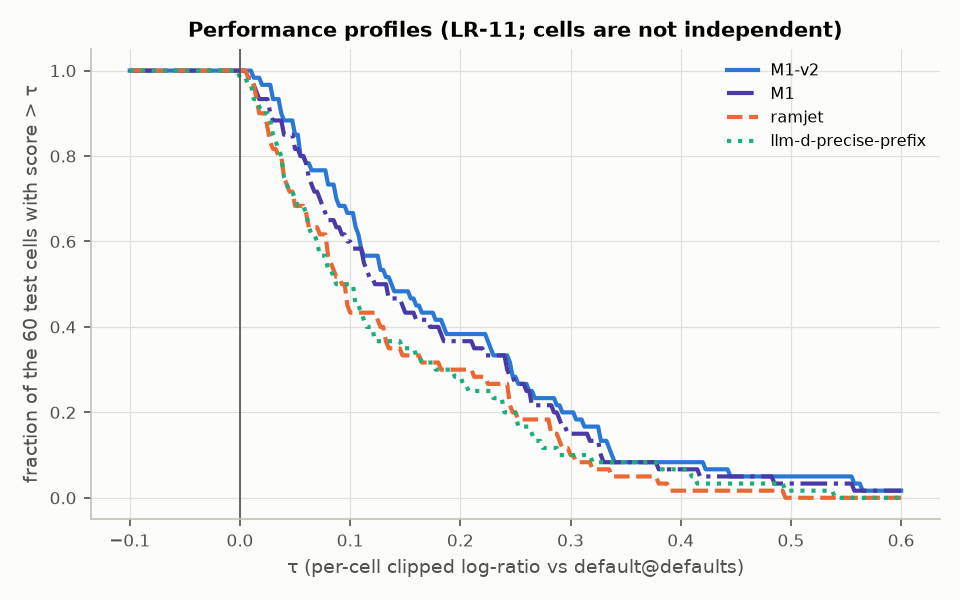
\includegraphics[width=0.6\linewidth]{performance_profiles}
  \caption{Performance profiles over the 60 test cells (copied from the final report): the fraction
    of cells on which a policy's clipped log-ratio against $\piref$ exceeds $\tau$. Cells are not
    independent, so the profiles are descriptive.}
  \label{fig:profiles}
\end{figure}

% SPDX-FileCopyrightText: Copyright (c) 2026 NVIDIA CORPORATION & AFFILIATES. All rights reserved.
% SPDX-License-Identifier: Apache-2.0
%
% ROLE: the pilot that gated phase 2, kept for the record. Every number is preliminary (pilot,
%   validation split or train subset) and was superseded by the phase-2 tuning and the test pass.
%   Reader-facing text calls phase 2 "the main tuning" and the phase-2 midpoint "mid-tuning"
%   (restructure plan, section 2.17; app:provenance maps the names).
% EVIDENCE: CR/facts/pilot.json, CR/facts/gate.json.
% UNITS (read before editing): "segment mean" and the MDE are in units of the paired goodput
%   ratio minus one, G(pi)/G(pi') - 1, without eps and unclipped (learned_routing/noise.py
%   differs_beyond_noise; CR/runs/gate/scripts/recompute_gate.py verdict). "Mean Delta" columns
%   are clipped log-ratios with eps (eq:clr). The two agree to first order at these sizes.

\section{The pilot (preliminary)}
\label{sec:pilot}

The pilot asked whether tuning moves any policy away from the default router by more than
replicate noise, and how large the learned model's margin over the best heuristics might be,
before the study committed to the main tuning. Its numbers come from the validation split and from
a smaller tuning setup than the main tuning, so they are \prelim{} and were superseded by the results
of the main tuning and the test pass (\cref{sec:results}). They are kept because they shaped the main
tuning: the budget, the step-size cap, the multi-start initialization, the extended feature set and
the concentration audit all trace back to them.
% src: CR/facts/pilot.json decisions, train_subset, runs, selected; CR/facts/STATE.md pilot(phase3)

The setup was smaller than the main tuning's in four ways.
\begin{itemize}
  \item M0 (the default cost, tuned) and M1 (\lc{} on feature set \code{v1}) were tuned on 12 of
    the 34 train cells, chosen to cover every family, both train worker counts and every load
    mode, with 480 evaluations (30 generations of 16) per run.
  \item Each model was tuned twice with different CMA-ES seeds from the \emph{same} start
    (M1 from $\theta = -\basis{0}$, M0 from the shipped defaults). Below they are called seed 1
    and seed 2; they are not the main tuning's restarts 1 to 3, which differ in their start.
  \item The configuration of each model was selected on validation replicates $\krep = 0, 1, 2$
    over both seeds and their checkpoints: seed 1 at generation 25 for M0, seed 2 at generation
    30 for M1.
  \item The heuristics were not tuned. A screen of all nine catalog heuristics at shipped
    defaults on the 12 train cells ($\krep = 0, 1$) ranked \policy{llm-d-precise-prefix}
    ($+0.169$), \policy{ramjet} ($+0.166$) and \policy{lmetric} ($+0.165$) first by mean clipped
    log-ratio; the last two are tied, so all three went to validation. \policy{dualmap}
    ($-0.150$) and \policy{chwbl} ($-0.214$) lost to the default on that subset.
\end{itemize}
% src: CR/facts/pilot.json heuristic_screen_train_subset.mean_clipped_log_ratio, ranking, sanity_note
All policies were then scored on the 14 validation cells with 8 fresh replicates
($\krep = 3,\dots,10$) that no selection step had used, paired with $\piref$ on the same
replicate. The pilot ran \num{56552} fresh replays with 0 errors, and an independent judge,
working from the raw records without importing the harness, reproduced every comparison against
$\piref$ and against the heuristics in \cref{tab:pilot,tab:pilot-h2h} to four decimals.

``Beyond noise'' below is the study's two-clause rule (\cref{sec:noise-floor}): on some cell
the replicate-mean goodput ratio to the reference departs from 1 by more than three pooled
replicate standard deviations, and over at least three independent segments the mean of the
per-segment mean of (ratio $-\,1$) exceeds twice its standard error in absolute value. The rule
is two-sided, so a policy worse than the reference also passes it.
% src: CR/CONTRACT.md A1 ("Differs beyond noise"); WT/benchmarks/learned_routing/learned_routing/noise.py
%      differs_beyond_noise (k_sd 3, k_se 2, min_segments 3)
% src: CR/facts/gate.json criteria.1_error_rate, selection_hygiene.val_k3_10_unused_by_selection,
%      context_not_gate.agreement_with_pilot ("every vs-default and vs-heuristic number ... reproduces to 4 decimals")

\begin{table}[tbp]
  \centering\footnotesize
  \setlength{\tabcolsep}{4pt}
  \caption{Pilot, validation split, every policy against $\piref$ (\prelim). Mean $\clr$: mean
    over cells of the replicate-mean clipped log-ratio, overall and per family (Mooncake 5 cells,
    sessions 5, AgentX 4). Ratio: mean over cells of the replicate-mean goodput ratio
    $\Gw(\pol)/\Gw(\piref)$. Better: cells whose mean ratio exceeds 1. Seg.\ mean (SE):
    mean over the 6 validation segments of the per-segment mean of (ratio $-\,1$), with its
    standard error. Over cap: cells on which, in at least one replicate, one worker received more
    than $\min(2/\Nw,\ 1/\Nw + 0.25)$ of the requests.}
  \label{tab:pilot}
  % src: CR/facts/pilot.json validation_k3_10_vs_default.policies.<name>: mean_clipped_log_ratio,
  %      by_family_mean_clipped_log_ratio.{mooncake,synthetic_sessions,agentx}, mean_ratio,
  %      cells_better, mean_segment_delta, segment_se, worker_share_cap_exceeded_cells.
  %      Rounded to 3 places. Cross-check: CR/facts/gate.json criteria.3_differs_beyond_noise.vs_default.
  \begin{tabular}{@{}lrrrrrcrc@{}}
    \toprule
    & \multicolumn{4}{c}{Mean $\clr$} & & & & \\
    \cmidrule(lr){2-5}
    Policy & all & Mooncake & sessions & AgentX & Ratio & Better & Seg.\ mean (SE) & Over cap \\
    \midrule
    M1, seed 2 (selected)          & 0.165 & 0.221 & 0.205 & 0.045 & 1.191 & 13/14 & 0.147 (0.044) & 5 \\
    M1, seed 1                     & 0.162 & 0.220 & 0.200 & 0.043 & 1.187 & 13/14 & 0.142 (0.044) & 4 \\
    \policy{llm-d-precise-prefix}  & 0.135 & 0.124 & 0.203 & 0.064 & 1.153 & 14/14 & 0.135 (0.034) & 1 \\
    \policy{ramjet}                & 0.135 & 0.154 & 0.194 & 0.038 & 1.152 & 14/14 & 0.122 (0.038) & 0 \\
    \policy{lmetric}               & 0.133 & 0.116 & 0.208 & 0.060 & 1.150 & 14/14 & 0.132 (0.036) & 0 \\
    M0, seed 2                     & 0.129 & 0.129 & 0.194 & 0.047 & 1.145 & 14/14 & 0.124 (0.035) & 0 \\
    M0, seed 1 (selected)          & 0.128 & 0.128 & 0.198 & 0.041 & 1.144 & 14/14 & 0.121 (0.037) & 0 \\
    round-robin                    & $-0.577$ & $-0.273$ & $-0.892$ & $-0.562$ & 0.571 & 0/14 & $-0.473$ (0.066) & 0 \\
    \bottomrule
  \end{tabular}
\end{table}

\paragraph{Everything beat the default router; round-robin collapsed.}
Every tuned and heuristic policy in \cref{tab:pilot} differed from $\piref$ beyond noise, in the
positive direction, overall and separately in each load mode; round-robin differed in the negative
direction. The three cache-aware heuristics at shipped defaults already reached a mean per-cell
goodput ratio over $\piref$ of 1.150--1.153, and M1 reached 1.191. M0 was the weakest of the tuned
and heuristic policies: tuning the default cost's five knobs on 12 cells gained less than
switching to an untuned cache-aware heuristic. The bar M1 had to clear in the main tuning was
therefore set by those heuristics, after they got the same tuning budget, not by the default.
% src: CR/facts/gate.json criteria.3_differs_beyond_noise.per_mode_pass, policies_passing_per_mode;
%      CR/facts/pilot.json gate.condition_3_differs_beyond_noise.note

\paragraph{M1 against the strongest heuristic: not beyond noise.}
\Cref{tab:pilot-h2h} pairs the selected M1 and M0 directly with each heuristic. Against
\policy{llm-d-precise-prefix}, the validation-best heuristic, M1's mean clipped log-ratio was
$+0.030$ (mean ratio 1.032, 10 of 14 cells better). The pre-registered minimum detectable effect
(MDE) is $\max(1\%,\ 2\,\mathrm{SE})$, where SE is the standard error of the paired segment mean
on validation, in units of (ratio $-\,1$). At the pilot that SE was 0.019, so the MDE is 0.038.
M1's segment mean was only $+0.009$: the Mooncake window that carried the gain is 5 of the 14
cells but 1 of the 6 segments. Under the study's noise rule M1 did not differ from this
heuristic, overall or in any single load mode. The same held against \policy{ramjet} and
\policy{lmetric}, with one exception: M1's lead over \policy{ramjet} in closed loop ($+0.038$, SE
0.013, over 3 segments) passed the rule.
% src: CR/facts/pilot.json validation_vs_best_heuristic.llm-d-precise-prefix.M1_tuned; mde.learned_vs_val_best_default_arm_heuristic
%      (segment_se 0.019075, mde 0.038150); CR/facts/gate.json context_not_gate.learned_vs_best_default_arm_heuristic
%      ["m1-s2@sel-g30 vs ramjet@defaults"].by_mode.closed_concurrency (0.0380, SE 0.0127, differs true)

\begin{table}[tbp]
  \centering\footnotesize
  \setlength{\tabcolsep}{4pt}
  \caption{Pilot, validation split, head to head (\prelim): the selected M1 and M0 against each
    untuned heuristic, paired on the same replicates $\krep = 3,\dots,10$. Columns as in
    \cref{tab:pilot}; positive values favor the tuned model. Noise: whether the pair differs beyond
    noise under the rule defined above. MDE $= 0.038$ in the units of the segment mean.}
  \label{tab:pilot-h2h}
  % src: CR/facts/pilot.json validation_vs_best_heuristic.<heuristic>.{M1_tuned,M0_tuned}: mean_clipped_log_ratio,
  %      by_family_mean_clipped_log_ratio, mean_ratio, cells_better, mean_segment_delta, segment_se,
  %      differs_beyond_noise, differs_by_mode. M1 = m1-s2@sel-g30, M0 = m0-s1@sel-g25.
  \begin{tabular}{@{}lrrrrrcrl@{}}
    \toprule
    & \multicolumn{4}{c}{Mean $\clr$} & & & & \\
    \cmidrule(lr){2-5}
    Against & all & Mooncake & sessions & AgentX & Ratio & Better & Seg.\ mean (SE) & Noise \\
    \midrule
    \multicolumn{9}{@{}l}{\emph{M1 (seed 2, selected)}} \\
    \policy{llm-d-precise-prefix} & 0.030 & 0.097 & 0.002 & $-0.019$ & 1.032 & 10/14 & 0.009 (0.019) & no \\
    \policy{ramjet}               & 0.030 & 0.067 & 0.011 & 0.007    & 1.031 & 12/14 & 0.021 (0.011) & closed$^{a}$ \\
    \policy{lmetric}              & 0.032 & 0.105 & $-0.003$ & $-0.015$ & 1.034 & 6/14 & 0.012 (0.020) & no \\
    \midrule
    \multicolumn{9}{@{}l}{\emph{M0 (seed 1, selected)}} \\
    \policy{llm-d-precise-prefix} & $-0.007$ & 0.004 & $-0.005$ & $-0.023$ & 0.993 & 3/14 & $-0.012$ (0.006) & no \\
    \policy{ramjet}               & $-0.007$ & $-0.026$ & 0.004 & 0.003 & 0.993 & 7/14 & $-0.001$ (0.005) & no \\
    \policy{lmetric}              & $-0.005$ & 0.012 & $-0.010$ & $-0.019$ & 0.995 & 4/14 & $-0.010$ (0.005) & lanes$^{a}$ \\
    \bottomrule
    \multicolumn{9}{@{}l}{$^{a}$ Not beyond noise overall; beyond noise in this load mode only.}
  \end{tabular}
\end{table}

\paragraph{Where the margin came from.}
M1's lead over \policy{llm-d-precise-prefix} came from one of the six validation segments. Per
segment, the mean of (ratio $-\,1$) was $+0.102$ on the Mooncake window w1 (5 cells), $+0.003$ and
$+0.001$ on the session seeds s4 and s5, and $-0.014$, $-0.025$ and $-0.012$ on the three AgentX
play subsets V1--V3. On validation, then, M1 gained where requests share a few hot prefixes across
users, and lost slightly, but on every segment, on long agent contexts. That AgentX deficit shaped
the main tuning: M1's second and third restarts started from a behavior clone of
\policy{llm-d-precise-prefix} and from a cache-heavy point (\cref{sec:restarts}), and the 23-feature
set \code{v2} became a mandatory arm, the one that won.
% src: CR/facts/gate.json context_not_gate.m1_vs_llm_d_precise_prefix_segment_deltas;
%      audit_flags_for_stage4 ("whole lead from mooncake:w1"); CR/CONTRACT.md A11.1, A17.1

\paragraph{The lead came with concentration.}
Over all validation records, the selected pilot M1 exceeded the share cap on 5 Mooncake cells (27
of 112 cell-replicate records), with a largest share of 0.646 in one record;
\policy{llm-d-precise-prefix} exceeded it on one cell. This flag became the mid-tuning
gaming audit (\cref{sec:gaming}).
% src: CR/facts/gate.json context_not_gate.guards_worker_share["m1-s2@sel-g30"] (5 cells, 27 records,
%      max 0.6465), guards_worker_share (llm-d-precise-prefix: 1 cell), audit_flags_for_stage4

\begin{table}[tbp]
  \centering\footnotesize
  \caption{What the pilot M1 learned (\prelim). $s_f = \mathrm{sd}(x_0)/\mathrm{sd}(x_f)$, with
    within-set standard deviations measured on candidate tables reconstructed from $\piref$'s
    train replays; $\theta_f / s_f$ is the utility change per one within-set standard deviation of
    feature $f$, in units of the anchor's ($\theta_0 = -1$). The search bound was
    $|\theta_f| \le 4 s_f$.}
  \label{tab:pilot-theta}
  % src: CR/facts/pilot.json selected.M1_tuned.values (seed 2); runs.m1-s1.selected_by_val.values (seed 1);
  %      feature_scaling.pooled_within_set_sd. theta_f / s_f = theta_f * sd(x_f) / sd(x_0), computed
  %      2026-10-03 from those fields; s_f matches pilot.json decisions.
  \begin{tabular}{@{}rlrrrr@{}}
    \toprule
    $f$ & Feature & $s_f$ & $\theta_f$, seed 2 & $\theta_f/s_f$, seed 2 & $\theta_f/s_f$, seed 1 \\
    \midrule
    0 & \code{default\_logit\_scaled}     & 1     & $-1$ (pinned) & $-1$     & $-1$ \\
    1 & \code{overlap\_frac}              & 25.6  & 13.60   & 0.532    & 0.383 \\
    2 & \code{new\_prefill\_tokens\_k}    & 17.7  & $-8.71$ & $-0.493$ & $-0.143$ \\
    3 & \code{active\_prefill\_tokens\_k} & 5.33  & $-0.546$ & $-0.102$ & $-0.158$ \\
    4 & \code{kv\_load\_frac}             & 80.8  & $-0.434$ & $-0.005$ & 0.015 \\
    5 & \code{active\_requests\_s}        & 110   & $-49.2$ & $-0.449$ & $-0.407$ \\
    6 & \code{session\_affinity}          & 21.2  & 0.995   & 0.047    & 0.018 \\
    7 & \code{isl\_x\_prefill\_load}      & 3.22  & 0.041   & 0.013    & 0.021 \\
    \bottomrule
  \end{tabular}
\end{table}

\paragraph{What the pilot M1 learned.}
Relative to the default cost they start from, both pilot M1 seeds moved in three directions
(\cref{tab:pilot-theta}): more weight on the overlap fraction, a penalty on new prefill tokens
(strongly in seed 2 only), and a penalty on the number of active requests, a quantity the default
cost ignores at its shipped weight $\breq = 0$. Both tuned M0 configurations moved the same way
within their own family: more overlap credit ($\bov = 1.62$ and 1.65, shipped 1), a larger
prefill-load scale ($\bpf = 24.8$ and 16.9, shipped 1) and a nonzero active-request weight
($\breq = 854$ and \num{1152}, shipped 0), so that each active request costs as much as 34 or 68
prefill blocks. Two model classes tuned independently thus both added a request-count load term,
the direction the main tuning's M1-v2 took further with its prefill-by-requests interaction
(\cref{sec:res-coefficients}).
% src: CR/facts/pilot.json selected.M0_tuned.values (m0-s1: credit 1.6176, decay 1.5253, prefill_load_scale 24.823,
%      decode_active_request_weight 853.59, temperature 0.00197); runs.m0-s2.selected_by_val.values
%      (1.6536, 0.5756, 16.877, 1151.5, 0.0238). 853.59/24.823 = 34.4; 1151.5/16.877 = 68.2 (arithmetic).

\paragraph{How the search behaved.}
M1's validation score (the CMA-ES mean, on $\krep = 0,1,2$) reached 0.163--0.165 within 160--240
evaluations and then stayed within 0.005 of each run's maximum; the two seeds ended 0.0004 apart.
M0 plateaued within 80--160 evaluations on train, but in one seed the CMA-ES step size then grew
from 0.18 to 10.8 internal units and the generation mean fell to $-0.23$, a drift along
near-flat directions of the default cost's knobs. The main tuning therefore capped the per-coordinate
step size at 0.3 internal units and set the budget at 400 evaluations per run, the latest
validation plateau among the four pilot runs (\cref{sec:space,sec:noise}). On 16 candidates, the
objective on the 12-cell subset ranked candidates like the objective on all 34 train cells
(Spearman 0.947); the main tuning nevertheless tuned on all 34.
% src: CR/facts/pilot.json measurements.cma_progress_curves.summary; projection.inputs.plateau.runs.*.val_by_generation;
%      measurements.subset_vs_full_objective (spearman 0.947, n 16); recommendations_for_phase2;
%      CR/facts/gate.json full_plan.budget, objective_cells_repeats.cells ("all 34 train cells every evaluation")

% SPDX-FileCopyrightText: Copyright (c) 2026 NVIDIA CORPORATION & AFFILIATES. All rights reserved.
% SPDX-License-Identifier: Apache-2.0
%
% ROLE: enough identifiers for a teammate to rebuild any number in the paper: branch and commits,
%   versions, frozen-artifact hashes, the REPRODUCE.md procedure in summary, determinism and
%   cross-host parity evidence, entry points and where each stage's facts live. The step-by-step
%   procedure stays in WT/notes/learned-routing/REPRODUCE.md; do not duplicate its commands here.
% EVIDENCE: WT/notes/learned-routing/{README.md,REPRODUCE.md}; CR/facts/{setup,build_rust,integration,
%   test_freeze,remote,lag_patch,pilot,gate}.json; CR/facts/STATE.md; CR/facts/UPSTREAM_FOLLOWUPS.md;
%   CR/facts/DEVIATIONS.md; git log of WT (read 2026-10-03).
% STATUS: final for this draft. Internal commit hashes are deliberately not printed: the public copy
%   of the branch has different commits (public-content rule, A18). Name branches and files instead.
% PATHS: CR = campaign root (REPRODUCE.md calls it LR_ROOT); WT = the campaign worktree. Printed
%   paths are relative to those; do not print absolute home-directory paths.

\section{Reproducibility}
\label{app:repro}

The campaign's durable record is the directory \file{notes/learned-routing/} on the Dynamo
branch \code{rupei/learned-routing}, whose sanitized copy \code{rupei/learned-routing-public} is
public. \file{README.md} describes the
campaign and its state, \file{REPRODUCE.md} rebuilds it step by step on a clean Linux x86\_64
machine, and \file{campaign/} mirrors every small file the steps need: facts, cells, audits, run
summaries, calibration scripts and the AgentX base manifests. Bulky artifacts (traces, workload
replicates, the replay cache) stay in the campaign root and are regenerated from pinned public
sources. Off the original host, git and the public sources are enough for the steps
\file{REPRODUCE.md} covers. This appendix lists the
identifiers; the procedure is in \file{REPRODUCE.md}.
% src: WT/notes/learned-routing/README.md (intro, "Directory map", "Artifacts not in git"); REPRODUCE.md intro

\subsection{Branches}

% src: WT/notes/learned-routing/README.md; CR/CONTRACT.md "Paths", A5, A11.5, A16; CR/facts/lag_patch.json
%      worktree; CR/facts/ais_features.json worktree, build
The campaign's code and record live on three branches of the Dynamo repository.
\begin{itemize}
  \item \code{rupei/learned-routing}: the policies (\lc{} and \policy{sticky-session} in the builtin
    catalog, and the \code{seed} parameter on \defaultcf{}), the harness (\code{lr-eval},
    \code{lr-train}, \code{lr-report} and the remote CPU lane), the live lane, and the campaign notes
    under \file{notes/learned-routing/}, including this paper. It starts from the head of the
    router-policy pull-request stack (\#15450 and \#15453), which already runs catalog policies in
    offline replay and passes the device-tier overlap to them.
  \item \code{rupei/learned-routing-lag}: the router-state lag knob for offline replay, built
    separately so that the tuning build and its result cache stay untouched.
  \item \code{rupei/learned-routing-ais}: feature set \code{v3} and the research input for a
    request's modeled prefill time, also on its own build, for the \ais{} league.
\end{itemize}
Every stage's facts file records the worktree head it ran at. Only the first branch is published,
as the sanitized copy \code{rupei/learned-routing-public}, in which internal commits appear as
position labels; the lag and \ais{} branches are not, so the lag part of the robustness pass
and the \ais{} league can be checked against the mirrored facts but not yet rebuilt from public
sources.
% src: CR/CONTRACT.md A20 "Publication" (only the sanitized copy of the campaign branch is pushed);
%      CR/facts/robustness.json execution (lag records on the lag build, timing records on the tuning build)
\file{REPRODUCE.md} rebuilds the campaign to its calibrated, frozen cells; the later stages are
reproduced from the mirrored facts and the analysis scripts named in the final report's reproduction
section. \pending{a REPRODUCE.md revision that walks through the pilot, phase 2, the test pass and
the robustness pass}

\subsection{Environment}

% src: CR/facts/setup.json versions; CR/facts/build_rust.json correction_fix_r0.bindings;
%      CR/facts/test_freeze.json bindings_build_id, harness_version; CR/facts/lag_patch.json build;
%      REPRODUCE.md section 2 (host image), CR/facts/calibration.json compute (24 cores)
\begin{center}\footnotesize
\begin{tabularx}{\linewidth}{@{}lY@{}}
  \toprule
  Python, Rust & CPython 3.12.3; rustc 1.96.1 (pinned by \file{rust-toolchain.toml}); maturin 1.15.0 \\
  Simulator & \code{aisimulate} 0.13.0.dev202609300000000061 (wheel) and the matching
    \code{aisimulate-core} crate \\
  Dynamo & \code{ai-dynamo} and \code{ai-dynamo-runtime} 1.6.0, editable from the worktree \\
  Bindings & built with feature \code{ais-forward-pass} (required for \ais{} engine timing);
    \code{\_core.abi3.so} SHA-256 \code{1d67c131\ldots}, build ID \code{6955b0ee\ldots} \\
  Lag-check bindings & separate build, \code{.so} \code{90464b9b\ldots}, build ID \code{a6c6b04e\ldots} \\
  Harness & package \code{learned\_routing}, harness version \code{lrh-4} \\
  Python packages & \code{cma} 4.5.0, \code{numpy} 2.5.3, \code{scipy} 1.18.1, \code{pandas} 3.0.6,
    \code{matplotlib} 3.11.2 \\
  Host & Ubuntu 24.04, glibc 2.39, 24 cores; local replays share a pool of 20 slots \\
  \bottomrule
\end{tabularx}
\end{center}

The build ID is a hash of the bindings' shared object together with the simulator version, and
it is part of every result-cache key. A rebuild almost always yields a new ID, because the shared
object embeds build-tree paths, so cached results from another build are never reused by accident.
% src: REPRODUCE.md section 3 ("Build IDs"); UPSTREAM_FOLLOWUPS #7 (RPATH); learned_routing/cache.py bindings_build_id

\subsection{The rebuild procedure in brief}

\Cref{tab:reproduce} condenses \file{REPRODUCE.md}. ``Verified'' there means the step was re-run
while the notes were written, on the campaign host or in a fresh private root.

\begin{table}[tbp]
  \centering\footnotesize
  \caption{Sections of \file{REPRODUCE.md} and what each establishes.}
  \label{tab:reproduce}
  % src: WT/notes/learned-routing/REPRODUCE.md sections 1-17 and its "What reproduces exactly" list
  \begin{tabularx}{\linewidth}{@{}rlY@{}}
    \toprule
    \S & Step & What it establishes, and how it was checked \\
    \midrule
    1 & Branch and SHAs & worktree at the snapshot commit; base is an ancestor \\
    2--3 & Environment, bindings & pinned versions; the KV-capacity estimate (\num{18863} blocks) and a
      one-request replay whose TTFT equals the \ais{} value prove \ais{} timing is in effect \\
    4 & Harness and tests & Rust policy tests (127 pass, 2 pre-existing ignored) and harness tests \\
    5 & Campaign root & \file{config/engine.json} copied from git and checked by SHA-256; every
      \code{DYN\_ROUTER\_*} variable unset, since replay workers inherit them and they change policies
      without changing the cache key \\
    6 & Traces & source traces regenerated byte-identically (106 of 106 files, verified) \\
    7 & Cells & frozen cells \code{lr-cells-v5} installed from git, not regenerated \\
    8 & AgentX lowering & six base manifests from git; lowering checked field for field by an
      independent re-implementation for all 82 plays and 6 transforms \\
    9 & Derived traces & every trace the frozen cells reference regenerated byte-identically (34/34
      train, 14/14 validation, 60/60 test cells, verified); then a parity smoke against a mirrored
      reference (4 identical, 0 different) \\
    10 & Calibration & mirrored driver scripts; every load level follows from the mirrored load curves
      (171/171 levels and 108/108 cell loads, verified) \\
    11 & Frozen test set & SHA-256 of \file{cells/test.jsonl} and of every test trace \\
    12 & Replicates & the replicate protocols, policy seeds and the noise rule \\
    13 & Entry points & \code{lr-eval}, \code{lr-train}, \code{lr-report}; the remote bundle flow and
      the cluster CPU lane \\
    14 & Gate and headline & the pilot gate and the pre-registered headline test \\
    15 & Later stages & listed as not yet run when the notes were written (see above) \\
    16--17 & Costs, mirrored files & measured costs; the small files that used to live only in the
      campaign root \\
    \bottomrule
  \end{tabularx}
\end{table}

\subsection{Frozen inputs}

% src: CR/facts/test_freeze.json (engine_json_sha256, test_jsonl, traces, split_manifest_sha256,
%      traces_manifest_sha256, written 2026-10-03 01:53:07 PDT); WT/notes/learned-routing/README.md
%      ("Frozen test traces (39 files, 2,130,865,265 bytes)"); CR/facts/HEADLINE_TEST.json
\begin{itemize}
  \item Engine configuration \file{config/engine.json}, SHA-256 \code{7b5ff164\ldots}: the single source
    of truth for model, hardware, backend, parallelism, context length and engine arguments.
  \item Cells \code{lr-cells-v5}: test file \file{cells/test.jsonl}, SHA-256 \code{7b998b8e\ldots};
    split manifest, SHA-256 \code{0e84edf1\ldots}. The freeze record \file{facts/test_freeze.json}
    also hashes the content of every test cell and all 39 test traces (\num{2130865265} bytes).
  \item Source traces, pinned by SHA-256 in \file{traces/MANIFEST.json} (\code{b2616d0d\ldots}).
  \item The headline test, pre-registered in \file{facts/HEADLINE_TEST.json} before any training.
  \item Before the single test pass the test stage verified all 149 freeze hashes, and
    \file{facts/finalists.json} was frozen (SHA-256 \code{e0bae29d\ldots}) before the first test record.
\end{itemize}
% src: CR/facts/test_results.json execution.evaluated_once (149/149; finalists.json sha256 e0bae29d)

\subsection{Determinism}
\label{app:determinism}

Replay is deterministic: the same policy on the same cell and replicate reproduces every
per-request row. The campaign relies on this in four places.
\begin{itemize}
  \item \textbf{Seeds.} The shipped default router broke ties with an unseeded random number
    generator, so identical runs of one Mooncake cell gave different goodput (2.8934 against 2.8290
    for the catalog policy). The branch adds a \code{seed} parameter. The harness passes seed
    $\krep + 1$ to the seeded policy types (\defaultcf{}, \lc{}, \policy{sticky-session}); every
    other type takes no seed.
    % src: CR/facts/UPSTREAM_FOLLOWUPS.md #1; REPRODUCE.md section 12 "Policy seeds"
  \item \textbf{Replicates.} Variation comes from workload replicates shared by every policy:
    replicate $\krep$ permutes arrivals logged at the same instant (protocol \code{crn-order-v1}),
    re-draws each session's first arrival inside its logging slot (\code{crn-spread-v1}, for traces
    logged on a grid), or permutes recycled AgentX copies.
    % src: REPRODUCE.md section 12 (protocol table)
  \item \textbf{Parity with the default.} \lc{} at $\theta = -\basis{0}$, with the tie-break that
    replays the default picker's random stream, chose the same worker as the seeded \defaultcf{} on
    every request of 88 of 88 (cell, replicate) pairs, and again on 22 of 22 after the bindings were
    rebuilt. With the tie-break used in training (\code{one\_draw}) individual ties resolve
    differently, but goodput did not differ beyond noise.
    % src: CR/facts/integration.json parity (exact_reservoir 88/88; one_draw_noise_rule differs false);
    %      CR/facts/STATE.md fix(build r0) ("theta0-reservoir == default 22/22 post-rebuild")
  \item \textbf{Re-runs and resumes.} An independent calibration audit re-ran replicates 0 and 1 of
    11 cells for $\piref$ and round-robin and matched the cache on 44 of 44 records, every field and
    every per-request byte; new replicates run twice were identical on 44 of 44. A harness audit
    killed \code{lr-train} three times by process ID and the resumed runs were bit-identical,
    including their continuation.
    % src: CR/facts/STATE.md audit(calibration/independent-rerun r1) ("k0,1 == calibration cache 44/44 ...
    %      new k10,11 run twice 44/44 identical"); audit(build/harness-robustness-splits r1)
    %      ("lr-train 3x kill -9 exact PIDs resume bit-identical incl. continuation")
\end{itemize}
Results are cached under a SHA-256 of the canonical policy, the cell identifier and content, the
replicate and its protocol, the harness version and the bindings build ID. One residual
nondeterminism is harmless: replay orders its per-request output by random request identifiers, so
summary means can differ in the last bits ($\sim 10^{-15}$ relative); the harness recomputes every
metric from a sorted copy of the rows.
% src: CR/facts/DEVIATIONS.md build B3 "cache key"; CR/facts/UPSTREAM_FOLLOWUPS.md #2

\subsection{Cross-host parity}
\label{app:parity}

Replay calls the host's math library, so bit-exact results require the same OS and C library
image. Most tuning ran on a pool of shared CPU nodes, one run per node, from a self-contained bundle holding the exact local shared object, the harness, the traces
and the cells. Before any node image was used, a parity smoke compared its records with the
workstation's.
\begin{itemize}
  \item \textbf{Lane validation.} Ten comparisons on AMD EPYC 7702P and EPYC 9654P nodes (Ubuntu
    24.04.5, glibc 2.39, CPython 3.12.3) were all identical: \num{6312} remote records with no field
    differences, and \num{48901384} per-request rows byte-identical. They covered seven cells
    (Mooncake open and closed loop, sessions, lowered AgentX, including one AgentX cell at
    $\Nw = 16$), six replicas of the calibration reference batch, and two short tuning runs.
  \item \textbf{Tuning numerics.} With default settings, \code{numpy} and OpenBLAS dispatch AVX-512
    kernels on the EPYC 9654P, and the CMA-ES state differed from the workstation's in the last bits
    from the first generation. The node scripts pin the dispatch (\code{OPENBLAS\_CORETYPE=Haswell},
    \code{OPENBLAS\_NUM\_THREADS=1}, \code{NPY\_DISABLE\_CPU\_FEATURES}); with the pins, a 60-generation
    check matched the workstation on every generation on both CPU types, and the remote tuning
    smoke runs wrote byte-identical histories, best points and policy files.
  \item \textbf{Test pass.} Tasks that ran twice, once in a first wave and again after a timeout
    fix, were bit-identical on different nodes in every field and per-request byte.
  \item \textbf{Pilot and phase 2.} The 384 records of the pilot's 16 first-generation candidates on
    the 12 subset cells were identical locally and on the cluster. A node image added during
    phase 2 passed its smoke (28 of 28 records, \num{186548} rows) before it ran any tuning.
  \item \textbf{Lag build.} The separate lag-check build was validated on five node images before
    the robustness pass (the first: 192 of 192 records, \num{1214112} rows).
\end{itemize}
% src: CR/facts/remote.json summary, environment, parity.totals ("10 comparisons, all IDENTICAL: 6,312 remote
%      records ... 48,901,384 per-request rows"), parity.core_6_train_cells.cells, parity.step4_replicas,
%      parity.lr_train.numerics_check (EPYC 9654P default 0/60; pinned 60/60), a later node image's
%      parity entry (28/28, 186,548), parity.lag_build_a6c6b04e (192/192, 1,214,112); CR/facts/robustness.json
%      execution.lag_build (5 node images); CR/facts/test_results.json execution.duplicate_parity; CR/facts/pilot.json
%      measurements.cross_host_bitwise (384/384); CR/CONTRACT.md A9 addendum, A10
%      UPSTREAM_FOLLOWUPS #11 (numerics)

\subsection{Entry points and stage facts}

Three command-line tools carry every number: \code{lr-eval} evaluates policies on cells with
replicates, through the slot pool and the cache; \code{lr-train} runs \cref{alg:train}; and
\code{lr-report} builds paired tables with segment-bootstrap intervals and refuses to pool records
from different builds or cell contents. Every long job is resumable and takes
\code{--max-wall-seconds}. A policy is one JSON or YAML object, and the tuned result
\file{best_policy.yaml} is itself a valid policy for \code{lr-eval}.
% src: REPRODUCE.md section 13

Each stage writes one facts file under \file{facts/} and one line in the append-only
\file{facts/STATE.md}: setup, the three build stages and their fixes, AgentX lowering, noise,
calibration and its fix, the test freeze, the pre-registered headline test, the cluster lane, the
pilot, the gate, phase-2 preparation, the lag patch, the \ais{} features
(\file{facts/ais\_features.json}), the tier-A and tier-B/C tuning (\file{facts/tierA.json},
\file{facts/tierBC.json}) and the phase-2 midpoint fix (\file{facts/phase2\_mid\_fix.json}), the
SLO-transfer constants (\file{facts/sla\_transfer\_spec.json}), the frozen finalists
(\file{facts/finalists.json}), the single test pass (\file{facts/test\_results.json} with its
\code{report\_must\_state} wording), the robustness pass (\file{facts/robustness.json}), the
secondary metrics (\file{facts/secondary\_metrics\_test.json}), the in-class heuristic diagnostic
(\file{facts/fairness\_in\_class\_heuristic.json}), the live lane (\file{facts/live.json},
\file{facts/live\_smoke.json}, \file{facts/live\_loadgen\_parity.json}), the live finalist runs
(the registration \file{facts/live\_plan.json} and the analysis \file{facts/live\_results.json}) and
this paper's derived numbers (\file{facts/paper\_draft.json}, \file{facts/paper\_final.json}). Every
audit report is under \file{audits/}, and the final report is \file{report/REPORT.md}; its live
section is also \file{report/LIVE.md}. The live analysis is reproducible from the raw load-generator
exports: \file{runs/live/finalists/scripts/live\_results.py} \code{verify} re-scores every live run
and requires identical scores, and \code{build} re-runs the registered analysis and writes the live
facts, \file{report/LIVE.md} and the report's table fragment, from which \code{make tables} copies the
live tables of \cref{sec:live}.
% src: CR/facts/ directory listing (2026-10-05); CR/report/REPORT.md section 14 "Live validation (§15)";
%      CR/facts/live_results.json reproduction

\paragraph{Footprint.}
On 2026-10-03 the campaign root held 95\,GB of traces and 247\,GB of run outputs, mostly workload
replicates (183\,GB) and the result cache (37\,GB); all of it regenerates from the steps above.
Compute per stage is in \cref{tab:cost}.
% src: REPRODUCE.md section 16 "Disk" (du at 02:14 PDT)

\subsection{Building this document}

The sources are in \file{notes/learned-routing/paper/}; \code{make} there runs \code{latexmk} with
\code{pdflatex} and BibTeX and writes \file{build/main.pdf}, and \code{make tables}, given the
campaign root, regenerates \file{generated/} from the final report's table fragments. The figures in
\file{fig/} are copies of the final report's. Every number in the text carries a source comment
(\code{\% src:}) naming the campaign file it comes from, and results that do not exist yet are
marked with a boxed \textsc{pending} tag.


\end{document}
